\documentclass[11pt,oneside]{book}

% ============================================================================
% PACKAGES
% ============================================================================

% Math packages
\usepackage{amsmath, amssymb, amsthm, mathtools}
\usepackage{bm}

% Graphics
\usepackage{graphicx}
\usepackage{tikz}
\usepackage{pgfplots}
\pgfplotsset{compat=1.18}

% Tables
\usepackage{booktabs}
\usepackage{multirow}
\usepackage{array}

% Colors
\usepackage{xcolor}
\definecolor{deepblue}{RGB}{0,51,102}
\definecolor{darkgreen}{RGB}{0,100,0}
\definecolor{darkred}{RGB}{139,0,0}

% Algorithms
\usepackage[ruled,vlined,linesnumbered]{algorithm2e}

% Code listings
\usepackage{listings}
\lstset{
    language=Python,
    basicstyle=\ttfamily\small,
    keywordstyle=\color{deepblue},
    commentstyle=\color{darkgreen},
    stringstyle=\color{darkred},
    showstringspaces=false,
    breaklines=true,
    frame=single,
    numbers=left,
    numberstyle=\tiny\color{gray}
}

% Hyperlinks
\usepackage{hyperref}
\hypersetup{
    colorlinks=true,
    linkcolor=deepblue,
    citecolor=darkgreen,
    urlcolor=deepblue,
    bookmarksdepth=3
}
\usepackage[capitalise,noabbrev]{cleveref}

% Page layout
\usepackage[margin=1in]{geometry}
\usepackage{fancyhdr}
\pagestyle{fancy}
\fancyhf{}
\fancyhead[RO,LE]{\thepage}
\fancyhead[LO]{\leftmark}
\fancyhead[RE]{\rightmark}

% Typography
\usepackage{microtype}
\usepackage{setspace}
\onehalfspacing

% Bibliography
\usepackage[style=alphabetic,sorting=nyt,maxbibnames=99]{biblatex}
\addbibresource{references.bib}

% Index
\usepackage{makeidx}
\makeindex

% Theorem environments
\theoremstyle{definition}
\newtheorem{definition}{Definition}[chapter]
\newtheorem{example}{Example}[chapter]
\newtheorem{exercise}{Exercise}[chapter]

\theoremstyle{plain}
\newtheorem{theorem}{Theorem}[chapter]
\newtheorem{lemma}[theorem]{Lemma}
\newtheorem{proposition}[theorem]{Proposition}
\newtheorem{corollary}[theorem]{Corollary}

\theoremstyle{remark}
\newtheorem{remark}{Remark}[chapter]
\newtheorem{note}{Note}[chapter]

% Custom commands for notation
\newcommand{\R}{\mathbb{R}}
\newcommand{\N}{\mathbb{N}}
\newcommand{\Z}{\mathbb{Z}}
\newcommand{\C}{\mathbb{C}}
\newcommand{\vx}{\mathbf{x}}
\newcommand{\vy}{\mathbf{y}}
\newcommand{\vz}{\mathbf{z}}
\newcommand{\vh}{\mathbf{h}}
\newcommand{\vw}{\mathbf{w}}
\newcommand{\vb}{\mathbf{b}}
\newcommand{\vq}{\mathbf{q}}
\newcommand{\vk}{\mathbf{k}}
\newcommand{\vv}{\mathbf{v}}
\newcommand{\va}{\mathbf{a}}
\newcommand{\vc}{\mathbf{c}}
\newcommand{\vf}{\mathbf{f}}
\newcommand{\vi}{\mathbf{i}}
\newcommand{\vo}{\mathbf{o}}
\newcommand{\vr}{\mathbf{r}}
\newcommand{\vt}{\mathbf{t}}
\newcommand{\vu}{\mathbf{u}}
\newcommand{\vp}{\mathbf{p}}
\newcommand{\vg}{\mathbf{g}}
\newcommand{\vn}{\mathbf{n}}
\newcommand{\vs}{\mathbf{s}}
\newcommand{\mA}{\mathbf{A}}
\newcommand{\mB}{\mathbf{B}}
\newcommand{\mC}{\mathbf{C}}
\newcommand{\mW}{\mathbf{W}}
\newcommand{\mX}{\mathbf{X}}
\newcommand{\mY}{\mathbf{Y}}
\newcommand{\mQ}{\mathbf{Q}}
\newcommand{\mK}{\mathbf{K}}
\newcommand{\mV}{\mathbf{V}}
\newcommand{\mH}{\mathbf{H}}
\newcommand{\mI}{\mathbf{I}}
\newcommand{\mU}{\mathbf{U}}
\newcommand{\mJ}{\mathbf{J}}
\newcommand{\mE}{\mathbf{E}}
\newcommand{\mM}{\mathbf{M}}
\newcommand{\mZ}{\mathbf{Z}}
\newcommand{\mT}{\mathbf{T}}
\newcommand{\mR}{\mathbf{R}}
\newcommand{\mF}{\mathbf{F}}
\newcommand{\mS}{\mathbf{S}}
\newcommand{\mO}{\mathbf{O}}
\newcommand{\mP}{\mathbf{P}}
\newcommand{\transpose}{^\top}
\newcommand{\norm}[1]{\left\|#1\right\|}
\newcommand{\abs}[1]{\left|#1\right|}
\newcommand{\dimof}[1]{\text{dim}(#1)}

% Custom boxes
\usepackage{framed}
\definecolor{keypoint-bg}{RGB}{227, 242, 253}
\definecolor{impl-bg}{RGB}{232, 245, 233}
\definecolor{caution-bg}{RGB}{255, 235, 238}

\newenvironment{keypoint}{%
  \def\FrameCommand{\fboxsep=8pt\colorbox{keypoint-bg}}%
  \MakeFramed{\advance\hsize-\width\FrameRestore}%
  \noindent\textbf{Key Point:}\par\vspace{4pt}%
}{\endMakeFramed}

\newenvironment{implementation}{%
  \def\FrameCommand{\fboxsep=8pt\colorbox{impl-bg}}%
  \MakeFramed{\advance\hsize-\width\FrameRestore}%
  \noindent\textbf{Implementation:}\par\vspace{4pt}%
}{\endMakeFramed}

\newenvironment{caution}{%
  \def\FrameCommand{\fboxsep=8pt\colorbox{caution-bg}}%
  \MakeFramed{\advance\hsize-\width\FrameRestore}%
  \noindent\textbf{Caution:}\par\vspace{4pt}%
}{\endMakeFramed}

% ============================================================================
% DOCUMENT INFORMATION
% ============================================================================

\title{
    {\Huge\bfseries Deep Learning and LLMs for Technical Leaders}\\[0.5cm]
    {\Large A Practical Guide to Understanding and Deploying Transformer Models}\\[0.5cm]
    {\large From Mathematical Foundations to Production Systems}
}
\author{[Author Name]}
\date{2026}

% ============================================================================
% DOCUMENT BODY
% ============================================================================

\begin{document}

% Front matter
\frontmatter
\maketitle

% Copyright page
\thispagestyle{empty}
\vspace*{\fill}
\begin{center}
\textcopyright{} 2026. All rights reserved.\\[1cm]
First Edition\\[0.5cm]
ISBN: [To be assigned]
\end{center}
\vspace*{\fill}
\clearpage

% Table of Contents
\tableofcontents
\clearpage

% List of Figures
\listoffigures
\clearpage

% List of Algorithms
\listofalgorithms
\clearpage

% Preface
\chapter*{Preface}
\addcontentsline{toc}{chapter}{Preface}

\section*{Why This Book?}

It's 3 PM on a Tuesday. Your VP of Engineering presents three proposals: (1) Fine-tune GPT-4 on your support tickets—\$180K investment; (2) Build a RAG system with embeddings—\$25K investment; (3) Prompt-engineer GPT-3.5—\$2K experiment. All three promise "85\% automation of tier-1 support." Which do you choose?

If you can't confidently evaluate these trade-offs, this book is for you. You're not alone—most technical leaders face AI decisions daily without the foundation to distinguish genuine engineering trade-offs from vendor hype.

Model architecture decisions—dimensions, layers, parameter counts—directly determine infrastructure requirements, operational costs, and system performance. Understanding the relationship between architectural choices and resource consumption is essential for evaluating technical proposals, planning infrastructure investments, and making informed build-versus-buy decisions. The computational characteristics of neural networks follow predictable patterns. A model's parameter count, layer structure, and dimensional choices create specific memory footprints and computational demands. These relationships aren't linear: doubling a model's dimensions typically quadruples memory requirements and increases computation eightfold. Recognizing these scaling behaviors enables accurate cost forecasting and realistic performance expectations.

This book provides the engineering foundation to evaluate AI systems, assess proposals, and make informed infrastructure and architectural decisions.

\section*{Who This Book Is For}

If you're a technical leader who needs to understand AI systems without becoming an ML researcher, this book is for you:

\begin{itemize}
    \item \textbf{CTOs and VPs of Engineering} making architecture and budget decisions
    \item \textbf{Technical Directors} evaluating team proposals and vendor claims
    \item \textbf{Principal Engineers} moving into leadership roles
    \item \textbf{Product Leaders} with technical backgrounds guiding AI strategy
    \item \textbf{Technical Architects} designing systems that incorporate AI
\end{itemize}

You don't need a machine learning background. You do need curiosity about how things work and willingness to think through engineering trade-offs.

\section*{What You Will (and Won't) Be Able To Do}

After reading this book, you will be able to evaluate whether a proposal to "train a 7B parameter model" is reasonable for your use case, question claims that "GPT-4 is required" when GPT-3.5 might suffice at one-tenth the cost, and estimate that doubling model dimensions increases compute 8×, not 2×. You will recognize when RAG will outperform fine-tuning at one-twentieth the cost and challenge proposals that ignore inference costs, which often exceed training costs by 100× annually.

You will NOT learn to write PyTorch training loops or implement attention mechanisms, fine-tune models yourself or debug CUDA errors, compete with ML engineers on implementation details, write research papers or contribute to academic ML, or perform detailed prompt engineering or low-level GPU programming.

These boundaries matter because your role is strategic—making informed decisions, asking the right questions, and allocating resources effectively. Implementation is your team's job; knowing when their answers make sense is yours. For implementation details, direct your team to PyTorch and TensorFlow documentation for coding, research papers for cutting-edge techniques, and framework-specific communities for troubleshooting. This book teaches you to evaluate, decide, and lead—not to implement.

\section*{Is This Book For You? A Quick Diagnostic}

Can you answer these questions confidently?

\begin{enumerate}
    \item Your team proposes a 12-layer, 768-dimensional transformer. Roughly how much memory is needed just to store the parameters? (Answer: ~440 MB for 110M parameters)
    \item A vendor claims their "optimized" model runs 3× faster. What should you ask? (Answer: Compute-bound or memory-bound? Batch size? Context length? Precision?)
    \item Fine-tuning costs \$5K. Expected inference volume is 10M requests/month. When does the investment pay back? (Answer: Depends on per-request cost reduction—need both numbers)
\end{enumerate}

If these questions feel abstract or you're unsure how to approach them, this book will give you the frameworks to answer them systematically.

\section*{How This Book Helps You Make Better Decisions}

\subsection*{The Leadership Challenge}

As a technical leader, you face AI proposals daily: "We should fine-tune GPT-4 on our data" (\$180K), "Let's train a custom 7B parameter model" (\$500K), "We need 32K context windows for our use case" (4× cost increase). How do you evaluate these? This book provides the frameworks.

\subsection*{Concept-to-Decision Map}

Every technical concept in this book maps directly to decisions you'll face:

\begin{table}[h]
\centering
\small
\begin{tabular}{p{4cm}p{4.5cm}p{2cm}}
\toprule
\textbf{When your team proposes...} & \textbf{You need to understand...} & \textbf{From chapter...} \\
\midrule
"Double model dimensions" & Cubic scaling (O(n³))—costs increase 8×, not 2× & 1.1.3 \\
"Train for 10 GPU-days" & Memory requirements (14× rule), optimizer overhead & 1.2.2, 2.4 \\
"Extend context to 16K tokens" & Quadratic attention scaling—costs 4× more & 3.3.1 \\
"Fine-tune vs. prompt engineering" & Cost crossover analysis, data requirements & 6.1-6.2 \\
"Self-host vs. use APIs" & Fixed vs. variable cost structures, volume thresholds & 7.3, 10.1.1 \\
"Use GPT-4 vs. GPT-3.5" & Quality-cost trade-offs, task complexity & 5.6, 10.2.2 \\
\bottomrule
\end{tabular}
\end{table}

\subsection*{Three-Layer Understanding Model}

\textbf{Layer 1: Mechanics (Part I—Chapters 1-3)}

What you'll learn: How systems work at a fundamental level. Why it matters: You can't spot unreasonable claims without understanding costs. Key output: "Is this proposal technically feasible and properly costed?"

\textbf{Layer 2: Choices (Parts II-III—Chapters 4-9)}

What you'll learn: Which approaches work for which problems. Why it matters: Most projects fail from wrong architectural choices, not implementation. Key output: "Is this the right approach for our constraints?"

\textbf{Layer 3: Decisions (Parts IV-V—Chapters 10-17)}

What you'll learn: When to build, buy, or walk away. Why it matters: Best implementation of wrong solution equals wasted money. Key output: "Should we do this at all?"

\subsection*{What Success Looks Like}

After reading this book, you'll be able to spot when "8 GPUs" doesn't match the proposed model size in proposal reviews, question whether fine-tuning is necessary or prompt engineering would suffice at one-twentieth the cost, and recognize when inference costs will dwarf training costs and demand the full analysis. In vendor conversations, you'll ask "At what batch size and percentile?" when they quote latency, demand clarification when "accuracy" is cited without baseline or metric, and calculate TCO over 3 years, not just sticker price. In strategic planning, you'll estimate that RAG system will cost \$500-1K/month versus \$50K one-time for fine-tuning, know that moving from GPT-3.5 to GPT-4 is 10-20× more expensive and when that's justified, and recognize when simpler rule-based systems would suffice.

\section*{Book Structure: Your Learning Path}

\begin{center}
\texttt{Part I (Foundations) → Part II (Architecture) → Part III (Production) → Part IV (Applications) → Part V (Synthesis)}\\
\vspace{0.3em}
\texttt{Ask: "How?" \hspace{1.5em} Ask: "Which?" \hspace{1.5em} Ask: "How much?" \hspace{1.5em} Ask: "Should we?" \hspace{1.5em} Ask: "What's next?"}
\end{center}

\textbf{Part I: Foundations (Chapters 1-3)}

Foundation for understanding how systems work at a fundamental level. Read first. You'll learn why costs scale non-linearly and what drives resource requirements.

\textbf{Part II: Architecture \& Infrastructure (Chapters 4-7)}

Framework for evaluating which technical approaches to choose. Essential for proposal evaluation. Covers training, deployment, optimization techniques, hardware.

\textbf{Part III: Production Layer (Chapters 8-9)}

Infrastructure reality—how much will this actually cost to build and run? Critical before commitment. Data pipelines, operational costs, lifecycle management.

\textbf{Part IV: Industry Applications (Chapters 10-15)}

Domain-specific patterns and should we build this decision frameworks. Use case driven. Jump to your domain or read sequentially for pattern recognition.

\textbf{Part V: Strategic Synthesis (Chapters 16-17)}

Strategic integration and future-proofing frameworks. Read last. Synthesizes patterns and provides decision-making mental models.

\subsection*{Recommended Reading Paths}

\textbf{For CTOs/VPs (Strategic Overview)—4-6 hours:}

Preface (all sections), Chapter 1 (skim technical details, focus on Section 1.3 and 1.6), Chapter 2 (Sections 2.6-2.7 only), Chapter 3 (skim), Chapter 9 (all), Your domain chapter from Part IV, Chapter 16 (all)

\textbf{For Engineering Directors (Architectural Decisions)—15-20 hours:}

Preface, Part I (all chapters), Part II (all chapters), Chapter 9, Relevant domain chapters, Chapter 16

\textbf{For Domain/Product Leaders (Application Focus)—8-12 hours:}

Preface, Chapters 1-2 (overview only), Chapter 9, Your domain chapters (10-15), Chapter 16

\textbf{Complete Read (Deep Understanding)—25-35 hours:}

All chapters in sequence

\section*{How This Book Is Different}

Most AI books either drown you in mathematics or avoid technical depth entirely. This book takes a third path: explaining concepts through engineering principles and trade-offs. You'll see formulas when they're essential for understanding costs or scaling behavior, but we explain the intuition first. Every technical concept connects to real decisions: Should we use this architecture? Is this vendor's claim realistic? What will this cost? The goal isn't to make you an ML expert. It's to give you the technical foundation to lead confidently, ask the right questions, and make informed decisions.

\section*{A Note on Pace of Change}

AI evolves rapidly. New models appear monthly. But the fundamental engineering principles—how attention works, why training costs scale quadratically, what drives memory usage—remain stable. This book focuses on those enduring foundations.

When GPT-5 or the next breakthrough arrives, you'll have the framework to understand it quickly and evaluate it critically.

\vspace{1em}
\noindent Let's begin.



% Notation and Conventions
\chapter*{Notation and Conventions}
\addcontentsline{toc}{chapter}{Notation and Conventions}

This book adopts consistent notation throughout to enhance readability and comprehension.

\section*{General Mathematical Notation}

\begin{table}[htbp]
\centering
\begin{tabular}{cl}
\toprule
\textbf{Symbol} & \textbf{Meaning} \\
\midrule
$a, b, c$ & Scalars (lowercase italic) \\
$n, m, d$ & Integer scalars (dimensions, indices) \\
$\vx, \vy, \vz$ & Vectors (lowercase bold) \\
$\mA, \mB, \mC$ & Matrices (uppercase bold) \\
$\mathcal{X}, \mathcal{D}$ & Sets (uppercase calligraphic) \\
$f, g, h$ & Functions (lowercase italic) \\
$\R, \N, \Z, \C$ & Number sets (blackboard bold) \\
\bottomrule
\end{tabular}
\caption{General mathematical notation conventions}
\end{table}

\section*{Linear Algebra}

\begin{table}[htbp]
\centering
\begin{tabular}{cl}
\toprule
\textbf{Symbol} & \textbf{Meaning} \\
\midrule
$\vx \in \R^n$ & Vector $\vx$ with $n$ components \\
$\mA \in \R^{m \times n}$ & Matrix $\mA$ with $m$ rows and $n$ columns \\
$a_{i,j}$ or $[\mA]_{i,j}$ & Element in row $i$, column $j$ of matrix $\mA$ \\
$\mA\transpose$ & Transpose of matrix $\mA$ \\
$\mA^{-1}$ & Inverse of matrix $\mA$ \\
$\mA \mB$ & Matrix multiplication \\
$\mA \odot \mB$ & Element-wise (Hadamard) product \\
$\vx \transpose \vy$ & Dot product of vectors $\vx$ and $\vy$ \\
$\norm{\vx}_2$ & Euclidean (L2) norm \\
$\norm{\vx}_1$ & L1 norm \\
$\norm{\mA}_F$ & Frobenius norm of matrix $\mA$ \\
$\text{tr}(\mA)$ & Trace of matrix $\mA$ \\
$\det(\mA)$ & Determinant of matrix $\mA$ \\
$\mI$ or $\mI_n$ & Identity matrix \\
\bottomrule
\end{tabular}
\caption{Linear algebra notation}
\end{table}

\section*{Deep Learning Specific}

\begin{table}[htbp]
\centering
\begin{tabular}{cl}
\toprule
\textbf{Symbol} & \textbf{Meaning} \\
\midrule
$\vx^{(i)}$ & $i$-th training example \\
$\vx_t$ & Input at time step $t$ \\
$\vh^{(\ell)}$ & Hidden state at layer $\ell$ \\
$\mW^{(\ell)}$ & Weight matrix at layer $\ell$ \\
$\vb^{(\ell)}$ & Bias vector at layer $\ell$ \\
$\sigma(\cdot)$ & Activation function (generic) \\
$\text{ReLU}(x)$ & Rectified Linear Unit: $\max(0, x)$ \\
$\text{softmax}(\vx)$ & Softmax function \\
$N$ or $B$ & Batch size \\
$d_{\text{model}}$ & Model dimension \\
$d_k, d_v$ & Dimension of keys and values \\
$h$ & Number of attention heads \\
$L$ & Number of layers \\
$V$ & Vocabulary size \\
$n$ or $T$ & Sequence length \\
$\eta$ & Learning rate \\
\bottomrule
\end{tabular}
\caption{Deep learning notation}
\end{table}

\section*{Dimension Conventions}

Throughout this book, we explicitly annotate dimensions:
\begin{itemize}
    \item For $\mW \in \R^{m \times n}$: $m$ rows, $n$ columns
    \item Batch dimensions listed first: $\mX \in \R^{B \times n \times d}$
    \item Superscripts for layer indices: $\vh^{(\ell)}$
    \item Subscripts for time/position indices: $\vx_t$
\end{itemize}


% Main matter
\mainmatter

% ============================================================================
% PART I: FOUNDATION LAYER (20 pages, 3 chapters)
% ============================================================================
\part{Foundation Layer}
\label{part:foundation}

% Chapter 1: Linear Algebra and Matrix Operations (6 pages)
\chapter{Linear Algebra for Deep Learning}
\label{chap:linear_algebra}

\section*{Chapter Overview}

Linear algebra forms the mathematical foundation of deep learning. Neural networks perform sequences of linear transformations interspersed with nonlinear operations, making matrices and vectors the fundamental objects of study. This chapter develops the linear algebra concepts essential for understanding how deep learning models transform data, how information flows through neural architectures, and how we can interpret the geometric operations these models perform.

Unlike a pure mathematics course, our treatment emphasizes the specific linear algebra operations that appear repeatedly in deep learning: matrix multiplication for transforming representations, dot products for measuring similarity, and matrix decompositions for understanding structure. We pay particular attention to dimensions and shapes, as tracking how tensor dimensions transform through operations is crucial for implementing and debugging deep learning systems.

\subsection*{Learning Objectives}

After completing this chapter, you will be able to:

\begin{enumerate}
    \item Represent data as vectors and transformations as matrices with clear understanding of dimensions
    \item Perform matrix operations and understand their geometric interpretations
    \item Calculate and interpret dot products as similarity measures
    \item Understand eigendecompositions and singular value decompositions and their applications
    \item Apply matrix norms and use them in regularization
    \item Recognize how linear algebra operations map to neural network computations
\end{enumerate}

\section{Vector Spaces and Transformations}
\label{sec:vector_spaces}

\subsection{Vectors as Data Representations}

In deep learning, we represent data as vectors in high-dimensional spaces. A vector $\vx \in \R^n$ is an ordered collection of $n$ real numbers, which we can interpret geometrically as a point in $n$-dimensional space or as an arrow from the origin to that point.

\begin{definition}[Vector]
\label{def:vector}
A vector $\vx \in \R^n$ is an $n$-tuple of real numbers:
\begin{equation}
\vx = \begin{bmatrix} x_1 \\ x_2 \\ \vdots \\ x_n \end{bmatrix}
\end{equation}
where each $x_i \in \R$ is called a component or element of the vector.
\end{definition}

The dimension $n$ is the number of components in the vector. We write vectors as column vectors by default.

\begin{example}[Image as Vector]
\label{ex:image_vector}
Consider a grayscale image of size $28 \times 28$ pixels, such as an image from the MNIST handwritten digit dataset. Each pixel has an intensity value between 0 (black) and 255 (white). We can represent this image as a vector $\vx \in \R^{784}$ by concatenating all pixel values:
\begin{equation}
\vx = \begin{bmatrix} x_{1,1} \\ x_{1,2} \\ \vdots \\ x_{28,28} \end{bmatrix} \in \R^{784}
\end{equation}

For color images with three channels (red, green, blue), a $224 \times 224$ RGB image becomes a vector in $\R^{150528}$ ($224 \times 224 \times 3 = 150{,}528$). The enormous dimensionality of image data motivates the need for powerful models that can find meaningful patterns in such high-dimensional spaces.
\end{example}

\begin{example}[Text as Vector]
\label{ex:text_vector}
In natural language processing, we represent words as vectors called \textit{word embeddings}. A common choice is to represent each word as a vector in $\R^{300}$ or $\R^{768}$. For instance, the word ``king'' might be represented as:
\begin{equation}
\vw_{\text{king}} = \begin{bmatrix} 0.23 \\ -0.45 \\ 0.87 \\ \vdots \\ 0.12 \end{bmatrix} \in \R^{300}
\end{equation}
These embeddings are learned such that semantically similar words have similar vector representations. The famous example is that $\vw_{\text{king}} - \vw_{\text{man}} + \vw_{\text{woman}} \approx \vw_{\text{queen}}$, suggesting that vector arithmetic can capture semantic relationships.
\end{example}

\subsection{Linear Transformations}

\begin{definition}[Linear Transformation]
\label{def:linear_transformation}
A function $T: \R^n \to \R^m$ is a \textbf{linear transformation} if for all vectors $\vx, \vy \in \R^n$ and all scalars $a, b \in \R$:
\begin{equation}
T(a\vx + b\vy) = aT(\vx) + bT(\vy)
\end{equation}
\end{definition}

Linear transformations preserve vector space structure: they map lines to lines and preserve the origin ($T(\mathbf{0}) = \mathbf{0}$).

\subsection{Matrices as Linear Transformations}

Every linear transformation from $\R^n$ to $\R^m$ can be represented by an $m \times n$ matrix.

\begin{definition}[Matrix]
\label{def:matrix}
An $m \times n$ matrix $\mA$ is a rectangular array of numbers with $m$ rows and $n$ columns:
\begin{equation}
\mA = \begin{bmatrix} 
a_{1,1} & a_{1,2} & \cdots & a_{1,n} \\
a_{2,1} & a_{2,2} & \cdots & a_{2,n} \\
\vdots & \vdots & \ddots & \vdots \\
a_{m,1} & a_{m,2} & \cdots & a_{m,n}
\end{bmatrix} \in \R^{m \times n}
\end{equation}
The notation $\mA \in \R^{m \times n}$ specifies the dimensions explicitly: $m$ rows and $n$ columns.
\end{definition}

\begin{keypoint}
\textbf{Dimension Tracking:} For matrix-vector multiplication $\mA\vx = \vy$:
\begin{equation}
\underbrace{\mA}_{\R^{m \times n}} \underbrace{\vx}_{\R^{n}} = \underbrace{\vy}_{\R^{m}}
\end{equation}
The inner dimensions must match ($n$), and the result has the outer dimensions ($m$).
\end{keypoint}

\begin{example}[Neural Network Layer]
\label{ex:nn_layer}
A single fully-connected neural network layer performs:
\begin{equation}
\vh = \mW\vx + \vb
\end{equation}
where $\vx \in \R^{n_{\text{in}}}$, $\mW \in \R^{n_{\text{out}} \times n_{\text{in}}}$, $\vb \in \R^{n_{\text{out}}}$, $\vh \in \R^{n_{\text{out}}}$.

For transforming a 784-dimensional input to 256-dimensional hidden representation:
\begin{equation}
\underbrace{\vh}_{\R^{256}} = \underbrace{\mW}_{\R^{256 \times 784}} \underbrace{\vx}_{\R^{784}} + \underbrace{\vb}_{\R^{256}}
\end{equation}

This layer has $256 \times 784 = 200{,}704$ weights plus 256 biases, totaling \textbf{200,960 trainable parameters}.

\textbf{Concrete Numerical Example:} With $n_{\text{in}} = 3$, $n_{\text{out}} = 2$:
\begin{align}
\mW &= \begin{bmatrix} 0.5 & -0.3 & 0.8 \\ 0.2 & 0.6 & -0.4 \end{bmatrix}, \quad \vb = \begin{bmatrix} 0.1 \\ -0.2 \end{bmatrix}, \quad \vx = \begin{bmatrix} 1.0 \\ 2.0 \\ -0.5 \end{bmatrix}
\end{align}

Computing:
\begin{align}
\mW\vx &= \begin{bmatrix} 0.5(1.0) - 0.3(2.0) + 0.8(-0.5) \\ 0.2(1.0) + 0.6(2.0) - 0.4(-0.5) \end{bmatrix} = \begin{bmatrix} -0.5 \\ 1.6 \end{bmatrix}\\
\vh &= \begin{bmatrix} -0.5 \\ 1.6 \end{bmatrix} + \begin{bmatrix} 0.1 \\ -0.2 \end{bmatrix} = \begin{bmatrix} -0.4 \\ 1.4 \end{bmatrix}
\end{align}
\end{example}

\section{Matrix Operations}
\label{sec:matrix_operations}

\subsection{Matrix Multiplication}

\begin{definition}[Matrix Multiplication]
\label{def:matrix_mult}
For $\mA \in \R^{m \times n}$ and $\mB \in \R^{n \times p}$, their product $\mC = \mA\mB \in \R^{m \times p}$ is:
\begin{equation}
c_{i,k} = \sum_{j=1}^{n} a_{i,j} b_{j,k}
\end{equation}
\end{definition}

\begin{example}[Matrix Multiplication Computation]
\label{ex:matrix_mult}
Compute $\mC = \mA\mB$ where:
\begin{equation}
\mA = \begin{bmatrix} 1 & 2 \\ 3 & 4 \end{bmatrix} \in \R^{2 \times 2}, \quad \mB = \begin{bmatrix} 5 & 6 \\ 7 & 8 \end{bmatrix} \in \R^{2 \times 2}
\end{equation}

Computing each entry:
\begin{align}
c_{1,1} &= 1(5) + 2(7) = 19 \\
c_{1,2} &= 1(6) + 2(8) = 22 \\
c_{2,1} &= 3(5) + 4(7) = 43 \\
c_{2,2} &= 3(6) + 4(8) = 50
\end{align}

Therefore: $\mC = \begin{bmatrix} 19 & 22 \\ 43 & 50 \end{bmatrix}$
\end{example}

\subsection{Transpose}

\begin{definition}[Transpose]
The \textbf{transpose} of $\mA \in \R^{m \times n}$, denoted $\mA\transpose \in \R^{n \times m}$, swaps rows and columns:
\begin{equation}
[\mA\transpose]_{i,j} = a_{j,i}
\end{equation}
\end{definition}

Important properties:
\begin{align}
(\mA\transpose)\transpose &= \mA \\
(\mA\mB)\transpose &= \mB\transpose \mA\transpose
\end{align}

\section{Dot Products and Similarity}
\label{sec:dot_products}

\begin{definition}[Dot Product]
\label{def:dot_product}
For vectors $\vx, \vy \in \R^n$, the \textbf{dot product} is:
\begin{equation}
\vx\transpose \vy = \sum_{i=1}^{n} x_i y_i
\end{equation}
\end{definition}

\begin{theorem}[Geometric Dot Product]
\label{thm:geometric_dot_product}
For non-zero vectors $\vx, \vy \in \R^n$:
\begin{equation}
\vx\transpose \vy = \norm{\vx}_2 \norm{\vy}_2 \cos(\theta)
\end{equation}
where $\theta$ is the angle between vectors and $\norm{\vx}_2 = \sqrt{\vx\transpose \vx}$ is the Euclidean norm.
\end{theorem}

\begin{corollary}[Cosine Similarity]
\label{cor:cosine_similarity}
The \textbf{cosine similarity} between two non-zero vectors is:
\begin{equation}
\text{sim}(\vx, \vy) = \frac{\vx\transpose \vy}{\norm{\vx}_2 \norm{\vy}_2} = \cos(\theta) \in [-1, 1]
\end{equation}
\end{corollary}

\begin{example}[Attention Similarity Scores]
\label{ex:attention_similarity}
In transformer attention, we compute similarity between query and key vectors using dot products:
\begin{equation}
\vq = \begin{bmatrix} 0.5 \\ 0.8 \\ 0.3 \end{bmatrix}, \quad 
\vk_1 = \begin{bmatrix} 0.6 \\ 0.7 \\ 0.2 \end{bmatrix}, \quad
\vk_2 = \begin{bmatrix} -0.3 \\ 0.1 \\ 0.9 \end{bmatrix}
\end{equation}

Computing similarities:
\begin{align}
\vq\transpose \vk_1 &= 0.5(0.6) + 0.8(0.7) + 0.3(0.2) = 0.92 \\
\vq\transpose \vk_2 &= 0.5(-0.3) + 0.8(0.1) + 0.3(0.9) = 0.20
\end{align}

The query $\vq$ is more similar to $\vk_1$ (score 0.92) than to $\vk_2$ (score 0.20). These scores determine attention weights.
\end{example}

\section{Matrix Decompositions}
\label{sec:decompositions}

\subsection{Eigenvalues and Eigenvectors}

\begin{definition}[Eigenvalues and Eigenvectors]
\label{def:eigenvalues}
For a square matrix $\mA \in \R^{n \times n}$, a non-zero vector $\vv \in \R^n$ is an \textbf{eigenvector} with corresponding \textbf{eigenvalue} $\lambda \in \R$ if:
\begin{equation}
\mA \vv = \lambda \vv
\end{equation}
\end{definition}

Geometrically, an eigenvector is only scaled (not rotated) when $\mA$ is applied. The eigenvalue $\lambda$ is the scaling factor.

\begin{example}[Computing Eigenvalues]
\label{ex:eigenvalues}
Find eigenvalues of:
\begin{equation}
\mA = \begin{bmatrix} 3 & 1 \\ 1 & 3 \end{bmatrix}
\end{equation}

Solving $\det(\mA - \lambda \mI) = 0$:
\begin{align}
\det\begin{bmatrix} 3-\lambda & 1 \\ 1 & 3-\lambda \end{bmatrix} &= (3-\lambda)^2 - 1 = \lambda^2 - 6\lambda + 8 = 0\\
&= (\lambda - 4)(\lambda - 2) = 0
\end{align}

Eigenvalues: $\lambda_1 = 4$, $\lambda_2 = 2$

For $\lambda_1 = 4$, eigenvector: $\vv_1 = \frac{1}{\sqrt{2}}\begin{bmatrix} 1 \\ 1 \end{bmatrix}$

For $\lambda_2 = 2$, eigenvector: $\vv_2 = \frac{1}{\sqrt{2}}\begin{bmatrix} 1 \\ -1 \end{bmatrix}$
\end{example}

\subsection{Singular Value Decomposition}

\begin{theorem}[Singular Value Decomposition]
\label{thm:svd}
Any matrix $\mA \in \R^{m \times n}$ can be decomposed as:
\begin{equation}
\mA = \mU \boldsymbol{\Sigma} \mV\transpose
\end{equation}
where:
\begin{itemize}
    \item $\mU \in \R^{m \times m}$ is orthogonal (left singular vectors)
    \item $\boldsymbol{\Sigma} \in \R^{m \times n}$ is diagonal with singular values $\sigma_1 \geq \sigma_2 \geq \cdots \geq 0$
    \item $\mV \in \R^{n \times n}$ is orthogonal (right singular vectors)
\end{itemize}
\end{theorem}

\begin{keypoint}
SVD always exists for any matrix, unlike eigendecomposition which requires special conditions.
\end{keypoint}

\begin{example}[SVD for Model Compression]
\label{ex:svd_compression}
Consider weight matrix $\mW \in \R^{512 \times 2048}$ containing $1{,}048{,}576$ parameters.

Using rank-$k=64$ SVD approximation:
\begin{equation}
\mW \approx \mW_1 \mW_2
\end{equation}
where $\mW_1 \in \R^{512 \times 64}$ (32,768 parameters) and $\mW_2 \in \R^{64 \times 2048}$ (131,072 parameters).

Total: 163,840 parameters $\Rightarrow$ \textbf{84\% compression!}
\end{example}

\section{Norms and Distance Metrics}
\label{sec:norms}

\begin{definition}[Vector Norms]
\label{def:norms}
For vector $\vx \in \R^n$:
\begin{align}
\text{L1 norm (Manhattan):} \quad &\norm{\vx}_1 = \sum_{i=1}^n |x_i| \\
\text{L2 norm (Euclidean):} \quad &\norm{\vx}_2 = \sqrt{\sum_{i=1}^n x_i^2} \\
\text{L}\infty \text{ norm (Max):} \quad &\norm{\vx}_\infty = \max_i |x_i|
\end{align}
\end{definition}

\begin{definition}[Matrix Norms]
\label{def:matrix_norms}
For matrix $\mA \in \R^{m \times n}$:
\begin{equation}
\text{Frobenius norm:} \quad \norm{\mA}_F = \sqrt{\sum_{i=1}^m \sum_{j=1}^n a_{i,j}^2} = \sqrt{\text{tr}(\mA\transpose \mA)}
\end{equation}
\end{definition}

Norms are used in regularization to prevent overfitting by penalizing large weights.

\begin{implementation}
In PyTorch:
\begin{lstlisting}[language=Python]
import torch

# Vector norms
x = torch.tensor([3.0, 4.0])
l2_norm = torch.norm(x, p=2)  # 5.0
l1_norm = torch.norm(x, p=1)  # 7.0

# Matrix Frobenius norm
W = torch.randn(256, 784)
frob_norm = torch.norm(W, p='fro')
\end{lstlisting}
\end{implementation}

\section{Exercises}

\begin{exercise}
\label{ex:ch1_ex1}
Given $\vx = [2, -1, 3]\transpose$ and $\vy = [1, 4, -2]\transpose$, compute:
\begin{enumerate}
    \item The dot product $\vx\transpose \vy$
    \item The L2 norms $\norm{\vx}_2$ and $\norm{\vy}_2$
    \item The cosine similarity between $\vx$ and $\vy$
\end{enumerate}
\end{exercise}

\begin{exercise}
\label{ex:ch1_ex2}
For a transformer layer with $d_{\text{model}} = 768$ and feed-forward dimension $d_{ff} = 3072$:
\begin{enumerate}
    \item Calculate the number of parameters in the two linear transformations
    \item If processing a batch of $B = 32$ sequences of length $n = 512$, what are the dimensions of the input tensor?
    \item How many floating-point operations (FLOPs) are required for one forward pass through this layer?
\end{enumerate}
\end{exercise}

\begin{exercise}
\label{ex:ch1_ex3}
Prove that for symmetric matrix $\mA = \mA\transpose$, eigenvectors corresponding to distinct eigenvalues are orthogonal.
\end{exercise}

\begin{exercise}
\label{ex:ch1_ex4}
A weight matrix $\mW \in \R^{1024 \times 4096}$ is approximated using SVD with rank $r$.
\begin{enumerate}
    \item Express the number of parameters as a function of $r$
    \item What value of $r$ achieves 75\% compression?
    \item What is the memory savings in MB (assuming 32-bit floats)?
\end{enumerate}
\end{exercise}



% Chapter 2: Calculus, Optimization, and Training Dynamics (8 pages)
\chapter{Calculus and Optimization}
\label{chap:calculus_optimization}

\section*{Chapter Overview}

Training deep learning models requires optimizing complex, high-dimensional functions. This chapter develops the calculus and optimization theory necessary to understand how neural networks learn from data. We cover multivariable calculus, gradient computation, and the optimization algorithms that power modern deep learning.

The centerpiece of this chapter is backpropagation, the algorithm that efficiently computes gradients in neural networks. We derive backpropagation from first principles, showing how the chain rule enables gradient computation through arbitrarily deep computational graphs. We then explore gradient descent and its variants, which use these gradients to iteratively improve model parameters.

\subsection*{Learning Objectives}

After completing this chapter, you will be able to:

\begin{enumerate}
    \item Compute gradients and Jacobians for multivariable functions
    \item Apply the chain rule to composite functions
    \item Understand and implement the backpropagation algorithm
    \item Implement gradient descent and its variants (SGD, momentum, Adam)
    \item Analyze convergence properties of optimization algorithms
    \item Apply learning rate schedules and regularization techniques
\end{enumerate}

\section{Multivariable Calculus}
\label{sec:multivariable_calculus}

\subsection{Partial Derivatives}

\begin{definition}[Partial Derivative]
\label{def:partial_derivative}
For function $f: \R^n \to \R$, the \textbf{partial derivative} with respect to $x_i$ is:
\begin{equation}
\frac{\partial f}{\partial x_i} = \lim_{h \to 0} \frac{f(x_1, \ldots, x_i + h, \ldots, x_n) - f(x_1, \ldots, x_i, \ldots, x_n)}{h}
\end{equation}
\end{definition}

\begin{example}[Computing Partial Derivatives]
\label{ex:partial_derivatives}
For $f(x_1, x_2) = x_1^2 + 3x_1 x_2 + x_2^2$:
\begin{align}
\frac{\partial f}{\partial x_1} &= 2x_1 + 3x_2 \\
\frac{\partial f}{\partial x_2} &= 3x_1 + 2x_2
\end{align}

At point $(x_1, x_2) = (1, 2)$:
\begin{align}
\frac{\partial f}{\partial x_1}\bigg|_{(1,2)} &= 2(1) + 3(2) = 8 \\
\frac{\partial f}{\partial x_2}\bigg|_{(1,2)} &= 3(1) + 2(2) = 7
\end{align}
\end{example}

\subsection{Gradients}

\begin{definition}[Gradient]
\label{def:gradient}
For function $f: \R^n \to \R$, the \textbf{gradient} is the vector of partial derivatives:
\begin{equation}
\nabla f(\vx) = \begin{bmatrix} 
\frac{\partial f}{\partial x_1} \\
\frac{\partial f}{\partial x_2} \\
\vdots \\
\frac{\partial f}{\partial x_n}
\end{bmatrix} \in \R^n
\end{equation}
\end{definition}

The gradient points in the direction of steepest ascent of the function.

\begin{example}[Gradient of Loss Function]
\label{ex:loss_gradient}
For mean squared error loss:
\begin{equation}
L(\vw) = \frac{1}{N} \sum_{i=1}^N (y_i - \vw\transpose \vx^{(i)})^2
\end{equation}

The gradient with respect to $\vw$ is:
\begin{equation}
\nabla_{\vw} L = -\frac{2}{N} \sum_{i=1}^N (y_i - \vw\transpose \vx^{(i)}) \vx^{(i)}
\end{equation}

For $N=1$, $\vw = [w_1, w_2]\transpose$, $\vx = [1, 2]\transpose$, $y = 5$, and current prediction $\hat{y} = \vw\transpose \vx = 3$:
\begin{equation}
\nabla_{\vw} L = -2(5 - 3) \begin{bmatrix} 1 \\ 2 \end{bmatrix} = \begin{bmatrix} -4 \\ -8 \end{bmatrix}
\end{equation}

The negative gradient $-\nabla_{\vw} L = [4, 8]\transpose$ points toward better parameters.
\end{example}

\subsection{The Chain Rule}

\begin{theorem}[Chain Rule for Functions]
\label{thm:chain_rule}
For composite function $h(\vx) = f(g(\vx))$ where $g: \R^n \to \R^m$ and $f: \R^m \to \R$:
\begin{equation}
\frac{\partial h}{\partial x_i} = \sum_{j=1}^m \frac{\partial f}{\partial g_j} \frac{\partial g_j}{\partial x_i}
\end{equation}

In vector form:
\begin{equation}
\nabla_{\vx} h = \mJ_g\transpose \nabla_{\vz} f
\end{equation}
where $\vz = g(\vx)$ and $\mJ_g \in \R^{m \times n}$ is the Jacobian of $g$.
\end{theorem}

\begin{example}[Chain Rule Application]
\label{ex:chain_rule}
For neural network layer: $\vy = \sigma(\mW\vx + \vb)$ where $\sigma$ is applied element-wise.

Let $\vz = \mW\vx + \vb$ (pre-activation). Then:
\begin{equation}
\frac{\partial L}{\partial \vx} = \mW\transpose \left( \frac{\partial L}{\partial \vy} \odot \sigma'(\vz) \right)
\end{equation}

where $\odot$ denotes element-wise multiplication.

\textbf{Concrete example:} For ReLU activation $\sigma(z) = \max(0, z)$:
\begin{equation}
\sigma'(z) = \begin{cases} 1 & \text{if } z > 0 \\ 0 & \text{if } z \leq 0 \end{cases}
\end{equation}

If $\vz = [2.0, -1.0, 0.5]\transpose$, then $\sigma'(\vz) = [1, 0, 1]\transpose$.
\end{example}

\subsection{Jacobian and Hessian Matrices}

\begin{definition}[Jacobian Matrix]
\label{def:jacobian}
For function $\mathbf{f}: \R^n \to \R^m$, the \textbf{Jacobian matrix} is:
\begin{equation}
\mJ_{\mathbf{f}}(\vx) = \begin{bmatrix}
\frac{\partial f_1}{\partial x_1} & \frac{\partial f_1}{\partial x_2} & \cdots & \frac{\partial f_1}{\partial x_n} \\
\frac{\partial f_2}{\partial x_1} & \frac{\partial f_2}{\partial x_2} & \cdots & \frac{\partial f_2}{\partial x_n} \\
\vdots & \vdots & \ddots & \vdots \\
\frac{\partial f_m}{\partial x_1} & \frac{\partial f_m}{\partial x_2} & \cdots & \frac{\partial f_m}{\partial x_n}
\end{bmatrix} \in \R^{m \times n}
\end{equation}
\end{definition}

\begin{definition}[Hessian Matrix]
\label{def:hessian}
For function $f: \R^n \to \R$, the \textbf{Hessian matrix} contains second derivatives:
\begin{equation}
\mH_f(\vx) = \begin{bmatrix}
\frac{\partial^2 f}{\partial x_1^2} & \frac{\partial^2 f}{\partial x_1 \partial x_2} & \cdots \\
\frac{\partial^2 f}{\partial x_2 \partial x_1} & \frac{\partial^2 f}{\partial x_2^2} & \cdots \\
\vdots & \vdots & \ddots
\end{bmatrix} \in \R^{n \times n}
\end{equation}
\end{definition}

The Hessian describes the local curvature of the function. For smooth functions, $\mH$ is symmetric.

\section{Gradient Descent}
\label{sec:gradient_descent}

\subsection{The Gradient Descent Algorithm}

Gradient descent iteratively moves parameters in the direction opposite to the gradient:

\begin{algorithm}[H]
\caption{Gradient Descent}
\label{alg:gradient_descent}
\KwIn{Objective function $f(\vw)$, initial parameters $\vw^{(0)}$, learning rate $\eta$, iterations $T$}
\KwOut{Optimized parameters $\vw^{(T)}$}
\For{$t = 0$ \KwTo $T-1$}{
    Compute gradient: $\mathbf{g}^{(t)} = \nabla f(\vw^{(t)})$ \\
    Update parameters: $\vw^{(t+1)} = \vw^{(t)} - \eta \mathbf{g}^{(t)}$
}
\Return{$\vw^{(T)}$}
\end{algorithm}

\begin{keypoint}
The learning rate $\eta$ controls the step size. Too large: divergence. Too small: slow convergence.
\end{keypoint}

\begin{example}[Gradient Descent on Quadratic]
\label{ex:gd_quadratic}
Minimize $f(w) = w^2$ starting from $w^{(0)} = 3$ with $\eta = 0.1$:
\begin{align}
t=0:& \quad w^{(0)} = 3, \quad g^{(0)} = 2w^{(0)} = 6, \quad w^{(1)} = 3 - 0.1(6) = 2.4 \\
t=1:& \quad w^{(1)} = 2.4, \quad g^{(1)} = 4.8, \quad w^{(2)} = 2.4 - 0.1(4.8) = 1.92 \\
t=2:& \quad w^{(2)} = 1.92, \quad g^{(2)} = 3.84, \quad w^{(3)} = 1.92 - 0.1(3.84) = 1.536
\end{align}

The parameters converge to $w^* = 0$ (the minimum).
\end{example}

\subsection{Stochastic Gradient Descent (SGD)}

For large datasets, computing the full gradient is expensive. SGD approximates the gradient using mini-batches.

\begin{algorithm}[H]
\caption{Stochastic Gradient Descent (SGD)}
\label{alg:sgd}
\KwIn{Dataset $\mathcal{D} = \{(\vx^{(i)}, y^{(i)})\}_{i=1}^N$, batch size $B$, learning rate $\eta$, epochs $E$}
\KwOut{Optimized parameters $\vw$}
Initialize $\vw$ randomly \\
\For{epoch $e = 1$ \KwTo $E$}{
    Shuffle dataset $\mathcal{D}$ \\
    \For{each mini-batch $\mathcal{B} \subset \mathcal{D}$ of size $B$}{
        Compute mini-batch gradient: $\mathbf{g} = \frac{1}{B} \sum_{(\vx, y) \in \mathcal{B}} \nabla_{\vw} L(\vw; \vx, y)$ \\
        Update: $\vw \leftarrow \vw - \eta \mathbf{g}$
    }
}
\Return{$\vw$}
\end{algorithm}

\begin{implementation}
PyTorch SGD implementation:
\begin{lstlisting}[language=Python]
import torch
import torch.nn as nn

# Model and loss
model = nn.Linear(10, 1)
criterion = nn.MSELoss()

# SGD optimizer
optimizer = torch.optim.SGD(model.parameters(), lr=0.01)

# Training loop
for epoch in range(100):
    for x_batch, y_batch in dataloader:
        # Forward pass
        y_pred = model(x_batch)
        loss = criterion(y_pred, y_batch)

        # Backward pass
        optimizer.zero_grad()  # Clear previous gradients
        loss.backward()         # Compute gradients
        optimizer.step()        # Update parameters
\end{lstlisting}
\end{implementation}

\subsection{Momentum}

Momentum accelerates SGD by accumulating a velocity vector:

\begin{algorithm}[H]
\caption{SGD with Momentum}
\label{alg:momentum}
\KwIn{Learning rate $\eta$, momentum coefficient $\beta$ (typically 0.9)}
Initialize velocity $\mathbf{v} = \mathbf{0}$ \\
\For{each iteration}{
    Compute gradient $\mathbf{g} = \nabla_{\vw} L(\vw)$ \\
    Update velocity: $\mathbf{v} \leftarrow \beta \mathbf{v} + \mathbf{g}$ \\
    Update parameters: $\vw \leftarrow \vw - \eta \mathbf{v}$
}
\end{algorithm}

Momentum helps navigate ravines and accelerates convergence in relevant directions.

\subsection{Adam Optimizer}

Adam (Adaptive Moment Estimation) combines momentum with adaptive learning rates:

\begin{algorithm}[H]
\caption{Adam Optimizer}
\label{alg:adam}
\KwIn{Learning rate $\alpha$ (default 0.001), $\beta_1$ = 0.9, $\beta_2$ = 0.999, $\epsilon$ = $10^{-8}$}
Initialize $\mathbf{m}_0 = \mathbf{0}$ (first moment), $\mathbf{v}_0 = \mathbf{0}$ (second moment), $t = 0$ \\
\While{not converged}{
    $t \leftarrow t + 1$ \\
    Compute gradient: $\mathbf{g}_t = \nabla_{\vw} L(\vw_{t-1})$ \\
    Update biased first moment: $\mathbf{m}_t = \beta_1 \mathbf{m}_{t-1} + (1 - \beta_1) \mathbf{g}_t$ \\
    Update biased second moment: $\mathbf{v}_t = \beta_2 \mathbf{v}_{t-1} + (1 - \beta_2) \mathbf{g}_t^2$ \\
    Bias-corrected first moment: $\hat{\mathbf{m}}_t = \mathbf{m}_t / (1 - \beta_1^t)$ \\
    Bias-corrected second moment: $\hat{\mathbf{v}}_t = \mathbf{v}_t / (1 - \beta_2^t)$ \\
    Update parameters: $\vw_t = \vw_{t-1} - \alpha \hat{\mathbf{m}}_t / (\sqrt{\hat{\mathbf{v}}_t} + \epsilon)$
}
\end{algorithm}

Adam is the most commonly used optimizer for training transformers and large language models.

\section{Gradient Computation Complexity}
\label{sec:gradient_complexity}

Understanding the computational and memory costs of gradient computation is essential for training large models efficiently.

\subsection{FLOPs for Gradient Computation}

\begin{keypoint}
Computing gradients via backpropagation requires approximately 2× the FLOPs of the forward pass: 1× for the backward pass itself, plus the original 1× forward pass.
\end{keypoint}

\begin{example}[BERT-base Gradient Computation]
\label{ex:bert_gradient_flops}
For BERT-base (110M parameters, 12 layers, $d_{\text{model}} = 768$) processing sequence length $n = 512$:

\textbf{Forward pass:}
\begin{itemize}
    \item Self-attention: $12 \times 4n^2d = 12 \times 4(512)^2(768) \approx 48$ GFLOPs
    \item Feed-forward: $12 \times 2nd(4d) = 12 \times 2(512)(768)(3072) \approx 36$ GFLOPs
    \item Other operations: $\approx 12$ GFLOPs
    \item \textbf{Total forward: $\approx 96$ GFLOPs}
\end{itemize}

\textbf{Backward pass:}
\begin{itemize}
    \item Gradient computation through each layer: $\approx 96$ GFLOPs
    \item Gradient accumulation for weight updates: $\approx 97$ GFLOPs
    \item \textbf{Total backward: $\approx 193$ GFLOPs}
\end{itemize}

\textbf{Total per training step: $\approx 289$ GFLOPs}

For batch size $B = 32$: $289 \times 32 \approx 9.2$ TFLOPs per batch.
\end{example}

\subsection{Memory Requirements for Activations}

During backpropagation, intermediate activations must be stored for gradient computation.

\begin{definition}[Activation Memory]
\label{def:activation_memory}
For a network with $L$ layers processing batch size $B$, activation memory is:
\begin{equation}
M_{\text{act}} = B \sum_{\ell=1}^L d_\ell
\end{equation}
where $d_\ell$ is the dimension of layer $\ell$'s output.
\end{definition}

\begin{example}[BERT-base Activation Memory]
\label{ex:bert_activation_memory}
For BERT-base with batch size $B = 32$, sequence length $n = 512$, $d = 768$:

\textbf{Per transformer layer:}
\begin{itemize}
    \item Query, Key, Value projections: $3 \times Bnd = 3 \times 32 \times 512 \times 768 \times 4 \text{ bytes} \approx 113$ MB
    \item Attention scores: $B \times h \times n \times n = 32 \times 12 \times 512 \times 512 \times 4 \text{ bytes} \approx 402$ MB
    \item Attention output: $Bnd \approx 38$ MB
    \item Feed-forward intermediate: $B \times n \times 4d \approx 151$ MB
    \item \textbf{Per layer total: $\approx 704$ MB}
\end{itemize}

\textbf{For 12 layers: $704 \times 12 \approx 8.4$ GB}

This excludes gradients and optimizer states!
\end{example}

\subsection{Automatic Differentiation: Forward vs Reverse Mode}

\begin{definition}[Forward Mode AD]
\label{def:forward_mode}
Forward mode computes derivatives by propagating tangent vectors forward through the computational graph. For function $f: \R^n \to \R^m$, computing $\nabla f$ requires $n$ forward passes.
\end{definition}

\begin{definition}[Reverse Mode AD]
\label{def:reverse_mode}
Reverse mode (backpropagation) computes derivatives by propagating adjoints backward. Computing $\nabla f$ requires 1 forward pass + 1 backward pass, regardless of $n$.
\end{definition}

\begin{keypoint}
For neural networks where $n \gg m$ (millions of parameters, one loss), reverse mode is vastly more efficient: $O(1)$ passes vs $O(n)$ passes.
\end{keypoint}

\begin{example}[Forward vs Reverse Mode Comparison]
\label{ex:forward_vs_reverse}
For a network with $n = 10^8$ parameters (100M) and scalar loss ($m = 1$):

\textbf{Forward mode:}
\begin{itemize}
    \item Requires $10^8$ forward passes
    \item Each pass: $\approx 100$ GFLOPs
    \item Total: $10^{10}$ GFLOPs $\approx 10$ PFLOPs
    \item Time on A100 GPU (312 TFLOPS): $\approx 32,000$ seconds $\approx 9$ hours
\end{itemize}

\textbf{Reverse mode (backpropagation):}
\begin{itemize}
    \item Requires 1 forward + 1 backward pass
    \item Total: $\approx 300$ GFLOPs
    \item Time on A100 GPU: $\approx 0.001$ seconds
    \item \textbf{Speedup: $\approx 32$ million×}
\end{itemize}
\end{example}

\subsection{Gradient Checkpointing}

Gradient checkpointing trades computation for memory by recomputing activations during the backward pass.

\begin{algorithm}[H]
\caption{Gradient Checkpointing}
\label{alg:gradient_checkpointing}
\KwIn{Network with $L$ layers, checkpoint every $k$ layers}
\tcp{Forward Pass}
\For{$\ell = 1$ \KwTo $L$}{
    Compute $\vh^{(\ell)} = f^{(\ell)}(\vh^{(\ell-1)})$ \\
    \If{$\ell \bmod k = 0$}{
        Save $\vh^{(\ell)}$ to memory (checkpoint)
    }
}

\tcp{Backward Pass}
\For{$\ell = L$ \KwTo $1$}{
    \If{$\vh^{(\ell)}$ not in memory}{
        Recompute forward from last checkpoint to layer $\ell$
    }
    Compute gradient $\nabla_{\vh^{(\ell-1)}} L$ using $\vh^{(\ell)}$
}
\end{algorithm}

\begin{example}[Checkpointing Trade-off]
\label{ex:checkpointing_tradeoff}
For BERT-base (12 layers) with checkpointing every 3 layers:

\textbf{Without checkpointing:}
\begin{itemize}
    \item Memory: $8.4$ GB (all activations)
    \item Computation: $289$ GFLOPs (1 forward + 1 backward)
\end{itemize}

\textbf{With checkpointing (every 3 layers):}
\begin{itemize}
    \item Memory: $8.4 / 3 \approx 2.8$ GB (only checkpoints)
    \item Computation: $96 + 193 + 72 = 361$ GFLOPs (1 forward + 1 backward + 0.75 forward recompute)
    \item \textbf{Memory reduction: 3×, Computation increase: 1.25×}
\end{itemize}

For GPT-3 (175B parameters), checkpointing is essential to fit in GPU memory.
\end{example}

\section{Backpropagation}
\label{sec:backpropagation}

Backpropagation efficiently computes gradients in neural networks using the chain rule.

\subsection{Computational Graphs}

A computational graph represents the sequence of operations in a neural network. Each node is an operation, and edges carry values/gradients.

\begin{example}[Simple Computational Graph]
\label{ex:comp_graph}
For $L = (y - \hat{y})^2$ where $\hat{y} = w_2 \sigma(w_1 x + b_1) + b_2$:

\textbf{Forward pass:}
\begin{align}
z_1 &= w_1 x + b_1 = 2.0(1.0) + 0.5 = 2.5 \\
a_1 &= \sigma(z_1) = \sigma(2.5) = 0.924 \quad \text{(sigmoid)} \\
z_2 &= w_2 a_1 + b_2 = 1.5(0.924) + 0.3 = 1.686 \\
L &= (y - z_2)^2 = (3.0 - 1.686)^2 = 1.726
\end{align}

\textbf{Backward pass:}
\begin{align}
\frac{\partial L}{\partial z_2} &= 2(z_2 - y) = 2(1.686 - 3.0) = -2.628 \\
\frac{\partial L}{\partial w_2} &= \frac{\partial L}{\partial z_2} \cdot a_1 = -2.628(0.924) = -2.428 \\
\frac{\partial L}{\partial a_1} &= \frac{\partial L}{\partial z_2} \cdot w_2 = -2.628(1.5) = -3.942 \\
\frac{\partial L}{\partial z_1} &= \frac{\partial L}{\partial a_1} \cdot \sigma'(z_1) = -3.942(0.070) = -0.276 \\
\frac{\partial L}{\partial w_1} &= \frac{\partial L}{\partial z_1} \cdot x = -0.276(1.0) = -0.276
\end{align}
\end{example}

\subsection{Backpropagation Algorithm}

\begin{algorithm}[H]
\caption{Backpropagation}
\label{alg:backprop}
\KwIn{Training example $(\vx, y)$, network with $L$ layers}
\KwOut{Gradients $\{\nabla_{\mW^{(\ell)}} L, \nabla_{\vb^{(\ell)}} L\}_{\ell=1}^L$}

\tcp{Forward Pass}
$\vh^{(0)} = \vx$ \\
\For{$\ell = 1$ \KwTo $L$}{
    $\vz^{(\ell)} = \mW^{(\ell)} \vh^{(\ell-1)} + \vb^{(\ell)}$ \\
    $\vh^{(\ell)} = \sigma^{(\ell)}(\vz^{(\ell)})$
}
$\hat{y} = \vh^{(L)}$ \\
Compute loss: $L = \text{Loss}(y, \hat{y})$

\tcp{Backward Pass}
$\boldsymbol{\delta}^{(L)} = \nabla_{\vh^{(L)}} L \odot \sigma'^{(L)}(\vz^{(L)})$ \\
\For{$\ell = L$ \KwTo $1$}{
    $\nabla_{\mW^{(\ell)}} L = \boldsymbol{\delta}^{(\ell)} (\vh^{(\ell-1)})\transpose$ \\
    $\nabla_{\vb^{(\ell)}} L = \boldsymbol{\delta}^{(\ell)}$ \\
    \If{$\ell > 1$}{
        $\boldsymbol{\delta}^{(\ell-1)} = (\mW^{(\ell)})\transpose \boldsymbol{\delta}^{(\ell)} \odot \sigma'^{(\ell-1)}(\vz^{(\ell-1)})$
    }
}
\Return{All gradients}
\end{algorithm}

\begin{keypoint}
Backpropagation computes gradients in $O(n)$ time where $n$ is the number of parameters, compared to $O(n^2)$ for naive methods. This efficiency enables training of billion-parameter models.
\end{keypoint}

\subsection{Why Backpropagation is $O(n)$ Not $O(n^2)$}

\begin{theorem}[Backpropagation Complexity]
\label{thm:backprop_complexity}
For a neural network with $n$ parameters and $m$ operations, backpropagation computes all gradients in $O(m)$ time, where typically $m = O(n)$.
\end{theorem}

\begin{proof}[Intuition]
Each operation in the forward pass corresponds to one gradient computation in the backward pass. The chain rule allows us to reuse intermediate gradients:
\begin{equation}
\frac{\partial L}{\partial w_i} = \frac{\partial L}{\partial z_j} \cdot \frac{\partial z_j}{\partial w_i}
\end{equation}

We compute $\frac{\partial L}{\partial z_j}$ once and reuse it for all parameters that affect $z_j$. This sharing prevents the $O(n^2)$ cost of computing each gradient independently.
\end{proof}

\begin{example}[Complexity Comparison]
\label{ex:complexity_comparison}
For a network with $n = 10^8$ parameters:

\textbf{Naive finite differences:}
\begin{equation}
\frac{\partial L}{\partial w_i} \approx \frac{L(w_i + \epsilon) - L(w_i)}{\epsilon}
\end{equation}
Requires $n$ forward passes: $O(n \cdot m) = O(n^2)$ operations.

\textbf{Backpropagation:}
\begin{itemize}
    \item Forward pass: $O(m) = O(n)$ operations
    \item Backward pass: $O(m) = O(n)$ operations
    \item Total: $O(n)$ operations
\end{itemize}

\textbf{Speedup: $O(n) = 10^8$×}
\end{example}

\section{Optimizer Memory Requirements}
\label{sec:optimizer_memory}

Different optimizers have vastly different memory requirements, which becomes critical for large models.

\subsection{Memory Comparison by Optimizer}

\begin{table}[h]
\centering
\begin{tabular}{lcc}
\toprule
\textbf{Optimizer} & \textbf{Memory per Parameter} & \textbf{Total Memory Factor} \\
\midrule
SGD (no momentum) & 4 bytes (fp32) & 1× \\
SGD with momentum & 8 bytes (param + velocity) & 2× \\
Adam & 16 bytes (param + 2 moments) & 4× \\
Adam (mixed precision) & 10 bytes (fp16 param + fp32 master + 2 moments) & 2.5× \\
\bottomrule
\end{tabular}
\caption{Memory requirements per parameter for different optimizers}
\label{tab:optimizer_memory}
\end{table}

\begin{example}[BERT-base Memory Requirements]
\label{ex:bert_memory}
For BERT-base with 110M parameters:

\textbf{Model parameters:}
\begin{itemize}
    \item FP32: $110 \times 10^6 \times 4 \text{ bytes} = 440$ MB
    \item FP16: $110 \times 10^6 \times 2 \text{ bytes} = 220$ MB
\end{itemize}

\textbf{SGD with momentum:}
\begin{itemize}
    \item Parameters: 440 MB
    \item Momentum buffer: 440 MB
    \item \textbf{Total: 880 MB}
\end{itemize}

\textbf{Adam optimizer:}
\begin{itemize}
    \item Parameters: 440 MB
    \item First moment ($\mathbf{m}$): 440 MB
    \item Second moment ($\mathbf{v}$): 440 MB
    \item Gradients: 440 MB
    \item \textbf{Total: 1,760 MB $\approx 1.7$ GB}
\end{itemize}

\textbf{Adam with mixed precision:}
\begin{itemize}
    \item FP16 parameters: 220 MB
    \item FP32 master copy: 440 MB
    \item FP32 first moment: 440 MB
    \item FP32 second moment: 440 MB
    \item FP16 gradients: 220 MB
    \item \textbf{Total: 1,760 MB $\approx 1.7$ GB}
\end{itemize}

Note: Mixed precision doesn't reduce optimizer memory, but enables larger batch sizes.
\end{example}

\begin{example}[GPT-3 Memory Requirements]
\label{ex:gpt3_memory}
For GPT-3 (175B parameters) with Adam optimizer:

\textbf{Model + optimizer states:}
\begin{itemize}
    \item Parameters (FP16): $175 \times 10^9 \times 2 = 350$ GB
    \item Master copy (FP32): $175 \times 10^9 \times 4 = 700$ GB
    \item First moment (FP32): 700 GB
    \item Second moment (FP32): 700 GB
    \item Gradients (FP16): 350 GB
    \item \textbf{Total: 2,800 GB $\approx 2.8$ TB}
\end{itemize}

This requires distributed training across multiple GPUs. With 8× A100 GPUs (80 GB each = 640 GB total), we need model parallelism and optimizer state sharding (e.g., ZeRO optimizer).
\end{example}

\subsection{Impact on GPU Memory Budget}

\begin{keypoint}
For large models, optimizer states often consume more memory than the model itself. Adam uses 4× parameter memory, leaving less room for batch size and activations.
\end{keypoint}

\begin{example}[Memory Budget Breakdown]
\label{ex:memory_budget}
Training BERT-base on A100 GPU (80 GB memory):

\textbf{Memory allocation:}
\begin{itemize}
    \item Model parameters: 0.44 GB
    \item Optimizer states (Adam): 1.32 GB
    \item Activations (batch size 32): 8.4 GB
    \item Gradients: 0.44 GB
    \item Framework overhead: $\approx 2$ GB
    \item \textbf{Total: $\approx 12.6$ GB}
\end{itemize}

\textbf{Remaining: 67.4 GB} available for larger batch sizes or longer sequences.

With batch size 256: Activations $\approx 67$ GB, total $\approx 71$ GB (fits comfortably).
\end{example}

\section{Learning Rate Schedules}
\label{sec:lr_schedules}

Learning rate schedules adjust $\eta$ during training to improve convergence.

\subsection{Learning Rate Impact on Convergence and GPU Utilization}

\begin{keypoint}
Learning rate affects both convergence speed and hardware efficiency. Larger learning rates enable larger batch sizes, improving GPU utilization.
\end{keypoint}

\begin{example}[Learning Rate vs Convergence Speed]
\label{ex:lr_convergence}
Training BERT-base on 1M examples:

\begin{table}[h]
\centering
\begin{tabular}{cccc}
\toprule
\textbf{Learning Rate} & \textbf{Steps to Converge} & \textbf{Wall Time} & \textbf{Final Loss} \\
\midrule
$1 \times 10^{-5}$ & 100,000 & 12 hours & 1.85 \\
$1 \times 10^{-4}$ & 30,000 & 3.6 hours & 1.82 \\
$5 \times 10^{-4}$ & 15,000 & 1.8 hours & 1.81 \\
$1 \times 10^{-3}$ & 20,000 & 2.4 hours & 1.83 \\
$5 \times 10^{-3}$ & Diverges & - & - \\
\bottomrule
\end{tabular}
\caption{Learning rate impact on BERT-base training}
\end{table}

Optimal learning rate ($5 \times 10^{-4}$) achieves 6.7× faster convergence than conservative rate.
\end{example}

\subsection{Learning Rate Scaling with Batch Size}

\begin{theorem}[Linear Scaling Rule]
\label{thm:linear_scaling}
When increasing batch size by factor $k$, scale learning rate by $k$ to maintain convergence behavior:
\begin{equation}
\eta_{\text{new}} = k \cdot \eta_{\text{base}}
\end{equation}

This holds approximately for $k \leq 8$. For larger $k$, use gradual warmup.
\end{theorem}

\begin{example}[Batch Size and Learning Rate Scaling]
\label{ex:batch_lr_scaling}
Training BERT-base with different batch sizes:

\begin{table}[h]
\centering
\begin{tabular}{ccccc}
\toprule
\textbf{Batch Size} & \textbf{Learning Rate} & \textbf{GPU Util.} & \textbf{Steps/sec} & \textbf{Samples/sec} \\
\midrule
32 & $5 \times 10^{-4}$ & 45\% & 2.1 & 67 \\
64 & $1 \times 10^{-3}$ & 68\% & 1.8 & 115 \\
128 & $2 \times 10^{-3}$ & 85\% & 1.4 & 179 \\
256 & $4 \times 10^{-3}$ & 92\% & 1.0 & 256 \\
512 & $8 \times 10^{-3}$ & 95\% & 0.6 & 307 \\
\bottomrule
\end{tabular}
\caption{Batch size impact on GPU utilization (A100 GPU)}
\end{table}

Larger batches improve GPU utilization but require proportionally larger learning rates. Throughput increases 4.6× from batch 32 to 512.
\end{example}

\subsection{Practical Learning Rates for Transformers}

\begin{table}[h]
\centering
\begin{tabular}{lcc}
\toprule
\textbf{Model} & \textbf{Batch Size} & \textbf{Peak Learning Rate} \\
\midrule
BERT-base & 256 & $1 \times 10^{-4}$ \\
BERT-large & 256 & $5 \times 10^{-5}$ \\
GPT-2 (117M) & 512 & $2.5 \times 10^{-4}$ \\
GPT-2 (1.5B) & 512 & $1.5 \times 10^{-4}$ \\
GPT-3 (175B) & 3.2M & $6 \times 10^{-5}$ \\
T5-base & 128 & $1 \times 10^{-4}$ \\
T5-11B & 2048 & $1 \times 10^{-4}$ \\
\bottomrule
\end{tabular}
\caption{Typical learning rates for transformer models}
\label{tab:transformer_lrs}
\end{table}

\begin{keypoint}
Larger models generally require smaller learning rates for stability. GPT-3 uses $6 \times 10^{-5}$ despite massive batch size of 3.2M tokens.
\end{keypoint}

\subsection{Common Schedules}

\textbf{Step Decay:}
\begin{equation}
\eta_t = \eta_0 \gamma^{\lfloor t/s \rfloor}
\end{equation}
where $\gamma < 1$ (e.g., 0.1) and $s$ is step size (e.g., every 10 epochs).

\textbf{Exponential Decay:}
\begin{equation}
\eta_t = \eta_0 e^{-\lambda t}
\end{equation}

\textbf{Cosine Annealing:}
\begin{equation}
\eta_t = \eta_{\min} + \frac{1}{2}(\eta_{\max} - \eta_{\min})\left(1 + \cos\left(\frac{t\pi}{T}\right)\right)
\end{equation}

\textbf{Warmup + Decay (Transformers):}
\begin{equation}
\eta_t = \frac{d_{\text{model}}^{-0.5}}{\max(t, \text{warmup\_steps}^{-0.5})} \cdot \min(t^{-0.5}, t \cdot \text{warmup\_steps}^{-1.5})
\end{equation}

The warmup phase prevents instability in early training of transformers.

\section{Hardware Considerations for Gradient Computation}
\label{sec:hardware_gradients}

Modern deep learning relies on specialized hardware for efficient gradient computation.

\subsection{Gradient Computation on GPUs}

GPUs excel at gradient computation due to massive parallelism in matrix operations.

\begin{example}[GPU vs CPU Gradient Computation]
\label{ex:gpu_cpu_gradients}
Computing gradients for BERT-base (110M parameters) on one training batch:

\textbf{NVIDIA A100 GPU:}
\begin{itemize}
    \item Forward pass: 0.31 ms (96 GFLOPs ÷ 312 TFLOPS)
    \item Backward pass: 0.62 ms (193 GFLOPs ÷ 312 TFLOPS)
    \item \textbf{Total: 0.93 ms per batch}
    \item Throughput: 1,075 batches/second
\end{itemize}

\textbf{Intel Xeon CPU (32 cores):}
\begin{itemize}
    \item Forward pass: 45 ms (96 GFLOPs ÷ 2.1 TFLOPS)
    \item Backward pass: 90 ms (193 GFLOPs ÷ 2.1 TFLOPS)
    \item \textbf{Total: 135 ms per batch}
    \item Throughput: 7.4 batches/second
\end{itemize}

\textbf{GPU speedup: 145×}
\end{example}

\subsection{Mixed Precision Training}

Mixed precision uses FP16 for computation and FP32 for accumulation, reducing memory and increasing speed.

\begin{algorithm}[H]
\caption{Mixed Precision Training}
\label{alg:mixed_precision}
\KwIn{Model parameters $\vw$ (FP32 master copy)}
\For{each training step}{
    Convert $\vw$ to FP16: $\vw_{16} = \text{FP16}(\vw)$ \\
    Forward pass in FP16: $\hat{y} = f(\vx; \vw_{16})$ \\
    Compute loss: $L = \text{Loss}(y, \hat{y})$ \\
    Scale loss: $L_{\text{scaled}} = s \cdot L$ (prevent underflow) \\
    Backward pass in FP16: $\mathbf{g}_{16} = \nabla_{\vw_{16}} L_{\text{scaled}}$ \\
    Unscale gradients: $\mathbf{g}_{16} = \mathbf{g}_{16} / s$ \\
    Convert to FP32: $\mathbf{g} = \text{FP32}(\mathbf{g}_{16})$ \\
    Update FP32 master: $\vw \leftarrow \vw - \eta \mathbf{g}$
}
\end{algorithm}

\begin{example}[Mixed Precision Impact]
\label{ex:mixed_precision_impact}
Training BERT-base on A100 GPU:

\textbf{FP32 training:}
\begin{itemize}
    \item Forward + backward: 0.93 ms
    \item Memory: 12.6 GB
    \item Max batch size: 32
    \item Throughput: 34,400 samples/sec
\end{itemize}

\textbf{Mixed precision (FP16) training:}
\begin{itemize}
    \item Forward + backward: 0.48 ms (1.94× faster)
    \item Memory: 8.2 GB (35\% reduction)
    \item Max batch size: 64
    \item Throughput: 133,300 samples/sec (3.87× faster)
\end{itemize}

Mixed precision provides 1.94× computational speedup and enables 2× larger batches, yielding 3.87× total throughput improvement.
\end{example}

\subsection{Gradient Accumulation}

Gradient accumulation simulates large batch sizes by accumulating gradients over multiple forward-backward passes.

\begin{algorithm}[H]
\caption{Gradient Accumulation}
\label{alg:gradient_accumulation}
\KwIn{Desired batch size $B$, physical batch size $b$, accumulation steps $k = B/b$}
Initialize gradients: $\mathbf{g}_{\text{acc}} = \mathbf{0}$ \\
\For{$i = 1$ \KwTo $k$}{
    Sample mini-batch $\mathcal{B}_i$ of size $b$ \\
    Forward pass: $L_i = \text{Loss}(\mathcal{B}_i)$ \\
    Backward pass: $\mathbf{g}_i = \nabla L_i$ \\
    Accumulate: $\mathbf{g}_{\text{acc}} \leftarrow \mathbf{g}_{\text{acc}} + \mathbf{g}_i$
}
Average: $\mathbf{g}_{\text{acc}} \leftarrow \mathbf{g}_{\text{acc}} / k$ \\
Update parameters: $\vw \leftarrow \vw - \eta \mathbf{g}_{\text{acc}}$ \\
Clear gradients: $\mathbf{g}_{\text{acc}} = \mathbf{0}$
\end{algorithm}

\begin{example}[Gradient Accumulation for Large Batches]
\label{ex:gradient_accumulation}
Training GPT-2 (1.5B parameters) on single A100 GPU (80 GB):

\textbf{Without accumulation:}
\begin{itemize}
    \item Max batch size: 4 (memory limit)
    \item Update frequency: every 4 samples
    \item Training unstable (batch too small)
\end{itemize}

\textbf{With gradient accumulation (32 steps):}
\begin{itemize}
    \item Physical batch size: 4
    \item Effective batch size: $4 \times 32 = 128$
    \item Update frequency: every 128 samples
    \item Memory: same as batch size 4
    \item Training stable and efficient
\end{itemize}

Trade-off: 32× more forward-backward passes per update, but enables training large models on limited hardware.
\end{example}

\subsection{Distributed Gradient Synchronization}

For multi-GPU training, gradients must be synchronized across devices.

\begin{algorithm}[H]
\caption{Data Parallel Training with Gradient Synchronization}
\label{alg:data_parallel}
\KwIn{$N$ GPUs, global batch size $B$, local batch size $b = B/N$}
\For{each GPU $i = 1, \ldots, N$ in parallel}{
    Sample local mini-batch $\mathcal{B}_i$ of size $b$ \\
    Forward pass: $L_i = \text{Loss}(\mathcal{B}_i)$ \\
    Backward pass: $\mathbf{g}_i = \nabla L_i$
}
All-reduce gradients: $\mathbf{g} = \frac{1}{N} \sum_{i=1}^N \mathbf{g}_i$ \\
\For{each GPU $i = 1, \ldots, N$ in parallel}{
    Update local parameters: $\vw_i \leftarrow \vw_i - \eta \mathbf{g}$
}
\end{algorithm}

\begin{example}[Distributed Training Efficiency]
\label{ex:distributed_efficiency}
Training BERT-base on 8× A100 GPUs with NVLink:

\textbf{Single GPU baseline:}
\begin{itemize}
    \item Batch size: 32
    \item Time per step: 0.93 ms
    \item Throughput: 34,400 samples/sec
\end{itemize}

\textbf{8 GPUs (data parallel):}
\begin{itemize}
    \item Global batch size: 256
    \item Time per step: 0.93 ms (computation) + 0.12 ms (communication)
    \item Total: 1.05 ms
    \item Throughput: 243,800 samples/sec
    \item \textbf{Scaling efficiency: 243,800 / (8 × 34,400) = 88.6\%}
\end{itemize}

Communication overhead is 11.4\% due to gradient all-reduce. NVLink (600 GB/s) enables efficient synchronization.
\end{example}

\begin{keypoint}
For large models, gradient synchronization can become a bottleneck. Techniques like gradient compression, ZeRO optimizer, and pipeline parallelism reduce communication overhead.
\end{keypoint}

\section{Exercises}

\begin{exercise}
Compute the gradient of $f(\vw) = \vw\transpose \mA \vw + \vb\transpose \vw + c$ where $\mA \in \R^{n \times n}$ is symmetric, $\vw, \vb \in \R^n$, and $c \in \R$.
\end{exercise}

\begin{exercise}
Implement backpropagation for a 2-layer network with ReLU activation. Given input $\vx = [1.0, 0.5]\transpose$, weights $\mW^{(1)} \in \R^{3 \times 2}$, $\mW^{(2)} \in \R^{1 \times 3}$, and target $y = 2.0$, compute all gradients.
\end{exercise}

\begin{exercise}
For Adam optimizer with $\beta_1 = 0.9$, $\beta_2 = 0.999$, $\alpha = 0.001$:
\begin{enumerate}
    \item Why is bias correction necessary?
    \item What are the effective learning rates after steps $t = 1, 10, 100, 1000$?
    \item How does Adam handle sparse gradients compared to SGD?
\end{enumerate}
\end{exercise}

\begin{exercise}
A transformer is trained with learning rate warmup over 4000 steps, then inverse square root decay. If $d_{\text{model}} = 512$:
\begin{enumerate}
    \item Plot the learning rate schedule for 100,000 steps
    \item What is the learning rate at step 1, 4000, and 10,000?
    \item Why is warmup beneficial for transformer training?
\end{enumerate}
\end{exercise}


\begin{exercise}
Calculate the memory requirements for training GPT-2 (1.5B parameters) with Adam optimizer:
\begin{enumerate}
    \item Model parameters in FP16
    \item Optimizer states (FP32 master copy + 2 moments)
    \item Gradients in FP16
    \item Total memory for model + optimizer
    \item How many A100 GPUs (80 GB each) are needed?
\end{enumerate}
\end{exercise}

\begin{exercise}
For BERT-base processing sequence length 512 with batch size 64:
\begin{enumerate}
    \item Calculate total FLOPs for one training step (forward + backward)
    \item Estimate time per step on A100 GPU (312 TFLOPS)
    \item How does mixed precision (FP16) affect throughput?
    \item What is the maximum batch size that fits in 80 GB memory?
\end{enumerate}
\end{exercise}

\begin{exercise}
Compare gradient computation methods for a network with $10^7$ parameters:
\begin{enumerate}
    \item How many forward passes does finite differences require?
    \item How many passes does backpropagation require?
    \item If one forward pass takes 10 ms, compare total time
    \item Why is reverse mode AD preferred over forward mode?
\end{enumerate}
\end{exercise}

\begin{exercise}
Implement gradient checkpointing for a 24-layer transformer:
\begin{enumerate}
    \item Without checkpointing, how much activation memory is needed?
    \item With checkpointing every 6 layers, what is the memory reduction?
    \item What is the computational overhead (extra forward passes)?
    \item At what model size does checkpointing become necessary?
\end{enumerate}
\end{exercise}

\begin{exercise}
Analyze distributed training efficiency for 8 GPUs:
\begin{enumerate}
    \item If gradient all-reduce takes 15 ms and computation takes 100 ms, what is the scaling efficiency?
    \item How does batch size affect communication overhead?
    \item Compare ring all-reduce vs tree all-reduce for 64 GPUs
    \item When does gradient compression become beneficial?
\end{enumerate}
\end{exercise}

\section{Solutions}

\begin{solution}[Exercise 1]
For $f(\vw) = \vw\transpose \mA \vw + \vb\transpose \vw + c$ where $\mA$ is symmetric:

Using the gradient rules:
\begin{itemize}
    \item $\nabla_{\vw}(\vw\transpose \mA \vw) = 2\mA\vw$ (since $\mA$ is symmetric)
    \item $\nabla_{\vw}(\vb\transpose \vw) = \vb$
    \item $\nabla_{\vw}(c) = \mathbf{0}$
\end{itemize}

Therefore:
\begin{equation}
\nabla_{\vw} f = 2\mA\vw + \vb
\end{equation}
\end{solution}

\begin{solution}[Exercise 2]
Given: $\vx = [1.0, 0.5]\transpose$, target $y = 2.0$, ReLU activation.

Let's use specific weights:
\begin{equation}
\mW^{(1)} = \begin{bmatrix} 0.5 & -0.3 \\ 0.2 & 0.6 \\ -0.4 & 0.8 \end{bmatrix}, \quad \mW^{(2)} = \begin{bmatrix} 1.0 & -0.5 & 0.7 \end{bmatrix}
\end{equation}

\textbf{Forward pass:}
\begin{align}
\vz^{(1)} &= \mW^{(1)}\vx = \begin{bmatrix} 0.5(1.0) - 0.3(0.5) \\ 0.2(1.0) + 0.6(0.5) \\ -0.4(1.0) + 0.8(0.5) \end{bmatrix} = \begin{bmatrix} 0.35 \\ 0.50 \\ 0.00 \end{bmatrix} \\
\vh^{(1)} &= \text{ReLU}(\vz^{(1)}) = \begin{bmatrix} 0.35 \\ 0.50 \\ 0.00 \end{bmatrix} \\
z^{(2)} &= \mW^{(2)}\vh^{(1)} = 1.0(0.35) - 0.5(0.50) + 0.7(0.00) = 0.10 \\
L &= \frac{1}{2}(y - z^{(2)})^2 = \frac{1}{2}(2.0 - 0.10)^2 = 1.805
\end{align}

\textbf{Backward pass:}
\begin{align}
\frac{\partial L}{\partial z^{(2)}} &= -(y - z^{(2)}) = -(2.0 - 0.10) = -1.90 \\
\frac{\partial L}{\partial \mW^{(2)}} &= \frac{\partial L}{\partial z^{(2)}} \vh^{(1)\transpose} = -1.90 \begin{bmatrix} 0.35 & 0.50 & 0.00 \end{bmatrix} = \begin{bmatrix} -0.665 & -0.950 & 0.000 \end{bmatrix} \\
\frac{\partial L}{\partial \vh^{(1)}} &= \mW^{(2)\transpose} \frac{\partial L}{\partial z^{(2)}} = \begin{bmatrix} 1.0 \\ -0.5 \\ 0.7 \end{bmatrix}(-1.90) = \begin{bmatrix} -1.90 \\ 0.95 \\ -1.33 \end{bmatrix} \\
\frac{\partial L}{\partial \vz^{(1)}} &= \frac{\partial L}{\partial \vh^{(1)}} \odot \text{ReLU}'(\vz^{(1)}) = \begin{bmatrix} -1.90 \\ 0.95 \\ -1.33 \end{bmatrix} \odot \begin{bmatrix} 1 \\ 1 \\ 0 \end{bmatrix} = \begin{bmatrix} -1.90 \\ 0.95 \\ 0.00 \end{bmatrix} \\
\frac{\partial L}{\partial \mW^{(1)}} &= \frac{\partial L}{\partial \vz^{(1)}} \vx\transpose = \begin{bmatrix} -1.90 \\ 0.95 \\ 0.00 \end{bmatrix} \begin{bmatrix} 1.0 & 0.5 \end{bmatrix} = \begin{bmatrix} -1.90 & -0.95 \\ 0.95 & 0.475 \\ 0.00 & 0.00 \end{bmatrix}
\end{align}
\end{solution}

\begin{solution}[Exercise 3]
For Adam optimizer with $\beta_1 = 0.9$, $\beta_2 = 0.999$, $\alpha = 0.001$:

\textbf{(1) Why bias correction is necessary:}
The first and second moment estimates are initialized to zero, creating a bias toward zero in early iterations. Without correction, the effective learning rate would be too small initially. Bias correction factors $\frac{1}{1-\beta_1^t}$ and $\frac{1}{1-\beta_2^t}$ compensate for this initialization bias.

\textbf{(2) Effective learning rates:}
The effective learning rate is $\alpha_{\text{eff}} = \alpha \frac{\sqrt{1-\beta_2^t}}{1-\beta_1^t}$:

\begin{itemize}
    \item $t=1$: $\alpha_{\text{eff}} = 0.001 \times \frac{\sqrt{1-0.999}}{1-0.9} = 0.001 \times \frac{0.0316}{0.1} \approx 0.000316$
    \item $t=10$: $\alpha_{\text{eff}} = 0.001 \times \frac{\sqrt{1-0.999^{10}}}{1-0.9^{10}} \approx 0.001 \times \frac{0.0998}{0.651} \approx 0.000153$
    \item $t=100$: $\alpha_{\text{eff}} = 0.001 \times \frac{\sqrt{1-0.999^{100}}}{1-0.9^{100}} \approx 0.001 \times \frac{0.302}{1.000} \approx 0.000302$
    \item $t=1000$: $\alpha_{\text{eff}} \approx 0.001$ (bias correction negligible)
\end{itemize}

\textbf{(3) Handling sparse gradients:}
Adam maintains separate adaptive learning rates for each parameter through the second moment estimate $\mathbf{v}$. For sparse gradients, parameters with infrequent updates have smaller $v_i$ values, resulting in larger effective learning rates. This allows Adam to make larger updates to rarely-updated parameters, unlike SGD which treats all parameters equally. This is particularly beneficial for embedding layers and natural language processing tasks.
\end{solution}

\begin{solution}[Exercise 4]
For transformer with $d_{\text{model}} = 512$ and warmup over 4000 steps:

The learning rate schedule is:
\begin{equation}
\eta(t) = d_{\text{model}}^{-0.5} \cdot \min(t^{-0.5}, t \cdot \text{warmup}^{-1.5})
\end{equation}

\textbf{(1) Plot description:}
The schedule has two phases:
\begin{itemize}
    \item Warmup ($t \leq 4000$): Linear increase $\eta(t) = \frac{t}{4000} \cdot 512^{-0.5} \approx 0.0011 \cdot t$
    \item Decay ($t > 4000$): Inverse square root $\eta(t) = 512^{-0.5} \cdot t^{-0.5} \approx \frac{1.414}{\sqrt{t}}$
\end{itemize}

\textbf{(2) Learning rates at specific steps:}
\begin{itemize}
    \item $t=1$: $\eta = 512^{-0.5} \cdot 1 \cdot 4000^{-1.5} \approx 0.0000111$
    \item $t=4000$: $\eta = 512^{-0.5} \cdot 4000^{-0.5} \approx 0.0222$ (peak)
    \item $t=10000$: $\eta = 512^{-0.5} \cdot 10000^{-0.5} \approx 0.0141$
\end{itemize}

\textbf{(3) Why warmup is beneficial:}
\begin{itemize}
    \item Prevents instability from large gradients in early training when parameters are randomly initialized
    \item Allows the optimizer's momentum statistics to stabilize
    \item Particularly important for Adam, where the second moment estimate needs time to accumulate
    \item Without warmup, large initial learning rates can cause divergence or poor local minima
\end{itemize}
\end{solution}

\begin{solution}[Exercise 5]
For GPT-2 with 1.5B parameters and Adam optimizer:

\textbf{(1) Model parameters in FP16:}
\begin{equation}
1.5 \times 10^9 \times 2 \text{ bytes} = 3 \times 10^9 \text{ bytes} = 3 \text{ GB}
\end{equation}

\textbf{(2) Optimizer states:}
\begin{itemize}
    \item FP32 master copy: $1.5 \times 10^9 \times 4 = 6$ GB
    \item First moment $\mathbf{m}$ (FP32): $1.5 \times 10^9 \times 4 = 6$ GB
    \item Second moment $\mathbf{v}$ (FP32): $1.5 \times 10^9 \times 4 = 6$ GB
    \item Total optimizer states: $18$ GB
\end{itemize}

\textbf{(3) Gradients in FP16:}
\begin{equation}
1.5 \times 10^9 \times 2 \text{ bytes} = 3 \text{ GB}
\end{equation}

\textbf{(4) Total memory:}
\begin{equation}
\text{Model (FP16)} + \text{Optimizer states} + \text{Gradients} = 3 + 18 + 3 = 24 \text{ GB}
\end{equation}

\textbf{(5) Number of A100 GPUs needed:}
\begin{equation}
\frac{24 \text{ GB}}{80 \text{ GB per GPU}} = 0.3 \text{ GPUs}
\end{equation}

One A100 GPU is sufficient for the model and optimizer states alone. However, activations during training require additional memory, so 1-2 GPUs would be needed in practice depending on batch size.
\end{solution}

\begin{solution}[Exercise 6]
For BERT-base with sequence length 512 and batch size 64:

\textbf{(1) Total FLOPs per training step:}
From Example~\ref{ex:bert_gradient_flops}:
\begin{itemize}
    \item Forward pass: $\approx 96$ GFLOPs per sample
    \item Backward pass: $\approx 193$ GFLOPs per sample
    \item Total per sample: $289$ GFLOPs
    \item For batch of 64: $289 \times 64 = 18{,}496$ GFLOPs $\approx 18.5$ TFLOPs
\end{itemize}

\textbf{(2) Time per step on A100:}
\begin{equation}
\frac{18.5 \text{ TFLOPs}}{312 \text{ TFLOPs}} \approx 59 \text{ ms}
\end{equation}

In practice, memory bandwidth and kernel launch overhead increase this to $\approx 80$-$100$ ms.

\textbf{(3) Mixed precision impact:}
\begin{itemize}
    \item FP16 Tensor Cores provide 2× speedup: $\approx 30$ ms theoretical
    \item Reduced memory traffic (2× less bandwidth): enables larger batches
    \item Practical speedup: 1.8-2.2× including overhead
    \item Throughput increase: $\approx 3.5$-$4$× due to larger batch sizes
\end{itemize}

\textbf{(4) Maximum batch size in 80 GB:}
Memory breakdown:
\begin{itemize}
    \item Model + optimizer: $\approx 1.7$ GB
    \item Activations per sample: $\approx 130$ MB
    \item Gradients: $\approx 0.44$ GB
    \item Framework overhead: $\approx 2$ GB
\end{itemize}

Available for activations: $80 - 1.7 - 0.44 - 2 = 75.86$ GB

Maximum batch size: $\frac{75{,}860 \text{ MB}}{130 \text{ MB/sample}} \approx 583$ samples
\end{solution}

\begin{solution}[Exercise 7]
For network with $10^7$ parameters:

\textbf{(1) Finite differences forward passes:}
Requires one forward pass per parameter: $10^7$ forward passes

\textbf{(2) Backpropagation passes:}
Requires 1 forward pass + 1 backward pass = 2 passes total

\textbf{(3) Time comparison:}
\begin{itemize}
    \item Finite differences: $10^7 \times 10 \text{ ms} = 10^8 \text{ ms} = 100{,}000 \text{ seconds} \approx 27.8 \text{ hours}$
    \item Backpropagation: $2 \times 10 \text{ ms} = 20 \text{ ms}$
    \item Speedup: $\frac{10^8}{20} = 5 \times 10^6 = 5$ million×
\end{itemize}

\textbf{(4) Why reverse mode AD is preferred:}
\begin{itemize}
    \item For $n$ parameters and scalar loss, forward mode requires $O(n)$ passes while reverse mode requires $O(1)$ passes
    \item Reverse mode exploits the structure of neural networks: many parameters, one loss
    \item Memory cost is higher (must store activations) but computational savings are enormous
    \item Forward mode would be preferred only if we had many outputs and few inputs (rare in deep learning)
\end{itemize}
\end{solution}

\begin{solution}[Exercise 8]
For 24-layer transformer with gradient checkpointing:

\textbf{(1) Activation memory without checkpointing:}
Assuming $\approx 700$ MB per layer (from Example~\ref{ex:bert_activation_memory}):
\begin{equation}
24 \times 700 \text{ MB} = 16{,}800 \text{ MB} \approx 16.4 \text{ GB}
\end{equation}

\textbf{(2) Memory reduction with checkpointing every 6 layers:}
We save only 4 checkpoints (layers 6, 12, 18, 24):
\begin{equation}
\text{Memory} = 4 \times 700 \text{ MB} = 2{,}800 \text{ MB} \approx 2.7 \text{ GB}
\end{equation}

Reduction factor: $\frac{16.4}{2.7} \approx 6\times$

\textbf{(3) Computational overhead:}
For each checkpoint interval, we recompute the forward pass once during backward:
\begin{itemize}
    \item Original: 1 forward + 1 backward
    \item With checkpointing: 1 forward + 1 backward + 0.75 forward (recompute 18 of 24 layers)
    \item Overhead: $\frac{1.75}{2} = 87.5\%$ increase, or 1.875× total time
\end{itemize}

\textbf{(4) When checkpointing becomes necessary:}
Checkpointing is essential when:
\begin{itemize}
    \item Activation memory exceeds available GPU memory
    \item For GPT-3 scale (175B parameters), activations can exceed 100 GB
    \item Rule of thumb: Use checkpointing when activations $>$ 50\% of GPU memory
    \item Trade-off: 1.5-2× slower training for 4-8× memory reduction
\end{itemize}
\end{solution}

\begin{solution}[Exercise 9]
For distributed training with 8 GPUs:

\textbf{(1) Scaling efficiency:}
\begin{itemize}
    \item Time per step (single GPU): 100 ms
    \item Time per step (8 GPUs): $\frac{100}{8} + 15 = 12.5 + 15 = 27.5$ ms
    \item Ideal time (perfect scaling): $\frac{100}{8} = 12.5$ ms
    \item Scaling efficiency: $\frac{12.5}{27.5} \approx 45.5\%$
\end{itemize}

\textbf{(2) Batch size effect on communication:}
\begin{itemize}
    \item Communication time is independent of batch size (same gradient size)
    \item Larger batches increase computation time, reducing communication overhead percentage
    \item For batch size $B$: efficiency $\approx \frac{100B/8}{100B/8 + 15}$
    \item Doubling batch size: $\frac{25}{40} = 62.5\%$ efficiency
    \item 4× batch size: $\frac{50}{65} = 76.9\%$ efficiency
\end{itemize}

\textbf{(3) Ring vs tree all-reduce for 64 GPUs:}
\begin{itemize}
    \item Ring all-reduce: $O(N)$ communication steps, bandwidth-optimal
    \item Tree all-reduce: $O(\log N)$ communication steps, latency-optimal
    \item For 64 GPUs: Ring has 64 steps, tree has $\log_2(64) = 6$ steps
    \item Ring is better for large messages (bandwidth-bound)
    \item Tree is better for small messages (latency-bound)
    \item Typical gradient sizes favor ring all-reduce
\end{itemize}

\textbf{(4) When gradient compression is beneficial:}
\begin{itemize}
    \item When communication time $>$ compression time
    \item For slow networks (inter-node communication)
    \item Typical compression: 8-bit quantization or top-k sparsification
    \item Compression ratio: 4× (FP32 to 8-bit)
    \item Beneficial when: $\frac{\text{gradient size}}{\text{bandwidth}} > \frac{\text{gradient size}}{\text{compression throughput}} + \frac{\text{compressed size}}{\text{bandwidth}}$
    \item Usually beneficial for $>$8 GPUs across multiple nodes
\end{itemize}
\end{solution}


% Chapter 3: Attention Mechanisms (6 pages)
\chapter{Attention Mechanisms and Context Processing}

\section*{Why This Matters}

Attention mechanisms represent the architectural innovation enabling modern language models to process context effectively. Understanding attention—how it works, what computational costs it imposes, and how it scales—is essential for evaluating model capabilities, predicting performance characteristics, and assessing infrastructure requirements for context-intensive applications.

The attention mechanism's computational characteristics differ fundamentally from traditional neural network operations. While feed-forward layers scale linearly with input length, attention scales quadratically. This scaling behavior has direct implications for cost, latency, and feasible context lengths. A model processing 512 tokens requires 4× more attention computation than one processing 256 tokens, not 2×.

This chapter examines attention mechanisms from an engineering perspective, focusing on resource requirements, scaling behavior, and the trade-offs inherent in different attention configurations.

\section*{Key Questions This Chapter Answers}

By the end of this chapter, you'll be able to answer:

\begin{itemize}
    \item Why does doubling context length quadruple attention costs?
    \item When should you pay 4× more for efficient attention variants?
    \item What drives the practical 2K-8K token context limits you see in production?
    \item When does retrieval augmentation beat long-context models economically?
    \item How do you evaluate vendor claims about "advanced attention mechanisms"?
\end{itemize}

\section{Attention Mechanism Fundamentals}

\subsection{Selective Information Retrieval}

Attention mechanisms enable models to selectively focus on relevant information within input sequences. Rather than processing all input uniformly, attention computes relevance scores determining which parts of the input receive emphasis when processing each output position.

For language processing, this capability is essential. When processing "The company announced strong earnings, and its stock price rose 15\%," understanding "its" requires attending to "company" despite intervening words. Attention mechanisms implement this selective focus through learned relevance computations.

The mechanism operates through three components: queries (what we're looking for), keys (what information is available), and values (the actual information to retrieve). Each input position generates all three, enabling the model to determine which positions are relevant to which other positions.

\subsection{Query-Key-Value Architecture}

\textbf{The Library Search Analogy}

Imagine you're researching a topic in a library. Your Query (Q) is your search question—"What caused the 2008 financial crisis?" Keys (K) are index cards describing each book—"Banking regulation," "Mortgage markets," "Risk management." Values (V) are the actual books on the shelves.

The attention mechanism compares your Query against all Keys (which books are relevant?), computes relevance scores (banking regulation: 0.9, weather patterns: 0.01), and retrieves Values weighted by relevance (reads the relevant books, ignores irrelevant ones).

This three-part system exists because finding what's relevant (Q-K matching) is different from using what's relevant (V retrieval). You need index cards separate from the books themselves—otherwise you'd have to skim every book to know if it's useful.

\textbf{Why This Design?} Separating Q, K, V allows the model to learn both "how to search" and "what to retrieve" independently, making attention far more flexible than simple pattern matching.

The attention mechanism transforms input through three learned projections:

\textbf{Query Projection}: Converts each position's representation into a "search query" encoding what information that position needs.

\textbf{Key Projection}: Converts each position's representation into a "key" encoding what information that position contains.

\textbf{Value Projection}: Converts each position's representation into the actual information to be retrieved.

For BERT-base with 768-dimensional representations, each projection is a 768×768 matrix. Processing a 512-token sequence requires three matrix multiplications: input (512×768) times projection (768×768), yielding queries, keys, and values each sized 512×768.

The attention computation then determines relevance by comparing queries to keys. For each query position, the model computes similarity scores with all key positions, producing a 512×512 attention matrix. These scores determine how much each position attends to each other position.

\textbf{Why Three Separate Matrices?}

You might wonder: why not just use one matrix instead of Query, Key, Value? Consider the library analogy: Your question (Query) is different from the index system (Keys), and the index system is different from the actual books (Values). If you merged them, questions would need to match book content directly (no abstraction), the system couldn't learn "this type of question maps to these types of books," and flexibility would be lost.

The benefit of separate Q, K, V: The model learns how to ask (transform input into query representation), how to search (what makes things relevant—dot product of Q and K), and what to retrieve (the actual information—Values). This three-part separation is why attention is so powerful compared to simple pattern matching.

\subsection{Computational Characteristics}

The attention mechanism's computational cost has two primary components:

\textbf{Projection Operations}: Three matrix multiplications (Q, K, V) each requiring O(n·d²) operations, where n is sequence length and d is dimension. For BERT-base processing 512 tokens: 3 × 512 × 768² $\approx$ 900 million operations.

\textbf{Attention Computation}: Computing the 512×512 attention matrix and using it to weight values requires O(n²·d) operations. For BERT-base: 512² × 768 $\approx$ 200 million operations.

The critical observation: projection operations dominate for short sequences, but attention computation dominates for long sequences due to its quadratic scaling. At 512 tokens, projections require 4.5× more computation than attention. At 2048 tokens, attention requires 1.8× more computation than projections.

\subsection{Context Length Optimization Strategy}

This crossover behavior determines optimization priorities based on sequence length. For sequences under 512 tokens, attention optimization provides minimal return on investment since projection operations dominate computational cost. Resources are better spent on feed-forward acceleration and operator fusion, which address the actual bottlenecks.

For sequences between 512 and 2048 tokens, attention optimization becomes critical as attention computation represents 30-50\% of total work. Flash Attention 2.0, which has become standard practice by 2026, provides 3-5× speedup with zero quality loss—a mandatory optimization at this scale. Flash Attention 3 (released 2025) further improves memory efficiency by 8× and speeds up inference by an additional 20-30\%. Additional techniques like head pruning can provide another 10-20\% improvement for applications where the accuracy trade-off is acceptable.

For sequences exceeding 2048 tokens, attention computation consumes more than 60\% of total resources, fundamentally changing optimization priorities. At this scale, sparse or local attention variants become necessary, providing 4-16× computation reduction with typically less than 1\% quality loss. For inference workloads, Grouped-Query Attention (GQA) or Multi-Query Attention (MQA) reduce KV cache requirements by 4-8×, enabling larger batch sizes and higher throughput. These longer contexts may require architectural changes rather than simple optimizations.

The crossover point around 768 tokens determines when optimization focus must shift from feed-forward layers to attention mechanisms. Understanding this transition is essential for allocating engineering resources effectively.

\begin{figure}[htbp]
\centering
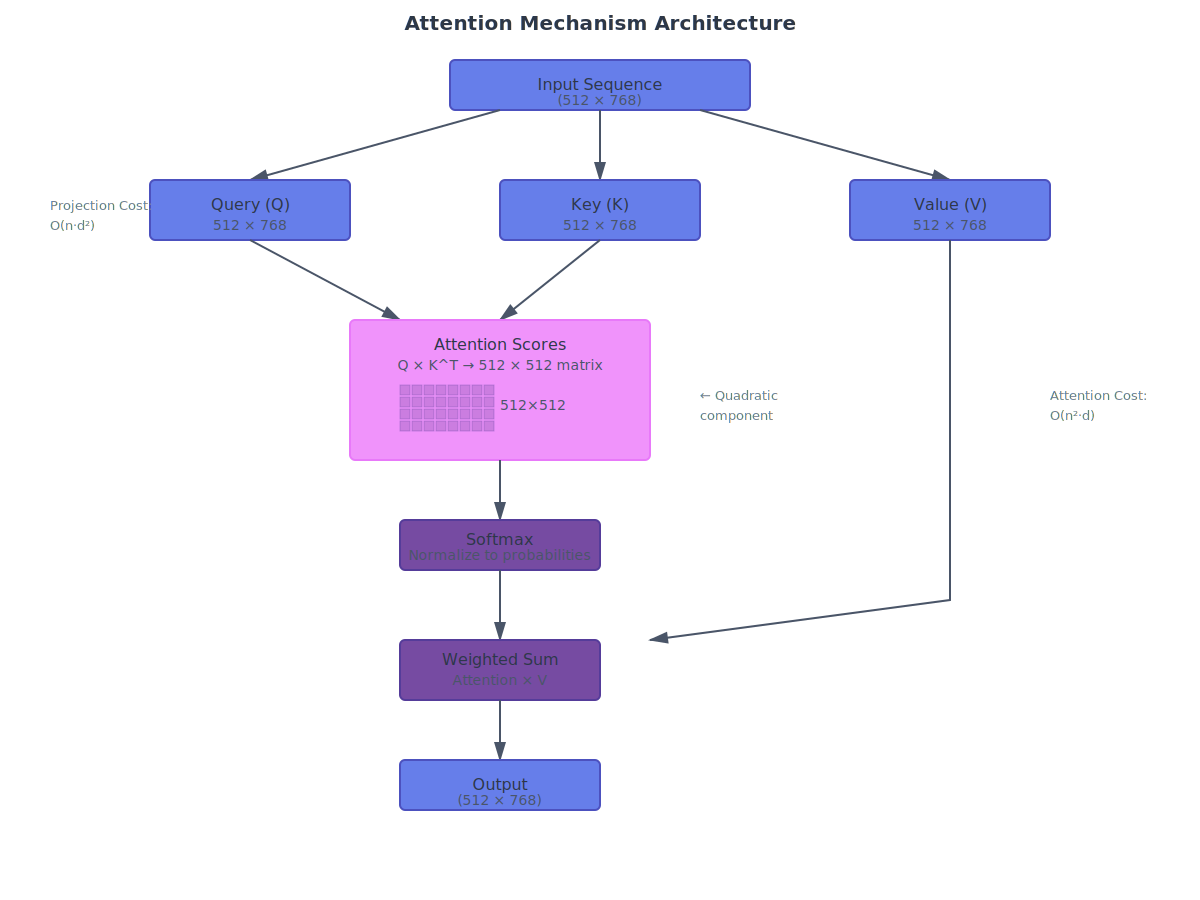
\includegraphics[width=0.95\textwidth]{chapters/diagrams/chapter03_attention_architecture_a1b2c3d4.pdf}
\caption{Attention mechanism architecture showing query-key-value projections and attention score computation. The quadratic attention matrix (n×n) drives memory and computational scaling for long sequences.}
\label{fig:attention_architecture}
\end{figure}


\section{Multi-Head Attention}

\subsection{Parallel Attention Mechanisms}

Multi-head attention employs multiple attention mechanisms in parallel, each learning different relevance patterns. BERT-base uses 12 attention heads per layer. Rather than one 768-dimensional attention mechanism, it implements 12 parallel 64-dimensional mechanisms.

The dimensional allocation: 768 dimensions divided across 12 heads yields 64 dimensions per head. Each head has its own Q, K, V projections (768×64 matrices) and produces 64-dimensional outputs. The 12 head outputs concatenate to reconstruct the full 768-dimensional representation.

This parallelization provides two benefits: diverse attention patterns (different heads learn different relevance criteria) and computational efficiency (smaller matrices enable better hardware utilization).

\subsection{Resource Implications}

Multi-head attention's resource requirements match single-head attention despite the parallelization. The total parameter count remains the same: whether implemented as one 768×768 projection or twelve 768×64 projections, the total is 768² parameters per projection type.

The computational cost similarly remains O(n·d²) for projections and O(n²·d) for attention computation. The multi-head structure reorganizes computation without changing total work.

The practical benefit: modern GPUs execute parallel operations efficiently. Twelve 64-dimensional attention computations often execute faster than one 768-dimensional computation due to better cache utilization and parallelism exploitation.

\subsection{Head Specialization}

Empirical analysis reveals that attention heads learn specialized roles. Some heads focus on syntactic relationships (subject-verb agreement), others on semantic relationships (coreference resolution), and others on positional patterns (attending to adjacent tokens).

This specialization has optimization implications. Research demonstrates that many heads contribute minimally to model performance—pruning 20-30\% of heads typically degrades accuracy by less than 1\%. For production deployments, head pruning represents a viable optimization strategy, reducing computation by 20-30\% with minimal quality impact.

\begin{figure}[htbp]
\centering
\includegraphics[width=0.9\textwidth]{chapters/diagrams/chapter03_multihead_attention_e5f6g7h8.pdf}
\caption{Multi-head attention parallel computation structure. Twelve 64-dimensional heads process independently, then concatenate. This structure enables efficient GPU utilization while learning diverse attention patterns.}
\label{fig:multihead_attention}
\end{figure}


\section{Context Length and Scaling Behavior}

\subsection{Quadratic Scaling Characteristics}

Attention's quadratic scaling with sequence length represents its most significant computational characteristic. Doubling context length quadruples attention computation and memory requirements.

For BERT-base:
\begin{itemize}
    \item 128 tokens: 128² = 16,384 attention scores per head
    \item 512 tokens: 512² = 262,144 attention scores per head (16× increase)
    \item 2048 tokens: 2048² = 4,194,304 attention scores per head (256× increase)
\end{itemize}

With 12 heads per layer and 12 layers, BERT-base computing 2048-token attention requires storing and computing approximately 600 million attention scores. At 4 bytes per score, this represents 2.4 GB of memory just for attention matrices—before considering activations, parameters, or gradients.

\subsection{Memory Bottlenecks}

For long-context applications, attention memory often becomes the limiting constraint before computational capacity. The attention matrix grows quadratically while other components grow linearly, causing attention to dominate memory consumption at sufficient length.

Memory allocation for 2048-token BERT-base processing reveals this pattern clearly. Attention matrices consume approximately 2.4 GB, representing 60\% of total memory. Other activations require approximately 1.2 GB (30\% of total), while parameters account for only 0.4 GB (10\% of total). This distribution explains why context length extensions require disproportionate memory increases.

Doubling context from 512 to 1024 tokens increases total memory requirements by approximately 3×, not 2×, due to attention's quadratic scaling. The attention matrix grows by 4× (from 512² to 1024²), while other components only double. This non-linear relationship makes memory planning for long-context applications particularly challenging.

\subsection{Practical Context Length Limits}

The quadratic scaling imposes practical limits on context length for standard attention mechanisms. On typical GPU hardware, these constraints manifest as hard memory limits that determine maximum feasible sequence lengths.

On an A100 GPU with 40 GB memory, BERT-base can process approximately 4096 tokens maximum. BERT-large, with its larger dimensional parameters, reaches its limit around 2048 tokens. At GPT-3 scale, the maximum drops to approximately 512 tokens due to the model's substantially larger parameter count and activation requirements.

These limits assume inference only. Training requires additional memory for gradients and optimizer states, reducing feasible context lengths by 2-3×. A model that can process 4096 tokens during inference might be limited to 1536 tokens during training on the same hardware.

For applications requiring longer context—document analysis, long-form generation, comprehensive code review—these constraints necessitate either architectural modifications through efficient attention variants or infrastructure investments in larger memory capacity or distributed processing across multiple GPUs.

\begin{figure}[htbp]
\centering
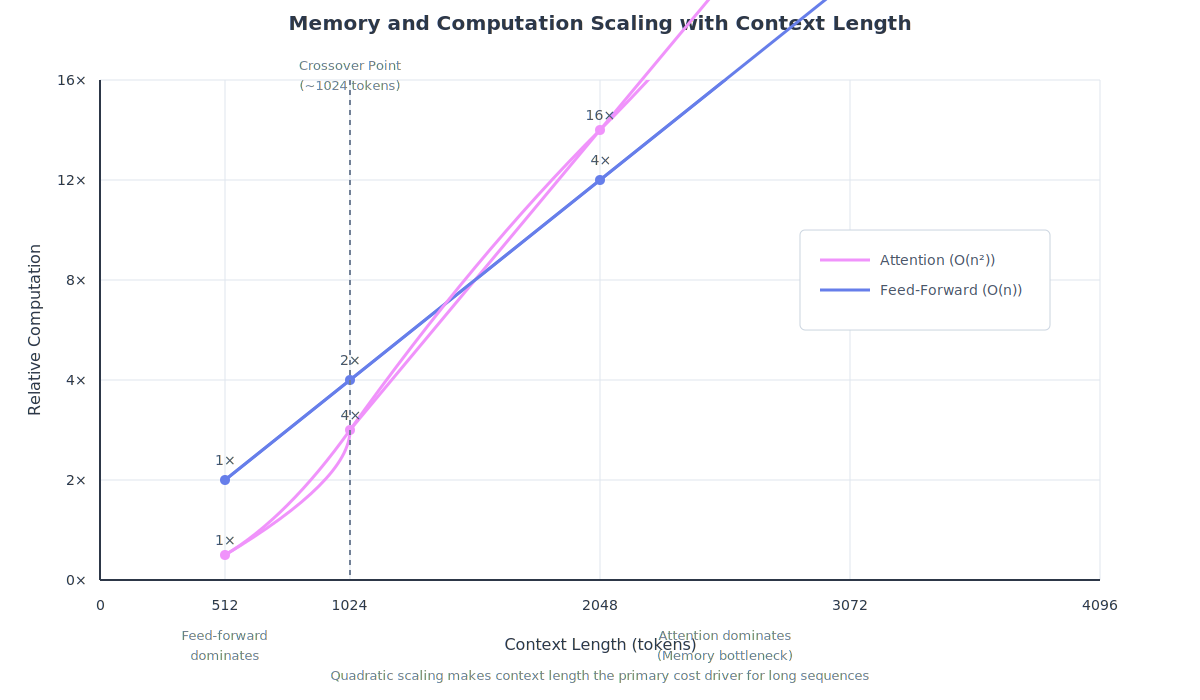
\includegraphics[width=0.9\textwidth]{chapters/diagrams/chapter03_context_scaling_i9j0k1l2.pdf}
\caption{Memory and computation scaling with context length. Attention (quadratic) dominates at longer contexts while feed-forward operations (linear) remain constant per token. The crossover point determines when context length becomes the primary cost driver.}
\label{fig:context_scaling}
\end{figure}


\section{Attention Patterns and Interpretability}

\subsection{Learned Attention Distributions}

Attention mechanisms learn which positions to emphasize through training. The resulting attention patterns provide insight into model behavior and can inform optimization decisions.

Trained models exhibit several common attention patterns. Local attention appears frequently, with many heads attending primarily to nearby tokens within approximately ±5 positions. This pattern suggests that local context often suffices for many language understanding tasks, motivating efficient attention variants that restrict attention to local windows rather than computing full quadratic attention.

Positional attention patterns emerge in some heads, which attend to specific relative positions such as the previous token or next token. These patterns are highly predictable and could potentially be hardcoded rather than learned, representing an optimization opportunity for specialized applications.

Semantic attention represents the model's long-range reasoning capability. Certain heads learn semantic relationships, attending to syntactically or semantically related tokens regardless of distance. These heads enable the model to resolve references, understand dependencies, and maintain coherence across long spans of text.

\subsection{Optimization Implications}

Understanding attention patterns enables targeted optimization strategies that trade some model expressiveness for substantial efficiency gains. The appropriate trade-off depends on application requirements and performance constraints.

Sparse attention mechanisms can skip low-weight computations when most attention weights are near-zero, as empirical analysis often reveals. This approach reduces computational work by 50-80\% with minimal accuracy impact, since the skipped computations contribute little to the final output.

Local attention windows restrict attention to fixed ranges, such as ±256 tokens, when attention is predominantly local. This restriction reduces complexity from O(n²) to O(n), enabling much longer contexts. For applications where most relevant information appears within local windows, this trade-off provides dramatic efficiency gains with acceptable accuracy.

Head pruning removes heads with minimal impact on downstream performance, reducing computation proportionally. Analysis of trained models often reveals that 20-30\% of attention heads contribute minimally to final performance, making them candidates for removal in production deployments where efficiency matters more than marginal accuracy improvements.


\section{Attention in Model Architecture}

\subsection{Attention Layers in Transformers}

Transformer architectures interleave attention layers with feed-forward layers. BERT-base's 12 layers each contain:
\begin{itemize}
    \item Multi-head attention sublayer (21M parameters, 40\% of layer computation)
    \item Feed-forward sublayer (4.7M parameters per layer, 60\% of layer computation)
\end{itemize}

Despite attention's conceptual importance, feed-forward layers consume more computation for typical sequence lengths ($\leq$512 tokens). At longer sequences, attention's quadratic scaling causes it to dominate.

The crossover point for BERT-base occurs around 1024 tokens. Below this length, feed-forward computation dominates; above it, attention dominates. This crossover point varies by model architecture and dimensional choices.

\subsection{Attention Versus Feed-Forward Trade-offs}

Model designers face trade-offs in allocating computational budget between attention and feed-forward components:

\textbf{More Attention Capacity}: Increasing attention heads or dimensions improves long-range reasoning but increases quadratic scaling costs.

\textbf{More Feed-Forward Capacity}: Increasing feed-forward dimensions improves per-token processing but doesn't enhance cross-token reasoning.

BERT-base allocates 52\% of parameters to feed-forward networks, 32\% to attention, and 16\% to embeddings. This distribution reflects empirical optimization across diverse tasks. Alternative allocations may be optimal for specific use cases (e.g., more attention for long-context tasks, more feed-forward for token-level tasks).


\section{Cost Analysis and Forecasting}

\subsection{Attention Cost Estimation}

Attention costs can be estimated using:

\begin{center}
\fbox{\parbox{0.8\textwidth}{
\centering
Attention Cost = Layers × Heads × (Projection Cost + Attention Matrix Cost)\\[0.5em]
Projection Cost = 3 × n × d²\\
Attention Matrix Cost = n² × d
}}
\end{center}

For BERT-base processing 512 tokens:
\begin{itemize}
    \item Projection: 12 layers × 12 heads × 3 × 512 × 64² $\approx$ 900M operations
    \item Attention: 12 layers × 12 heads × 512² × 64 $\approx$ 240M operations
    \item Total: $\sim$1.1B operations per forward pass
\end{itemize}

At 312 TFLOPS (A100 GPU) with 40\% efficiency: approximately 9 microseconds per forward pass for attention computation alone.

\subsection{Context Length Impact on Costs}

Context length directly impacts both latency and throughput:

\textbf{Latency}: Quadratic scaling means 4× context requires 4× more attention computation, increasing latency proportionally (assuming compute-bound).

\textbf{Throughput}: Longer contexts reduce batch sizes due to memory constraints, further reducing throughput. A 4× context increase might reduce throughput by 8-10× due to combined effects.

\textbf{Cost}: For inference-heavy applications, context length is a primary cost driver. Reducing average context length by 2× can reduce infrastructure costs by 3-4×.

\begin{tcolorbox}[colback=orange!5!white,colframe=orange!75!black,title=\textbf{MENTAL MODEL: Context Length Economic Threshold}]

\textbf{Principle:} Attention costs scale quadratically (O(n²)). Doubling context length quadruples attention cost, not doubles it.

\textbf{Economic Thresholds:}
\begin{itemize}
    \item Less than 512 tokens: Attention is cheap (less than 20\% of total cost)
    \item 512-2K tokens: Attention becomes significant (20-50\% of cost)
    \item 2K-8K tokens: Attention dominates (50-70\% of cost)
    \item Greater than 8K tokens: Consider alternatives (RAG, chunking, sparse attention)
\end{itemize}

\textbf{Decision Framework:}
\begin{enumerate}
    \item Calculate actual average context length needed (not worst-case)
    \item If greater than 4K tokens, evaluate RAG versus long-context
    \item RAG cost: (embedding + retrieval + generation with 4K context)
    \item Long-context cost: (generation with full context)
    \item Choose RAG if cost ratio exceeds 4× and quality gap is less than 5\%
\end{enumerate}

\textbf{Example:} Legal document analysis. Full contract: 50K tokens. Long-context model: (50/4)² equals 156× more expensive attention than 4K baseline. RAG approach: Chunk into 4K segments, retrieve top 3 relevant chunks, generate answer. Cost: approximately 10× cheaper with 2-3\% quality reduction.

\textbf{Red Flag:} "We need maximum context length available"—this often indicates lack of cost analysis. Question whether full context is necessary or retrieval would suffice.

\end{tcolorbox}

\subsection{Optimization ROI}

Attention optimization provides substantial returns for long-context or high-volume applications:

\textbf{Sparse Attention} (50-80\% computation reduction):
\begin{itemize}
    \item Implementation cost: 2-4 weeks engineering
    \item Accuracy impact: typically <1\%
    \item Cost savings: 50-80\% of attention computation (20-40\% of total)
\end{itemize}

\textbf{Head Pruning} (20-30\% computation reduction):
\begin{itemize}
    \item Implementation cost: 1-2 weeks analysis and validation
    \item Accuracy impact: typically <1\%
    \item Cost savings: 20-30\% of attention computation (8-15\% of total)
\end{itemize}

For systems processing millions of requests daily, these optimizations can reduce annual infrastructure costs by hundreds of thousands of dollars.


\section{Evaluation Framework}

\subsection{Attention Configuration Assessment}

When evaluating attention-related proposals, consider:

\textbf{Context Length Requirements}:
\begin{itemize}
    \item What context length is specified, and what is the justification?
    \item What percentage of inputs actually require the maximum context length?
    \item Have shorter context alternatives been evaluated?
    \item What is the memory and computational cost at the proposed context length?
\end{itemize}

\textbf{Attention Architecture}:
\begin{itemize}
    \item How many attention heads are proposed? What is the empirical justification?
    \item What is the dimensional allocation per head?
    \item Have efficient attention variants been considered (sparse, local, etc.)?
    \item What is the expected attention pattern (local, global, semantic)?
\end{itemize}

\textbf{Optimization Strategy}:
\begin{itemize}
    \item What is the plan for handling variable-length inputs efficiently?
    \item Have attention optimizations (pruning, sparsity) been evaluated?
    \item What is the memory budget, and how does attention fit within it?
    \item What is the latency target, and how does attention computation impact it?
\end{itemize}

\subsection{Common Assessment Pitfalls}

\textbf{Overspecifying Context Length}: Many applications specify maximum context length based on worst-case scenarios rather than typical usage. If 95\% of inputs use $\leq$512 tokens, optimizing for 2048-token maximum wastes resources.

\begin{tcolorbox}[colback=red!5!white,colframe=red!75!black,title=\textbf{COMMON MISTAKE: Optimizing for Maximum Context Length}]

\textbf{What Happened}:
\begin{itemize}
    \item Client requirement: "We need to handle documents up to 50,000 tokens"
    \item Team optimizes for 50k context: implements sparse attention, 6 weeks of work
    \item Actual usage distribution: 95\% of documents are <4,000 tokens
    \item 50k+ documents: <0.1\% of traffic
\end{itemize}

\textbf{Cost of mistake}: \$150,000 in engineering costs + 6 weeks delay + ongoing 3× higher infrastructure costs for edge cases

\textbf{What should have happened}:
\begin{enumerate}
    \item Analyze actual document distribution first (1 day)
    \item Optimize for the 95th percentile (4k tokens)
    \item Handle 50k+ edge cases separately (chunking, summarization, or dedicated pipeline)
    \item Total cost: \$10,000 + 1 week
\end{enumerate}

\textbf{Lesson}: Base architectural requirements on actual usage distribution, not worst-case scenarios. Measure first, optimize second.

\end{tcolorbox}

\textbf{Ignoring Quadratic Scaling}: Linear thinking about context length leads to underestimated costs. Doubling context doesn't double costs—it typically triples or quadruples them due to attention's quadratic scaling.

\textbf{Uniform Attention Assumptions}: Assuming all positions need to attend to all other positions ignores empirical attention patterns. Most applications can benefit from sparse or local attention with minimal accuracy impact.

\textbf{Neglecting Batch Size Impact}: Longer contexts reduce feasible batch sizes, compounding throughput impacts. A proposal for 4× longer context may reduce throughput by 8-10×, not 4×.

\section{Where You'll See This in Practice}

Attention mechanisms are the architectural innovation that enabled modern LLMs. Understanding their cost structure (quadratic scaling) and optimization opportunities shapes decisions across all domain applications. The following examples show how Chapter 3's concepts directly inform real-world decisions you'll face when evaluating AI proposals.

\subsection{Legal Discovery (Chapter 13.5)}

E-discovery systems processing thousands of documents face context length explosion: Depositions and contracts span 20-100 pages (50K-250K tokens). Quadratic cost impact (Section 3.3.1): 100-page document costs 25× more attention compute than 20-page document. Practical solution: Chunking plus retrieval (Chapter 5.7 RAG) versus long-context models.

\textbf{Real scenario}: Law firm evaluating document review platform. Vendor A: "We use 128K context windows to analyze full contracts." Vendor B: "We chunk documents and use RAG with 4K context." Cost analysis (using Section 3.6): Vendor A: 128K context equals (128/4)² equals 1024× more expensive attention. Vendor B: 4K context plus retrieval overhead approximately 10× cheaper. Quality: Vendor A slightly better, Vendor B "good enough" (95\% versus 97\%). Decision: Vendor B—10× cost savings justifies 2\% quality gap.

\textbf{Decision point}: When vendors tout "long context windows," ask: What's the per-document cost? Would chunking plus retrieval be more economical? Section 3.6.2 provides the calculation framework.

\subsection{Healthcare Clinical Notes (Chapter 12.2)}

Clinical NLP systems processing patient records involve multi-head attention (Section 3.2): Different heads learn symptom patterns, medication interactions, timeline relationships. Context length constraints (Section 3.3.3): Patient histories span years but models limited to 4K-8K tokens. Head specialization (Section 3.2.3): Medical terms, temporal relationships, entity recognition each use different attention heads.

\textbf{Real scenario}: Hospital implements clinical decision support. Challenge: Patient has 10-year history (500K tokens), model supports 8K tokens. Naive approach: Truncate to most recent 8K tokens, misses critical historical events. Attention-aware approach: Use retrieval to select relevant historical events based on current symptoms (Section 3.4). Result: 8K token context with curated history outperforms 32K token chronological history.

\textbf{Decision point}: Section 3.3.3's practical limits help you evaluate whether "we need longer context" or "we need smarter retrieval."

\subsection{Financial Time-Series Analysis (Chapter 14.1)}

Algorithmic trading models face temporal attention patterns (Section 3.4.1): Recent price movements weighted more heavily than historical. Multi-head specialization (Section 3.2.3): Different heads learn intraday patterns, weekly trends, earnings cycles. Latency requirements: Flash Attention (Section 3.6.3) becomes critical for microsecond trading decisions.

\textbf{Real scenario}: Hedge fund evaluating temporal fusion transformer (TFT) versus ARIMA. TFT (attention-based): Learns complex interactions, requires GPU, 10ms latency. ARIMA (statistical): Fast (1ms), interpretable, but can't capture non-linear patterns. Performance: TFT improves Sharpe ratio from 1.5 to 1.8 (20\% improvement). Decision: Deploy TFT for signals, ARIMA for risk checks (hybrid approach).

\textbf{Decision point}: Section 3.2.3's head specialization helps you understand when attention-based models justify their computational cost over simpler alternatives.

\subsection{Code Completion (Chapter 11.2)}

GitHub Copilot-style systems involve context optimization (Section 3.1.4): How much code history to include? Attention cost at scale: Millions of autocomplete requests daily. Multi-head patterns (Section 3.2.1): Different heads learn syntax, semantics, cross-file references.

\textbf{Real scenario}: Company building internal code completion tool. Challenge: Include full file (2K tokens) versus recent function (512 tokens)? Cost analysis (Section 3.3.1): 2K context costs (2000/512)² equals 15× more. Quality analysis: Full file gives 2-3\% better completions. Volume: 10M requests/day equals \$30K/day (full context) versus \$2K/day (function only). Decision: Function-only context—\$10M/year savings not justified by 2-3\% quality gain.

\textbf{Decision point}: Section 3.6.1's cost estimation framework helps you quantify the quality-cost trade-off in per-request economics.

\subsection{Semantic Search (Chapter 10.2)}

Enterprise search with RAG involves attention efficiency: Embedding models (BERT) versus generation models (GPT). Bi-directional attention (Section 3.1.2): BERT's advantage for encoding queries and documents. Cost structure: Embeddings cheap (\$0.0001/query), generation expensive (\$0.01/query).

\textbf{Real scenario}: Company deploying enterprise knowledge base search. Approach 1: Pure GPT-4—powerful but \$0.03 per query. Approach 2: BERT embeddings (\$0.0001) plus GPT-3.5 generation (\$0.002) equals \$0.0021 per query. Volume: 100K queries/month. Cost: \$3,000/month (Approach 1) versus \$210/month (Approach 2)—14× cheaper. Quality: Approach 2 slightly worse (90\% versus 94\% relevance) but acceptable.

\textbf{Decision point}: Understanding attention mechanisms (this chapter) helps you architect hybrid systems that use cheap attention (embeddings) for retrieval and expensive attention (LLMs) only for generation.

\subsection{Key Patterns: When Attention Costs Dominate}

\textbf{Attention is your bottleneck when}: Long documents (greater than 4K tokens)—costs scale quadratically (Section 3.3.1). High request volume (greater than 1M/day)—attention compute dominates total cost. Real-time requirements—efficient attention variants become critical.

\textbf{Attention costs are negligible when}: Short contexts (less than 512 tokens)—feed-forward layers dominate. Batch processing—amortize attention overhead across many examples. Low request volumes—fixed infrastructure costs dominate.

Use Section 3.6's cost analysis frameworks to determine which category your use case falls into—this determines whether attention optimization is critical or irrelevant to your budget.

\subsection{Decision Checklist: Evaluating Attention-Related Proposals}

When your team proposes attention-based architectures, verify: Context length specified and justified? (Section 3.3.3). Cost calculated for quadratic scaling with context length? (Section 3.3.1). Compared long-context versus retrieval augmentation? (Section 3.1.4). Considered efficient attention variants (Flash, sparse)? (Section 3.4.2, 6.3). Estimated per-request cost at production volume? (Section 3.6).

\textbf{Red flags}: "We need the longest context window available" (May not justify 4-16× cost increase). No mention of retrieval alternatives (Missing 10× cheaper option). Linear cost scaling assumed for context length (Ignoring quadratic reality). "Attention is cheap" with greater than 4K context (Misunderstanding of Section 3.3.1).

Chapter 3's frameworks will save you from approving architectures that work in development but become prohibitively expensive at production scale.

\section{Key Insights}

\textbf{Quadratic Scaling}: Attention computation and memory scale quadratically with sequence length. Doubling context length quadruples attention costs, making context length a primary cost driver for long-sequence applications.

\textbf{Memory Dominance}: For sequences beyond 1024 tokens, attention matrices typically consume 50-70\% of total memory. Memory constraints often limit context length before computational constraints.

\textbf{Multi-Head Benefits}: Multi-head attention provides diverse attention patterns without increasing total computation. The parallel structure also enables better hardware utilization on modern GPUs.

\textbf{Optimization Opportunities}: Most models can reduce attention computation by 50-80\% through sparse attention, head pruning, or local attention windows with minimal accuracy impact (<1\% typically).

\textbf{Context Length Trade-offs}: Maximum context length should be determined by typical usage patterns, not worst-case scenarios. Overspecifying context length wastes substantial resources due to quadratic scaling.

\textbf{Crossover Behavior}: For BERT-scale models, attention dominates computation above $\sim$1024 tokens; feed-forward layers dominate below. This crossover point informs optimization priorities.

The next chapter examines training transformers—how attention mechanisms are optimized during training, what additional memory requirements emerge, and how distributed training strategies address scale challenges.


% ============================================================================
% PART II: ARCHITECTURE LAYER (30 pages, 3 chapters)
% ============================================================================
\part{Architecture Layer}
\label{part:architecture}

% Chapter 4: Training Transformers (10 pages)
\chapter{Training Transformers at Scale}

\section*{Why This Matters}

Training transformer models represents the most significant technical and financial investment in AI system development. Understanding training infrastructure requirements, distributed training strategies, and optimization techniques is essential for accurate project planning, vendor evaluation, and infrastructure investment decisions.

The scale of transformer training has increased dramatically. GPT-2 required approximately 1,000 GPU-days; GPT-3 required 3,000-5,000 GPU-days; recent large models require tens of thousands of GPU-days. These training runs cost hundreds of thousands to millions of dollars, making training efficiency and reliability critical business concerns.

This chapter examines the technical architecture of transformer training at scale, focusing on distributed training strategies, memory optimization techniques, and the engineering trade-offs that determine training costs and timelines.

\section{Training Pipeline Architecture}

\subsection{End-to-End Training Flow}

Transformer training involves multiple coordinated stages, each with specific resource requirements and failure modes. The complete pipeline includes data loading, forward computation, backward computation, gradient aggregation, parameter updates, and checkpointing.

\textbf{Data Loading and Preprocessing}: Training data flows from storage through preprocessing pipelines to GPU memory. For large-scale training, data loading often becomes a bottleneck. A single A100 GPU can process data faster than typical storage systems can supply it, necessitating parallel data loading, prefetching, and in-memory caching.

\textbf{Forward and Backward Passes}: The model processes batches through forward computation (generating predictions) and backward computation (computing gradients). For BERT-base, a single forward-backward pass on 32 sequences requires approximately 0.6 seconds on A100 hardware. Scaling to larger models or batches increases this proportionally.

\textbf{Gradient Aggregation}: In distributed training, gradients computed across multiple GPUs must be aggregated before parameter updates. This communication step can consume 20-40\% of total training time if not optimized properly.

\textbf{Parameter Updates and Checkpointing}: After gradient aggregation, optimizers update parameters. Periodically (every 1,000-10,000 steps), the training state is checkpointed to persistent storage, enabling recovery from hardware failures.

\begin{figure}[htbp]
\centering
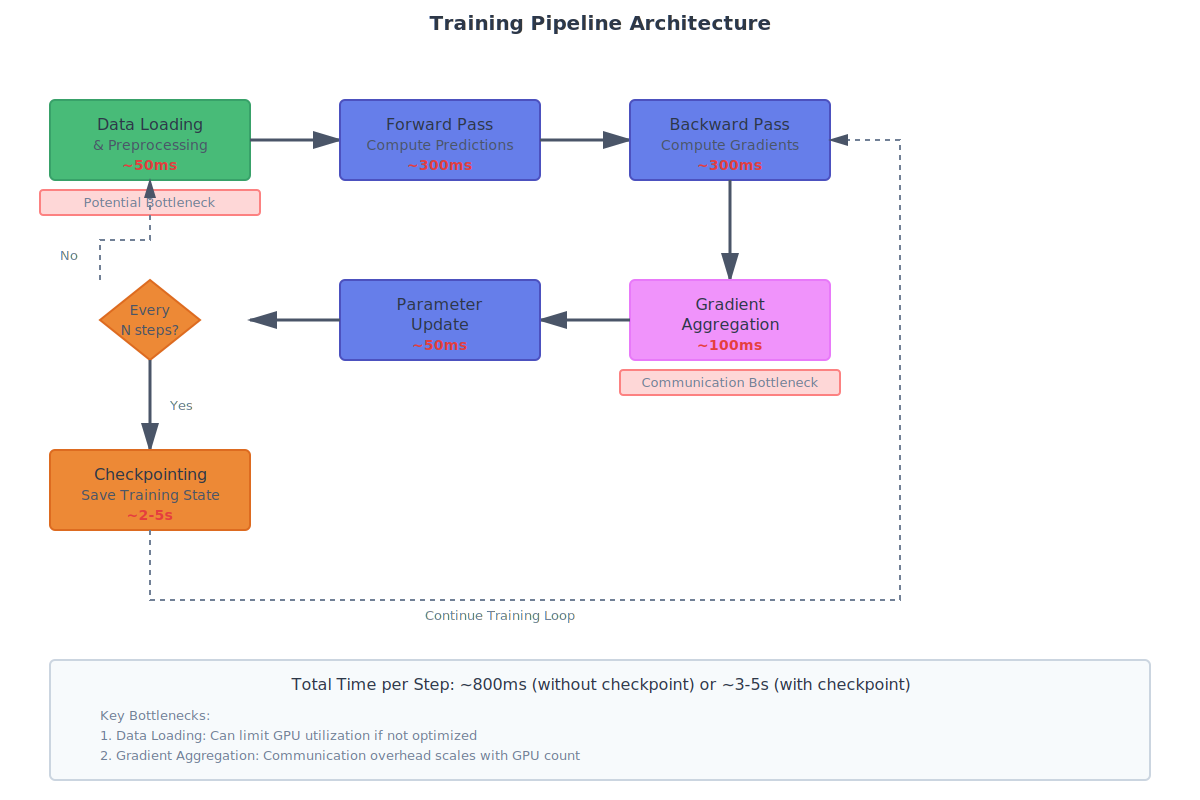
\includegraphics[width=0.95\textwidth]{chapters/diagrams/chapter04_training_pipeline_a1b2c3d4.pdf}
\caption{Complete training pipeline showing data flow, computation stages, and communication patterns. Data loading and gradient aggregation represent primary bottlenecks in distributed training.}
\label{fig:training_pipeline}
\end{figure}

\subsection{Training Time Estimation}

Training time can be estimated from model size, dataset size, and hardware specifications:

\begin{center}
\fbox{\parbox{0.85\textwidth}{
\centering
Training Time = (Parameters $\times$ Tokens $\times$ 6) / (GPU FLOPS $\times$ Utilization $\times$ GPU Count)
}}
\end{center}

The factor of 6 accounts for forward pass (1×), backward pass (2×), and additional overhead (3×). Utilization typically ranges from 30-50\% of theoretical peak performance.

For GPT-2 (1.5B parameters, 40B tokens, 8× V100 GPUs):
\begin{itemize}
    \item Computation: 1.5B $\times$ 40B $\times$ 6 = 360 $\times$ 10$^{18}$ operations
    \item GPU capacity: 8 GPUs $\times$ 125 TFLOPS $\times$ 0.4 utilization = 400 TFLOPS effective
    \item Training time: 360 $\times$ 10$^{18}$ / 400 $\times$ 10$^{12}$ = 900,000 seconds $\approx$ 250 hours $\approx$ 10 days
\end{itemize}

This matches reported GPT-2 training times, validating the estimation approach.


\section{Distributed Training Strategies}

\subsection{Data Parallelism}

Data parallelism replicates the model across multiple GPUs, with each GPU processing different data batches. This approach scales efficiently for models that fit in single-GPU memory.

\textbf{Implementation}: Each GPU maintains a complete model copy. During training, each GPU processes its batch independently, computes gradients, then all GPUs synchronize gradients through all-reduce operations. After synchronization, each GPU applies identical parameter updates.

\textbf{Scaling Characteristics}: Data parallelism scales nearly linearly up to 64-128 GPUs for large models. Beyond this point, communication overhead dominates, reducing efficiency. For BERT-base with optimized communication (NCCL 2.20+), 8-way data parallelism achieves 7.5-7.8× speedup (94-97\% efficiency); 64-way achieves 55-58× speedup (86-91\% efficiency). Older configurations achieve 75-80\% efficiency at 64-way scale.

\textbf{Memory Requirements}: Each GPU requires full model memory (parameters, gradients, optimizer states). For models exceeding single-GPU memory, data parallelism alone is insufficient.

\subsection{Model Parallelism}

Model parallelism partitions the model across multiple GPUs, enabling training of models too large for single-GPU memory. Two primary approaches exist: pipeline parallelism and tensor parallelism.

\textbf{Pipeline Parallelism}: Divides the model by layers. GPU 1 processes layers 1-4, GPU 2 processes layers 5-8, etc. Data flows through GPUs sequentially. This approach introduces pipeline bubbles—periods where GPUs idle waiting for data—reducing efficiency to 60-80\% typically.

\textbf{Tensor Parallelism}: Partitions individual layers across GPUs. A single matrix multiplication splits across multiple GPUs, which compute partial results and communicate to produce final outputs. This approach requires high-bandwidth interconnects (NVLink, InfiniBand) and achieves 80-90\% efficiency with proper implementation.

\textbf{Hybrid Approaches}: Production systems typically combine data parallelism, pipeline parallelism, and tensor parallelism. GPT-3 training used 8-way tensor parallelism, 16-way pipeline parallelism, and 8-way data parallelism, totaling 1,024 GPUs.

\begin{tcolorbox}[colback=purple!5!white,colframe=purple!75!black,title=\textbf{MENTAL MODEL: Distributed Training Decision Tree}]

\textbf{Principle:} Choose parallelism strategy based on model size and available hardware, not theoretical performance.

\textbf{Decision Framework:}

\textbf{If model fits in single GPU (less than 40GB):}
\begin{itemize}
    \item Use data parallelism only
    \item Scale to 8-64 GPUs for 7-55× speedup
    \item Efficiency: 90-95\% (minimal communication overhead)
\end{itemize}

\textbf{If model fits in single GPU but training is slow:}
\begin{itemize}
    \item Add data parallelism (2-8 GPUs)
    \item Cost: 2-8× hardware, gain: 1.9-7.5× speedup
    \item Break-even: If training takes more than 2 days, parallelism pays off
\end{itemize}

\textbf{If model exceeds single GPU (40-320GB):}
\begin{itemize}
    \item Use tensor parallelism (2-8 GPUs per model copy)
    \item Then add data parallelism across model copies
    \item Efficiency: 80-90\% (higher communication overhead)
\end{itemize}

\textbf{If model exceeds 8-GPU capacity (greater than 320GB):}
\begin{itemize}
    \item Add pipeline parallelism (layers across GPUs)
    \item Efficiency drops to 60-80\% (pipeline bubbles)
    \item Only use when necessary—complexity is high
\end{itemize}

\textbf{Example:} BERT-base (440MB parameters, 6GB training memory). Fits in single A100 (80GB). Use data parallelism with 8 GPUs for 7.5× speedup. Training time: 10 days becomes 1.3 days. Cost: 8× hardware but 7.5× faster equals 1.07× total cost for 7.5× faster delivery.

\textbf{Red Flag:} "We'll use pipeline parallelism for faster training"—pipeline parallelism is for models that don't fit, not for speed. It's slower than data parallelism due to pipeline bubbles (60-80\% efficiency versus 90-95\%).

\end{tcolorbox}

\begin{figure}[htbp]
\centering
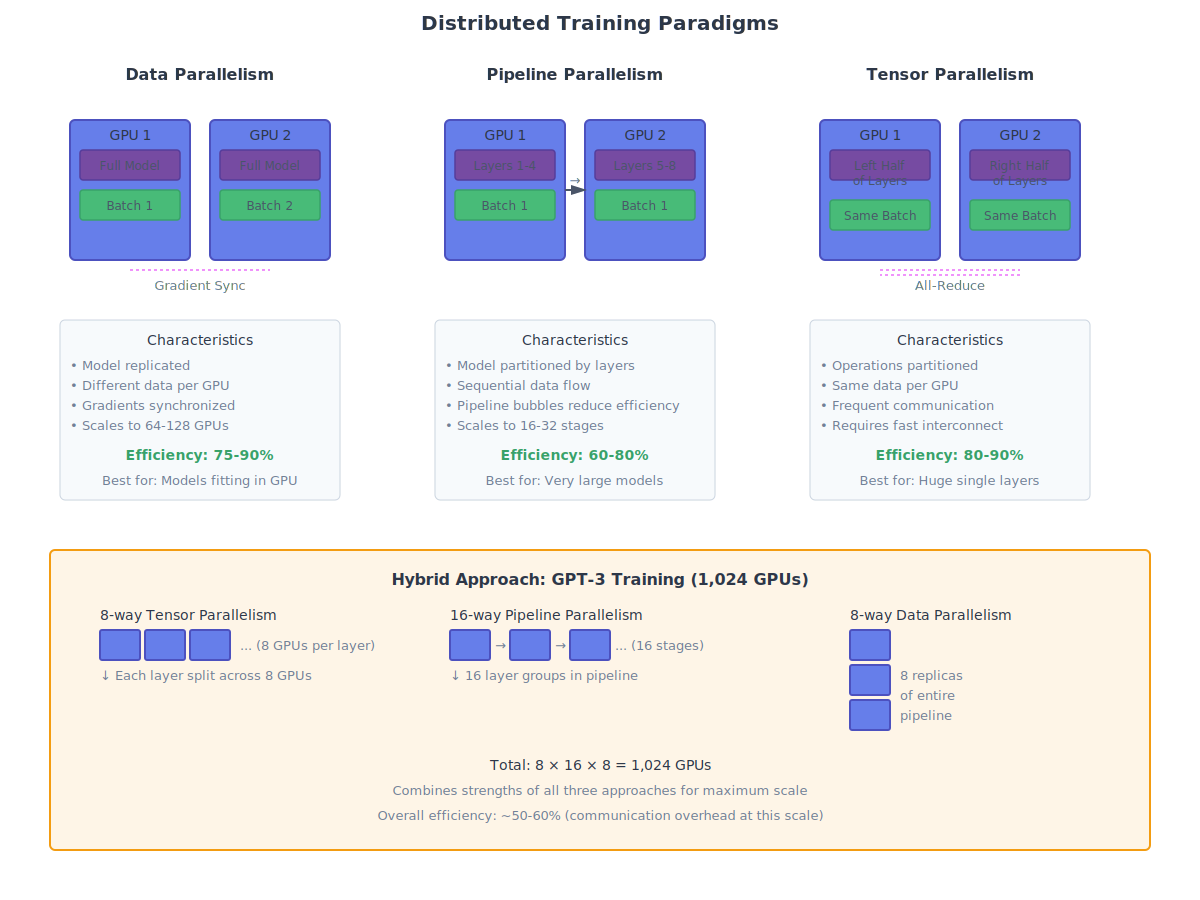
\includegraphics[width=0.9\textwidth]{chapters/diagrams/chapter04_distributed_training_e5f6g7h8.pdf}
\caption{Distributed training paradigms: data parallelism (model replication), pipeline parallelism (layer partitioning), and tensor parallelism (operation partitioning). Each approach presents different scaling characteristics and efficiency trade-offs.}
\label{fig:distributed_training}
\end{figure}

\subsection{Communication Optimization}

Distributed training efficiency depends critically on communication optimization. Gradient synchronization requires transferring gigabytes of data between GPUs, potentially consuming more time than computation.

\textbf{Gradient Accumulation}: Accumulates gradients over multiple micro-batches before synchronization, reducing communication frequency. This technique enables larger effective batch sizes without proportional memory increases.

\textbf{Mixed Precision Communication}: Communicates gradients in 16-bit precision while maintaining 32-bit precision for parameters. This halves communication volume with minimal accuracy impact.

\textbf{Gradient Compression}: Applies compression algorithms to gradients before communication. Techniques like gradient sparsification (transmitting only large gradients) can reduce communication by 100-1000× with careful tuning, though implementation complexity increases significantly.


\section{Memory Optimization Techniques}

\subsection{Activation Checkpointing}

Activation checkpointing (also called gradient checkpointing) trades computation for memory by recomputing activations during backward pass rather than storing them.

\textbf{Memory Savings}: Reduces activation memory from O(n $\times$ L) to O($\sqrt{n \times L}$), where n is batch size and L is layer count. For BERT-base, this reduces activation memory from 3.5 GB to approximately 1 GB—a 3.5× reduction.

\textbf{Computational Cost}: Increases training time by 20-33\% due to recomputation. The trade-off is favorable when memory constraints prevent training otherwise, or when larger batch sizes enabled by memory savings improve convergence sufficiently to offset recomputation costs.

\textbf{Selective Checkpointing}: Rather than checkpointing all layers, selective strategies checkpoint only expensive layers (attention layers) while storing cheap layer activations (normalization, residual connections). This approach achieves 2-2.5× memory reduction with only 10-15\% time increase.

\subsection{Mixed Precision Training}

Mixed precision training uses 16-bit floating-point (FP16) for most operations while maintaining 32-bit (FP32) precision where numerical stability requires it.

\textbf{Memory Benefits}: FP16 parameters and activations require half the memory of FP32, enabling 2× larger models or batch sizes on given hardware.

\textbf{Computational Benefits}: Modern GPUs (V100, A100, H100) include specialized FP16 hardware providing 2-8× throughput compared to FP32. For transformer training, mixed precision typically provides 1.5-2× speedup.

\textbf{Implementation Requirements}: Maintains master weights in FP32, performs forward and backward passes in FP16, then updates FP32 master weights. Loss scaling prevents gradient underflow in FP16 range. Modern frameworks (PyTorch, TensorFlow) provide automatic mixed precision, simplifying implementation.

\begin{figure}[htbp]
\centering
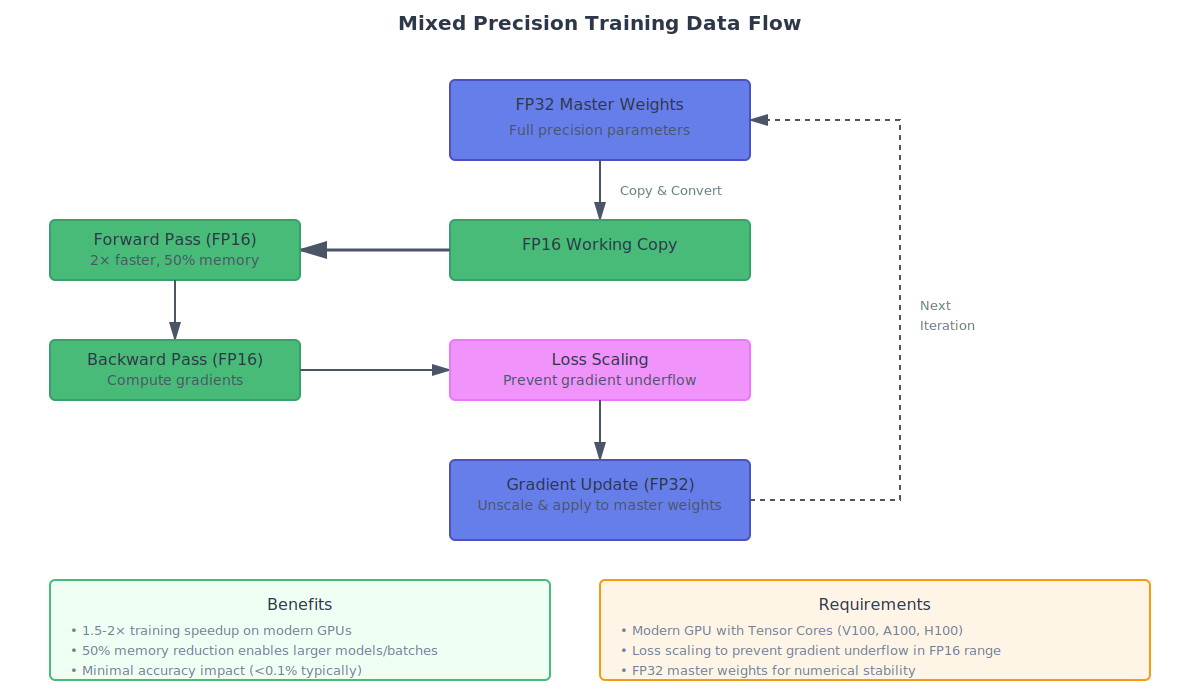
\includegraphics[width=0.9\textwidth]{chapters/diagrams/chapter04_mixed_precision_i9j0k1l2.pdf}
\caption{Mixed precision training data flow. Forward and backward passes use FP16 for speed and memory efficiency, while master weights remain in FP32 for numerical stability. Loss scaling prevents gradient underflow.}
\label{fig:mixed_precision}
\end{figure}

\subsection{Optimizer State Management}

Optimizer states (momentum, variance for Adam) consume significant memory—2× parameter memory for Adam. Several techniques reduce this overhead:

\textbf{Optimizer State Sharding}: Distributes optimizer states across GPUs rather than replicating them. Each GPU maintains optimizer states for a parameter subset, reducing per-GPU memory by GPU count. This technique, used in ZeRO optimizer, enables training models 4-8× larger on given hardware.

\textbf{8-bit Optimizers}: Quantizes optimizer states to 8-bit integers, reducing memory by 4× with minimal accuracy impact. Combined with state sharding, this enables training models 16-32× larger than naive implementations.

\textbf{CPU Offloading}: Stores optimizer states in CPU memory, transferring to GPU only during parameter updates. This trades memory for bandwidth, feasible when high-speed CPU-GPU interconnects (NVLink, PCIe 4.0) are available.


\section{Learning Rate Schedules}

\subsection{Warmup and Decay Strategies}

Learning rate schedules significantly impact training efficiency and final model quality. Transformer training typically employs warmup followed by decay.

\textbf{Linear Warmup}: Increases learning rate linearly from near-zero to target value over initial training steps. Typical warmup duration: 1-10\% of total training. This addresses optimizer initialization issues and prevents early training instability.

\textbf{Cosine Decay}: After warmup, learning rate follows cosine curve from peak to near-zero. This schedule enables aggressive exploration early and fine-tuning late, typically improving final performance by 1-3\% compared to constant learning rates.

\textbf{Inverse Square Root Decay}: Learning rate decays proportionally to $1/\sqrt{step}$. This schedule, used in original Transformer paper, provides gentler decay than cosine, sometimes preferred for very long training runs.

\begin{figure}[htbp]
\centering
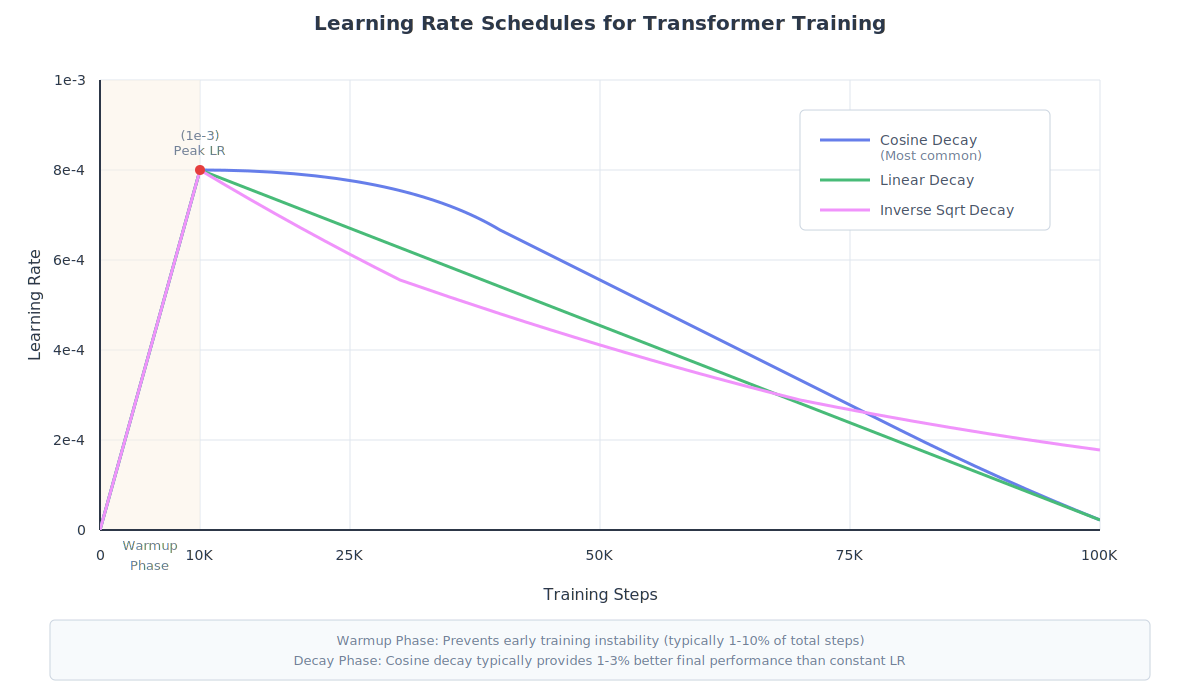
\includegraphics[width=0.9\textwidth]{chapters/diagrams/chapter04_learning_schedules_m3n4o5p6.pdf}
\caption{Common learning rate schedules for transformer training. Warmup prevents early instability; decay strategies balance exploration and convergence. Cosine decay typically provides best final performance.}
\label{fig:learning_schedules}
\end{figure}

\subsection{Adaptive Learning Rates}

Beyond scheduled decay, several techniques adapt learning rates based on training dynamics:

\textbf{Layer-wise Learning Rates}: Applies different learning rates to different layers. Early layers (closer to input) often benefit from smaller learning rates than later layers. This technique can improve convergence speed by 10-20\%.

\textbf{Gradient Clipping}: Limits gradient magnitude to prevent instability. Essential for transformer training, as attention mechanisms can produce large gradients. Typical clip values: 1.0-5.0 for gradient norm.

\textbf{Learning Rate Rewinding}: If training becomes unstable (loss spikes), rewinds to earlier checkpoint and reduces learning rate. This technique enables more aggressive initial learning rates while maintaining stability.


\section{Checkpointing and Fault Tolerance}

\subsection{Checkpoint Strategy}

Large-scale training runs span days or weeks, during which hardware failures are inevitable. Robust checkpointing is essential for training reliability.

\textbf{Checkpoint Frequency}: Balance between recovery time and checkpoint overhead. Typical strategy: checkpoint every 1,000-10,000 steps (1-4 hours of training). More frequent checkpointing reduces recovery time but increases storage I/O overhead.

\textbf{Checkpoint Content}: Full checkpoints include model parameters, optimizer states, learning rate schedule state, random number generator states, and data loader position. For BERT-base, full checkpoint size: approximately 2 GB. For GPT-3 scale: 350+ GB.

\textbf{Checkpoint Storage}: Checkpoints should be written to reliable distributed storage (not local GPU storage). Asynchronous checkpointing—writing checkpoints while training continues—prevents training interruption. This requires double-buffering checkpoint memory.

\subsection{Failure Recovery}

Hardware failures occur regularly in large-scale training. A 1,000-GPU training run experiences GPU failures approximately every 1-2 days on average.

\textbf{Automatic Recovery}: Production training systems detect failures and automatically restart from latest checkpoint. This requires orchestration systems (Kubernetes, Slurm) configured for automatic job restart.

\textbf{Partial Failure Handling}: In distributed training, single GPU failure can crash entire job. Elastic training—dynamically adjusting GPU count after failures—enables continued training with reduced resources until failed hardware is replaced.

\textbf{Checkpoint Validation}: Corrupted checkpoints can waste hours of training. Validation checks (parameter statistics, gradient norms) detect corruption before resuming training.


\section{Training Efficiency Optimization}

\subsection{Batch Size Optimization}

Batch size significantly impacts training efficiency, convergence speed, and final model quality.

\textbf{Large Batch Training}: Larger batches improve GPU utilization and reduce training time. However, very large batches can degrade final model quality. The critical batch size—beyond which larger batches don't improve convergence—varies by model and task but typically ranges from 256-2048 for transformers.

\textbf{Gradient Accumulation}: Simulates large batches without memory increase by accumulating gradients over multiple small batches before parameter updates. This enables effective batch sizes exceeding GPU memory limits.

\textbf{Batch Size Scaling}: When increasing batch size, learning rate should typically scale proportionally (linear scaling rule). Doubling batch size requires doubling learning rate to maintain convergence speed, though this rule breaks down at very large batch sizes.

\subsection{Throughput Optimization}

Maximizing training throughput—tokens processed per second—directly reduces training costs.

\textbf{Kernel Fusion}: Combines multiple operations into single GPU kernels, reducing memory traffic. Flash Attention v2, a fused attention implementation, provides 3-5× speedup for attention computation, with speedups often exceeding 5-7× for inference with context <2048 tokens. This optimization has become standard in production systems by 2025.

\textbf{Compilation Optimization}: JIT compilation (PyTorch 2.0, XLA) optimizes computation graphs, providing 10-30\% speedup with no code changes.

\textbf{Data Loading Optimization}: Ensures data loading doesn't bottleneck training. Techniques include parallel data loading, prefetching, and in-memory caching. Properly optimized data loading should consume $<$5\% of total training time.


\section{Cost Analysis and Optimization}

\subsection{Training Cost Breakdown}

Understanding cost components enables targeted optimization:

\textbf{Compute Costs} (70-80\% of total): GPU rental or amortized hardware costs. For cloud training, A100 GPUs cost approximately \$2-4/hour depending on provider and commitment level.

\textbf{Storage Costs} (10-15\% of total): Training data storage, checkpoint storage, and intermediate results. Large-scale training generates terabytes of checkpoints.

\textbf{Network Costs} (5-10\% of total): Data transfer costs, particularly for cloud training with external data sources.

\textbf{Engineering Costs} (5-10\% of total): Infrastructure setup, monitoring, debugging, and optimization. Often underestimated but significant for large-scale training.

\subsection{Cost Optimization Strategies}

Several strategies reduce training costs without compromising model quality:

\textbf{Spot Instance Usage}: Cloud spot instances cost 60-80\% less than on-demand instances. Requires robust checkpointing and automatic recovery, as spot instances can be preempted. For fault-tolerant training, spot instances can reduce costs by 50-70\%.

\textbf{Mixed Instance Types}: Uses expensive high-memory instances only where necessary, cheaper instances elsewhere. For example, use high-memory instances for parameter servers, standard instances for workers.

\textbf{Training Time Optimization}: Every 10\% reduction in training time reduces costs by 10\%. Optimizations like mixed precision, kernel fusion, and efficient data loading provide 2-3× speedup, halving training costs.

\textbf{Early Stopping}: Monitors validation metrics and stops training when improvement plateaus. Can reduce training time by 20-40\% compared to fixed-duration training.


\section{Evaluation Framework}

\subsection{Training Proposal Assessment}

When evaluating training proposals, consider:

\textbf{Resource Estimates}:
\begin{itemize}
    \item What is the estimated training time and cost? How was it calculated?
    \item What GPU type and count are specified? What is the justification?
    \item What is the expected GPU utilization? Is this realistic?
    \item What contingency is included for failures and restarts?
\end{itemize}

\textbf{Distributed Training Strategy}:
\begin{itemize}
    \item What parallelism strategy is proposed (data, pipeline, tensor)?
    \item What is the expected scaling efficiency?
    \item How will communication be optimized?
    \item What is the plan for handling hardware failures?
\end{itemize}

\textbf{Memory Optimization}:
\begin{itemize}
    \item Will activation checkpointing be used? What is the memory-time trade-off?
    \item Is mixed precision training planned? What speedup is expected?
    \item How will optimizer states be managed?
    \item What is the maximum batch size per GPU?
\end{itemize}

\textbf{Monitoring and Validation}:
\begin{itemize}
    \item What metrics will be monitored during training?
    \item What constitutes successful training completion?
    \item What is the checkpointing strategy?
    \item How will training instability be detected and addressed?
\end{itemize}

\subsection{Common Assessment Pitfalls}

\textbf{Underestimating Communication Overhead}: Distributed training proposals often assume perfect scaling. Reality: 8-GPU training achieves 7-7.5× speedup, not 8×. 64-GPU training achieves 45-50× speedup, not 64×.

\begin{tcolorbox}[colback=red!5!white,colframe=red!75!black,title=\textbf{COMMON MISTAKE: Assuming Linear Scaling in Distributed Training}]

\textbf{What Happened}:
\begin{itemize}
    \item Proposal: Train GPT-2 scale model on 64 GPUs
    \item Assumption: 64× speedup → training time = 10 days / 64 = 3.75 hours
    \item Budget: 64 GPUs × 4 hours × \$2.50/hour = \$640
    \item Reality: 55× actual speedup → training time = 4.4 hours
    \item Actual cost: \$704 (10\% over budget)
\end{itemize}

\textbf{Worse scenario} (poor communication optimization):
\begin{itemize}
    \item With older NCCL or suboptimal network: 45× speedup
    \item Training time: 5.3 hours
    \item Actual cost: \$848 (32\% over budget)
\end{itemize}

\textbf{What should have happened}:
\begin{enumerate}
    \item Assume 85\% scaling efficiency for 64 GPUs (conservative)
    \item Budget for 54× speedup, not 64×
    \item Include 15\% contingency for failures and restarts
    \item Total budget: \$850 (realistic)
\end{enumerate}

\textbf{Lesson}: Distributed training never scales perfectly. Budget for 80-90\% efficiency at scale, not 100\%.

\end{tcolorbox}

\textbf{Ignoring Failure Rates}: Large-scale training will experience failures. Proposals should include 10-20\% time contingency for failures and restarts.

\textbf{Optimistic Utilization Assumptions}: Theoretical GPU performance rarely translates to practice. Expect 30-50\% utilization, not 80-90\%.

\textbf{Inadequate Checkpointing}: Checkpoint frequency should balance recovery time against overhead. Checkpointing every 10,000 steps might seem reasonable but could mean 4-6 hours of lost work per failure.


\section{Key Insights}

\textbf{Training Dominates Costs}: Training typically consumes 80-90\% of total model development costs. Training efficiency improvements directly impact project economics.

\textbf{Distributed Training Necessity}: Models exceeding single-GPU memory require distributed training. Understanding parallelism strategies is essential for evaluating large-scale training proposals.

\textbf{Communication Bottlenecks}: For distributed training beyond 16-32 GPUs, communication often limits scaling. Proposals should explicitly address communication optimization.

\textbf{Memory-Computation Trade-offs}: Techniques like activation checkpointing and mixed precision enable training larger models or batches at the cost of increased computation. These trade-offs should be evaluated based on specific constraints.

\textbf{Failure Tolerance Required}: Hardware failures are inevitable in large-scale training. Robust checkpointing and automatic recovery are not optional—they're essential for training reliability.

\textbf{Optimization ROI}: Training efficiency improvements of 2-3× are achievable through mixed precision, kernel fusion, and data loading optimization. For million-dollar training runs, this justifies significant engineering investment.

The next chapter examines production deployment—how trained models are optimized for inference, what serving architectures enable efficient deployment, and how to evaluate deployment costs and performance.


% Chapter 5: Production Deployment (10 pages)
\chapter{Production Deployment and Inference Optimization}

\section*{Why This Matters}

Production deployment represents the operational phase where models deliver business value. While training is a one-time investment, inference costs are ongoing operational expenses that scale with usage. For high-volume applications serving millions of requests daily, inference costs can exceed training costs within weeks or months.

Understanding inference optimization techniques, serving architectures, and deployment trade-offs is essential for accurate cost forecasting, infrastructure planning, and vendor evaluation. A model that costs \$50,000 to train might cost \$500,000 annually to serve at scale—making deployment efficiency a primary economic concern.

This chapter examines production deployment from an engineering and economic perspective, focusing on optimization techniques, serving architectures, and the trade-offs that determine deployment costs and performance.

\section{Inference Versus Training Requirements}

\subsection{Resource Profile Differences}

Inference and training present fundamentally different resource requirements and optimization opportunities.

\textbf{Memory Requirements}: Inference eliminates gradients, optimizer states, and large activation batches required for training. BERT-base requires approximately 6 GB for training but only 500 MB for inference—a 12× reduction. This disparity enables deployment on less expensive hardware or higher throughput on given hardware.

\textbf{Computational Patterns}: Training performs forward and backward passes; inference performs only forward passes. This halves computational requirements per input. Additionally, inference typically processes smaller batches (1-32 sequences) versus training batches (32-512 sequences), changing memory access patterns and optimization opportunities.

\textbf{Latency Sensitivity}: Training tolerates variable latency—a batch taking 0.5 seconds versus 0.6 seconds rarely matters. Inference often requires strict latency guarantees—99th percentile latency under 100ms for interactive applications. This constraint shapes optimization strategies and infrastructure choices.

\subsection{Optimization Priorities}

Training optimization prioritizes throughput—maximizing tokens processed per dollar. Inference optimization balances multiple objectives:

\textbf{Latency}: Time from request to response. Critical for interactive applications (chatbots, search). Target latencies range from 50ms (search) to 500ms (content generation).

\textbf{Throughput}: Requests processed per second per server. Determines infrastructure costs for high-volume applications.

\textbf{Cost}: Infrastructure expenses per million requests. Combines hardware costs, utilization rates, and operational overhead.

These objectives often conflict. Optimizing for minimum latency (small batches, dedicated hardware) increases cost per request. Optimizing for minimum cost (large batches, shared hardware) increases latency. Production deployments navigate these trade-offs based on application requirements.


\section{Model Compression Techniques}

\subsection{Quantization}

Quantization reduces numerical precision from 32-bit or 16-bit floating-point to 8-bit integers, decreasing model size and increasing inference speed.

\textbf{Post-Training Quantization}: Converts trained model weights to lower precision without retraining. For BERT-base, 8-bit quantization reduces model size from 440 MB to 110 MB (4× reduction) with typically $<$1\% accuracy degradation. Implementation requires calibration on representative data to determine optimal quantization parameters.

\textbf{Quantization-Aware Training}: Simulates quantization during training, enabling the model to adapt to reduced precision. This approach achieves better accuracy than post-training quantization, often maintaining full precision performance while using 8-bit inference.

\textbf{Performance Benefits}: Modern CPUs and GPUs include specialized 8-bit arithmetic instructions providing 2-4× throughput compared to 32-bit operations. For BERT-base on CPU, quantization typically provides 3× speedup with 4× memory reduction.

\subsection{Knowledge Distillation}

Knowledge distillation trains a smaller "student" model to replicate a larger "teacher" model's behavior, achieving comparable performance with fewer parameters.

\textbf{Distillation Process}: The student model trains on both ground-truth labels and teacher model predictions. Teacher predictions provide richer training signal than labels alone, enabling smaller models to achieve higher accuracy than training from scratch.

\textbf{Typical Results}: DistilBERT (66M parameters) achieves 97\% of BERT-base (110M parameters) performance with 40\% fewer parameters and 60\% faster inference. For production deployment, this translates to 40\% lower infrastructure costs with minimal quality degradation.

\textbf{Implementation Considerations}: Distillation requires access to teacher model during student training, increasing training costs. However, for high-volume applications, deployment savings justify distillation investment within days or weeks.

\subsection{Pruning}

Pruning removes parameters with minimal impact on model performance, reducing model size and computational requirements.

\textbf{Unstructured Pruning}: Removes individual weights based on magnitude or importance metrics. Can achieve 50-80\% sparsity (parameter removal) with $<$1\% accuracy loss. However, unstructured sparsity provides limited speedup on standard hardware without specialized sparse computation libraries.

\textbf{Structured Pruning}: Removes entire neurons, attention heads, or layers, producing models that run efficiently on standard hardware. Typical results: 30-40\% parameter reduction with 1-2\% accuracy loss and proportional speedup.

\textbf{Practical Application}: Structured pruning is more practical for production deployment due to hardware compatibility. Removing 4 of 12 attention heads reduces computation by 33\% with minimal accuracy impact, requiring no specialized hardware or libraries.

\begin{figure}[htbp]
\centering
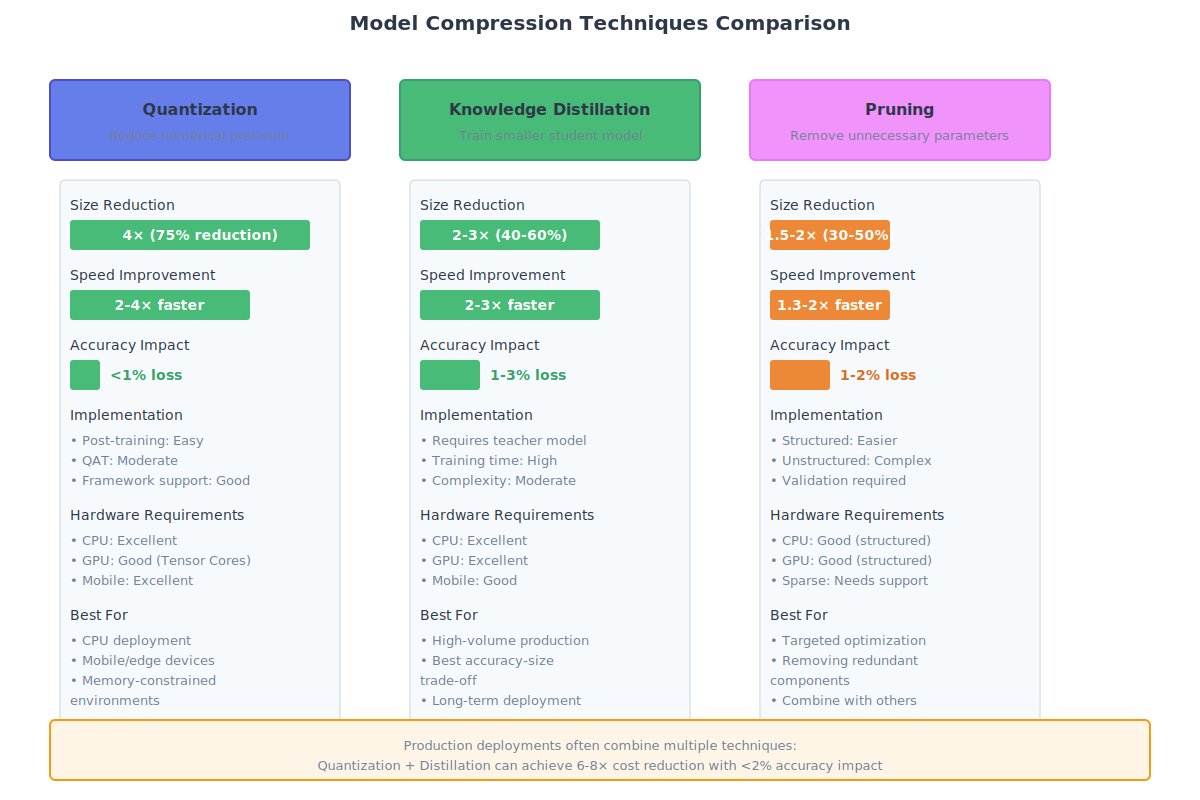
\includegraphics[width=0.95\textwidth]{chapters/diagrams/chapter05_compression_comparison_a1b2c3d4.pdf}
\caption{Model compression techniques comparison. Quantization provides best speed-memory trade-off; distillation provides best accuracy-size trade-off; pruning enables targeted optimization. Production deployments often combine multiple techniques.}
\label{fig:compression_comparison}
\end{figure}

\begin{tcolorbox}[colback=cyan!5!white,colframe=cyan!75!black,title=\textbf{MENTAL MODEL: Compression-Quality Frontier}]

\textbf{Principle:} Most models can be compressed 2-4× with less than 1\% accuracy loss. Beyond that, quality degrades rapidly.

\textbf{The Compression Ladder:}

\textbf{Level 1 (2× compression, less than 0.5\% accuracy loss):}
\begin{itemize}
    \item INT8 quantization (post-training)
    \item Effort: 1-2 days, Cost: \$0
    \item Use: Always—no reason not to
\end{itemize}

\textbf{Level 2 (3-4× compression, less than 1\% accuracy loss):}
\begin{itemize}
    \item Knowledge distillation (train smaller model)
    \item Effort: 1-2 weeks, Cost: \$2K-5K
    \item Use: When serving greater than 10M requests/month
\end{itemize}

\textbf{Level 3 (4-8× compression, 1-3\% accuracy loss):}
\begin{itemize}
    \item Aggressive pruning plus quantization
    \item Effort: 2-4 weeks, Cost: \$5K-10K
    \item Use: When cost savings (greater than \$50K/year) justify quality trade-off
\end{itemize}

\textbf{Level 4 (greater than 8× compression, greater than 3\% accuracy loss):}
\begin{itemize}
    \item Extreme compression (4-bit quantization, 90\% pruning)
    \item Effort: 1-2 months, Cost: \$10K-20K
    \item Use: Rarely—usually better to redesign architecture
\end{itemize}

\textbf{Decision Framework:}
\begin{enumerate}
    \item Start with Level 1 (INT8)—always worth it
    \item Calculate annual inference cost at current volume
    \item If greater than \$100K/year, invest in Level 2 (distillation)
    \item If greater than \$500K/year and 1-3\% quality loss acceptable, consider Level 3
    \item Never go to Level 4—redesign instead
\end{enumerate}

\textbf{Example:} Serving 50M requests/month at \$0.002/request equals \$100K/month equals \$1.2M/year. Level 2 compression (3× reduction) saves \$800K/year. Investment: \$5K. ROI: 160× in year 1.

\textbf{Red Flag:} "We need 10× compression"—this usually indicates wrong model choice. A properly-sized model with 2-4× compression beats an oversized model with 10× compression.

\end{tcolorbox}

\section{Inference Optimization Techniques}

\subsection{Operator Fusion}

Operator fusion combines multiple operations into single optimized kernels, reducing memory traffic and improving performance.

\textbf{Attention Fusion}: Standard attention implementation performs query-key multiplication, softmax, and attention-value multiplication as separate operations. Fused attention (Flash Attention, xFormers) combines these into a single kernel, reducing memory traffic by 3-4× and providing 2-4× speedup.

\textbf{Layer Fusion}: Combines layer normalization, activation functions, and residual connections into fused operations. For transformer layers, fusion typically provides 10-20\% speedup with no accuracy impact.

\textbf{Framework Support}: Modern frameworks (PyTorch 2.0, TensorFlow, ONNX Runtime) provide automatic fusion through compilation. Manual fusion using custom CUDA kernels can provide additional 20-30\% speedup but requires significant engineering investment.

\subsection{Batching Strategies}

Batching—processing multiple requests together—improves GPU utilization and throughput but increases latency.

\textbf{Static Batching}: Accumulates requests until batch size threshold is reached or timeout expires, then processes batch. Simple to implement but introduces latency variance. For batch size 32 with 100ms timeout, average latency increases by 50ms compared to single-request processing.

\textbf{Dynamic Batching}: Continuously processes available requests in variable-size batches, balancing latency and throughput. More complex to implement but provides better latency-throughput trade-off. Typical configuration: maximum batch size 32, maximum wait time 10ms.

\textbf{Continuous Batching}: Processes requests as they arrive without waiting for batch completion, enabling lower latency with high throughput. Requires careful memory management and scheduling but provides optimal latency-throughput balance for variable-length inputs.

\subsection{KV Cache Optimization}

For autoregressive generation (text generation, translation), key-value (KV) cache optimization significantly improves performance and represents one of the highest-ROI production optimizations.

\textbf{KV Cache Mechanism}: During generation, attention keys and values from previous tokens are cached and reused, avoiding recomputation. For a 512-token generation, KV caching reduces computation by approximately 500× compared to recomputing from scratch each step.

\textbf{Memory Requirements}: KV cache memory scales with sequence length and batch size. For BERT-base generating 512 tokens with batch size 8, KV cache requires approximately 2 GB. This memory overhead limits batch sizes for long-sequence generation.

\textbf{Multi-Query Attention (MQA) and Grouped-Query Attention (GQA)}: By 2026, these techniques have become standard for production inference, not optional optimizations. They reduce KV cache by 4-8× with <1\% quality degradation:

For LLaMA 2 scale models:
\begin{itemize}
    \item Standard attention: 1.6 GB KV cache per batch of 32
    \item GQA (8 groups): 200 MB KV cache
    \item Impact: 40-80\% inference throughput improvement on memory-bound workloads
\end{itemize}

These should be default choices for production inference, not optimization afterthoughts. The memory savings enable larger batch sizes, directly improving throughput and reducing per-request costs.

\textbf{PagedAttention}: Recent optimization technique that manages KV cache memory more efficiently through paging, similar to virtual memory in operating systems. This approach increases achievable batch size by 2-3× for long-sequence generation, proportionally improving throughput. Combined with GQA, PagedAttention enables 6-10× throughput improvements for long-context generation.


\section{Serving Architectures}

\subsection{Model Serving Patterns}

Production deployments employ various serving patterns based on latency requirements, throughput needs, and cost constraints.

\textbf{Dedicated Model Servers}: Each model runs on dedicated hardware with isolated resources. This pattern provides predictable latency and simplifies capacity planning but increases costs for multiple models. Appropriate for high-volume, latency-sensitive applications.

\textbf{Multi-Model Serving}: Multiple models share hardware resources, improving utilization and reducing costs. Requires careful resource allocation and scheduling to prevent interference. Appropriate for lower-volume models or when latency requirements are relaxed.

\textbf{Serverless Deployment}: Models deployed as serverless functions that scale automatically with demand. Provides excellent cost efficiency for variable or unpredictable load but introduces cold-start latency (1-5 seconds typically). Appropriate for batch processing or asynchronous workflows.

\begin{figure}[htbp]
\centering
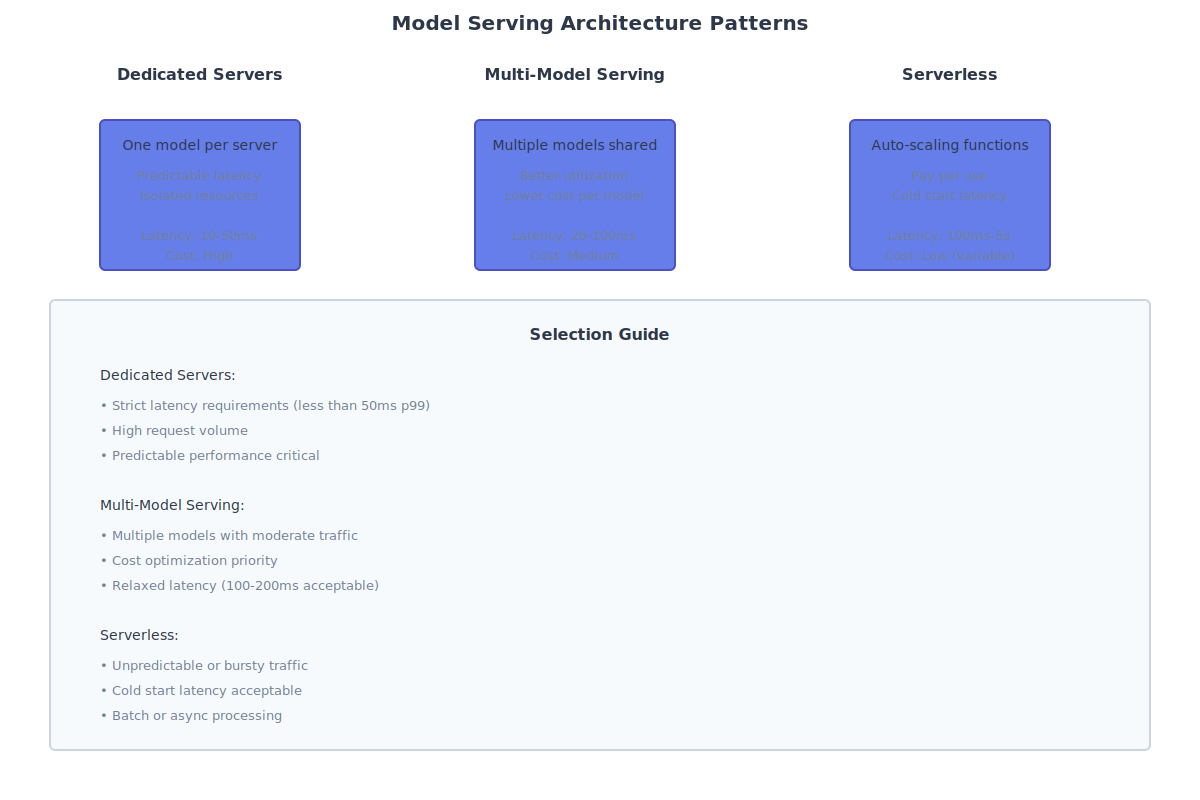
\includegraphics[width=0.9\textwidth]{chapters/diagrams/chapter05_serving_architecture_e5f6g7h8.pdf}
\caption{Model serving architecture patterns. Dedicated servers provide lowest latency; multi-model serving provides best resource utilization; serverless provides best cost efficiency for variable load. Choice depends on latency requirements and usage patterns.}
\label{fig:serving_architecture}
\end{figure}

\subsection{Load Balancing and Scaling}

Effective load balancing and scaling strategies ensure consistent performance under variable load.

\textbf{Horizontal Scaling}: Adds more model server instances to handle increased load. Provides linear scaling for stateless inference but requires load balancer and health monitoring. Typical scaling policy: add instance when CPU utilization exceeds 70\%, remove when below 30\%.

\textbf{Vertical Scaling}: Uses larger instances with more GPUs or memory. Simpler than horizontal scaling but limited by maximum instance size. Appropriate when single-instance performance is insufficient.

\textbf{Auto-Scaling}: Automatically adjusts instance count based on metrics (request rate, latency, utilization). Essential for variable load patterns. Typical configuration: scale up aggressively (30-60 seconds), scale down conservatively (5-10 minutes) to prevent oscillation.

\subsection{Caching Strategies}

Caching reduces inference costs by storing and reusing results for repeated requests.

\textbf{Result Caching}: Caches complete inference results keyed by input. Highly effective for repeated queries (FAQ systems, common searches). Cache hit rates of 30-50\% are common, reducing infrastructure costs proportionally.

\textbf{Embedding Caching}: Caches intermediate representations (embeddings) for frequently-accessed content. Useful for retrieval systems where document embeddings are computed once and reused for multiple queries.

\textbf{Cache Invalidation}: Determines when cached results become stale. Simple time-based expiration (TTL) works for most applications. More sophisticated approaches track model version and invalidate on updates.


\section{Deployment Platforms and Trade-offs}

\subsection{Cloud Deployment}

Cloud platforms (AWS, GCP, Azure) provide managed infrastructure with flexible scaling but introduce ongoing costs.

\textbf{Managed Services}: Platforms like AWS SageMaker, GCP Vertex AI, Azure ML provide fully-managed model serving with automatic scaling, monitoring, and updates. Simplifies operations but costs 20-40\% more than self-managed infrastructure.

\textbf{Container-Based Deployment}: Deploy models in containers (Docker, Kubernetes) on cloud VMs. Provides flexibility and cost efficiency but requires more operational expertise. Typical cost: \$2-4/hour for GPU instances (A100), \$0.10-0.30/hour for CPU instances.

\textbf{Spot Instances}: Use preemptible instances at 60-80\% discount for fault-tolerant workloads. Requires graceful handling of instance termination. Appropriate for batch processing or when redundancy enables tolerance of individual instance failures.

\subsection{On-Premises Deployment}

On-premises deployment provides control and potentially lower long-term costs but requires capital investment and operational expertise.

\textbf{Capital Costs}: GPU servers cost \$50,000-150,000 depending on configuration (A100 servers typically \$100,000-120,000). Amortized over 3-year lifetime: approximately \$3,000-4,000/month per server.

\textbf{Operational Costs}: Power, cooling, networking, and maintenance add 30-50\% to hardware costs. A 10-server GPU cluster costs approximately \$40,000-60,000/month including all operational expenses.

\textbf{Break-Even Analysis}: On-premises deployment becomes cost-effective at sufficient scale. For continuous GPU utilization, break-even typically occurs at 6-12 months compared to cloud deployment. For variable utilization, cloud deployment often remains more cost-effective.

\subsection{Edge Deployment}

Edge deployment runs models on user devices or edge servers, reducing latency and cloud costs but constraining model size.

\textbf{Mobile Deployment}: Models run on smartphones or tablets. Requires aggressive compression (quantization, distillation) to fit memory constraints (typically $<$100 MB) and power constraints. Appropriate for privacy-sensitive applications or offline functionality.

\textbf{Edge Servers}: Deploy models on edge servers closer to users, reducing latency from 100-200ms (cloud) to 10-30ms (edge). Requires distributed deployment and management but provides better user experience for latency-sensitive applications.

\textbf{Hybrid Approaches}: Combine edge and cloud deployment, running small models on-device for common cases and falling back to cloud for complex cases. Balances latency, cost, and capability.

\begin{figure}[htbp]
\centering
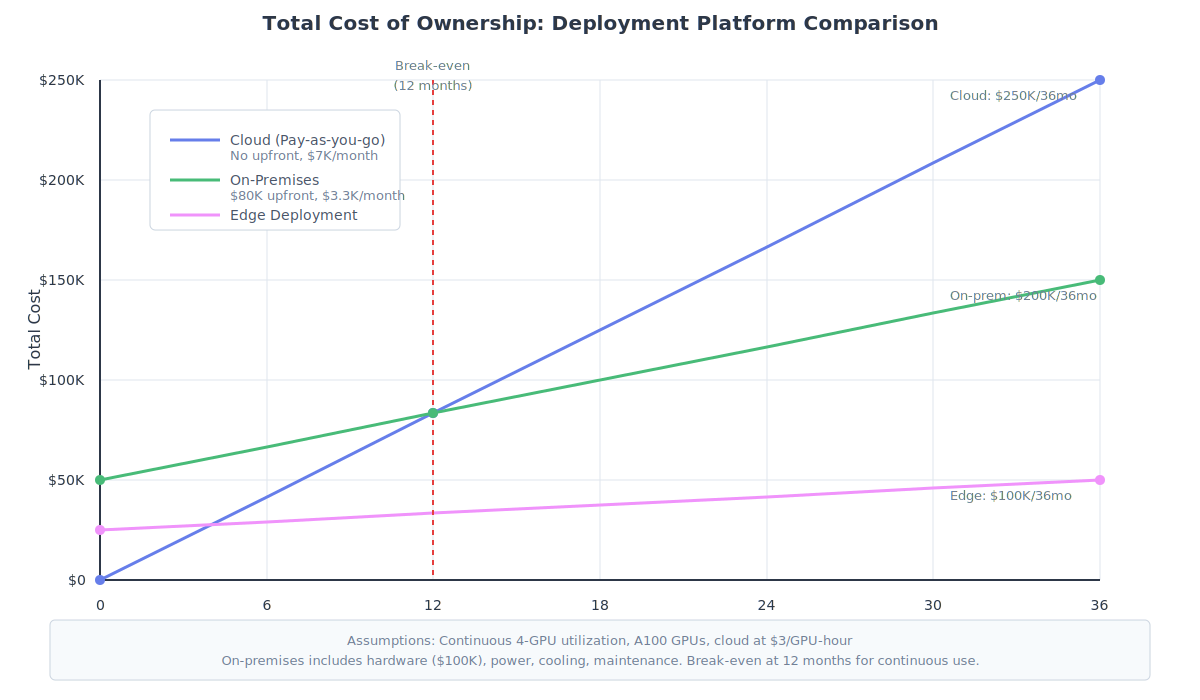
\includegraphics[width=0.9\textwidth]{chapters/diagrams/chapter05_deployment_costs_i9j0k1l2.pdf}
\caption{Deployment cost comparison across platforms. Cloud provides flexibility; on-premises provides lower long-term costs at scale; edge provides lowest latency and ongoing costs. Choice depends on scale, utilization patterns, and latency requirements.}
\label{fig:deployment_costs}
\end{figure}


\section{Cost Analysis and Optimization}

\subsection{Inference Cost Breakdown}

Understanding cost components enables targeted optimization:

\textbf{Compute Costs} (60-70\%): GPU or CPU rental/amortization. For cloud deployment with A100 GPUs at \$3/hour, processing 1 million BERT-base requests (50ms each) costs approximately \$42 in compute time.

\textbf{Memory and Storage} (10-15\%): Model storage, KV cache memory, and intermediate results. Larger models or longer sequences increase memory costs proportionally.

\textbf{Network Costs} (10-15\%): Data transfer between services and to users. For cloud deployment, egress costs can be significant—typically \$0.08-0.12/GB.

\textbf{Operational Overhead} (10-15\%): Monitoring, logging, load balancing, and management infrastructure. Often underestimated but essential for production reliability.

\subsection{Cost Optimization Strategies}

Several strategies reduce inference costs without compromising quality:

\textbf{Model Compression}: Quantization and distillation reduce costs by 2-4× with minimal accuracy impact. For a system serving 100 million requests monthly at \$0.001/request, compression reduces costs from \$100,000 to \$25,000-50,000 monthly.

\begin{tcolorbox}[colback=blue!5!white,colframe=blue!75!black,title=\textbf{IN PRACTICE: ROI of Model Compression}]

\textbf{Scenario}: E-commerce company serving 100M product recommendations/month

\textbf{Before Compression} (BERT-base, FP32):
\begin{itemize}
    \item Model size: 440 MB
    \item Latency: 50ms per request
    \item Infrastructure: 20× A100 GPUs
    \item Monthly cost: \$100,000
\end{itemize}

\textbf{After Compression} (8-bit quantization + distillation):
\begin{itemize}
    \item Model size: 110 MB (4× reduction)
    \item Latency: 18ms per request (2.8× faster)
    \item Infrastructure: 8× A100 GPUs (60\% reduction)
    \item Monthly cost: \$40,000
    \item Accuracy impact: -0.3\% (negligible)
\end{itemize}

\textbf{Investment vs. Return}:
\begin{itemize}
    \item Engineering cost: 2 weeks × \$10k/week = \$20,000
    \item Monthly savings: \$60,000
    \item Payback period: 10 days
    \item Annual savings: \$720,000
\end{itemize}

\textbf{Lesson}: For high-volume applications, compression engineering pays for itself within days.

\end{tcolorbox}

\textbf{Batching Optimization}: Increasing batch size from 1 to 16 typically improves throughput by 8-12×, reducing per-request costs proportionally. Requires balancing against latency requirements.

\textbf{Hardware Selection}: CPU inference costs 5-10× less than GPU inference for small models or low throughput. For BERT-base with $<$10 requests/second, CPU deployment is more cost-effective. Above 50 requests/second, GPU deployment becomes more economical.

\textbf{Caching}: Result caching with 30\% hit rate reduces infrastructure costs by 30\%. Implementation cost is minimal—typically a Redis or Memcached cluster costing $<$5\% of inference infrastructure.

\subsection{Cost Forecasting}

Accurate cost forecasting requires understanding scaling relationships:

\begin{center}
\fbox{\parbox{0.85\textwidth}{
\centering
Monthly Cost = (Requests/Month) $\times$ (Latency/Request) $\times$ (GPU Cost/Hour) / (3600 $\times$ Batch Size $\times$ Utilization)
}}
\end{center}

For 100 million monthly requests, 50ms latency, \$3/hour GPU cost, batch size 16, 60\% utilization:

Monthly Cost = 100M $\times$ 0.05 $\times$ 3 / (3600 $\times$ 16 $\times$ 0.6) $\approx$ \$43,000

This formula enables rapid cost estimation for different scenarios and optimization strategies.


\section{Retrieval-Augmented Generation (RAG)}

\subsection{RAG Architecture}

RAG combines retrieval systems with generative models, enabling models to access external knowledge without retraining. This fundamentally changes the cost structure of LLM applications.

\textbf{Architecture Components}: RAG systems include a retrieval component (vector database, search engine) and a generation component (language model). User queries trigger retrieval of relevant documents, which are provided as context to the language model for generation.

\textbf{Benefits}: RAG enables models to access current information, cite sources, and reduce hallucination. For enterprise applications, RAG provides access to proprietary knowledge without expensive model retraining. RAG also enables dynamic knowledge updates without retraining—a critical advantage for rapidly-changing domains.

\textbf{Cost Implications and Economics}: RAG adds retrieval costs (vector database queries, embedding computation) to generation costs. However, RAG often enables use of smaller language models since external knowledge reduces model size requirements.

For 1M queries/month:
\begin{itemize}
    \item Base LLM cost (7B model): \$3,000-5,000
    \item Retrieval cost (embedding model + vector DB): \$500-2,000
    \item Total monthly: \$3,500-7,000
    \item vs. Fine-tuned equivalent (70B model): \$30,000-50,000
\end{itemize}

RAG enables 4-7× cost reduction compared to larger models for comparable performance. Net cost impact varies by application but is often neutral or positive when accounting for the ability to use smaller base models.

\subsection{Implementation Considerations}

Effective RAG implementation requires attention to several technical details:

\textbf{Retrieval Quality}: Retrieval accuracy directly impacts generation quality. Poor retrieval provides irrelevant context, degrading output quality. Typical approach: retrieve top-k documents (k=3-10), rerank using cross-encoder, provide top-3 to generator.

\textbf{Context Length Management}: Retrieved documents must fit within model context window. For models with 2048-token context, retrieved content typically limited to 1000-1500 tokens, leaving room for query and generation.

\textbf{Latency Considerations}: RAG adds retrieval latency (typically 20-50ms) to generation latency. For latency-sensitive applications, this overhead requires optimization through caching, parallel retrieval, or approximate search.

\begin{figure}[htbp]
\centering
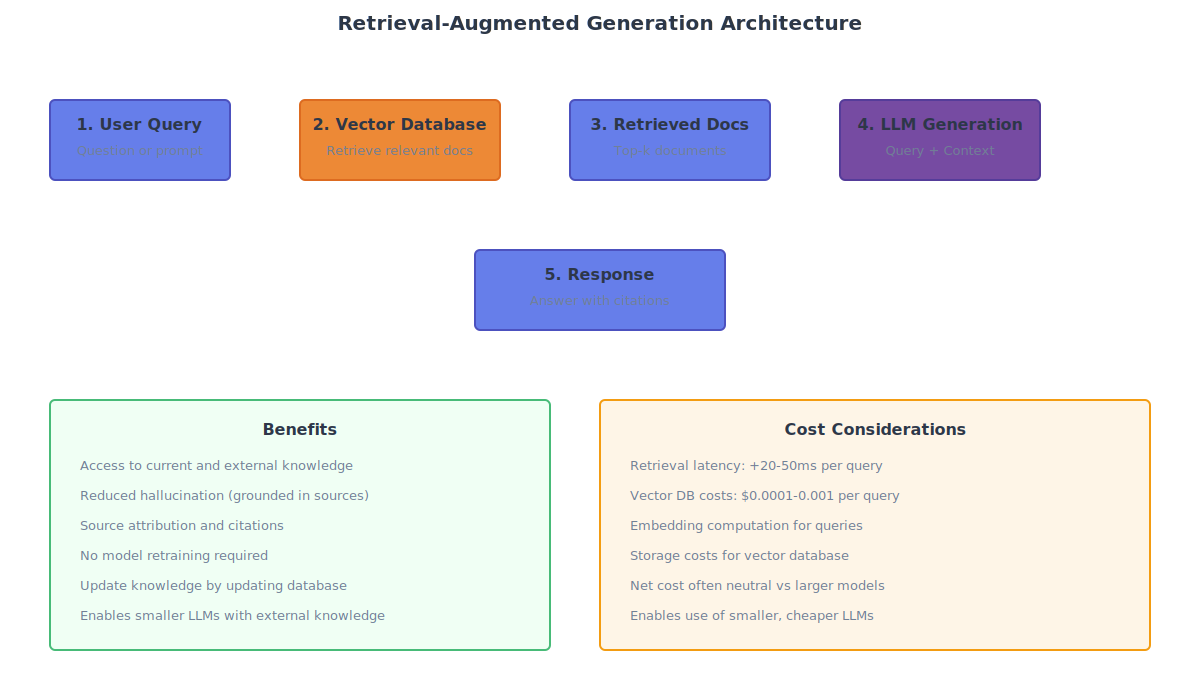
\includegraphics[width=0.95\textwidth]{chapters/diagrams/chapter05_rag_architecture_m3n4o5p6.pdf}
\caption{Retrieval-Augmented Generation architecture. User query triggers document retrieval from vector database, retrieved documents provide context for language model generation. This architecture enables access to external knowledge without model retraining.}
\label{fig:rag_architecture}
\end{figure}


\section{Monitoring and Observability}

\subsection{Performance Metrics}

Production deployments require comprehensive monitoring to ensure reliability and performance:

\textbf{Latency Metrics}: Track p50, p95, p99 latency. p99 latency (99th percentile) is critical for user experience—1\% of users experiencing 10× higher latency is unacceptable for most applications.

\textbf{Throughput Metrics}: Requests per second, tokens per second. Monitor trends to detect capacity issues before they impact users.

\textbf{Error Rates}: Track error types (timeouts, out-of-memory, invalid inputs) and rates. Sudden error rate increases indicate infrastructure or model issues requiring investigation.

\textbf{Resource Utilization}: GPU/CPU utilization, memory usage, network bandwidth. Low utilization indicates over-provisioning; high utilization indicates capacity constraints.

\subsection{Quality Monitoring}

Beyond performance metrics, monitor output quality to detect model degradation:

\textbf{Automated Quality Checks}: Implement automated checks for output validity, coherence, and safety. Flag outputs failing checks for human review.

\textbf{User Feedback}: Collect explicit feedback (thumbs up/down) and implicit feedback (engagement metrics). Declining feedback scores indicate quality issues.

\textbf{A/B Testing}: Compare model versions or configurations through controlled experiments. Essential for validating optimization impact on quality and user experience.


\section{Evaluation Framework}

\subsection{Deployment Proposal Assessment}

When evaluating deployment proposals, consider:

\textbf{Performance Requirements}:
\begin{itemize}
    \item What are the latency requirements (p50, p95, p99)?
    \item What throughput is required (requests/second, tokens/second)?
    \item What are the availability requirements (uptime percentage)?
    \item How will performance be monitored and validated?
\end{itemize}

\textbf{Optimization Strategy}:
\begin{itemize}
    \item What compression techniques are planned (quantization, distillation, pruning)?
    \item What is the expected accuracy-performance trade-off?
    \item What batching strategy will be used?
    \item Have optimization techniques been validated on representative workloads?
\end{itemize}

\textbf{Infrastructure and Costs}:
\begin{itemize}
    \item What deployment platform is proposed (cloud, on-premises, edge)?
    \item What is the estimated cost per million requests?
    \item How will the system scale with increasing load?
    \item What is the plan for cost optimization over time?
\end{itemize}

\textbf{Operational Considerations}:
\begin{itemize}
    \item What monitoring and alerting will be implemented?
    \item What is the deployment and rollback strategy?
    \item How will model updates be managed?
    \item What is the disaster recovery plan?
\end{itemize}

\subsection{Common Assessment Pitfalls}

\textbf{Underestimating Operational Complexity}: Production deployment requires monitoring, logging, alerting, and incident response. Operational costs often equal or exceed infrastructure costs.

\textbf{Ignoring Tail Latency}: Average latency is insufficient—p99 latency determines user experience. A system with 50ms average but 500ms p99 latency provides poor experience for 1\% of users.

\textbf{Inadequate Load Testing}: Proposals should include load testing results demonstrating performance under realistic conditions. Synthetic benchmarks often overestimate production performance.

\textbf{Overlooking Cost Scaling}: Linear cost scaling assumptions are often incorrect. Costs may scale super-linearly due to coordination overhead, or sub-linearly due to batching efficiency. Validate scaling assumptions through testing.


\section{Key Insights}

\textbf{Inference Dominates Long-Term Costs}: For high-volume applications, inference costs exceed training costs within weeks or months. Inference optimization provides ongoing cost savings.

\textbf{Compression Effectiveness}: Model compression (quantization, distillation) typically provides 2-4× cost reduction with $<$1\% accuracy impact. This optimization should be standard for production deployment.

\textbf{Batching Trade-offs}: Larger batches improve throughput but increase latency. Optimal batch size balances these objectives based on application requirements.

\textbf{Platform Selection}: Cloud provides flexibility; on-premises provides lower long-term costs at scale; edge provides lowest latency. Choice depends on scale, utilization patterns, and requirements.

\textbf{Monitoring Criticality}: Comprehensive monitoring is essential for production reliability. Performance and quality degradation must be detected and addressed quickly.

\textbf{RAG Viability}: Retrieval-Augmented Generation enables access to external knowledge without retraining, often at neutral or positive cost impact compared to larger models.

The next chapter examines advanced techniques—prompt engineering, fine-tuning strategies, and emerging architectural innovations that extend transformer capabilities.


% Chapter 6: Advanced Techniques (10 pages)
\chapter{Advanced Techniques and Architectural Innovations}

\section*{Why This Matters}

Beyond foundational transformer architectures, several advanced techniques significantly impact model capabilities, costs, and deployment strategies. Understanding these techniques—prompt engineering, fine-tuning approaches, efficient attention variants, and reinforcement learning from human feedback—is essential for evaluating vendor claims, assessing technical proposals, and identifying optimization opportunities.

These techniques often determine whether a project succeeds or fails. Effective prompt engineering can eliminate the need for expensive fine-tuning. Appropriate fine-tuning strategies can achieve target performance with 10-100× less data than full training. Efficient attention variants enable context lengths 10-100× longer than standard attention. Each technique presents specific trade-offs between capability, cost, and complexity.

This chapter examines advanced techniques from an engineering and economic perspective, focusing on when each approach applies, what trade-offs it presents, and how to evaluate proposals incorporating these techniques.

\section{Prompt Engineering}

\subsection{Prompt Design Fundamentals}

Prompt engineering—crafting inputs to elicit desired model behavior—represents the most cost-effective optimization technique. Effective prompts can achieve performance comparable to fine-tuned models at zero additional training cost.

\textbf{Zero-Shot Prompting}: Provides task description and input without examples. Effective for well-defined tasks that align with model training. Example: "Translate the following English text to French: [text]". Success rate varies by task complexity—high for translation, lower for specialized domain tasks.

\textbf{Few-Shot Prompting}: Includes 2-10 examples demonstrating desired behavior. Significantly improves performance for most tasks. For classification tasks, few-shot prompting typically achieves 70-90\% of fine-tuned model performance with zero training cost. The limitation: examples consume context window, reducing available space for actual input.

\textbf{Chain-of-Thought Prompting}: Instructs model to show reasoning steps before answering. Particularly effective for multi-step reasoning tasks (mathematics, logic, planning). Typical prompt: "Let's think step by step." This simple addition can improve reasoning task performance by 20-50\%.

\subsection{Real-World Prompt Engineering Examples}

Understanding prompt engineering requires seeing concrete before-and-after examples with measured performance improvements.

\textbf{Example 1: Customer Support Ticket Classification}

\textit{Task:} Classify support tickets into categories (billing, technical, account, feature request).

\textit{Initial Prompt (Zero-Shot):}
\begin{verbatim}
Classify this support ticket: [ticket text]
Categories: billing, technical, account, feature_request
\end{verbatim}

\textit{Performance:} 62\% accuracy, frequent confusion between technical and feature request categories.

\textit{Improved Prompt (Few-Shot with Definitions):}
\begin{verbatim}
You are a support ticket classifier. Use these definitions:
- billing: Payment issues, invoices, pricing questions
- technical: Bugs, errors, system not working as expected
- account: Login, password, profile settings
- feature_request: Suggestions for new capabilities

Examples:
Ticket: "I can't log in after password reset"
Category: account

Ticket: "The export button returns a 500 error"
Category: technical

Ticket: "Can you add dark mode to the dashboard?"
Category: feature_request

Now classify: [ticket text]
\end{verbatim}

\textit{Performance:} 87\% accuracy (25 percentage point improvement).

\textit{Cost:} 2 hours of engineering time (\$400). Zero training cost. Inference cost increased 15\% due to longer prompt.

\textit{ROI:} Eliminated need for \$15K fine-tuning project. Accuracy sufficient for production deployment with human review of low-confidence predictions.

\textbf{Example 2: Contract Clause Extraction}

\textit{Task:} Extract liability limitation clauses from legal contracts.

\textit{Initial Prompt:}
\begin{verbatim}
Extract the liability limitation clause from this contract: [text]
\end{verbatim}

\textit{Performance:} 45\% precision, 68\% recall. Frequently extracted irrelevant clauses or missed target clauses.

\textit{Improved Prompt (Chain-of-Thought with Structure):}
\begin{verbatim}
You are a legal document analyzer. Extract liability limitation clauses.

A liability limitation clause typically:
1. Contains phrases like "shall not be liable," "limited to," 
   "maximum liability"
2. Specifies monetary caps or exclusions
3. Appears in sections titled "Limitation of Liability" or 
   "Indemnification"

Process:
1. Scan for sections with relevant titles
2. Identify sentences containing liability language
3. Extract complete clause including all conditions
4. If no clause found, respond "NO LIABILITY CLAUSE FOUND"

Contract text: [text]

Think step by step, then provide the extracted clause.
\end{verbatim}

\textit{Performance:} 78\% precision, 89\% recall (33pp precision improvement, 21pp recall improvement).

\textit{Cost:} 1 day of engineering time with legal domain expert (\$2,000). Zero training cost.

\textit{ROI:} Reduced manual review time by 60\%. Avoided \$40K fine-tuning project that would have required 2,000 labeled contracts. Accuracy sufficient for first-pass extraction with lawyer review.

\textbf{Example 3: Product Description Generation}

\textit{Task:} Generate product descriptions from specifications for e-commerce site.

\textit{Initial Prompt:}
\begin{verbatim}
Write a product description for: [specifications]
\end{verbatim}

\textit{Performance:} Generic descriptions, inconsistent tone, missing key selling points. 40\% required manual rewriting.

\textit{Improved Prompt (Template with Examples):}
\begin{verbatim}
You are an e-commerce copywriter. Write compelling product descriptions 
that follow this structure:

1. Opening hook (1 sentence highlighting main benefit)
2. Key features (3-4 bullet points)
3. Use case (1-2 sentences showing product in action)
4. Call to action

Tone: Professional but approachable. Focus on benefits, not just features.
Length: 80-120 words.

Example:
Input: Wireless headphones, 30hr battery, noise canceling, $199
Output: "Experience uninterrupted audio with our premium wireless 
headphones. • 30-hour battery life keeps you listening all week • 
Active noise canceling blocks distractions • Premium sound quality 
for music and calls • Comfortable over-ear design for all-day wear. 
Perfect for commuters, remote workers, and audiophiles who demand 
both performance and convenience. Elevate your audio experience today."

Now write a description for: [specifications]
\end{verbatim}

\textit{Performance:} 85\% of descriptions used without modification. Consistent tone and structure. Manual rewriting reduced to 15\%.

\textit{Cost:} 3 days of engineering and copywriting time (\$5,000). Zero training cost.

\textit{ROI:} Reduced copywriting time by 70\%. Avoided \$30K fine-tuning project. Enabled scaling to 10× more products without proportional headcount increase.

\subsection{Cost Comparison: Prompt Engineering vs. Fine-Tuning}

The following table quantifies the economic trade-offs between prompt engineering and fine-tuning across common use cases:

\begin{table}[h]
\centering
\small
\begin{tabular}{|p{2.5cm}|p{2cm}|p{2cm}|p{2cm}|p{2cm}|p{2cm}|}
\hline
\textbf{Use Case} & \textbf{Zero-Shot Accuracy} & \textbf{Optimized Prompt Accuracy} & \textbf{Prompt Cost} & \textbf{Fine-Tune Accuracy} & \textbf{Fine-Tune Cost} \\
\hline
Sentiment Analysis & 75\% & 88\% & \$2K & 93\% & \$15K \\
\hline
Named Entity Recognition & 65\% & 82\% & \$5K & 91\% & \$25K \\
\hline
Text Classification (5 classes) & 68\% & 85\% & \$3K & 92\% & \$20K \\
\hline
Summarization & 70\% & 83\% & \$4K & 89\% & \$30K \\
\hline
Question Answering & 72\% & 86\% & \$3K & 91\% & \$18K \\
\hline
Code Generation & 60\% & 78\% & \$6K & 87\% & \$35K \\
\hline
Translation (common languages) & 85\% & 91\% & \$1K & 94\% & \$12K \\
\hline
Contract Analysis & 45\% & 78\% & \$8K & 88\% & \$50K \\
\hline
\end{tabular}
\caption{Accuracy and cost comparison across common NLP tasks. Prompt engineering achieves 80-90\% of fine-tuning accuracy at 10-20\% of the cost. The 5-15 percentage point accuracy gap costs \$10K-45K to close through fine-tuning.}
\label{tab:prompt_vs_finetune}
\end{table}

\textbf{Key Patterns from the Data:}

\textbf{Prompt Engineering Wins When:}
\begin{itemize}
    \item Task aligns with model's pre-training (translation, summarization, general classification)
    \item 80-85\% accuracy is sufficient for business requirements
    \item Budget is constrained (less than \$10K available)
    \item Time-to-deployment is critical (days vs. weeks)
    \item Labeled training data is expensive or unavailable
\end{itemize}

\textbf{Fine-Tuning Justified When:}
\begin{itemize}
    \item Accuracy requirements exceed 90\% (regulatory, safety-critical)
    \item Domain-specific terminology not in base model (medical, legal, technical)
    \item Task requires consistent formatting or structured output
    \item High inference volume makes per-request cost critical (millions of requests/month)
    \item Prompt engineering has been exhausted (tried 20+ iterations without reaching target)
\end{itemize}

\textbf{ROI Calculation Framework:}

For any given task, calculate the value of the accuracy improvement:

\textit{Accuracy Gap Value} = (Fine-Tune Accuracy - Prompt Accuracy) × Value per Percentage Point

\textit{Net ROI} = (Accuracy Gap Value - Fine-Tune Cost) / Fine-Tune Cost

\textbf{Example:} Customer support classification. Prompt accuracy: 85\%. Fine-tune accuracy: 92\%. Gap: 7 percentage points. If each percentage point saves \$5K/year in support costs (fewer escalations, faster resolution), gap value is \$35K/year. Fine-tune cost: \$20K. Net ROI: (\$35K - \$20K) / \$20K = 75\% in year 1. This justifies fine-tuning.

\textbf{Counter-Example:} Sentiment analysis for social media monitoring. Prompt accuracy: 88\%. Fine-tune accuracy: 93\%. Gap: 5 percentage points. Value per point: \$2K/year (slightly better insights). Gap value: \$10K/year. Fine-tune cost: \$15K. Net ROI: (\$10K - \$15K) / \$15K = -33\%. This does not justify fine-tuning—stick with prompts.

\subsection{Prompt Optimization Strategies}

Systematic prompt optimization can yield substantial performance improvements:

\textbf{Iterative Refinement}: Test prompts on representative examples, identify failure modes, refine prompts to address failures. This process typically requires 5-20 iterations to reach optimal performance. Investment: 1-3 days of engineering time. Benefit: Often eliminates need for fine-tuning, saving weeks of work and thousands of dollars.

\textbf{Prompt Templates}: Standardize prompts for consistency and maintainability. Templates separate task logic from variable content, enabling systematic testing and optimization. Production systems should use templated prompts rather than ad-hoc prompt construction.

\textbf{Prompt Versioning}: Track prompt versions and performance metrics. When model behavior changes (model updates, data drift), prompt effectiveness may degrade. Versioning enables rapid identification and rollback of problematic changes.

\subsection{Economic Implications}

Prompt engineering presents favorable economics compared to alternatives, making it the logical first approach for most optimization challenges. Development requires 1-5 days of engineering time, typically costing \$2,000-10,000. Training costs are zero since no model retraining occurs. Inference costs increase slightly—typically 5-20\%—due to longer prompts that include instructions and examples. Maintenance requirements are minimal, with prompts requiring updates only when the underlying model changes or requirements evolve.

Compare this to fine-tuning, which requires 2-4 weeks of development time costing \$20,000-80,000, training costs ranging from \$1,000-50,000 depending on model size and data requirements, and ongoing maintenance as models and data drift over time. The cost differential is substantial, often 10-50× higher for fine-tuning than prompt engineering.

This economic reality means prompt engineering should be the first optimization approach for most applications. Only when systematic prompt optimization fails to achieve required performance should more expensive alternatives be considered.

\begin{tcolorbox}[colback=yellow!5!white,colframe=yellow!75!black,title=\textbf{MENTAL MODEL: The Prompt-Finetune Decision Tree}]

\textbf{Principle:} Always start with prompt engineering. Fine-tune only when prompts demonstrably cannot meet requirements.

\textbf{Decision Framework:}

\textbf{Step 1: Try Zero-Shot Prompting (Cost: \$0, Time: 1 hour)}
\begin{itemize}
    \item If accuracy greater than 90\%: Done—use zero-shot
    \item If accuracy 70-90\%: Proceed to Step 2
    \item If accuracy less than 70\%: Proceed to Step 2
\end{itemize}

\textbf{Step 2: Try Few-Shot Prompting (Cost: \$0, Time: 1 day)}
\begin{itemize}
    \item Add 3-10 examples to prompt
    \item If accuracy greater than 90\%: Done—use few-shot
    \item If accuracy 80-90\% and acceptable: Done—use few-shot
    \item If accuracy less than 80\%: Proceed to Step 3
\end{itemize}

\textbf{Step 3: Optimize Prompts (Cost: \$2K-5K, Time: 3-5 days)}
\begin{itemize}
    \item Systematic prompt refinement (10-20 iterations)
    \item Chain-of-thought, structured output, etc.
    \item If accuracy greater than 85\%: Done—use optimized prompts
    \item If accuracy less than 85\%: Proceed to Step 4
\end{itemize}

\textbf{Step 4: Fine-Tune (Cost: \$10K-50K, Time: 2-4 weeks)}
\begin{itemize}
    \item Collect 1K-10K labeled examples
    \item Use LoRA or adapter-based fine-tuning
    \item Expected accuracy: 90-95\%
\end{itemize}

\textbf{Economic Breakpoint:}

Prompt engineering costs \$2K-10K total. Fine-tuning costs \$10K-50K total. If prompt engineering achieves 85\% accuracy and fine-tuning achieves 92\% accuracy, the 7 percentage point improvement costs \$8K-40K. Is that worth it?

\textbf{Calculate value:} If 7pp improvement saves \$100K/year (reduced support, higher conversion), ROI is 2.5-12.5× in year 1. If it saves \$10K/year, ROI is 0.25-1.25×—not worth it.

\textbf{Example:} Customer support classification. Zero-shot: 65\% accuracy. Few-shot: 78\% accuracy. Optimized prompts: 84\% accuracy (cost: \$3K). Fine-tuning: 91\% accuracy (cost: \$25K). Decision: If 7pp improvement is worth less than \$25K/year, stop at prompts. If worth more than \$100K/year, fine-tune.

\textbf{Red Flag:} "We should fine-tune for best results"—without trying prompts first. This wastes \$20K-40K on 90\% of projects where prompts would suffice.

\end{tcolorbox}

\section{Fine-Tuning Strategies}

\subsection{Fine-Tuning Approaches}

When prompt engineering proves insufficient, fine-tuning adapts pre-trained models to specific tasks or domains. Multiple approaches exist, each with distinct trade-offs.

\textbf{Full Fine-Tuning}: Updates all model parameters on task-specific data. Provides maximum flexibility and performance but requires substantial computational resources. For BERT-base, full fine-tuning requires approximately 1 GPU-day and 10,000-100,000 labeled examples. Cost: \$100-500 for compute, plus data labeling costs.

\textbf{Parameter-Efficient Fine-Tuning (PEFT)}: Updates only a small subset of parameters, reducing computational requirements by 10-100×. Several techniques exist:

\textbf{LoRA (Low-Rank Adaptation)}: Adds small trainable matrices to model layers while freezing original parameters. Typical configuration: adds 0.1-1\% additional parameters. Training cost: 10-50× lower than full fine-tuning. Performance: typically 95-99\% of full fine-tuning performance. This technique has become standard for production fine-tuning due to favorable cost-performance trade-off.

\textbf{Adapter Layers}: Inserts small trainable modules between frozen model layers. Similar benefits to LoRA but slightly higher parameter overhead (1-3\% additional parameters). Advantage: multiple adapters can be trained for different tasks and swapped at inference time.

\textbf{Prompt Tuning}: Learns task-specific "soft prompts"—continuous vectors prepended to inputs—while keeping model frozen. Extremely parameter-efficient (0.01-0.1\% additional parameters) but typically achieves 80-90\% of full fine-tuning performance. Best for scenarios requiring many task-specific models.

\subsection{Data Requirements}

Fine-tuning data requirements vary by approach and task:

\textbf{Full Fine-Tuning}: Typically requires 10,000-100,000 labeled examples for robust performance. Data collection and labeling represents the primary cost—often \$50,000-500,000 depending on domain complexity and labeling requirements.

\textbf{PEFT Methods}: Achieve comparable performance with 1,000-10,000 examples—a 10× reduction. This translates to proportional cost savings in data collection and labeling.

\textbf{Few-Shot Fine-Tuning}: Recent techniques enable fine-tuning with 10-100 examples. Performance is lower than full fine-tuning but often sufficient for specialized domains. This approach is particularly valuable when labeled data is expensive or scarce.

\subsection{Fine-Tuning Economics}

Cost-benefit analysis for fine-tuning requires accounting for all components: data labeling, training compute, engineering effort, and ongoing maintenance. The total cost equation encompasses these elements, each contributing significantly to the final investment.

For BERT-base with LoRA, a typical project might require 5,000 labeled examples at \$2 per example, totaling \$10,000 for data labeling. Training compute consumes approximately 0.1 GPU-days at \$72 per day, adding just \$7. Engineering effort spans roughly 2 weeks at \$10,000 per week, contributing \$20,000. The total investment reaches approximately \$30,000.

Fine-tuning is justified when prompt engineering cannot achieve required performance and the performance improvement justifies the investment. For high-volume applications serving millions of requests monthly, even 2-3\% accuracy improvement can justify fine-tuning costs through improved user experience, reduced support costs, or increased conversion rates. The key is ensuring the business value of the improvement exceeds the \$30,000+ investment required.


\section{Efficient Attention Variants}

\subsection{Attention Complexity Problem}

Standard attention's O(n²) complexity limits practical context lengths to 2,048-4,096 tokens. Many applications require longer context: document analysis (10,000+ tokens), code understanding (50,000+ tokens), long-form generation (100,000+ tokens). Efficient attention variants address this limitation.

\subsection{Sparse Attention}

Sparse attention restricts attention computation to a subset of token pairs, reducing complexity from O(n²) to O(n·k) where k is the sparsity pattern size.

\textbf{Local Attention}: Each token attends only to nearby tokens (e.g., ±256 positions). Reduces computation by 4-16× for typical context lengths. Accuracy impact: minimal for tasks where local context suffices (language modeling, translation). Significant for tasks requiring long-range dependencies (question answering over long documents).

\textbf{Strided Attention}: Combines local attention with periodic global attention. For example, attend to ±128 local tokens plus every 256th token globally. This pattern captures both local and long-range dependencies while maintaining O(n·$\sqrt{n}$) complexity. Typical result: 4-8× speedup with $<$1\% accuracy loss.

\textbf{Learned Sparse Attention}: Model learns which token pairs require attention. Achieves better accuracy than fixed patterns but requires training to learn sparsity patterns. Implementation complexity is higher, limiting adoption.

\subsection{Linear Attention}

Linear attention approximates standard attention with O(n) complexity, enabling context lengths of 100,000+ tokens.

\textbf{Mechanism}: Reformulates attention computation to avoid explicit n×n matrix. Uses kernel methods or other approximations to achieve linear scaling. The trade-off: approximation quality varies by task and implementation.

\textbf{Performance}: Linear attention typically achieves 90-95\% of standard attention performance on language modeling. Performance degradation is more significant for tasks requiring precise attention patterns (e.g., copying, exact matching).

\textbf{Practical Application}: Linear attention enables applications previously infeasible with standard attention—processing entire books, large codebases, or long conversations. For these use cases, the 5-10\% performance degradation is acceptable given the capability gain.

\subsection{Flash Attention}

Flash Attention optimizes standard attention implementation without changing complexity, achieving 2-4× speedup through better hardware utilization.

\textbf{Mechanism}: Fuses attention operations and optimizes memory access patterns to minimize data movement between GPU memory hierarchies. Maintains exact attention computation—no approximation.

\textbf{Benefits}: 2-4× faster training and inference with zero accuracy impact. Enables 2× longer context lengths within same memory budget. Implementation is transparent—drop-in replacement for standard attention.

\textbf{Adoption}: Flash Attention has become standard in production systems due to its favorable benefit-risk profile. No accuracy trade-off, significant performance improvement, minimal implementation complexity.


\section{Multimodal Architectures}

\subsection{Multimodal Integration}

Multimodal models process multiple input types—text, images, audio, video—within unified architectures. This capability enables applications like image captioning, visual question answering, and text-to-image generation.

\textbf{Architecture Patterns}: Most multimodal models use separate encoders for each modality, projecting inputs into a shared representation space where transformer layers process combined information. For example, CLIP uses separate text and image encoders with contrastive learning to align representations.

\textbf{Training Requirements}: Multimodal training requires paired data (e.g., images with captions) and substantially more compute than text-only training. GPT-4 scale multimodal models require 10-100× more training compute than comparable text-only models. This translates to training costs of millions to tens of millions of dollars.

\subsection{Practical Considerations}

Multimodal capabilities introduce additional complexity:

\textbf{Data Requirements}: Paired multimodal data is scarcer and more expensive than text-only data. High-quality image-text pairs cost \$0.10-1.00 per pair to collect and validate. Training datasets require millions of pairs, translating to substantial data costs.

\textbf{Inference Costs}: Processing images requires 10-100× more computation than processing equivalent text. A model processing both text and images incurs combined costs. For applications processing primarily text with occasional images, this overhead is manageable. For image-heavy applications, costs increase proportionally.

\textbf{Deployment Complexity}: Multimodal models require handling multiple input formats, validation, and preprocessing pipelines. This increases system complexity and potential failure modes.


\section{Reinforcement Learning from Human Feedback}

\subsection{RLHF Fundamentals}

Reinforcement Learning from Human Feedback (RLHF) aligns model behavior with human preferences through iterative training with human feedback. This technique has become essential for production language models, particularly conversational AI.

\textbf{Process}: RLHF involves three stages:

1. \textbf{Supervised Fine-Tuning}: Initial fine-tuning on high-quality human demonstrations establishes baseline behavior.

2. \textbf{Reward Model Training}: Train a model to predict human preferences by learning from human comparisons of model outputs. Humans rate multiple model responses, indicating which they prefer. The reward model learns to predict these preferences.

3. \textbf{Reinforcement Learning}: Use the reward model to optimize the language model through reinforcement learning. The model generates responses, the reward model scores them, and the language model updates to maximize reward.

\subsection{Resource Requirements}

RLHF is resource-intensive. By 2026, two primary approaches exist with significantly different cost profiles:

\textbf{Traditional RLHF} (now less common):
\begin{itemize}
    \item Reward model training: $\sim$100k human annotations (\$10,000-50,000)
    \item PPO training: 3-5 A100-days (\$1,000-2,000)
    \item Total: \$15,000-60,000
    \item Timeline: 3-4 weeks
\end{itemize}

\textbf{Direct Preference Optimization (DPO) / IPO} (standard in 2026):
\begin{itemize}
    \item 10k-50k preference pairs (\$2,000-10,000)
    \item Single training run: 0.5-2 A100-days (\$200-800)
    \item Total: \$3,000-12,000
    \item Timeline: 1-2 weeks
\end{itemize}

DPO/IPO are now preferred for most use cases due to superior cost-performance trade-offs, reducing RLHF costs by 50-90\% while achieving comparable alignment quality.

\textbf{Human Feedback}: Traditional RLHF requires thousands to millions of human preference judgments. At \$0.10-1.00 per comparison, this represents \$10,000-1,000,000 in labeling costs. Quality is critical—poor feedback produces poor alignment. DPO/IPO require fewer preference pairs, reducing this cost proportionally.

\textbf{Computational Costs}: Traditional RLHF training requires 2-5× more compute than supervised fine-tuning due to iterative generation and optimization. For GPT-3 scale models, traditional RLHF costs hundreds of thousands of dollars in compute. DPO/IPO reduce this to tens of thousands.

\textbf{2026 Status:} Direct Preference Optimization (DPO) and related techniques (IPO, KTO) have largely replaced traditional RLHF in production due to simpler training pipelines, lower computational costs (50-70\% reduction), and comparable or better alignment quality. Traditional RLHF is now primarily used in research settings or for specialized applications requiring explicit reward modeling.

\textbf{Engineering Complexity}: RLHF implementation is substantially more complex than supervised training. Requires reward model training, reinforcement learning infrastructure, and careful hyperparameter tuning. Development time: 1-3 months for experienced teams. DPO/IPO simplify implementation significantly, reducing development time to 2-4 weeks.

\subsection{When RLHF Applies}

RLHF is justified for specific scenarios:

\textbf{Conversational AI}: RLHF significantly improves conversational quality, helpfulness, and safety. For customer-facing chatbots, the improvement justifies the investment.

\textbf{Safety-Critical Applications}: RLHF helps align models with safety requirements, reducing harmful outputs. For applications where safety failures have significant consequences, RLHF is essential.

\textbf{Subjective Quality}: When quality is subjective and difficult to specify through rules or examples, RLHF enables optimization through human feedback.

RLHF is not justified for applications where quality is objectively measurable and supervised fine-tuning achieves target performance.


\section{Evaluation Framework}

\subsection{Technique Selection}

When evaluating proposals incorporating advanced techniques, consider:

\textbf{Prompt Engineering}:
\begin{itemize}
    \item Has systematic prompt optimization been attempted?
    \item What performance was achieved with optimized prompts?
    \item What is the gap between prompt-based and target performance?
    \item Is the gap sufficient to justify more expensive approaches?
\end{itemize}

\textbf{Fine-Tuning}:
\begin{itemize}
    \item What fine-tuning approach is proposed (full, LoRA, adapters)?
    \item What is the justification for the chosen approach?
    \item How much labeled data is required, and what is the labeling cost?
    \item What performance improvement is expected versus prompt engineering?
    \item What is the total cost including data, compute, and engineering?
\end{itemize}

\textbf{Efficient Attention}:
\begin{itemize}
    \item What context length is required, and what is the justification?
    \item What efficient attention variant is proposed?
    \item What is the expected accuracy-efficiency trade-off?
    \item Have alternatives been evaluated (chunking, retrieval)?
\end{itemize}

\textbf{RLHF}:
\begin{itemize}
    \item Is the application conversational or safety-critical?
    \item What is the expected improvement from RLHF?
    \item What is the human feedback collection plan and cost?
    \item What is the total cost including feedback, compute, and engineering?
    \item Have simpler alternatives been evaluated?
\end{itemize}

\subsection{Common Assessment Pitfalls}

\textbf{Premature Fine-Tuning}: Many proposals jump to fine-tuning without adequately exploring prompt engineering. Prompt optimization should be exhausted before considering fine-tuning.

\begin{tcolorbox}[colback=red!5!white,colframe=red!75!black,title=\textbf{COMMON MISTAKE: Skipping Prompt Engineering}]

\textbf{What Happened}:
\begin{itemize}
    \item Team needs sentiment analysis for customer reviews
    \item Immediate decision: "We need to fine-tune BERT"
    \item Data collection: 50,000 labeled examples at \$1/example = \$50,000
    \item Fine-tuning: 2 weeks engineering + \$500 compute = \$20,500
    \item Total investment: \$70,500
    \item Timeline: 6 weeks
    \item Accuracy: 89\%
\end{itemize}

\textbf{Alternative approach} (prompt engineering first):
\begin{itemize}
    \item Week 1: Test GPT-4o-mini with zero-shot prompts → 82\% accuracy
    \item Week 2: Optimize prompts with 20 examples → 86\% accuracy
    \item Week 3: Few-shot prompting with 100 examples → 88\% accuracy
    \item Total investment: 3 weeks × \$10k = \$30,000
    \item Accuracy: 88\% (only 1\% below fine-tuning)
\end{itemize}

\textbf{2026 Model Context:} GPT-3.5 has been largely superseded by more efficient models like GPT-4o-mini, Claude 3 Haiku, and open-source alternatives (LLaMA 3 8B, Mistral 7B). These newer models offer better quality at similar or lower cost. When evaluating proposals, ensure teams are using current-generation models rather than legacy options.

\textbf{Savings}: \$40,500 + 3 weeks faster delivery

\textbf{When fine-tuning was actually needed}:
\begin{itemize}
    \item Domain-specific jargon not in base model training
    \item Required 92\%+ accuracy (regulatory requirement)
    \item High volume justified optimization (10M requests/month)
\end{itemize}

\textbf{Lesson}: Always start with prompt engineering. Fine-tune only when prompt engineering demonstrably cannot meet requirements.

\end{tcolorbox}

\textbf{Overspecifying Context Length}: Proposals often specify maximum context length without analyzing typical usage. If 95\% of inputs use $<$2,048 tokens, optimizing for 16,384-token maximum wastes resources.

\textbf{RLHF Without Justification}: RLHF has become fashionable, leading to proposals incorporating it without clear justification. RLHF should be used only when its specific benefits justify its substantial costs.

\textbf{Ignoring Maintenance Costs}: Advanced techniques often require ongoing maintenance—prompt updates, fine-tuning refreshes, RLHF iterations. Proposals should include maintenance cost estimates.


\section{Key Insights}

\textbf{Prompt Engineering First}: Prompt engineering should be the first optimization approach. It provides the best cost-benefit ratio and often eliminates the need for more expensive techniques.

\textbf{PEFT Dominance}: Parameter-efficient fine-tuning (particularly LoRA) has become the standard approach, providing 95-99\% of full fine-tuning performance at 10-50× lower cost.

\textbf{Efficient Attention Viability}: Efficient attention variants enable context lengths 10-100× longer than standard attention with acceptable accuracy trade-offs for many applications.

\textbf{Flash Attention Adoption}: Flash Attention v2 provides 3-5× speedup with zero accuracy impact (often 5-7× for inference with context <2048 tokens), making it a mandatory optimization for production systems by 2025.

\textbf{RLHF Selectivity}: RLHF is valuable for conversational AI and safety-critical applications but is not justified for most use cases due to its substantial costs.

\textbf{Technique Combination}: Production systems often combine multiple techniques—prompt engineering for task specification, LoRA for domain adaptation, Flash Attention for efficiency. The combination provides cumulative benefits.

This completes Part II: Architecture and Infrastructure. The next part examines production layer concerns—hardware selection, data pipelines, and operational considerations that determine system reliability and cost-effectiveness.


% ============================================================================
% PART III: PRODUCTION LAYER (25 pages, 3 chapters)
% ============================================================================
\part{Production Layer}
\label{part:production}

% Chapter 7: Hardware and Infrastructure (8 pages)
\chapter{Hardware and Infrastructure}

\section*{Why This Matters}

Infrastructure decisions—GPU selection, cloud versus on-premise deployment, memory configuration—directly determine project feasibility, operational costs, and system performance. A single architectural choice can shift project costs by 10× or make certain capabilities entirely infeasible. Understanding hardware characteristics and their relationship to workload requirements is essential for accurate cost forecasting, infrastructure planning, and vendor evaluation.

GPU architecture fundamentally shapes what's possible and at what cost. Memory bandwidth limits determine whether operations run at peak efficiency or waste computational capacity. The distinction between compute-bound and memory-bound operations explains why some models achieve 80\% of theoretical performance while others reach only 15\%. These relationships aren't abstract—they translate directly to infrastructure costs, training times, and operational expenses.

This chapter examines hardware from an engineering and economic perspective, focusing on the characteristics that determine system performance, the trade-offs between deployment options, and frameworks for making informed infrastructure decisions.

\section{GPU Architecture}

\subsection{Memory Hierarchy}

GPU memory operates in a hierarchy, with each level offering different capacity, bandwidth, and latency characteristics. Understanding this hierarchy is essential for evaluating performance claims and identifying optimization opportunities.

\textbf{Registers}: Fastest storage, located directly in compute units. A100 provides 256 KB per streaming multiprocessor (SM), accessible in less than one cycle. Compilers automatically manage register allocation—developers rarely interact with this level directly, but register pressure can limit parallelism.

\textbf{L1 Cache and Shared Memory}: 128 KB per SM on A100, accessible in approximately 28 cycles. Shared memory is explicitly managed by developers for performance-critical operations. Effective use of shared memory can improve performance by 2-5× for memory-intensive operations.

\textbf{L2 Cache}: 40 MB shared across all SMs on A100, approximately 200 cycles latency. Automatically managed by hardware. Effective for data reuse across different parts of the computation.

\textbf{HBM2 (High Bandwidth Memory)}: Main GPU memory, 40-80 GB capacity on A100. Latency approximately 350 cycles, but high bandwidth (1.5-2 TB/s) enables parallel access. This is where model parameters, activations, and gradients reside during training.

The performance implication: operations that fit in faster memory levels achieve higher throughput. A computation requiring 10 GB of working memory cannot leverage L2 cache (40 MB) and must access HBM2, limiting performance to memory bandwidth rather than compute capacity.

\subsection{Computational Units}

Modern GPUs contain multiple types of computational units, each optimized for different operations.

\textbf{CUDA Cores}: General-purpose floating-point units. A100 contains 6,912 CUDA cores delivering 19.5 TFLOPS at FP32 precision. These handle general computation but are not optimized for the matrix operations central to deep learning.

\textbf{Tensor Cores}: Specialized units for matrix multiply-accumulate operations—the fundamental operation in neural networks. A100 contains 432 Tensor Cores delivering 312 TFLOPS at FP16 precision and 156 TFLOPS at TF32 (TensorFloat-32) precision. This 16-20× advantage over CUDA cores makes Tensor Cores essential for efficient training.

\textbf{Streaming Multiprocessors (SMs)}: Organizational units containing CUDA cores, Tensor Cores, memory, and scheduling logic. A100 has 108 SMs. Effective GPU utilization requires keeping all SMs busy—underutilization directly reduces performance.

The practical implication: transformer training primarily uses Tensor Cores for matrix operations (attention, feed-forward layers) and CUDA cores for element-wise operations (activation functions, normalization). Peak performance requires operations that fully utilize Tensor Cores.

\subsection{Memory Bandwidth}

Bandwidth—the rate at which data moves between memory levels—often determines actual performance more than peak computational capacity.

\textbf{HBM2 Bandwidth}: 1,555 GB/s (40 GB A100) or 2,039 GB/s (80 GB A100). This represents the maximum rate for moving data between main memory and compute units.

\textbf{NVLink}: 600 GB/s for GPU-to-GPU communication within a node. Essential for multi-GPU training where gradients and activations must be shared across GPUs.

\textbf{PCIe 4.0}: 64 GB/s for CPU-GPU communication. Sufficient for loading model weights and data but too slow for frequent CPU-GPU data movement during training.

The critical relationship: many operations are bandwidth-limited rather than compute-limited. An operation requiring 1 TB of data movement but only 100 TFLOPS of computation cannot exceed 1 TB ÷ 2 TB/s = 0.5 seconds, regardless of computational capacity. This explains why some operations achieve only 15-20\% of peak TFLOPS.

\section{Compute-Bound versus Memory-Bound Operations}

\subsection{Roofline Model}

The roofline model provides a framework for understanding performance limits. Achieved performance is constrained by either peak compute capacity or memory bandwidth:

\begin{center}
\fbox{\parbox{0.85\textwidth}{
\centering
Achieved Performance = min(Peak Compute, Bandwidth × Arithmetic Intensity)
}}
\end{center}

Arithmetic Intensity (AI) = FLOPs / Bytes Transferred

Operations with high arithmetic intensity (many computations per byte of data) are compute-bound and can approach peak TFLOPS. Operations with low arithmetic intensity are memory-bound and achieve only a fraction of peak performance.

\subsection{Transformer Operations Analysis}

Different transformer operations exhibit different arithmetic intensities and performance characteristics:

\textbf{Large Linear Projections}: Matrix multiplication with dimensions like 4096×4096 achieves AI $\approx$ 256 FLOP/byte. This is compute-bound on A100, reaching approximately 280 TFLOPS (90\% of peak FP16 Tensor Core performance).

\textbf{Small Linear Projections}: Smaller matrices (512×512) achieve AI $\approx$ 32 FLOP/byte. Memory-bound, reaching only approximately 50 TFLOPS (16\% of peak).

\textbf{Attention Computation}: $QK^T$ multiplication for sequence length 512 achieves AI $\approx$ 200 FLOP/byte—borderline compute-bound, reaching approximately 220 TFLOPS. For sequence length 2048, AI drops to approximately 50 FLOP/byte—memory-bound, reaching only approximately 78 TFLOPS.

\textbf{Softmax and Normalization}: AI $\approx$ 1-2.5 FLOP/byte. Heavily memory-bound, achieving only 2-4 TFLOPS (1-2\% of peak).

The key insight: long-context attention becomes memory-bound because memory requirements grow as O(n²) while computation grows as O(n²d). For large n, memory bandwidth limits performance regardless of computational capacity.

\subsection{Optimization Implications}

Understanding compute versus memory bounds informs optimization strategies:

\textbf{Compute-Bound Operations}: Benefit from higher precision (FP32 vs FP16) with minimal performance impact. Optimization focuses on maximizing Tensor Core utilization through proper matrix dimensions and batch sizes.

\textbf{Memory-Bound Operations}: Precision reduction (FP16 vs FP32) provides 2× speedup by halving data movement. Optimization focuses on data reuse, kernel fusion (combining multiple operations to reduce memory traffic), and efficient memory access patterns.

For transformer training, approximately 60-70\% of time is spent in compute-bound operations (large matrix multiplications) and 30-40\% in memory-bound operations (attention, normalization, element-wise operations). This explains why mixed-precision training (FP16 for compute-bound, FP32 for stability) provides substantial benefits.

\section{Infrastructure Deployment Considerations}

\subsection{Deployment Model Trade-offs}

Infrastructure deployment decisions involve complex trade-offs between cost, flexibility, control, and operational complexity. The choice between cloud, on-premise, or hybrid deployment depends on workload characteristics, organizational capabilities, and strategic priorities rather than simple cost calculations.

\textbf{Cloud Deployment}:
\begin{itemize}
    \item Elastic scaling: Add or remove capacity based on demand
    \item Access to latest hardware: New GPU generations available immediately
    \item Operational simplicity: No hardware management, maintenance, or facilities
    \item Variable costs: Pay for actual usage, no capital expenditure
    \item Geographic distribution: Deploy close to users or data sources
    \item Trade-off: Higher per-hour costs, less control over infrastructure
\end{itemize}

\textbf{On-Premise Deployment}:
\begin{itemize}
    \item Capital investment: Significant upfront hardware costs
    \item Operational overhead: Requires infrastructure team, facilities, power, cooling
    \item Hardware lifecycle: 3-5 year useful life before obsolescence
    \item Data sovereignty: Complete control over data location and access
    \item Network performance: Low-latency access to internal data sources
    \item Trade-off: Fixed capacity, slower to scale, operational complexity
\end{itemize}

\textbf{Hybrid Deployment}:
\begin{itemize}
    \item Base capacity on-premise for steady workloads
    \item Cloud burst capacity for variable or peak demands
    \item Data-sensitive workloads on-premise, others in cloud
    \item Complexity: Requires managing both environments
\end{itemize}

\subsection{Decision Factors}

\textbf{Workload Characteristics}:
\begin{itemize}
    \item Steady, predictable training workloads may justify on-premise investment
    \item Highly variable research workloads benefit from cloud elasticity
    \item Inference workloads with strict latency requirements may require specific deployment
    \item Batch processing can leverage spot instances for cost optimization
\end{itemize}

\textbf{Organizational Capabilities}:
\begin{itemize}
    \item Infrastructure expertise: On-premise requires dedicated team
    \item Capital availability: Cloud avoids large upfront investments
    \item Operational maturity: Managing GPU clusters requires specialized skills
    \item Scale: Small teams benefit from cloud's operational simplicity
\end{itemize}

\textbf{Data and Compliance}:
\begin{itemize}
    \item Data sensitivity and regulatory requirements may mandate on-premise
    \item Data transfer costs and bandwidth affect cloud economics
    \item Geographic restrictions may limit cloud provider options
    \item Audit and compliance requirements vary by deployment model
\end{itemize}

\textbf{Technology Evolution}:
\begin{itemize}
    \item GPU performance improves 2-3× every 2 years
    \item On-premise hardware depreciates over 3-5 year lifecycle
    \item Cloud provides immediate access to new generations
    \item Consider opportunity cost of locked capital in depreciating hardware
\end{itemize}

The deployment decision is strategic rather than purely financial. Organizations should evaluate based on their specific workload patterns, capabilities, and requirements rather than generic cost models.

\section{GPU Selection and Configuration}

\subsection{GPU Comparison}

Different GPU models offer different performance, memory, and cost characteristics that determine their suitability for specific workloads.

The NVIDIA A100 with 80GB memory provides 80 GB HBM2, 312 TFLOPS at FP16 precision (156 TFLOPS at TF32), and 2,039 GB/s memory bandwidth. At approximately \$15,000-20,000 per unit, it serves as the workhorse for large model training and production inference where memory capacity is critical.

The 40GB variant of the A100 offers identical compute performance—312 TFLOPS FP16 and 156 TFLOPS TF32—but with 40 GB HBM2 and 1,555 GB/s bandwidth. Priced at approximately \$10,000-12,000, it provides a cost-effective option for medium model training and deployments where memory requirements are less demanding.

The NVIDIA H100 represents the current generation flagship, delivering 80 GB HBM3, 989 TFLOPS at FP16 (495 TFLOPS at TF32), and 3,350 GB/s bandwidth. At \$30,000-40,000, it targets large-scale training workloads and applications where maximum performance justifies the premium cost.

\textbf{2026 GPU Landscape:} H100 remains the standard for large-scale training in 2026, with B200/GB200 (Blackwell architecture) emerging for the largest frontier model training. A100 continues to be widely deployed for inference and medium-scale training, now available at significantly reduced prices (\$8,000-12,000 for 40GB, \$12,000-16,000 for 80GB) as organizations upgrade to H100. Cloud spot pricing has decreased: A100 now \$1.80-2.20/hour, H100 \$3.50-4.50/hour.

For inference-focused deployments, the NVIDIA L4 offers 24 GB GDDR6, 242 TFLOPS at FP16, and 300 GB/s bandwidth at approximately \$3,000-5,000. This cost-optimized configuration suits inference workloads, fine-tuning, and training scenarios where memory and compute requirements are moderate.

\subsection{Memory Requirements}

GPU memory determines maximum model size and batch size, making it a hard constraint that can render training infeasible regardless of computational capacity. Understanding memory requirements is essential for hardware selection and capacity planning.

For training, memory requirements accumulate across multiple components. Model parameters stored in FP16 precision require 2 bytes per parameter. Gradients, computed during backpropagation, require another 2 bytes per parameter. Optimizer states for Adam consume 8-12 bytes per parameter, maintaining momentum and variance estimates. Activations vary by batch size and sequence length, often dominating memory consumption. The total reaches approximately 16-20 bytes per parameter plus activations.

Consider BERT-base with 110 million parameters, batch size 32, and sequence length 512. Parameters and gradients consume 0.44 GB. Optimizer states require 1.32 GB. Activations consume approximately 8 GB. The total reaches approximately 10 GB—comfortably fitting on any modern GPU.

Scale this to GPT-3 with 175 billion parameters, and the picture changes dramatically. Parameters and gradients require 700 GB. Optimizer states demand 2,100 GB. Activations add 100+ GB per GPU. The total exceeds 3 TB, making distributed training across many GPUs not just beneficial but absolutely necessary.

\subsection{Multi-GPU Configuration}

Large models require multiple GPUs. Configuration choices affect performance and cost:

\textbf{Single-Node Multi-GPU} (8 GPUs per server):
\begin{itemize}
    \item Communication: NVLink (600 GB/s)
    \item Latency: Low (microseconds)
    \item Cost: \$150,000-300,000 per node
    \item Use case: Models up to approximately 50B parameters
\end{itemize}

\textbf{Multi-Node} (multiple servers):
\begin{itemize}
    \item Communication: InfiniBand (200-400 Gb/s) or Ethernet (100-400 Gb/s)
    \item Latency: Higher (milliseconds)
    \item Cost: Scales linearly with nodes plus networking
    \item Use case: Models exceeding 50B parameters
\end{itemize}

Network bandwidth becomes critical for multi-node training. Insufficient bandwidth creates communication bottlenecks, reducing GPU utilization and increasing training time. For GPT-3 scale training, network costs can exceed \$1M for high-performance InfiniBand fabric.

\section{Key Insights}

\textbf{Memory Hierarchy Determines Performance}: Understanding the GPU memory hierarchy—registers, caches, shared memory, HBM—is essential for evaluating performance claims and identifying optimization opportunities. Operations that fit in faster memory achieve higher throughput.

\textbf{Compute versus Memory Bounds}: Many operations are memory-bound rather than compute-bound. Arithmetic intensity (FLOPs per byte) determines whether an operation can approach peak performance. Long-context attention is memory-bound, explaining why it doesn't benefit from more powerful GPUs.

\textbf{Deployment Trade-offs}: Infrastructure deployment involves complex trade-offs between cost, flexibility, control, and operational complexity. The choice depends on workload characteristics, organizational capabilities, and strategic priorities rather than simple cost calculations.

\textbf{Memory Limits Feasibility}: GPU memory determines maximum model size and batch size. Insufficient memory makes training infeasible regardless of computational capacity. Memory requirements grow as 16-20 bytes per parameter plus activations.

\textbf{Network Bandwidth for Scale}: Multi-node training requires high-bandwidth networking (InfiniBand or high-speed Ethernet). Network costs can exceed hardware costs for large-scale deployments. Insufficient bandwidth creates communication bottlenecks.

\textbf{Technology Evolution}: GPU performance improves 2-3× every two years. On-premise hardware becomes obsolete faster than its useful life. Cloud provides access to latest hardware without capital investment, but at higher operational cost.

This completes Part III's hardware foundation. The next chapter examines data pipelines and training systems—the software infrastructure that determines training efficiency, data quality, and operational reliability.


% Chapter 8: Data and Training Pipeline (9 pages)
\chapter{Data and Training Pipeline}

\section*{Why This Matters}

Data quality and pipeline efficiency determine training success more than architectural choices. A well-designed model trained on poor data underperforms a simpler model trained on high-quality data. Understanding data requirements, preprocessing strategies, and pipeline optimization is essential for accurate project scoping, timeline estimation, and resource allocation.

The data pipeline—from raw data acquisition through preprocessing, augmentation, and batching—typically consumes 40-60\% of total project time. Pipeline bottlenecks directly impact training efficiency: a GPU waiting for data wastes expensive compute resources. Data quality issues discovered late in training waste weeks of work and thousands of dollars in compute costs.

This chapter examines data pipeline architecture from an engineering perspective, focusing on quality requirements, preprocessing strategies, pipeline optimization, and the trade-offs that determine project success and cost efficiency.

\section{Data Requirements and Quality}

\subsection{Training Data Scale}

Transformer models require substantial training data to achieve production-quality performance. The relationship between model size and data requirements follows empirical scaling laws that inform project planning and data acquisition strategies. Small models with fewer than 100 million parameters typically require 1-10 billion tokens minimum for adequate training. Medium models ranging from 100 million to 1 billion parameters need 10-100 billion tokens. Large models exceeding 1 billion parameters demand 100 billion to 1 trillion tokens or more.

For BERT-base with its 110 million parameters, the original training used 3.3 billion tokens from Wikipedia and BookCorpus. GPT-3, with 175 billion parameters, trained on 300 billion tokens. These scales represent minimum viable training data—more data generally improves performance up to a point, though with diminishing returns.

The economic implication becomes clear when considering data acquisition costs. At typical rates of \$0.01-0.10 per labeled example, collecting 100,000 labeled examples costs \$1,000-10,000. For large-scale pretraining, web scraping, cleaning, and deduplication infrastructure can cost \$50,000-500,000 to build and operate. These data costs often exceed training compute costs, making data strategy a primary economic consideration.


\subsection{Data Quality Dimensions}

Data quality encompasses multiple dimensions, each with specific implications for model performance and project costs. Accuracy—the correctness of labels and annotations—directly determines the model's quality ceiling. A model trained on 90\% accurate labels cannot reliably exceed 90\% accuracy, making label validation and inter-annotator agreement measurement essential quality controls. The relationship is direct and unforgiving: label quality caps model quality.

Completeness refers to coverage of the target distribution. Training data must represent the full range of inputs the model will encounter in production. Gaps in coverage lead to poor performance on underrepresented cases, often requiring domain-specific data collection beyond public datasets. For enterprise applications, this frequently means investing in custom data collection that captures organization-specific terminology, workflows, and edge cases.

Consistency ensures uniform annotation standards across the dataset. Inconsistent labeling introduces noise that degrades model performance and increases training time. Annotation guidelines, annotator training, and quality audits maintain consistency. The cost of inconsistency manifests as longer training times and lower final performance—both expensive outcomes.

For domains with evolving language or concepts—news, social media, technical documentation—freshness matters significantly. Stale training data degrades production performance as the gap between training distribution and production distribution widens. This necessitates continuous data collection and periodic retraining, adding ongoing operational costs to the initial training investment.

Representativeness measures the distribution match between training and production data. Distribution shift, when production data differs systematically from training data, is a primary cause of production failures. Measuring and minimizing this shift requires careful sampling strategies during data collection and ongoing monitoring in production. The challenge intensifies when production distribution evolves over time, requiring adaptive data collection strategies.

\subsection{Data Quality Economics}

Data quality improvements follow diminishing returns that shape investment decisions. Moving from 80\% to 90\% label accuracy might cost \$10,000 in additional annotation effort. Moving from 90\% to 95\% might cost \$50,000 as annotators must resolve increasingly subtle cases. Moving from 95\% to 99\% might cost \$200,000 as only the most difficult examples remain, requiring expert annotators and extensive quality control.

The optimization question centers on justifiable cost. For high-stakes applications like medical diagnosis or legal analysis, 99\% accuracy requirements justify substantial quality investment. The cost of errors—misdiagnosis, legal liability—far exceeds annotation costs. For lower-stakes applications like content recommendations or search ranking, 90-95\% accuracy often provides acceptable performance at much lower cost. The business impact of marginal accuracy improvements doesn't justify the exponentially increasing annotation costs.

\begin{figure}[htbp]
\centering
\includegraphics[width=0.9\textwidth]{chapters/diagrams/chapter08_quality_cost_i9j0k1l2.pdf}
\caption{Data quality versus cost curve showing exponential cost increase for marginal accuracy improvements. The 80-92\% range represents cost-effective quality for most applications, while 95-99\% accuracy is justified only for high-stakes domains where error costs exceed annotation costs.}
\label{fig:quality_cost}
\end{figure}


\begin{tcolorbox}[colback=blue!5!white,colframe=blue!75!black,title=\textbf{IN PRACTICE: Data Quality ROI}]

\textbf{Scenario}: Customer support chatbot for e-commerce company

\textbf{Standard Quality Approach} (90\% label accuracy): Data collection of 50,000 examples at \$0.50 per example costs \$25,000. The resulting model achieves 87\% accuracy, leading to 78\% customer satisfaction and 40\% support cost reduction.

\textbf{High Quality Approach} (95\% label accuracy): The same 50,000 examples cost \$1.50 each due to additional validation requirements, totaling \$75,000. Additional validation processes add \$15,000, bringing total investment to \$90,000. The resulting model achieves 91\% accuracy, leading to 85\% customer satisfaction and 55\% support cost reduction.

\textbf{Analysis}: The additional \$65,000 investment yields 15\% additional support cost reduction. With \$2 million in annual support costs, this translates to \$300,000 in additional annual savings. The payback period is 2.6 months, making the high-quality approach clearly justified by substantial operational savings.

\end{tcolorbox}

\section{Data Preprocessing Pipeline}

\subsection{Pipeline Architecture}

The data preprocessing pipeline transforms raw data into model-ready format through multiple stages. Each stage presents specific engineering trade-offs between quality, throughput, and resource consumption. Understanding these stages and their bottlenecks enables effective pipeline design and optimization.

Data ingestion forms the first stage, collecting raw data from various sources including databases, APIs, and files. This stage standardizes formats—converting diverse inputs into consistent JSON, CSV, or Parquet representations—and performs initial validation and filtering. Typical throughput ranges from 10-100 GB per hour, primarily limited by network bandwidth and source system performance rather than processing capacity.

Cleaning and filtering constitute the most computationally intensive stage. Duplicate removal requires comparing documents for exact and near-duplicate matches, a quadratic operation that becomes expensive at scale. Quality filtering examines length, language, and content type, rejecting documents that don't meet criteria. Noise removal strips HTML tags, special characters, and formatting artifacts. This stage typically achieves 1-10 GB per hour throughput, constrained by CPU processing rather than I/O.

Tokenization segments text into tokens—subword units that form the model's vocabulary. This process maps each token to a unique integer ID and inserts special tokens like [CLS], [SEP], and [PAD] that provide structural information to the model. Tokenizer complexity varies significantly: simple whitespace tokenization processes 50 GB per hour, while sophisticated subword tokenizers like SentencePiece or WordPiece achieve 5-10 GB per hour due to their algorithmic complexity.


Sequence construction chunks tokenized text into fixed-length sequences suitable for model input. This involves padding shorter sequences to target length, truncating longer sequences, and generating attention masks that indicate which positions contain real tokens versus padding. This stage operates primarily on memory, achieving 10-100 GB per hour throughput.

Batching and shuffling group sequences into training batches and randomize their order for training stability. Random shuffling prevents the model from learning spurious patterns based on data ordering. Batch serialization prepares data for efficient loading during training. This stage is I/O bound, achieving 50-500 GB per hour depending on storage performance.

\subsection{Pipeline Bottlenecks}

Pipeline throughput determines training efficiency in a direct and costly way. A GPU capable of processing 1,000 sequences per second achieves only 100 sequences per second if data loading provides only 100 sequences per second. The GPU sits idle 90\% of the time, wasting expensive compute resources. Identifying and addressing bottlenecks is essential for cost-effective training.

Disk I/O frequently limits throughput when reading data from storage. SSDs provide 500-3,000 MB per second while HDDs provide only 100-200 MB per second. For large datasets exceeding 100 GB, disk I/O often becomes the limiting factor. The solution involves parallel loading from multiple drives, in-memory caching of frequently accessed data, or migration to faster storage. The cost-benefit calculation depends on training frequency: for one-time training, slow storage suffices; for continuous training, fast storage pays for itself quickly.

CPU processing limits throughput during tokenization, filtering, and transformation. Single-threaded processing restricts throughput to 1-10 GB per hour regardless of disk speed. Multiprocessing distributes work across CPU cores, vectorized operations leverage SIMD instructions, and compiled implementations replace interpreted Python code. These optimizations typically provide 4-8× speedup, often sufficient to eliminate CPU bottlenecks.

Memory bandwidth constrains data movement between CPU and GPU. PCIe 3.0 provides approximately 12 GB per second while PCIe 4.0 provides approximately 24 GB per second. For small batches or frequent transfers, memory bandwidth becomes the limiting factor. Larger batches amortize transfer overhead, prefetching overlaps transfers with computation, and pinned memory enables faster DMA transfers. These techniques typically improve throughput by 2-4×.

Network transfer limits distributed training when data must move between nodes. 10 Gigabit Ethernet provides approximately 1 GB per second while 100 Gigabit Ethernet provides approximately 10 GB per second. For data-intensive workloads, network bandwidth constrains scaling. Data sharding distributes datasets across nodes, local caching reduces repeated transfers, and high-bandwidth interconnects like InfiniBand provide 100-200 GB per second for demanding applications.


\subsection{Pipeline Optimization Strategies}

Several strategies address pipeline bottlenecks and improve training efficiency. Parallel data loading employs multiple worker processes that load and preprocess data concurrently. PyTorch DataLoader with 4-8 workers typically provides 3-6× throughput improvement over single-threaded loading. Diminishing returns occur beyond 8-16 workers due to coordination overhead and memory contention. The optimal worker count depends on CPU core count, memory bandwidth, and preprocessing complexity.

Prefetching loads the next batch while the GPU processes the current batch, hiding data loading latency behind computation. Typical configurations prefetch 2-4 batches, balancing memory consumption against latency hiding. The memory cost equals batch size times sequence length times prefetch factor—for BERT-base with batch size 32, sequence length 512, and prefetch factor 4, this consumes approximately 256 MB. The benefit manifests as continuous GPU utilization rather than periodic idle periods waiting for data.

Data caching stores preprocessed data in memory or fast storage, eliminating repeated preprocessing. For datasets fitting in RAM—typically under 100 GB—in-memory caching provides 10-100× speedup by serving data directly from memory. For larger datasets, SSD caching provides 2-5× speedup versus HDD by reducing seek times and increasing throughput. The economic trade-off involves memory or SSD cost versus training time savings.

Preprocessing offloading performs expensive preprocessing once and stores results, rather than repeating preprocessing each epoch. Tokenization, for example, can be performed offline and cached, reducing per-epoch preprocessing from hours to minutes. This strategy works best for deterministic preprocessing that doesn't vary across epochs. The storage cost of cached preprocessed data typically justifies itself after 2-3 training runs.

Format optimization uses efficient serialization formats that reduce loading time. Parquet and Arrow provide 2-5× faster loading than CSV or JSON through columnar storage and compression. TFRecord for TensorFlow and WebDataset for PyTorch provide ML-optimized formats with sequential access patterns. The conversion cost—typically a few hours—pays for itself in the first training run through faster data loading.

\begin{figure}[htbp]
\centering
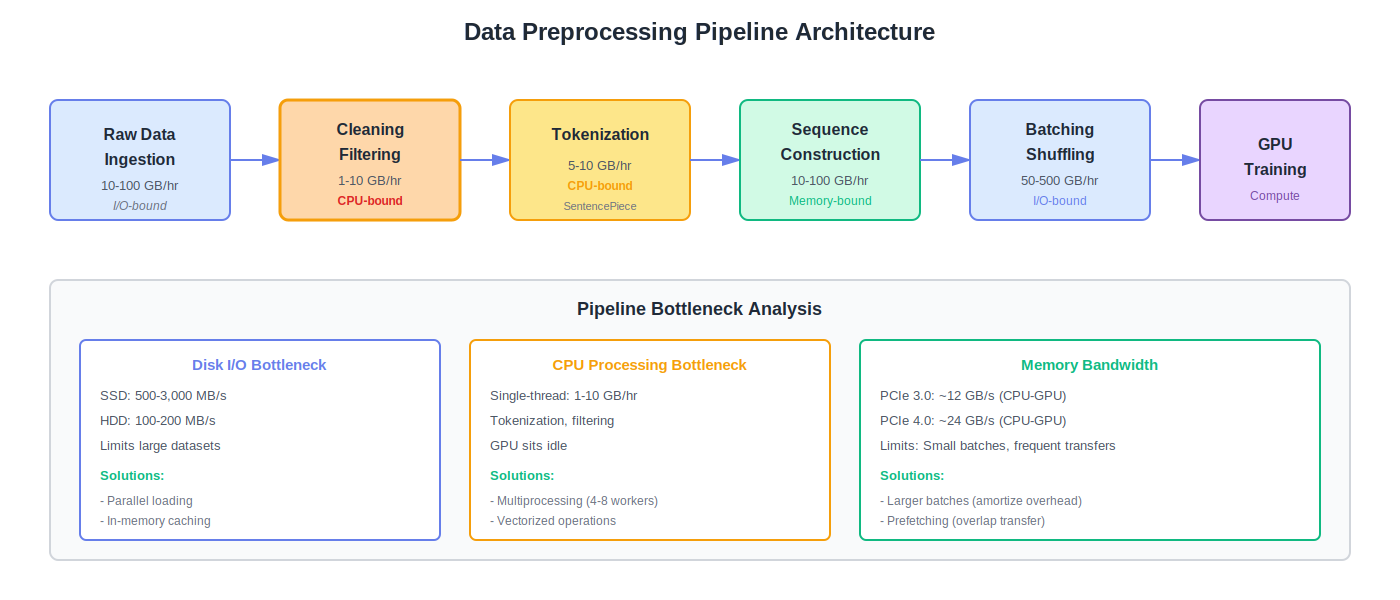
\includegraphics[width=0.95\textwidth]{chapters/diagrams/chapter08_data_pipeline_a1b2c3d4.pdf}
\caption{Data preprocessing pipeline architecture showing stages from raw data ingestion through batching. Bottlenecks typically occur at cleaning/filtering (CPU-bound) and disk I/O (storage-bound) stages.}
\label{fig:data_pipeline}
\end{figure}


\subsection{Pipeline Cost Analysis}

Pipeline infrastructure costs vary by scale and optimization level. Small-scale pipelines handling under 100 GB of data on a single machine require \$50-200 for SSD storage, with compute included in the training machine. Engineering effort of 1-2 weeks for setup dominates costs at \$10,000-20,000. This configuration suffices for initial development and small-scale experiments.

Medium-scale pipelines handling 100 GB to 10 TB of data across distributed systems require \$500-5,000 for distributed SSD or object storage. Compute needs expand to 4-16 preprocessing nodes. Engineering effort increases to 4-8 weeks for setup and optimization, totaling \$50,000-150,000. This scale supports regular training runs and moderate experimentation.

Large-scale pipelines exceeding 10 TB of data with production requirements demand \$5,000-50,000 for distributed object storage with redundancy. Dedicated preprocessing clusters handle continuous data flow. Engineering effort spans 3-6 months for development of robust, monitored pipelines, totaling \$200,000-1,000,000. This investment makes sense only for organizations running continuous training or large-scale experimentation programs.

The optimization decision hinges on training frequency and scale. For one-time training runs, simple pipelines suffice—the engineering cost of optimization exceeds the compute savings. For continuous training or large-scale experimentation, optimized pipelines provide substantial ROI. A pipeline that reduces training time by 30\% saves \$15,000 on a \$50,000 training run, justifying significant engineering investment after just a few runs.

\section{Data Augmentation and Synthetic Data}

\subsection{Augmentation Strategies}

Data augmentation artificially expands training datasets through transformations that preserve semantic meaning while introducing variation. This technique reduces data collection costs and improves model robustness by exposing the model to diverse phrasings and formulations of similar content.

Back-translation translates text to another language and back, introducing paraphrasing while preserving meaning. Using translation APIs costs \$0.001-0.01 per example, far less than human annotation. Effectiveness varies by task: low-resource tasks see 10-30\% accuracy improvement, while high-resource tasks see 5-10\% improvement. The technique works best for tasks where paraphrasing doesn't change labels, such as sentiment analysis or topic classification.

Synonym replacement substitutes words with synonyms from WordNet or embedding-based similarity. Computational cost is negligible—a few milliseconds per example. Effectiveness reaches 5-15\% improvement for classification tasks, though care must be taken to avoid changing meaning. The technique fails for tasks requiring precise wording, such as named entity recognition or question answering.

Random insertion, deletion, and swapping introduce noise that improves model robustness. These techniques cost nothing computationally and provide 3-8\% improvement on classification tasks. The approach works by forcing the model to focus on semantic content rather than specific word positions or exact phrasing. Effectiveness depends on noise level—too little provides minimal benefit, too much degrades training signal.

Contextual word replacement uses language models to generate contextually appropriate substitutions. This technique costs \$0.0001-0.001 per example using API-based language models, or runs locally at negligible cost with open-source models. Effectiveness reaches 10-20\% improvement for tasks requiring semantic understanding. The technique generates more natural variations than simple synonym replacement, though at higher computational cost.

\subsection{Synthetic Data Generation}

Synthetic data generation creates training examples programmatically, reducing or eliminating human annotation costs. This approach works best when the generation process can be validated and when synthetic examples closely match production distribution.

Template-based generation creates examples from predefined patterns. For structured tasks like form filling or database queries, templates can generate millions of valid examples at near-zero cost. A template for customer support queries might generate "I need help with [product] [issue]" with systematic variation of products and issues. This approach works when the task structure is well-defined and the template space covers production distribution adequately.

Rule-based generation applies domain rules to create valid examples. For code generation tasks, syntax rules ensure generated code is valid. For data extraction tasks, rules define valid entity relationships. The cost is primarily engineering time to develop and validate rules—typically 2-4 weeks for a comprehensive rule set. Once developed, generation costs are negligible. Effectiveness depends on rule coverage: comprehensive rules generate high-quality data, incomplete rules introduce systematic biases.

Model-based generation uses trained language models to generate examples. GPT-4 or similar models can generate training data at \$0.01-0.10 per example, still cheaper than human annotation at \$0.50-5.00 per example. Quality varies significantly: simple tasks yield 80-90\% usable examples, complex tasks yield 40-60\% usable examples. Human review remains necessary to filter low-quality generations, but the cost savings can reach 50-70\% compared to full human annotation.

The critical consideration for synthetic data is distribution match. Synthetic examples that differ systematically from production data degrade model performance despite high volume. Validation requires comparing synthetic and production distributions across multiple dimensions: vocabulary, syntax, semantic patterns, and edge cases. Mismatches indicate the need for generation process refinement or supplemental real data collection.

\subsection{Augmentation Economics}

Data augmentation economics follow a clear pattern: augmentation costs far less than original data collection, but provides diminishing returns. The first 2× data expansion through augmentation typically costs 5-10\% of original collection costs and provides 10-20\% accuracy improvement. The next 2× expansion costs similar amounts but provides only 5-10\% additional improvement. Beyond 4× expansion, returns diminish rapidly.

For a project with 10,000 labeled examples costing \$50,000 to collect, augmentation to 40,000 examples costs \$2,500-5,000 and might improve accuracy from 85\% to 92\%. Further augmentation to 160,000 examples costs another \$2,500-5,000 but might improve accuracy only to 94\%. The optimization question centers on whether the marginal accuracy improvement justifies the cost and whether collecting additional real data would provide better returns.

The strategic decision depends on data availability and task characteristics. When real data is scarce or expensive—medical imaging, specialized domains, rare events—aggressive augmentation makes sense. When real data is abundant and cheap—web text, common images, standard classification—minimal augmentation suffices, with resources better spent on data quality or model optimization.

\section{Training Monitoring and Evaluation}

\subsection{Monitoring Infrastructure}

Training monitoring tracks model convergence, identifies issues early, and enables informed intervention decisions. Effective monitoring prevents wasted compute from failed training runs and provides data for optimization decisions.

Loss curves track training and validation loss over time, providing the primary signal of training progress. Training loss should decrease steadily; plateaus indicate learning rate issues or optimization problems. Validation loss should track training loss initially, then diverge as the model begins overfitting. The gap between training and validation loss quantifies overfitting severity. Monitoring both curves enables early stopping—terminating training when validation loss stops improving—saving compute resources that would otherwise be wasted on overfitting.

Learning rate schedules require monitoring to ensure appropriate adjustment timing. Warmup periods at the start of training prevent instability from large initial updates. Decay schedules reduce learning rate as training progresses, enabling fine-grained optimization. Monitoring loss curves during schedule transitions identifies whether adjustments occur at appropriate times. Premature decay slows learning unnecessarily; delayed decay wastes compute on suboptimal updates.

Gradient statistics reveal optimization health. Gradient norms that grow unboundedly indicate instability requiring learning rate reduction or gradient clipping. Gradient norms that approach zero indicate vanishing gradients, suggesting architectural issues or learning rate problems. Monitoring gradient statistics enables early detection of training failures before they waste significant compute resources.

Resource utilization monitoring tracks GPU utilization, memory consumption, and data loading throughput. Low GPU utilization indicates data loading bottlenecks or inefficient batching. High memory consumption approaching limits suggests batch size reduction or gradient accumulation. Monitoring these metrics enables infrastructure optimization and prevents out-of-memory failures that waste training progress.

\begin{figure}[htbp]
\centering
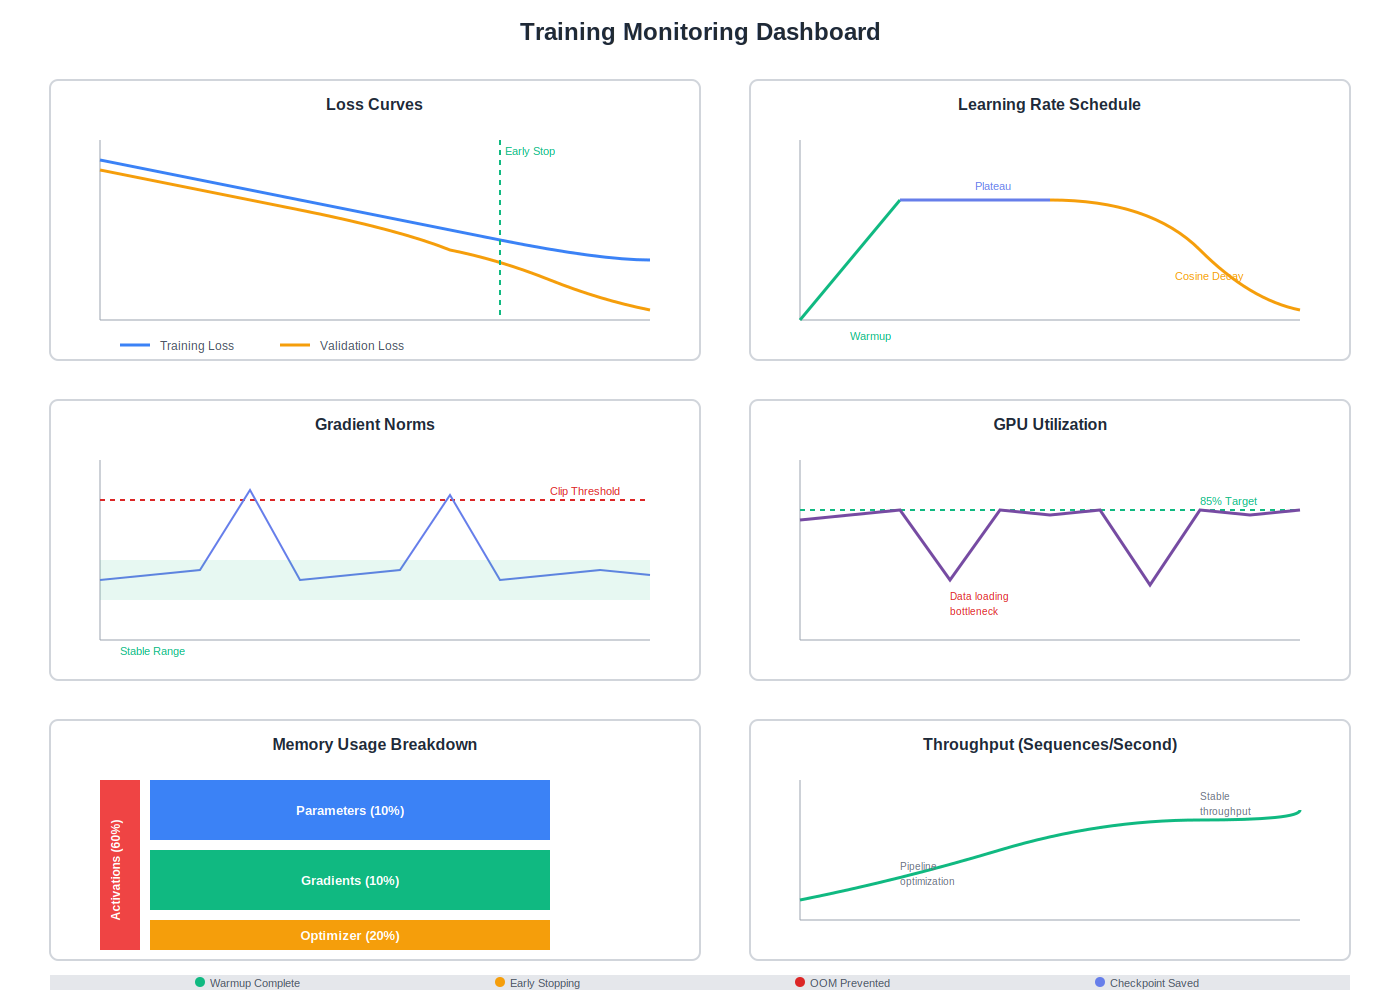
\includegraphics[width=0.95\textwidth]{chapters/diagrams/chapter08_monitoring_q7r8s9t0.pdf}
\caption{Training monitoring dashboard showing key metrics: loss curves with early stopping point, learning rate schedule phases, gradient norms with clipping threshold, GPU utilization with data loading spikes, memory breakdown by component, and throughput improvements over time. Comprehensive monitoring enables early issue detection and informed intervention decisions.}
\label{fig:monitoring_dashboard}
\end{figure}

\subsection{Evaluation Frameworks}

Evaluation frameworks measure model performance on held-out test data, providing unbiased estimates of production performance. The framework design determines whether evaluation results predict production success or mislead with optimistic estimates.

Test set construction requires careful attention to distribution match. Test data should represent production distribution across all relevant dimensions: input types, edge cases, and temporal variation. Systematic differences between test and production distributions lead to evaluation-production performance gaps that undermine deployment confidence. For time-series data, temporal splits prevent data leakage; for user-generated content, user-based splits prevent overfitting to specific users.

Metric selection should align with business objectives. Accuracy measures overall correctness but may hide performance issues on important subgroups. Precision and recall trade off false positives versus false negatives, with optimal balance depending on error costs. F1 score balances precision and recall but may not reflect business priorities. For imbalanced datasets, metrics like AUC-ROC or average precision provide more informative evaluation than raw accuracy.

Subgroup analysis identifies performance disparities across important segments. A model with 90\% overall accuracy might achieve 95\% on common cases but only 70\% on rare but important cases. Analyzing performance by input type, user segment, or edge case category reveals these disparities. Production deployment requires acceptable performance across all critical segments, not just high average performance.

Error analysis examines failure cases to identify systematic issues. Clustering errors by type—missing information, ambiguous inputs, edge cases—reveals whether failures are random or systematic. Systematic failures indicate training data gaps, architectural limitations, or preprocessing issues that can be addressed. Random failures may represent irreducible task difficulty. The distinction determines whether additional investment can improve performance or whether current performance represents a practical ceiling.

\begin{tcolorbox}[colback=red!5!white,colframe=red!75!black,title=\textbf{COMMON MISTAKES: Evaluation Pitfalls}]

\textbf{Data Leakage}: Test data that overlaps with training data produces optimistic performance estimates that don't generalize to production. This occurs through duplicate examples, temporal leakage in time-series data, or information leakage through preprocessing. Rigorous data splitting and validation prevents this issue.

\textbf{Metric Mismatch}: Optimizing for metrics that don't align with business objectives leads to models that perform well on benchmarks but poorly in production. A customer support model optimized for accuracy might achieve high scores by handling easy queries well while failing on difficult but important cases. Metric selection should reflect actual business priorities and error costs.

\textbf{Insufficient Test Coverage}: Test sets that don't represent production distribution lead to evaluation-production performance gaps. A model tested only on clean, well-formatted inputs may fail on noisy production data. Test sets should include edge cases, adversarial examples, and distribution shifts likely in production.

\end{tcolorbox}

\section{Hyperparameter Optimization}

\subsection{Optimization Strategies}

Hyperparameter optimization searches for configurations that maximize model performance. The search space includes learning rate, batch size, model architecture parameters, regularization strength, and optimizer settings. Effective optimization balances exploration of the search space against computational cost.

Grid search evaluates all combinations of predefined hyperparameter values. For three hyperparameters with five values each, this requires 125 training runs. The approach guarantees finding the best combination within the search space but becomes prohibitively expensive for large search spaces. Grid search works best for small search spaces with 2-3 hyperparameters and 3-5 values each, requiring 10-100 training runs.

Random search samples hyperparameter combinations randomly from defined ranges. This approach explores the search space more efficiently than grid search, often finding good configurations with fewer evaluations. For the same computational budget as grid search, random search typically finds better configurations by exploring more diverse combinations. The approach works well for medium search spaces with 4-6 hyperparameters, requiring 50-200 training runs to find near-optimal configurations.

Bayesian optimization builds a probabilistic model of the hyperparameter-performance relationship and uses this model to guide search toward promising regions. This approach requires fewer evaluations than random search—typically 20-50 training runs—but adds optimization overhead. The technique works best for expensive training runs where minimizing evaluations justifies the optimization complexity. Tools like Optuna and Ray Tune provide production-ready Bayesian optimization implementations.

Population-based training runs multiple training processes in parallel, periodically copying hyperparameters from high-performing runs to low-performing runs. This approach combines hyperparameter search with training, reducing total wall-clock time. The technique requires substantial parallel compute resources—typically 10-50 simultaneous training runs—but can find good configurations faster than sequential approaches. The method works best when parallel compute is available and training time is the primary constraint.

\begin{figure}[htbp]
\centering
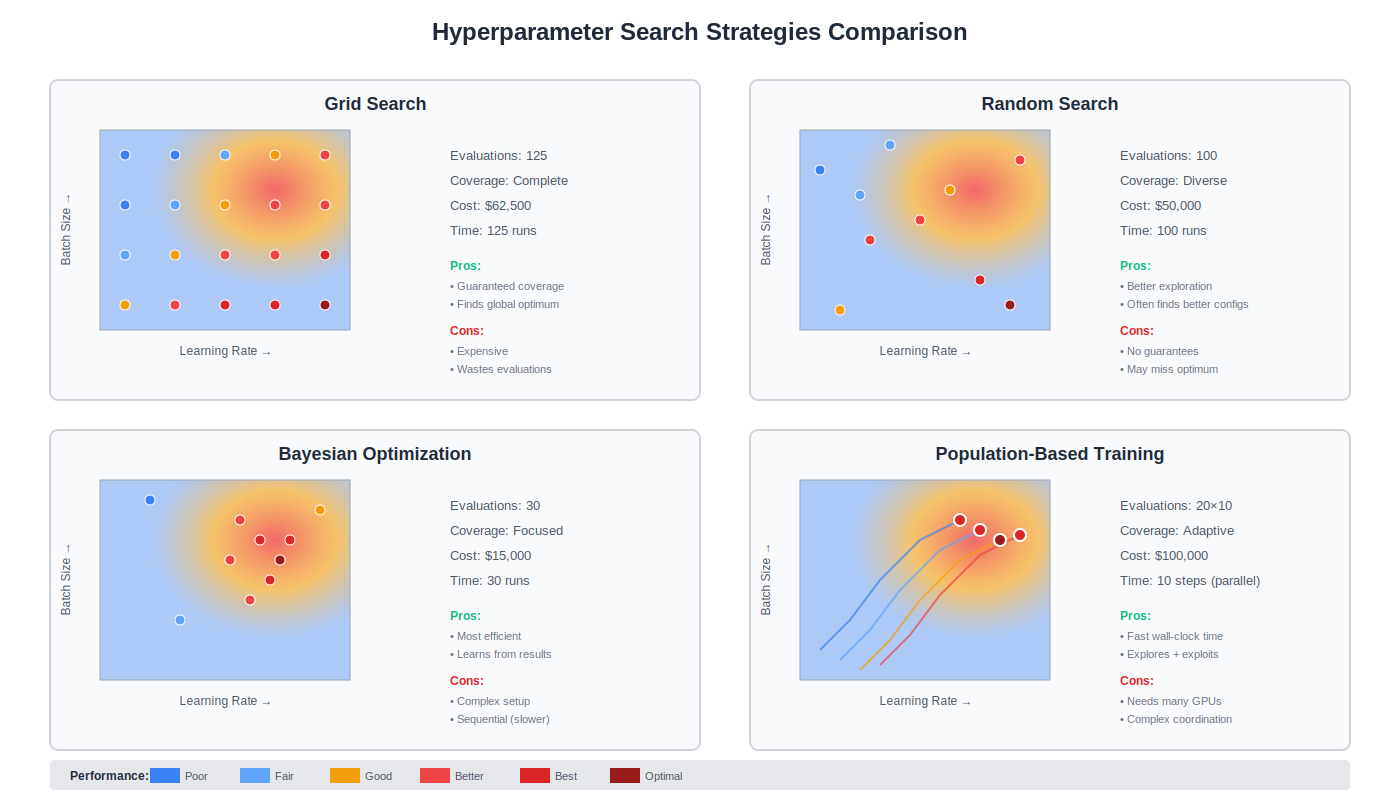
\includegraphics[width=0.95\textwidth]{chapters/diagrams/chapter08_hyperparameter_m3n4o5p6.pdf}
\caption{Hyperparameter search strategy comparison showing exploration patterns and efficiency trade-offs. Grid search provides complete coverage but wastes evaluations; random search explores more efficiently; Bayesian optimization focuses on promising regions; population-based training parallelizes search for faster wall-clock time.}
\label{fig:hyperparameter_search}
\end{figure}

\subsection{Optimization Economics}

Hyperparameter optimization costs scale with search space size and training cost per configuration. For BERT-base training costing \$500 per run, a 100-configuration random search costs \$50,000. This investment makes sense when the resulting model will be deployed at scale, where performance improvements translate to substantial operational savings or revenue increases.

The optimization strategy should match project economics. For research projects or one-time deployments, minimal optimization with 5-10 manual trials suffices. For production systems serving millions of requests, comprehensive optimization with 50-200 trials justifies its cost through improved performance. For continuous training pipelines, automated optimization infrastructure amortizes its development cost across multiple projects.

Early stopping and performance prediction reduce optimization costs by terminating unpromising configurations early. A configuration showing poor performance after 10\% of training is unlikely to become competitive by completion. Terminating such runs early saves 90\% of their compute cost. Across a 100-configuration search, early stopping might reduce total cost by 40-60\% by eliminating poor configurations quickly.

\section{Data Versioning and Reproducibility}

\subsection{Versioning Infrastructure}

Data versioning tracks dataset changes over time, enabling reproducibility and debugging. As training data evolves through collection, cleaning, and augmentation, versioning provides an audit trail of what data produced which model performance.

Dataset versioning systems like DVC (Data Version Control) or Pachyderm track dataset changes using content-addressable storage. Each dataset version receives a unique identifier based on its content. Models trained on specific dataset versions can be traced back to exact training data, enabling reproducibility and debugging. The storage cost depends on dataset size and change frequency: for 100 GB datasets with monthly updates, storage costs run \$50-200 monthly for cloud object storage with versioning.

Preprocessing pipeline versioning tracks code changes that transform raw data into training data. A bug in preprocessing can corrupt training data, degrading model performance in ways difficult to diagnose without versioning. Git-based versioning of preprocessing code combined with dataset versioning provides complete reproducibility. The engineering cost is minimal—standard version control practices—but the debugging value is substantial when issues arise.

Experiment tracking systems like Weights & Biases, MLflow, or Neptune link models to dataset versions, hyperparameters, and training code. This linkage enables reproducing any training run exactly and understanding what changed between runs. For teams running dozens or hundreds of experiments, this tracking infrastructure is essential for maintaining productivity and avoiding duplicate work.

\subsection{Reproducibility Practices}

Reproducibility requires controlling all sources of randomness and variation. Random seeds for data shuffling, weight initialization, and dropout must be fixed and recorded. Hardware differences—GPU models, driver versions, library versions—can affect results, requiring documentation. The goal is not perfect bit-level reproducibility, which is often impractical, but rather the ability to reproduce results within acceptable tolerance.

Containerization using Docker or similar tools captures the complete software environment, including library versions, system dependencies, and configuration. A containerized training environment can be archived and rerun months or years later, producing comparable results. The storage cost is minimal—typically a few GB per container—while the reproducibility value is substantial for debugging and auditing.

Documentation practices complement technical versioning. Training run documentation should include dataset version, preprocessing pipeline version, hyperparameters, training duration, final performance metrics, and any anomalies observed. This documentation enables future debugging and provides context for comparing runs. The time cost is 10-15 minutes per training run, negligible compared to training time but valuable for long-term project management.

\section{Key Insights}

\textbf{Data Quality Dominates Architecture}: Model performance depends more on training data quality than architectural sophistication. A well-designed model trained on poor data underperforms a simpler model trained on high-quality data. Data quality investment—annotation accuracy, coverage, consistency—provides better returns than architectural complexity for most applications.

\textbf{Pipeline Bottlenecks Waste Compute}: Data loading bottlenecks cause GPU idle time, wasting expensive compute resources. A GPU capable of 1,000 sequences per second achieves only 100 sequences per second if data loading provides only 100 sequences per second. Pipeline optimization—parallel loading, prefetching, caching—directly improves training efficiency and reduces costs.

\textbf{Augmentation Shows Diminishing Returns}: The first 2× data expansion through augmentation provides 10-20\% accuracy improvement at 5-10\% of original collection cost. Further expansion provides diminishing returns. Beyond 4× expansion, collecting additional real data typically provides better returns than additional augmentation.

\textbf{Monitoring Prevents Wasted Compute}: Early detection of training failures through monitoring prevents wasted compute on failed runs. Loss curves, gradient statistics, and resource utilization monitoring enable intervention before significant resources are consumed. For expensive training runs, monitoring infrastructure pays for itself by preventing a single failed run.

\textbf{Hyperparameter Optimization Costs Scale Rapidly}: Comprehensive hyperparameter search with 100+ configurations can cost 100× a single training run. This investment makes sense for production deployments at scale but not for research projects or one-time applications. Optimization strategy should match deployment scale and expected operational lifetime.

\textbf{Versioning Enables Debugging}: Data and code versioning provide an audit trail that enables reproducing results and debugging performance issues. When model performance degrades, versioning enables identifying what changed—data, preprocessing, hyperparameters, or code. The infrastructure cost is minimal compared to the debugging value when issues arise.

The next chapter examines team building and organizational structure for AI projects, focusing on role definitions, skill requirements, and collaboration patterns that enable effective execution.



% Chapter 9: Operationalization (8 pages)
\chapter{Operationalization}

\section*{Why This Matters}

Production deployment represents only the beginning of a model's operational lifecycle. Models require ongoing management, monitoring, and maintenance to sustain performance and deliver business value. Unlike traditional software, which remains stable once deployed, machine learning models degrade over time as production data distributions shift, requiring systematic retraining, version management, and continuous evaluation.

The operational phase typically accounts for 60-80\% of total AI system costs over a three-year horizon. Training a model might cost \$50,000, but operating it—serving predictions, monitoring performance, retraining periodically, managing versions, and maintaining infrastructure—costs \$150,000-\$400,000 annually. Understanding these operational requirements is essential for realistic budget planning, infrastructure sizing, and organizational capability assessment.

This chapter examines the technical and economic factors governing production AI operations, covering model lifecycle management, continuous training strategies, security considerations, and cost optimization approaches. The focus is on building sustainable operational practices that maintain model performance while controlling costs.

\section{Model Lifecycle Management}

Production models progress through distinct lifecycle stages, each with specific technical requirements and operational characteristics. Managing this lifecycle effectively requires version control systems, deployment strategies, and rollback capabilities comparable to traditional software engineering, but adapted for the unique characteristics of machine learning systems.

\subsection{Lifecycle Stages}

Models transition through research, staging, and production environments, with each stage serving specific validation purposes. The research environment supports experimentation and initial development, typically using smaller datasets and less expensive hardware. Models in research undergo rapid iteration, with dozens or hundreds of training runs exploring architectural variations, hyperparameter settings, and data preprocessing approaches. Infrastructure costs remain modest—perhaps \$5,000-\$20,000 monthly for a team of 5-10 researchers using shared GPU clusters.

The staging environment replicates production conditions for final validation before deployment. Staging uses production-scale data, production-equivalent hardware, and production API interfaces. This environment validates performance under realistic conditions, tests integration with downstream systems, and measures actual latency and throughput. Staging infrastructure typically mirrors production at 10-20\% scale, sufficient for load testing and integration validation without full production costs. For a production system serving 1,000 requests per second, staging might handle 100-200 requests per second, costing \$10,000-\$30,000 monthly.

Production represents the operational environment serving live traffic. Production infrastructure must provide the reliability, performance, and scalability required for business operations. This includes redundancy for high availability, monitoring for performance tracking, and capacity for peak load handling. Production costs scale with traffic volume and latency requirements. A system serving 1,000 requests per second with 100ms latency requirements might cost \$50,000-\$150,000 monthly, depending on model size and optimization level.

\subsection{Version Management}

Model versioning requires tracking not just model weights, but the complete artifact set necessary for reproducible deployment: training code, data preprocessing pipelines, hyperparameter configurations, dependency versions, and evaluation metrics. Unlike code versioning, which tracks text files, model versioning handles multi-gigabyte binary artifacts and complex dependency graphs.

A comprehensive version management system tracks model artifacts with unique identifiers linking to specific training runs. For a BERT-base model, this includes the 440 MB model checkpoint, the tokenizer vocabulary and configuration, the preprocessing pipeline code, the training dataset version or hash, the hyperparameter configuration, and the evaluation metrics on validation and test sets. Storage costs accumulate quickly: maintaining 50 model versions at 500 MB each consumes 25 GB, costing approximately \$0.60 monthly on S3 standard storage, but potentially \$25-\$50 monthly when including associated metadata, logs, and evaluation artifacts.

Version metadata enables critical operational capabilities. Each version records training date, training duration and cost, dataset version, evaluation metrics across multiple test sets, deployment history, and performance monitoring data. This metadata supports impact analysis when issues arise, cost attribution for budget tracking, and compliance documentation for regulated industries.

\subsection{Deployment Patterns}

Production deployment strategies balance risk mitigation against operational complexity. Three primary patterns—blue-green deployment, canary deployment, and shadow deployment—offer different trade-offs between safety, resource requirements, and validation thoroughness.

Blue-green deployment maintains two complete production environments, switching traffic between them atomically. The blue environment serves production traffic while the green environment receives the new model version. After validation in the green environment, traffic switches completely from blue to green. This approach provides instant rollback capability—simply switch traffic back to blue if issues arise—and zero-downtime deployment. However, it requires double the infrastructure capacity during deployment windows, increasing costs by 50-100\% during these periods. For a system normally costing \$100,000 monthly, blue-green deployment adds \$50,000-\$100,000 in temporary infrastructure costs per deployment.

Canary deployment gradually shifts traffic to the new model version, starting with a small percentage and increasing as confidence grows. Initial deployment might route 1\% of traffic to the new version, increasing to 5\%, 10\%, 25\%, 50\%, and finally 100\% over hours or days. This approach limits blast radius—if the new version performs poorly, only a small fraction of users are affected—and provides real-world validation before full deployment. Canary deployment requires sophisticated traffic routing and monitoring infrastructure, but adds minimal infrastructure costs beyond the new model version's serving capacity.

Shadow deployment runs the new model version in parallel with the current production version, logging predictions without serving them to users. This approach enables thorough validation with zero user impact, comparing new and old model predictions on real production traffic. Shadow deployment requires additional serving capacity equal to the new model's requirements—effectively doubling inference costs during the shadow period—but provides the highest confidence validation. For critical systems where deployment failures carry significant business risk, the additional cost of shadow deployment often justifies the risk reduction.

\subsection{Rollback Strategies}

Effective rollback capabilities require maintaining previous model versions in deployable state and implementing automated rollback triggers. The previous production version should remain deployed and ready to receive traffic, enabling rollback within seconds or minutes rather than hours. This requires keeping the previous version's serving infrastructure active, adding 10-20\% to infrastructure costs but providing essential risk mitigation.

Automated rollback triggers monitor key performance indicators and revert to the previous version when degradation exceeds thresholds. Typical triggers include error rate increases beyond baseline, latency degradation beyond SLA requirements, prediction distribution shifts indicating model failure, and business metric degradation such as conversion rate drops. For a model normally maintaining 0.1\% error rate and 50ms p95 latency, rollback might trigger automatically if error rate exceeds 0.5\% or latency exceeds 100ms for more than 5 minutes.

\begin{figure}[htbp]
\centering
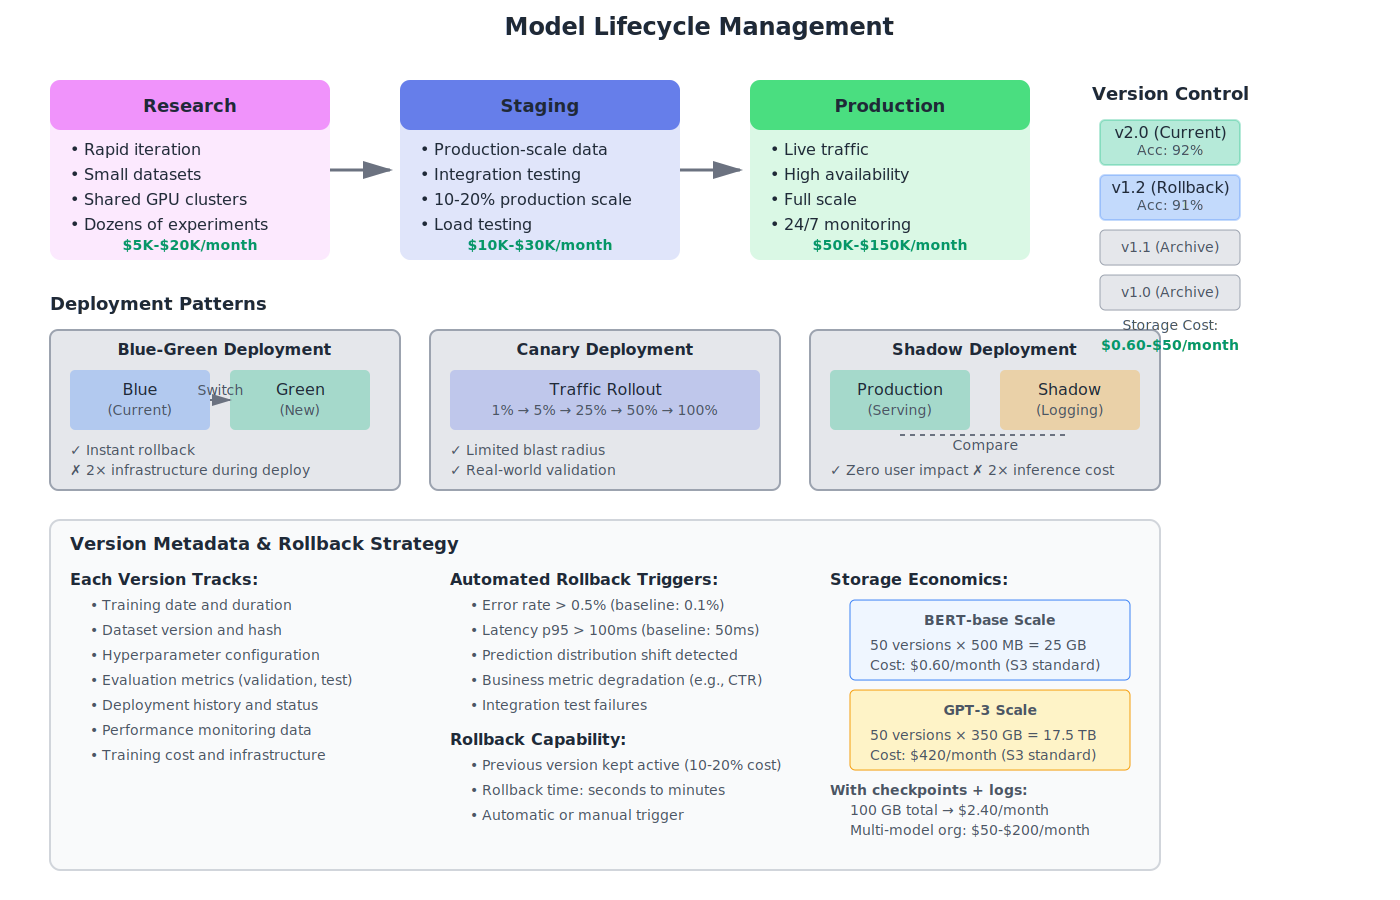
\includegraphics[width=0.95\textwidth]{chapters/diagrams/chapter09_lifecycle_q1r2s3t4.png}
\caption{Model lifecycle management showing progression from research through production environments, deployment patterns (blue-green, canary, shadow), version control strategy, and storage economics. Each environment stage has distinct characteristics and cost profiles, with production requiring the highest reliability and scale.}
\label{fig:lifecycle}
\end{figure}

\subsection{Storage Costs}

Model artifact storage costs scale with version retention policies and artifact sizes. A retention policy maintaining the current production version, the previous production version for rollback, the last 10 staging versions for analysis, and monthly snapshots for the past year generates specific storage requirements. For BERT-base models at 500 MB per version, this policy requires approximately 6 GB storage, costing \$0.15 monthly on S3 standard storage. For GPT-3 scale models at 350 GB per version, the same policy requires 4.2 TB, costing \$100 monthly.

Storage costs increase significantly when including training checkpoints, evaluation datasets, and experiment logs. A comprehensive artifact repository for a production model might include 50 model versions at 500 MB each (25 GB), 100 training checkpoints at 500 MB each (50 GB), evaluation datasets and results (10 GB), and training logs and metrics (15 GB), totaling 100 GB and costing \$2.40 monthly on S3 standard storage. For organizations managing dozens of production models, storage costs reach \$50-\$200 monthly, modest compared to training and serving costs but requiring management to prevent unbounded growth.

\section{Continuous Training and Evaluation}

Model performance degrades over time as production data distributions shift from training data distributions. This degradation, called model drift or concept drift, necessitates periodic retraining to maintain performance. Understanding when to retrain, how to automate the retraining process, and how to evaluate ongoing performance is essential for sustainable production operations.

\subsection{Model Drift and Retraining Triggers}

Model drift manifests as gradual performance degradation on production data. A sentiment analysis model trained on 2023 data might achieve 92\% accuracy initially, but degrade to 88\% accuracy after six months as language patterns evolve, new products and brands emerge, and cultural references shift. The degradation rate varies by domain: news and social media models drift rapidly (weeks to months), e-commerce and search models drift moderately (months to quarters), and medical and legal models drift slowly (quarters to years).

Retraining triggers should be based on measured performance degradation rather than fixed schedules. Continuous evaluation on held-out test sets or human-labeled production samples provides ongoing performance measurement. When performance drops below acceptable thresholds—for example, accuracy falling from 92\% to 89\%, or precision dropping from 85\% to 80\%—retraining becomes necessary. This approach ensures retraining occurs when needed rather than on arbitrary schedules, optimizing the trade-off between performance maintenance and retraining costs.

Data distribution shifts provide an earlier signal than performance degradation. Monitoring input feature distributions, prediction distributions, and confidence scores can detect drift before performance degrades significantly. For a model trained on data with mean feature values of 0.5 and standard deviation 0.2, production data showing mean 0.6 and standard deviation 0.3 indicates distribution shift likely to cause performance degradation. Triggering retraining based on distribution shift enables proactive maintenance before user-visible performance issues arise.

\subsection{Retraining Costs and Economics}

Retraining costs depend on model size, dataset size, and retraining frequency. For BERT-base trained on 10 million documents, retraining from scratch requires approximately 20 GPU-hours on A100 hardware, costing \$50-\$100 on cloud spot instances. Retraining quarterly costs \$200-\$400 annually. For larger models, costs scale proportionally: a GPT-3 scale model requiring 1,000 GPU-days for initial training might require 100-200 GPU-days for retraining on updated data, costing \$250,000-\$500,000 per retraining cycle.

Fine-tuning from the previous model version rather than training from scratch reduces costs significantly. Fine-tuning typically requires 10-20\% of full training time, as the model already captures general patterns and needs only to adapt to distribution shifts. For BERT-base, fine-tuning might require 2-4 GPU-hours, costing \$5-\$10. This 10× cost reduction makes more frequent retraining economically viable, enabling monthly or even weekly updates for rapidly drifting domains.

The economic trade-off balances retraining costs against performance degradation costs. If model accuracy degradation from 92\% to 89\% costs \$10,000 monthly in lost revenue or increased support costs, spending \$1,000 monthly on retraining provides strong ROI. Conversely, if performance degradation has minimal business impact, less frequent retraining makes economic sense. This calculation should drive retraining frequency decisions rather than arbitrary schedules.

\subsection{Continuous Evaluation Strategy}

Continuous evaluation requires ongoing measurement of model performance on production data. Three primary approaches—held-out test sets, human labeling of production samples, and proxy metrics—provide different trade-offs between cost, accuracy, and timeliness.

Held-out test sets provide consistent performance measurement over time. Maintaining a fixed test set of 10,000 labeled examples enables tracking performance trends as the model and production data evolve. However, held-out test sets become stale, eventually diverging from production data distribution and providing misleading performance estimates. Test set maintenance requires periodic updates with recent production data, necessitating human labeling costs.

Human labeling of production samples provides accurate performance measurement on current data. Randomly sampling 100-1,000 production examples weekly or monthly and obtaining human labels enables direct performance measurement. For a model serving 1 million predictions monthly, sampling 1,000 examples (0.1\%) and obtaining labels at \$0.50 per example costs \$500 monthly. This approach provides accurate, current performance measurement but requires ongoing labeling budget.

Proxy metrics provide real-time performance signals without human labeling. For a recommendation system, click-through rate serves as a proxy for recommendation quality. For a search system, query reformulation rate indicates search quality. For a content moderation system, user report rate signals moderation accuracy. Proxy metrics enable continuous monitoring at zero marginal cost, but require validation against ground truth labels to ensure correlation with actual performance.

\begin{figure}[htbp]
\centering
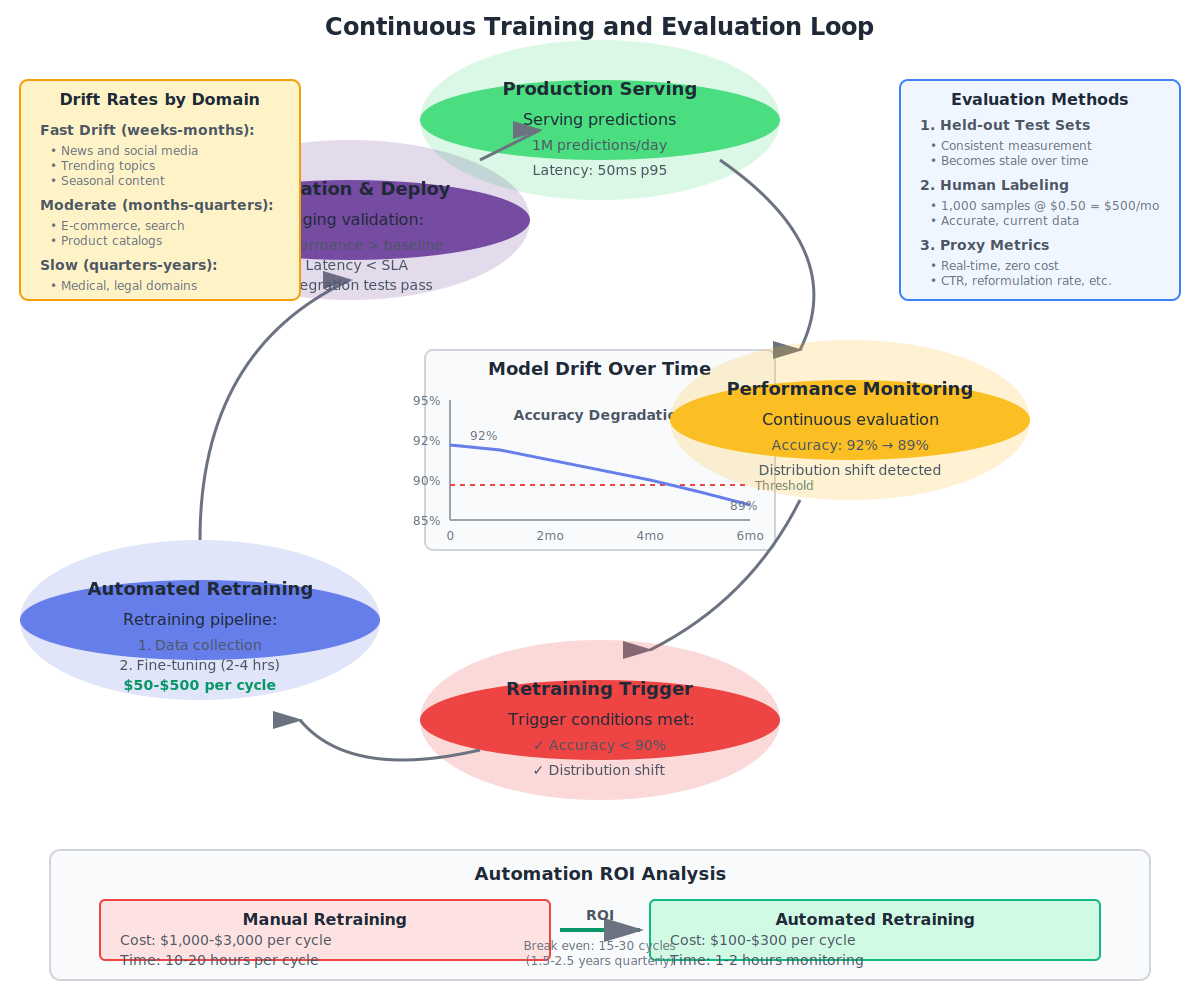
\includegraphics[width=0.95\textwidth]{chapters/diagrams/chapter09_continuous_training_u5v6w7x8.png}
\caption{Continuous training and evaluation loop showing the complete cycle from production serving through performance monitoring, drift detection, automated retraining, and validation. The center graph illustrates model drift over time, with performance degrading from 92\% to 89\% over six months, triggering retraining when the 90\% threshold is crossed.}
\label{fig:continuous_training}
\end{figure}

\subsection{Automation ROI}

Automating the retraining pipeline—data collection, preprocessing, training, evaluation, and deployment—requires upfront engineering investment but provides ongoing operational cost savings. Building a fully automated retraining pipeline typically requires 2-4 engineer-months of effort, costing \$40,000-\$100,000 in engineering time. This investment pays off when retraining frequency and manual effort justify automation.

Manual retraining requires data scientist time for each cycle: collecting and preprocessing data (4-8 hours), configuring and launching training (2-4 hours), evaluating results (2-4 hours), and coordinating deployment (2-4 hours), totaling 10-20 hours per retraining cycle. At \$100-\$150 per hour for data scientist time, manual retraining costs \$1,000-\$3,000 per cycle. Retraining quarterly costs \$4,000-\$12,000 annually; retraining monthly costs \$12,000-\$36,000 annually.

Automated retraining reduces per-cycle costs to infrastructure and monitoring time. After initial automation investment, each retraining cycle requires only monitoring and validation time (1-2 hours), costing \$100-\$300 per cycle. The automation investment breaks even after 15-30 retraining cycles, or 1.5-2.5 years for quarterly retraining, 1-2 years for monthly retraining. For models requiring frequent retraining or organizations managing multiple production models, automation provides clear ROI.

\section{Security and Privacy}

Production AI systems face security threats and privacy requirements distinct from traditional software systems. Model theft, adversarial attacks, data poisoning, and privacy violations represent real risks with significant business and legal consequences. Understanding these threats and implementing appropriate defenses is essential for responsible production deployment.

\subsection{Attack Surface and Threats}

AI systems present multiple attack surfaces. Model theft through API access represents a significant threat: attackers can query a production model repeatedly, collect input-output pairs, and train a substitute model that replicates the original's behavior. For a model serving 1,000 requests per second, an attacker making 10 queries per second for 24 hours collects 864,000 input-output pairs, potentially sufficient to train a substitute model. Rate limiting, query monitoring, and watermarking provide partial defenses, but determined attackers with sufficient resources can often extract substantial model functionality.

Adversarial attacks craft inputs designed to cause model failures. For image classifiers, adversarial examples—images with imperceptible perturbations—can cause misclassification with high confidence. For text models, adversarial prompts can elicit inappropriate responses or leak training data. For recommendation systems, adversarial user behavior can manipulate recommendations. Defending against adversarial attacks requires adversarial training, input validation, and output filtering, adding 10-30\% to training costs and 5-15\% to inference latency.

Data poisoning attacks inject malicious examples into training data, causing models to learn attacker-desired behaviors. For models trained on user-generated content, attackers can create accounts and submit poisoned examples. For models trained on web-scraped data, attackers can publish poisoned content. Defending against data poisoning requires data validation, anomaly detection, and robust training procedures, adding 20-50\% to data preprocessing costs.

Privacy violations occur when models leak training data or enable inference about training examples. Models can memorize specific training examples, particularly rare or unusual ones, and reproduce them in responses. For models trained on sensitive data—medical records, financial information, personal communications—this leakage violates privacy regulations and creates legal liability. Differential privacy and federated learning provide technical defenses, but impose accuracy costs and implementation complexity.

\subsection{Security Techniques}

Rate limiting restricts the number of queries per user or API key, mitigating model theft and denial-of-service attacks. Typical rate limits range from 10-1,000 queries per minute depending on use case and user tier. Implementing rate limiting requires API gateway infrastructure and user authentication, adding \$500-\$2,000 monthly in infrastructure costs for systems serving millions of requests daily.

Query monitoring detects suspicious access patterns indicating potential attacks. Monitoring systems track query frequency, query similarity, error rates, and response patterns. Anomalous patterns—such as a single user making thousands of similar queries, or queries systematically exploring input space—trigger alerts or automatic blocking. Implementing comprehensive monitoring requires logging infrastructure, analysis pipelines, and alerting systems, costing \$2,000-\$10,000 monthly depending on query volume and analysis sophistication.

Model watermarking embeds detectable signatures in model outputs, enabling detection of stolen models. Watermarking techniques modify model behavior on specific trigger inputs, causing watermarked models to produce distinctive outputs. If a competitor's model produces the same distinctive outputs, this provides evidence of model theft. Watermarking adds minimal inference cost but requires careful implementation to avoid degrading model performance on normal inputs.

Adversarial training incorporates adversarial examples into training data, improving model robustness. Training on both normal and adversarial examples teaches models to handle perturbations and edge cases. Adversarial training typically increases training time by 20-50\% and training data requirements by 10-30\%, but significantly improves robustness. For BERT-base, adversarial training might increase training cost from \$1,000 to \$1,200-\$1,500.

\subsection{Privacy Techniques}

Differential privacy provides mathematical guarantees that model training does not leak information about individual training examples. Differential privacy adds calibrated noise during training, ensuring that model parameters do not depend too strongly on any single training example. This prevents memorization of sensitive data and provides formal privacy guarantees. However, differential privacy imposes accuracy costs: typical implementations reduce accuracy by 1-5 percentage points. For a model achieving 92\% accuracy without differential privacy, differentially private training might achieve 87-91\% accuracy.

Implementing differential privacy requires specialized training procedures and careful privacy budget management. Privacy budget—measured in epsilon—quantifies the privacy guarantee: smaller epsilon provides stronger privacy but larger accuracy costs. Typical values range from epsilon=1 (strong privacy, significant accuracy cost) to epsilon=10 (weaker privacy, minimal accuracy cost). Training with differential privacy increases training time by 20-40\% due to additional noise injection and gradient clipping operations.

Federated learning trains models on distributed data without centralizing the data. Instead of collecting data from edge devices or partner organizations, federated learning sends model updates to the data, trains locally, and aggregates only model parameter updates. This approach enables training on sensitive data that cannot be centralized due to privacy regulations or competitive concerns. Federated learning requires coordination infrastructure, secure aggregation protocols, and handling of heterogeneous data distributions, increasing training complexity and cost by 2-5×.

\begin{figure}[htbp]
\centering
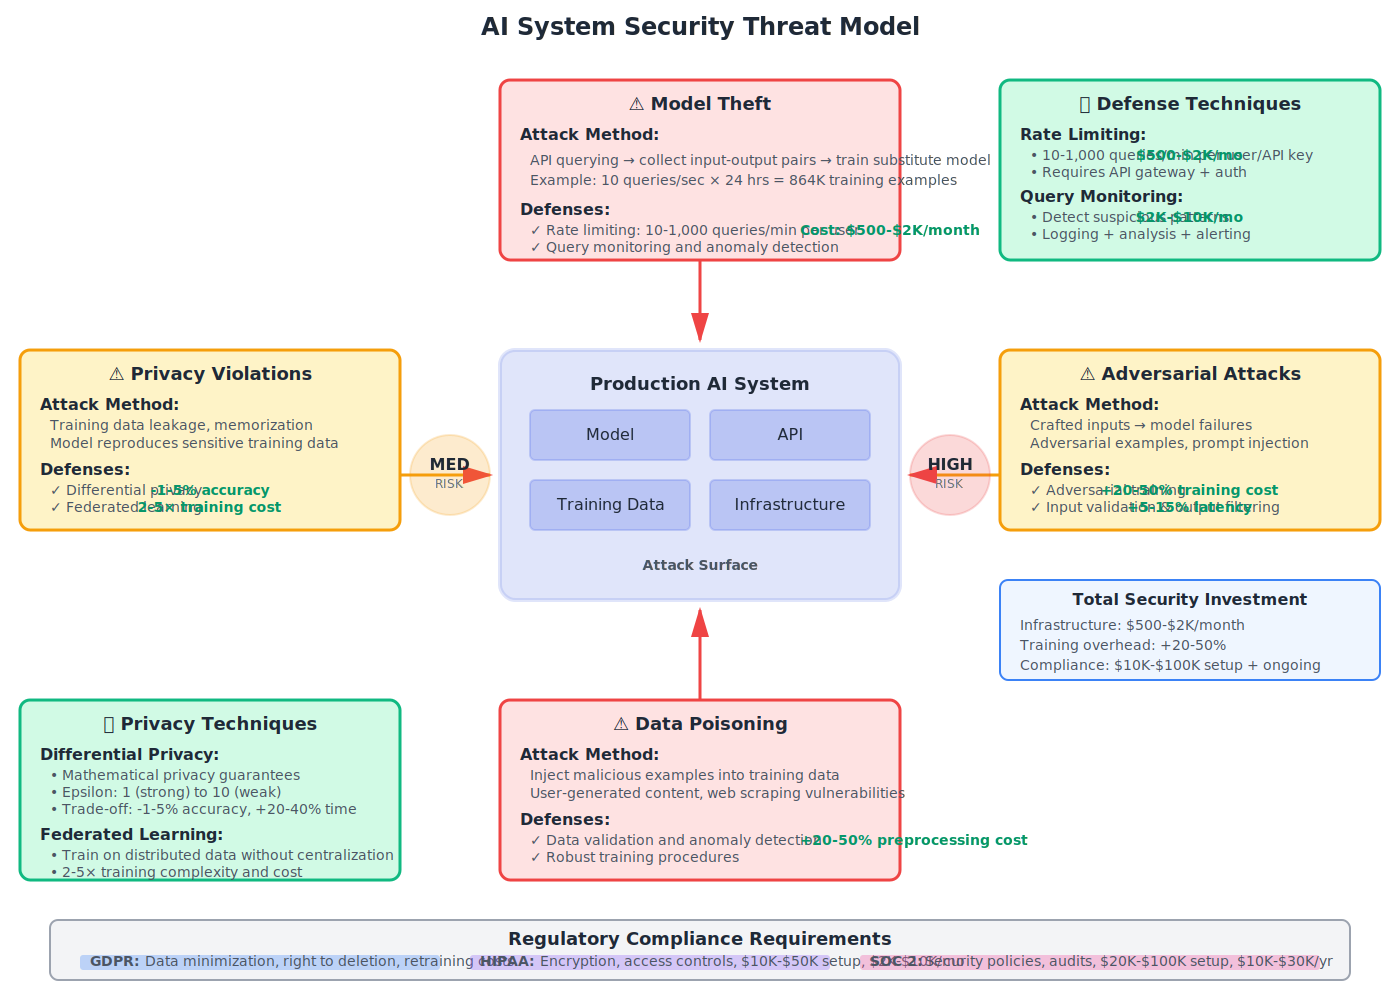
\includegraphics[width=0.95\textwidth]{chapters/diagrams/chapter09_security_threats_y9z0a1b2.png}
\caption{AI system security threat model showing four primary attack vectors: model theft through API querying, adversarial attacks with crafted inputs, data poisoning during training, and privacy violations through data leakage. Each threat includes attack methods, impacts, defense mechanisms, and associated costs. Regulatory compliance requirements (GDPR, HIPAA, SOC 2) are shown at the bottom.}
\label{fig:security_threats}
\end{figure}

\subsection{Compliance Requirements}

Regulatory compliance—GDPR in Europe, HIPAA for healthcare, SOC 2 for enterprise software—imposes specific technical and operational requirements. GDPR requires data minimization, purpose limitation, and the right to deletion. For AI systems, this means training only on necessary data, documenting data usage, and implementing mechanisms to remove individual data points from trained models. Model retraining after data deletion requests can cost \$1,000-\$100,000 depending on model size and retraining frequency.

HIPAA compliance for healthcare AI requires encryption of data at rest and in transit, access controls and audit logging, business associate agreements with vendors, and regular security assessments. Implementing HIPAA-compliant infrastructure typically costs \$10,000-\$50,000 in initial setup and \$2,000-\$10,000 monthly in ongoing compliance costs. These costs include encrypted storage, secure API gateways, audit logging infrastructure, and compliance monitoring.

SOC 2 compliance for enterprise software requires documented security policies, access controls, change management procedures, incident response plans, and annual audits. Achieving SOC 2 certification typically costs \$20,000-\$100,000 in initial implementation and \$10,000-\$30,000 annually for ongoing audits and compliance maintenance. For AI systems, SOC 2 compliance extends to model training, deployment, and monitoring processes.

\section{Cost Optimization Strategies}

Production AI costs typically break down as 40\% training, 50\% inference, and 10\% storage and operations. Understanding this breakdown and implementing targeted optimization strategies can reduce total costs by 30-70\% while maintaining performance and reliability.

\subsection{Training Cost Optimization}

Spot instances reduce training costs by 60-80\% compared to on-demand instances, but introduce interruption risk. Cloud providers offer unused capacity at steep discounts: AWS spot instances for p3.8xlarge (4× V100 GPUs) cost \$3.06 per hour versus \$12.24 on-demand. For training jobs requiring 100 GPU-hours, spot instances cost \$306 versus \$1,224 on-demand, saving \$918 (75\%). However, spot instances can be interrupted with 2-minute warning when capacity is needed elsewhere.

Handling spot interruptions requires checkpointing and automatic restart capabilities. Training code should save checkpoints every 10-30 minutes, enabling restart from the most recent checkpoint after interruption. Implementing robust checkpointing adds 5-10\% training time overhead but enables spot instance usage. For training jobs longer than 4-8 hours, spot instance savings exceed checkpointing overhead, providing net cost reduction.

Mixed precision training reduces training time and memory usage by 40-60\% with minimal accuracy impact. Training in FP16 instead of FP32 halves memory requirements and doubles throughput on modern GPUs with tensor cores. For BERT-base, mixed precision training reduces training time from 20 GPU-hours to 12 GPU-hours, saving \$20-\$40 per training run. Implementing mixed precision requires framework support (PyTorch AMP, TensorFlow mixed precision) and careful loss scaling to prevent numerical instability.

Gradient accumulation enables training with larger effective batch sizes on limited hardware. Instead of processing a 512-example batch in one step, gradient accumulation processes 8 batches of 64 examples, accumulating gradients before updating parameters. This technique enables training large models on smaller GPUs, avoiding the need for expensive multi-GPU setups. For models requiring 32 GB memory with batch size 512, gradient accumulation enables training on 16 GB GPUs, reducing hardware costs from \$2.50 per hour (A100 40GB) to \$1.20 per hour (A10G 24GB).

\subsection{Inference Cost Optimization}

Model compression reduces inference costs by 50-90\% through quantization, pruning, and distillation. Quantization converts FP32 weights to INT8, reducing model size by 75\% and increasing throughput by 2-4×. For BERT-base, quantization reduces model size from 440 MB to 110 MB and increases throughput from 100 to 300 sequences per second on CPU. This enables serving the same traffic with one-third the infrastructure, reducing costs from \$15,000 to \$5,000 monthly.

Pruning removes unnecessary model parameters, reducing model size and computation. Structured pruning removes entire attention heads or feed-forward layers, while unstructured pruning removes individual weights. Typical pruning removes 30-50\% of parameters with 1-2\% accuracy loss. For BERT-base, pruning 40\% of parameters reduces inference time by 30-40\%, enabling similar cost savings as quantization.

Knowledge distillation trains smaller student models to mimic larger teacher models, achieving 90-95\% of teacher performance with 50-90\% fewer parameters. Distilling BERT-base (110M parameters) to DistilBERT (66M parameters) maintains 97\% of performance while reducing inference cost by 60\%. Distillation requires additional training cost—typically 20-50\% of original training cost—but provides ongoing inference savings that quickly exceed the upfront investment.

Caching reduces redundant computation for repeated queries. For search systems, recommendation systems, and content moderation, many queries repeat or are similar. Caching results for common queries eliminates redundant inference. A cache with 10\% hit rate reduces inference costs by 10\%; a cache with 50\% hit rate reduces costs by 50\%. Implementing caching requires cache infrastructure (Redis, Memcached) costing \$500-\$2,000 monthly, but saves \$5,000-\$50,000 monthly in inference costs for high-traffic systems.

Batching aggregates multiple requests for parallel processing, increasing throughput by 5-20×. Processing requests individually achieves 10-20 sequences per second on GPU; batching 32 requests achieves 200-400 sequences per second. Batching requires request queuing and introduces latency—typically 10-50ms additional latency depending on batch size and arrival rate. For systems with relaxed latency requirements (100-500ms acceptable), batching provides substantial cost savings.

\subsection{Infrastructure Optimization}

Right-sizing instances matches infrastructure capacity to actual requirements, eliminating waste. Many production systems over-provision infrastructure for peak load, resulting in 30-60\% average utilization. Monitoring actual resource usage and adjusting instance types and counts can reduce costs by 20-40\%. For a system using 8× g4dn.xlarge instances (4 GPUs, 16 GB memory each) at 40\% average utilization, right-sizing to 4× g4dn.2xlarge instances (8 GPUs, 32 GB memory each) at 80\% utilization reduces costs from \$6,144 to \$4,608 monthly, saving \$1,536 (25\%).

Auto-scaling adjusts capacity based on traffic patterns, reducing costs during low-traffic periods. For systems with predictable daily or weekly patterns—such as business applications with low weekend traffic—auto-scaling can reduce average capacity by 20-40\%. Implementing auto-scaling requires load balancing, health checks, and scaling policies, adding \$500-\$1,000 monthly in infrastructure complexity, but saving \$5,000-\$20,000 monthly for systems with significant traffic variation.

Reserved instances and savings plans reduce costs by 30-50\% for predictable baseline capacity. Committing to one-year or three-year reserved capacity provides substantial discounts: AWS p3.8xlarge on-demand costs \$12.24 per hour; one-year reserved costs \$7.54 per hour (38\% savings); three-year reserved costs \$4.89 per hour (60\% savings). For production systems with stable baseline load, reserved instances for baseline capacity combined with on-demand or spot instances for peak capacity optimizes costs.

\subsection{Monitoring and Attribution}

Cost monitoring and attribution enables identification of optimization opportunities and budget accountability. Comprehensive cost tracking requires tagging resources by project, team, environment, and model version, enabling analysis of cost drivers and trends. Cloud provider cost management tools (AWS Cost Explorer, GCP Cost Management, Azure Cost Management) provide basic tracking, but detailed attribution requires custom tagging and analysis.

Key cost metrics include cost per prediction, cost per user, cost per model version, training cost per experiment, and infrastructure cost by component. Tracking these metrics over time reveals trends and anomalies. For example, cost per prediction increasing from \$0.001 to \$0.003 indicates efficiency degradation requiring investigation. Training cost per experiment increasing from \$500 to \$2,000 suggests scope creep or inefficient experimentation.

Budget planning requires forecasting costs based on traffic growth, model complexity evolution, and retraining frequency. A production system serving 1 million predictions daily at \$0.001 per prediction costs \$30,000 monthly. Projecting 50\% annual traffic growth and 20\% efficiency improvement yields \$33,750 monthly cost in year two (\$30,000 × 1.5 ÷ 1.2). Adding quarterly retraining at \$5,000 per cycle adds \$1,667 monthly (\$5,000 × 4 ÷ 12), totaling \$35,417 monthly or \$425,000 annually.

\begin{figure}[htbp]
\centering
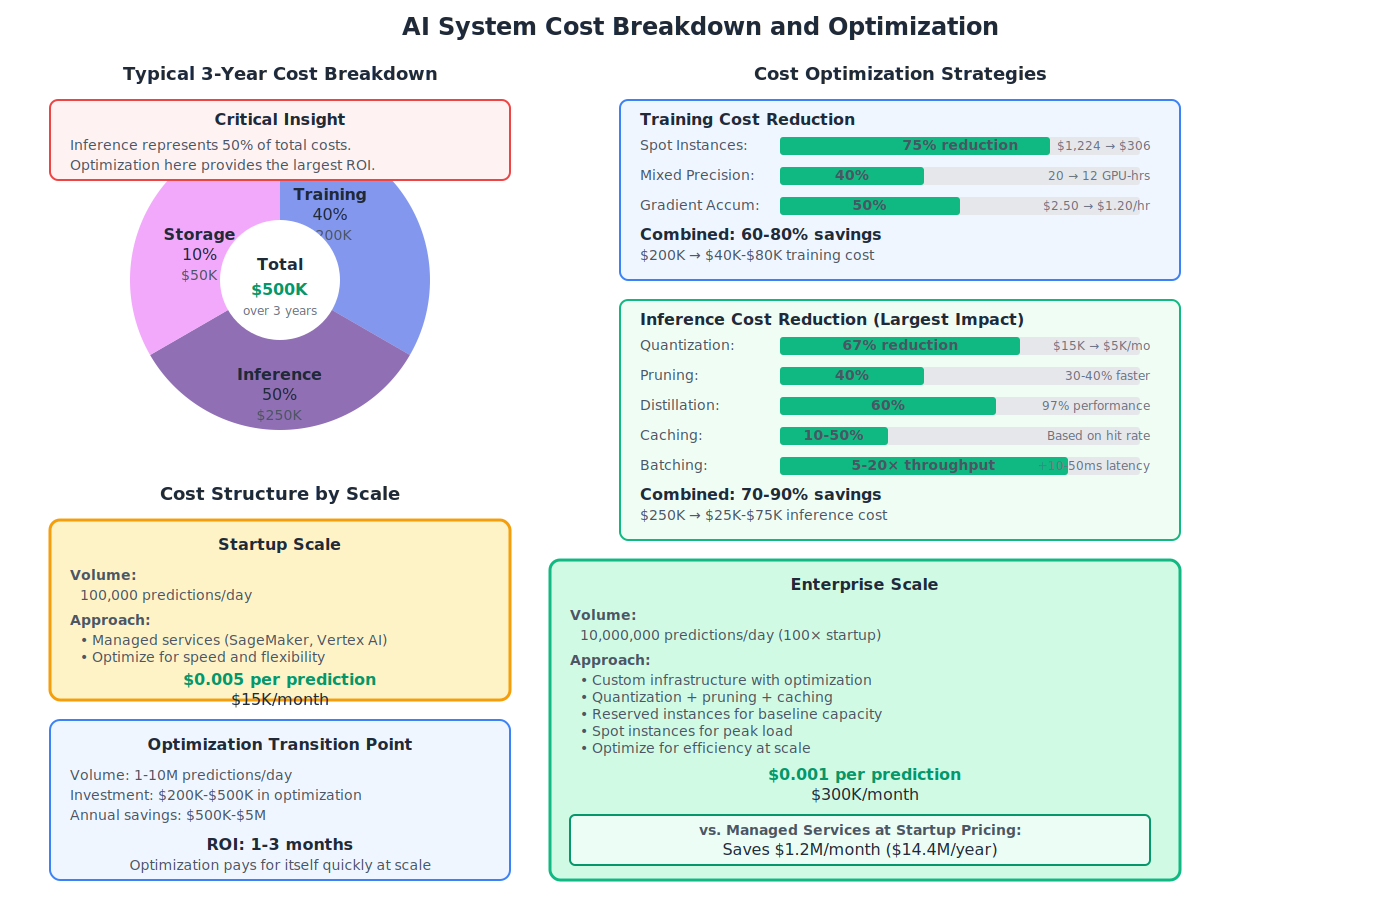
\includegraphics[width=0.95\textwidth]{chapters/diagrams/chapter09_cost_breakdown_c3d4e5f6.png}
\caption{AI system cost breakdown and optimization strategies showing typical three-year costs (40\% training, 50\% inference, 10\% storage/ops) and specific optimization techniques with quantified savings. Training optimizations (spot instances, mixed precision, gradient accumulation) provide 60-80\% savings. Inference optimizations (quantization, pruning, distillation, caching, batching) provide 70-90\% savings. The scale comparison shows the transition point where custom optimization becomes economically justified.}
\label{fig:cost_breakdown}
\end{figure}

\subsection{Startup versus Enterprise Costs}

Cost structures differ significantly between startups and enterprises. Startups typically optimize for speed and flexibility, accepting higher per-unit costs to minimize upfront investment and maintain agility. Enterprises optimize for efficiency and reliability, investing in infrastructure and automation to reduce long-term costs.

A startup serving 100,000 predictions daily might use managed services (AWS SageMaker, Google Vertex AI) at \$0.005 per prediction, costing \$15,000 monthly. This approach requires minimal engineering effort and provides instant scalability, but costs 5× more per prediction than optimized infrastructure. For early-stage startups, this trade-off makes sense: \$15,000 monthly in infrastructure costs is manageable, while the engineering effort to optimize costs (2-3 engineer-months, \$40,000-\$75,000) exceeds short-term savings.

An enterprise serving 10 million predictions daily faces different economics. At \$0.005 per prediction, costs reach \$1.5 million monthly—\$18 million annually. Investing \$200,000-\$500,000 in infrastructure optimization to reduce per-prediction costs to \$0.001 saves \$1.2 million monthly—\$14.4 million annually—providing immediate ROI. Enterprise scale justifies dedicated infrastructure, custom optimization, and operational automation.

\section*{Key Insights}

\textbf{Operational Costs Dominate Total Cost of Ownership}: Training represents 20-30\% of three-year costs; inference and operations represent 70-80\%. A model costing \$50,000 to train typically costs \$150,000-\$400,000 annually to operate. Budget planning must account for ongoing operational costs, not just initial training investment. Organizations underestimating operational costs face budget overruns and sustainability challenges.

\textbf{Model Drift Requires Systematic Retraining}: Model performance degrades over time as production data distributions shift. Degradation rates vary by domain: news and social media drift rapidly (weeks to months), e-commerce moderately (months to quarters), medical and legal slowly (quarters to years). Retraining frequency should be driven by measured performance degradation and distribution shift, not arbitrary schedules. Fine-tuning from previous versions reduces retraining costs by 80-90\% compared to training from scratch.

\textbf{Automation Provides Clear ROI at Scale}: Building automated retraining pipelines requires \$40,000-\$100,000 upfront investment but reduces per-cycle costs from \$1,000-\$3,000 to \$100-\$300. Automation breaks even after 15-30 retraining cycles, or 1.5-2.5 years for quarterly retraining. For models requiring frequent retraining or organizations managing multiple production models, automation is essential for sustainable operations.

\textbf{Security and Privacy Impose Real Costs}: Implementing differential privacy reduces accuracy by 1-5 percentage points and increases training time by 20-40\%. Adversarial training increases training costs by 20-50\%. Regulatory compliance (HIPAA, SOC 2) adds \$10,000-\$50,000 in initial setup and \$2,000-\$10,000 monthly in ongoing costs. These costs are necessary for responsible deployment and regulatory compliance, but must be factored into project budgets and ROI calculations.

\textbf{Inference Optimization Provides Largest Cost Savings}: Inference typically represents 50\% of total costs. Model compression (quantization, pruning, distillation) reduces inference costs by 50-90\% with minimal accuracy impact. Caching reduces costs by 10-50\% for systems with repeated queries. Batching increases throughput by 5-20×. Combined, these optimizations can reduce inference costs by 70-90\%, providing \$50,000-\$500,000 annual savings for production systems.

\textbf{Cost Structure Differs by Scale}: Startups optimize for speed and flexibility, accepting \$0.003-\$0.005 per prediction using managed services. Enterprises optimize for efficiency, investing in infrastructure to achieve \$0.0005-\$0.001 per prediction. The transition point occurs around 1-10 million predictions daily, where optimization investment (\$200,000-\$500,000) provides clear ROI through ongoing savings (\$500,000-\$5,000,000 annually).

\textbf{Comprehensive Monitoring Enables Optimization}: Cost monitoring and attribution—tracking cost per prediction, cost per user, cost per model version—reveals optimization opportunities and ensures budget accountability. Without detailed monitoring, cost drivers remain opaque and optimization efforts lack focus. Implementing comprehensive monitoring requires custom tagging and analysis but provides essential visibility for cost management.


% ============================================================================
% PART IV: INDUSTRY DECISION PLAYBOOK (25 pages, 7 chapters)
% ============================================================================
\part{Industry Decision Playbook}
\label{part:industry}

% Chapter 10: Hiring and Talent Development (4 pages)
\include{chapters/chapter10_hiring_talent}

% Chapter 11: Code and Developer Tools (4 pages)
\include{chapters/chapter11_code_tools}

% Chapter 12: Healthcare and Life Sciences (4 pages)
% \chapter{Healthcare and Life Sciences}

\section*{Why This Matters}

Healthcare and life sciences represent domains where transformer models address critical challenges with unique constraints rarely encountered in other industries. These constraints fundamentally shape architecture decisions, deployment strategies, and economic models. Clinical documentation consumes 30--40\% of physician time, yet proper documentation is essential for patient safety and billing. Medical imaging interpretation faces global specialist shortages amid increasing imaging volumes. Drug discovery timelines span 10--15 years at costs exceeding \$2 billion per approved drug. Patient risk prediction could prevent hospital readmissions affecting millions annually. Genomic analysis increasingly drives treatment selection but requires specialized interpretation.

Transformer-based systems demonstrate measurable impact: reducing documentation time by 50--70\%, achieving diagnostic accuracy comparable to specialists in specific imaging tasks, accelerating drug candidate identification by 2--5\times, and identifying high-risk patients for proactive intervention. Understanding these applications requires recognizing that healthcare AI success is determined not by model accuracy alone but by regulatory compliance, clinical adoption, patient outcomes, and organizational implementation—factors that do not apply uniformly across industries.

Regulatory requirements, accuracy thresholds where errors have clinical consequences, clinical workflow integration challenges, and liability frameworks create technical and operational constraints that fundamentally differ from consumer AI. This chapter examines healthcare and life sciences applications from an engineering perspective, focusing on technical requirements, regulatory constraints, economic considerations, and the adoption barriers that determine successful deployment in these high-stakes domains.

\section{Patient Risk Prediction and Clinical Decision Support}

\begin{figure}[htbp]
\centering
\includegraphics[width=0.95\textwidth]{chapters/diagrams/chapter12_risk_prediction_q1r2s3t4.png}
\caption{Patient risk prediction architecture showing the complete workflow from EHR data sources through model types to clinical applications and workflow integration. The system processes demographics, diagnoses, medications, lab values, and vital signs using gradient boosted trees, neural networks, or temporal models to predict readmission risk, sepsis, mortality, and high-cost patients. Implementation costs \$300K-1M with ROI of 0.2-5\times depending on scale and intervention effectiveness.}
\label{fig:risk_prediction_architecture}
\end{figure}

\subsection{Business Context and Applications}

Patient risk prediction represents the largest category of deployed healthcare AI, yet often receives less attention than more visible applications like imaging or drug discovery. These systems identify patients at elevated risk for adverse events, enabling proactive intervention before crises occur. The business case is compelling: preventing a single hospital readmission (average cost \$10,000--25,000) or detecting sepsis early (improving outcomes 10--15\%, worth \$5,000--15,000 per patient) justifies substantial investment in prediction systems.

Hospital readmission prediction targets patients likely to return within 30 days of discharge. Medicare estimates 15--20\% of discharged patients are readmitted within 30 days, costing the system approximately \$15 billion annually. Identifying even 30\% of high-risk readmissions and preventing 20\% of them through intervention saves organizations \$50,000+ annually per 1,000 discharges. The economic incentive is strong, particularly as Medicare reduces payment for readmissions exceeding quality thresholds.

Sepsis and acute deterioration detection systems monitor patients in real-time, identifying early warning signs of deterioration. Sepsis develops rapidly; early recognition and treatment dramatically improves survival. Studies show that one-hour delays in antibiotic administration for sepsis increase mortality by approximately 7\%. Early detection systems can alert clinicians to potential sepsis within 30--60 minutes, enabling faster treatment initiation. The value of preventing a single sepsis death (worth approximately \$100,000+ in outcome improvement) justifies substantial prediction system investment.

Mortality prediction systems estimate the probability of in-hospital or 30-day mortality, enabling conversations about goals of care, palliative care, and resource allocation. These systems enable physicians to identify when patients are unlikely to survive and have conversations about preferences before crisis occurs. The emotional and ethical value exceeds the economic value, but economic benefits also accrue through reduced unnecessary ICU days for patients with poor prognosis.

High-cost patient identification enables proactive care management targeting the 20\% of patients consuming 80\% of healthcare costs. Chronically ill patients benefit from care coordination, medication management, and remote monitoring. Identifying high-cost patients at the beginning of their engagement enables early intervention. Value is realized through reduced ER visits, hospitalizations, and complications through better disease management.

\subsection{Risk Prediction Architecture and Approaches}

Risk prediction systems typically use gradient boosted tree models or neural networks on structured patient data: demographics, diagnoses, procedures, medications, lab values, and vital signs. Electronic health records provide this data, though data extraction, cleaning, and integration often represent the largest implementation challenge.

Gradient boosted models (XGBoost, LightGBM, CatBoost) provide strong performance with advantages for healthcare deployment. These models are interpretable---feature importance rankings show which factors drive predictions---addressing a key healthcare requirement. They handle missing data well, which is critical for EHR data with inconsistent documentation. They are computationally efficient, enabling real-time prediction in clinical systems. The trade-off involves lower performance compared to deep learning models.

Neural network models on structured data achieve 3--8\% better performance than gradient boosted models but with reduced interpretability. Attention mechanisms can highlight which data points most influence predictions, providing some interpretability. For complex datasets with thousands of features and long history, neural networks can learn nonlinear interactions that tree models miss.

Temporal models (recurrent neural networks, temporal convolutional networks) explicitly model time series aspects of patient data: lab values changing over time, medication adjustments, symptom progression. These models naturally capture disease trajectories and deterioration patterns better than models treating all data as a single snapshot. The trade-off involves greater complexity and computational cost.

\subsection{Clinical Validation and Adoption Challenges}

Risk prediction systems require careful clinical validation. High-performing models in development often show reduced performance when deployed to new hospital systems or patient populations. This performance degradation occurs because training data may not represent deployment data: patient mix differs, documentation practices vary, hospital workflows differ, and underlying disease prevalence varies.

Prospective validation studies, where the system makes predictions on new patients before clinical outcomes are known, provide the strongest evidence. These studies demonstrate whether the system actually predicts future outcomes. Retrospective studies on historical data cannot account for changes in clinical practice, documentation, or patient mix over time.

Adopting risk prediction requires integrating with clinical workflows and EHR systems. Ideal integration places predictions in the workflow where clinicians naturally encounter information: admission summaries, shift handoffs, clinical dashboards. Predictions that require clinicians to check a separate system rarely achieve high utilization. Alert fatigue is a significant risk---clinicians may ignore systems that generate frequent alerts, even if most are accurate. Typical recommendation is that alerts should have positive predictive value exceeding 50\% for adoption; lower thresholds generate alert fatigue.

Physician acceptance depends on trust and clinical validation. Clinicians want to understand why a system made a prediction and whether they agree. Models that simply output a risk score without explanation face skepticism. Explanation methods showing which factors most influenced a prediction help clinicians evaluate prediction reasonableness.

\subsection{Economic Impact and Implementation}

The economic value of risk prediction depends on the specific application and effectiveness of interventions. For readmission prediction, preventing one readmission (cost \$10,000--25,000) through intervention generates value. If a system identifies 100 high-risk patients and 30 would have been readmitted, preventing 20\% of those through intervention saves \$60,000 (6 prevented readmissions at \$10,000 average). At \$50,000 annual system cost, ROI is marginal unless volume is higher or prevention rates are better.

For sepsis detection with one-hour earlier identification, value reaches \$5,000--15,000 per patient detected (improved survival times reduced ICU duration). Detecting 50 sepsis cases annually with 30\% improvement rate and average \$10,000 value yields \$150,000 in annual value, supporting system cost of \$30,000--50,000 monthly.

Implementation costs include EHR integration (6--12 months, \$100,000--300,000), data infrastructure (extracting, cleaning, updating patient data in real-time), model validation (clinical studies demonstrating effectiveness), and monitoring (tracking prediction accuracy over time). Total implementation cost typically reaches \$300,000--1,000,000 for health systems. This capital investment requires strong business case and executive support.

Infrastructure costs for serving prediction models at scale are modest. Scoring 10,000 patient records daily against multiple prediction models requires minimal compute: a few CPU cores suffice. The bottleneck is data extraction and integration with EHRs, not model inference.

Continuous improvement is essential for sustained success. Patient populations change, documentation practices evolve, and disease epidemiology shifts seasonally. Models that remain static degrade in performance over months. Retraining models on recent data maintains performance but requires sustained investment and governance.

\section{Clinical Natural Language Processing}

\begin{figure}[htbp]
\centering
\includegraphics[width=0.95\textwidth]{chapters/diagrams/chapter12_clinical_nlp_a1b2c3d4.png}
\caption{Clinical NLP pipeline for documentation assistance, showing the end-to-end workflow from patient-physician conversation through speech recognition, information extraction with Clinical BERT, note generation, physician review, and EHR integration. The system achieves 90-95\% accuracy and reduces documentation time by 50-70\%, providing 3-10\times ROI.}
\label{fig:clinical_nlp_pipeline}
\end{figure}

\subsection{Clinical Text Characteristics and Domain-Specific Challenges}

Clinical documentation differs fundamentally from general text in ways that affect model architecture and training strategies. Medical terminology includes highly specialized vocabulary---anatomical terms, drug names, procedure codes, disease classifications---that rarely appears in general corpora. A single clinical note might contain hundreds of domain-specific terms that general-purpose language models have never encountered during training.

Abbreviations and acronyms appear with extreme density in clinical text. ``PT'' might mean patient, physical therapy, prothrombin time, or posterior tibial, depending on context. ``MS'' could indicate multiple sclerosis, mitral stenosis, mental status, or morphine sulfate. Disambiguation requires medical knowledge and contextual understanding that general models lack. Clinical NLP systems must handle this ambiguity reliably, as misinterpretation directly affects patient care.

Temporal reasoning pervades clinical documentation. Understanding disease progression, treatment response, and medication timing requires tracking events across multiple notes spanning months or years. A phrase like ``improved since last visit'' requires identifying the previous visit, extracting relevant findings, comparing current state, and understanding the temporal relationship. This temporal reasoning exceeds the capabilities of models processing individual notes in isolation.

Negation and uncertainty require careful handling. ``No evidence of pneumonia'' means the opposite of ``evidence of pneumonia,'' yet both contain the word ``pneumonia.'' ``Possible cardiac involvement'' expresses uncertainty that affects clinical decision-making differently than ``confirmed cardiac involvement.'' Clinical NLP systems must detect and preserve these semantic distinctions, as errors directly lead to inappropriate treatment decisions.

\subsection{Clinical Language Models and Training Requirements}

Specialized clinical language models address domain-specific challenges through targeted pre-training on medical text. Clinical BERT, trained on 2 million clinical notes from MIMIC-III, achieves 3--5\% better performance than general BERT on clinical NLP tasks such as medication extraction and adverse event detection. This improvement, while seemingly modest, translates to thousands of correctly processed notes in production deployment.

BioBERT and PubMedBERT target biomedical literature rather than clinical notes, training on PubMed abstracts and full-text articles. These models excel at scientific text understanding---extracting relationships between genes, proteins, and diseases---but perform worse on clinical documentation with its abbreviations and informal language. Model selection depends on the specific application: clinical documentation assistance versus biomedical research literature analysis.

Model size for clinical applications typically ranges from 110 million to 340 million parameters (BERT-base to BERT-large). Larger models provide better performance but face deployment constraints in healthcare IT environments with limited GPU resources and conservative IT governance. Many healthcare organizations lack the infrastructure for serving multi-billion parameter models, making smaller, efficient models more practical despite lower absolute performance.

Fine-tuning clinical models requires labeled clinical data. Clinical experts---physicians, nurses, medical coders---must annotate training examples, costing \$50--200 per hour depending on specialization and task complexity. Annotating 10,000 examples for a clinical NLP task costs \$100,000--500,000. This annotation cost often exceeds model training costs, making data efficiency critical for economic viability. Organizations should carefully define annotation scope, provide detailed guidelines, and validate inter-annotator agreement before scaling annotation efforts.

\subsection{Clinical NLP Applications and Economic Value}

Clinical documentation assistance represents the highest-impact application, addressing physician burnout from documentation burden. Ambient clinical intelligence systems listen to patient-physician conversations, extract relevant information through speech-to-text and NLP, and generate clinical note drafts. These systems reduce documentation time from 2--3 hours daily to 30--60 minutes, enabling physicians to see more patients or recover working hours.

Implementation requires careful attention to accuracy and clinical workflow integration. The system must correctly capture diagnoses, medications, allergies, and treatment plans, as errors directly affect patient safety. Physicians must review and edit generated notes---notes are not simply accepted but refined. Typical accuracy targets are 90--95\% for structured information extraction (diagnoses, medications), with physician review catching remaining errors and adding nuance.

Clinical coding---assigning ICD-10 diagnosis codes and CPT procedure codes for billing---represents another application. Manual coding by certified coders costs \$2--5 per encounter. Automated coding systems achieve 70--85\% accuracy on common diagnoses and procedures, with human coders reviewing and correcting predictions. This hybrid approach reduces coding costs by 40--60\% while maintaining billing accuracy and compliance.

Clinical decision support systems extract information from clinical notes to identify patients at risk for specific conditions or complications. A system might scan notes to identify patients with uncontrolled diabetes, overdue cancer screenings, or drug interaction risks. These systems must achieve high recall (finding all relevant cases) while maintaining acceptable precision (avoiding false alarms). Typical targets are 85--95\% recall and 70--85\% precision.

Economic analysis for clinical documentation assistance is compelling. A physician earning \$200,000--400,000 annually spending 30--40\% of time on documentation represents \$60,000--160,000 annual cost. Reducing documentation time by 60\% saves \$36,000--96,000 per physician. At \$10,000--30,000 annual system cost per physician, ROI is 2--10\times. Implementation across 100 physicians saves \$3.6--9.6 million annually, supporting substantial investment.

\section{Medical Imaging and Computer Vision}

\begin{figure}[htbp]
\centering
\includegraphics[width=0.95\textwidth]{chapters/diagrams/chapter12_medical_imaging_e5f6g7h8.png}
\caption{Multimodal medical imaging architecture combining vision transformers for image processing with Clinical BERT for text encoding. Cross-attention mechanisms enable fusion of visual and clinical context, achieving 5-10\% better accuracy than image-only models. The system requires 8-16 GB GPU memory for inference and must undergo FDA validation.}
\label{fig:medical_imaging_architecture}
\end{figure}

\subsection{Vision Transformers for Medical Imaging}

Medical imaging applications---radiology, pathology, dermatology, ophthalmology---face global specialist shortages and increasing imaging volumes. Vision transformers applied to medical images achieve diagnostic accuracy comparable to specialists for specific, well-defined tasks: detecting pneumonia on chest X-rays (95\%+ accuracy), identifying diabetic retinopathy in fundus photographs (90\%+ accuracy), or classifying skin lesions.

Medical images differ from natural images in ways that affect model architecture. Images are often high-resolution (2000\times2000 pixels or larger for CT/MRI), grayscale or specialized color spaces (for different imaging modalities), and contain subtle features critical for diagnosis. A 2mm lung nodule in chest CT might be the only sign of early cancer, requiring models to detect tiny features in large images.

Vision transformer architectures for medical imaging use patch sizes of 16\times16 or 32\times32 pixels, dividing a 2000\times2000 image into 3,900--15,600 patches. Processing this many patches requires substantial memory and computation. A ViT-Large model processing a 2000\times2000 image requires approximately 24 GB of memory during training, necessitating high-end GPUs or gradient checkpointing techniques. Alternative architectures (Swin transformers, hierarchical approaches) reduce computational requirements by processing images at multiple resolutions.

Transfer learning from natural images (ImageNet pre-training) provides limited benefit for medical imaging. ImageNet pre-training helps with general visual features (edges, textures) but doesn't capture medical-specific patterns (lung infiltrates, cellular morphology, tissue density variations). Domain-specific pre-training on medical image datasets (ChestX-ray14, MIMIC-CXR) provides better performance. These medical datasets are smaller than ImageNet, limiting pre-training benefits, but the domain-specific knowledge justifies pre-training.

\subsection{Modality-Specific Considerations}

Radiology applications (X-ray, CT, MRI, ultrasound) have different characteristics affecting model architecture and deployment. X-ray is two-dimensional, high-volume (100+ per radiologist daily), and relatively fast to interpret. AI systems can process X-rays quickly, enabling throughput increases. CT and MRI are three-dimensional, requiring models to process volumetric data (10\times more data than 2D). Processing 3D data requires either volumetric neural networks (computationally expensive) or 2D slice-by-slice approaches (missing 3D context).

Pathology deals with gigapixel images (40,000\times40,000 pixels or larger) from slide scanners. Standard image processing approaches fail because the entire image doesn't fit in GPU memory. Specialized approaches divide images into tiles, process tiles independently, then aggregate results. These approaches must handle tile boundaries carefully to avoid missing structures spanning multiple tiles.

Dermatology faces different challenges. Standardized photography is critical---lighting, angle, and distance affect appearance. Variability in photography makes models less reliable. However, clinical stakes are typically lower (skin conditions are rarely life-threatening), and treatment decisions are often clear. Dermatology AI adoption is relatively high because risk is low and benefit is clear.

Ophthalmology involves specialized imaging equipment (fundus cameras, optical coherence tomography) producing images optimized for specific diseases. Models trained on fundus images for diabetic retinopathy may not generalize to other retinal diseases. Modality-specific training data is essential.

\subsection{Multimodal Clinical Models}

Combining medical images with clinical text enables richer understanding than either modality alone. A chest X-ray interpreted with the patient's clinical history, symptoms, and prior imaging provides more accurate diagnosis than the image alone. Multimodal models that process both images and text achieve 5--10\% better diagnostic accuracy than image-only models.

Architecture for multimodal models typically uses separate encoders for each modality---a vision transformer for images, a language model for text---with cross-attention mechanisms enabling interaction. The text encoder processes clinical history, prior reports, and symptom descriptions. The vision encoder processes the current image. Cross-attention allows the model to focus on image regions relevant to mentioned symptoms or findings.

Training multimodal models requires paired image-text data. Radiology reports paired with images provide natural training data, but report quality varies. Some reports are detailed and specific; others are brief and generic. Data curation to identify high-quality image-report pairs improves model performance but requires clinical expertise.

Computational requirements exceed single-modality models. Processing a 2000\times2000 image with a 500-token clinical history requires approximately 32 GB of memory during training. Inference requires 8--16 GB. These resource requirements necessitate GPU deployment for real-time clinical use.

\subsection{Clinical Deployment and Regulatory Requirements}

Medical imaging AI systems require FDA approval as medical devices under the Software as Medical Device (SaMD) framework. This regulatory requirement involves demonstrating safety and effectiveness through clinical studies with hundreds to thousands of cases. Validation costs \$500,000--2,000,000 and takes 12--24 months, substantially increasing time-to-market and development costs.

Clinical validation requires demonstrating performance on diverse patient populations, imaging equipment, and clinical settings. A model trained on academic medical center data might perform poorly on images from community hospitals with different equipment or patient demographics. Validation datasets must represent the intended use population, requiring multi-site data collection and careful attention to demographic diversity.

Continuous monitoring after deployment detects performance degradation. Imaging equipment changes, patient populations shift, and disease epidemiology varies over time. These changes degrade model performance, requiring retraining or recalibration. Monitoring systems track prediction confidence, error rates, and distribution shift, alerting when performance falls below acceptable thresholds.

Liability and responsibility frameworks affect deployment. If an AI system misses a diagnosis, who is liable---the physician, healthcare organization, or AI vendor? Current practice treats AI as decision support, with physicians retaining ultimate responsibility. This framework requires physicians to review and validate AI predictions, limiting automation potential. As confidence in AI systems increases, liability frameworks will evolve, potentially enabling greater automation with appropriate safeguards.

\section{Genomics and Precision Medicine}

\subsection{Genetic and Genomic AI Applications}

Genomic analysis increasingly drives clinical decisions: identifying pathogenic genetic variants, determining cancer mutation profiles that guide treatment selection, and assessing pharmacogenomic variants that affect drug metabolism. Transformer models and other machine learning approaches are being applied to genetic data with increasing clinical impact.

Variant interpretation---determining whether a genetic variant is pathogenic, benign, or uncertain---is a critical bottleneck. Clinically actionable genetic testing produces thousands of variants per patient, most of which are benign. Computational tools must prioritize which variants deserve expert review. Machine learning models trained on databases of known pathogenic variants (ClinVar, HGMD) predict pathogenicity of novel variants. Performance reaches 85--92\% accuracy on well-studied genes.

Cancer genomics has transformed clinical oncology. Tumor sequencing identifies mutations in cancer-causing genes, determining which treatments are likely effective. For example, mutations in EGFR in lung cancer predict response to specific targeted therapies; mutations in BRCA1/2 affect breast cancer treatment strategy. Machine learning predicts treatment response from mutation profiles with 75--85\% accuracy.

Pharmacogenomics analyzes genetic variants affecting drug metabolism. Variations in cytochrome P450 enzymes determine whether patients metabolize certain drugs quickly (requiring higher doses) or slowly (risking toxicity). Genetic testing predicts optimal dosing for many medications. The economic value is high: preventing adverse drug events costs \$5,000--20,000 per event avoided.

Rare disease diagnosis uses genetic variants to match patients to disease causes. Rare genetic diseases often have multiple possible causes; genetic sequencing identifies mutations and machine learning determines most likely diagnosis. This genetic diagnosis enables appropriate treatment and prognosis counseling.

\subsection{Technical Approaches and Validation}

Machine learning approaches for genomic analysis range from sequence-based (processing DNA sequences directly) to variant-based (processing individual genetic variants) to multi-omics (combining genomic, transcriptomic, proteomic data).

Sequence-based approaches use language models trained on DNA sequences. DNA can be represented as text (A, T, G, C nucleotides), enabling direct application of NLP methods. Nucleotide transformers trained on billions of base pairs learn sequence patterns associated with function and disease. These models predict mutation effects, pathogenic variants, and regulatory changes from sequence alone.

Variant-based approaches treat individual genetic variants as features. A patient is represented as a vector of presence/absence of specific variants. Gradient boosted models or neural networks predict phenotypes (disease presence, treatment response) from variant profiles. These approaches are computationally simpler than sequence-based approaches but don't leverage the information in variant context.

Multi-omics approaches combine genomic, transcriptomic (which genes are expressed), proteomic (protein abundance), and metabolomic (chemical byproducts) data. Integration of these data types provides richer understanding of disease biology. Transformer-based multi-omics models achieve better disease prediction than single-omics approaches.

Regulatory requirements for genomic AI are evolving. CLIA (Clinical Laboratory Improvement Amendments) governs clinical genetic testing. FDA oversight of genomic AI is increasing for high-stakes applications (cancer diagnosis, pharmacogenomics). HIPAA requirements apply as genetic data is part of medical records. Regulatory landscape is complex and changing, requiring careful monitoring.

\subsection{Economic Impact and Adoption}

Economic value of genomic AI depends on the specific application. Variant interpretation reduces time spent on manual curation: experts reviewing variants manually cost \$100--500 per variant. Automated interpretation with 85\%+ accuracy reduces expert time by 80\%, saving \$80--400 per variant. For a diagnostic lab processing 10,000 variants annually, savings reach \$800,000--4,000,000.

Cancer genomics AI guiding treatment selection enables better outcomes and cost optimization. Patients receiving treatment matched to their tumor profile see better response rates and fewer adverse effects. Value per correct prediction: \$20,000--100,000 (improved survival, reduced unnecessary treatment).

Pharmacogenomics testing prevents adverse drug events with value of \$5,000--20,000 per event prevented. For a population on multiple medications, genetic testing could prevent 5--10 adverse events per 1,000 patients annually. At \$100 per test, costs are offset within a year.

\section{Drug Discovery and Molecular Design}

\begin{figure}[htbp]
\centering
\includegraphics[width=0.95\textwidth]{chapters/diagrams/chapter12_drug_discovery_i9j0k1l2.png}
\caption{AI-driven drug discovery workflow showing the complete pipeline from target identification through molecular generation, virtual screening, experimental validation, and lead optimization. The iterative process reduces discovery timelines from 3-5 years to 1-2 years, providing \$200-400M savings per successful drug with 10-80\times ROI for successful programs.}
\label{fig:drug_discovery_workflow}
\end{figure}

\subsection{Molecular Representation and Property Prediction}

Drug discovery applications use transformers to model molecular structures and predict properties. Molecules can be represented as SMILES strings (text notation), molecular graphs, or 3D conformations. Each representation has different characteristics affecting model architecture.

SMILES (Simplified Molecular Input Line Entry System) represents molecules as text strings, enabling direct application of language models. The SMILES string ``CC(=O)OC1=CC=CC=C1C(=O)O'' represents aspirin. Language models trained on SMILES strings learn chemical grammar and generate novel molecules. However, SMILES has limitations: multiple SMILES strings can represent the same molecule, and small string changes can produce very different molecules.

Graph neural networks treat molecules as graphs with atoms as nodes and bonds as edges. Graph transformers apply attention to molecular graphs, learning relationships between atoms. This representation naturally captures molecular structure.

Property prediction estimates a molecule's solubility, toxicity, binding affinity, or metabolic stability. Models trained on molecular property databases achieve correlation coefficients of 0.7--0.9 with experimental measurements for well-studied properties. This accuracy enables virtual screening of millions of candidates, identifying promising molecules for experimental testing.

\subsection{Generative Models for Drug Design}

Generative models create novel molecular structures with desired properties, accelerating lead compound identification. These models learn the distribution of drug-like molecules from databases of known drugs and bioactive compounds, then generate new molecules from this learned distribution.

Conditional generation targets specific properties. A model might generate molecules with high binding affinity to a target protein, low toxicity, and favorable pharmacokinetics. Multi-objective optimization is challenging, as properties often trade off: molecules with high binding affinity might have poor solubility.

Validation requires experimental testing. Synthesizing and testing a single compound costs \$5,000--50,000 and takes weeks to months. Generative models must achieve high hit rates---the fraction of generated molecules showing desired activity---to justify experimental costs. Current models achieve 5--20\% hit rates for well-defined targets, versus 0.1--1\% random screening.

Integration with experimental workflows determines practical impact. Generative models producing molecules difficult or impossible to synthesize provide limited value. Synthetic accessibility constraints during generation---favoring molecules synthesizable with available chemistry---improves utility. This requires combining learned models with rule-based chemical knowledge.

\subsection{Protein Structure and Design Applications}

Protein language models, trained on millions of protein sequences, learn relationships between sequence and structure. ESM-2, trained on 250 million protein sequences, achieves state-of-the-art protein structure prediction and function annotation from sequence alone.

Protein structure prediction, exemplified by AlphaFold2's revolutionary results, uses transformer-based architectures to predict 3D structure from amino acid sequence. While AlphaFold2 uses specialized architectures beyond standard transformers, the attention mechanism is central. Accurate structure prediction enables drug discovery by identifying binding sites and predicting drug-protein interactions computationally.

Antibody design applies transformers to generate antibody sequences with desired binding properties. Antibodies are proteins with variable regions determining binding specificity. Generative models trained on antibody sequence databases design novel antibodies targeting specific antigens, accelerating therapeutic antibody development.

\subsection{Impact on Drug Discovery Timelines and Economics}

Drug discovery traditionally spans 10--15 years and costs exceeding \$2 billion per approved drug. This timeline breaks down roughly as: 3--6 years target identification and lead optimization (preclinical), 6--7 years clinical trials (Phase I, II, III), and 1--2 years FDA review. AI can dramatically accelerate preclinical stage, potentially reducing it from 3--6 years to 1--2 years. Clinical trials, which represent the majority of cost and timeline, are much harder to accelerate.

Preclinical time savings directly reduce time-to-first-human-trial, accelerating revenue generation for successful drugs. A two-year reduction in preclinical time, with appropriate discounting for time value of money and success rate changes, can be worth \$200--400 million per successful drug through reduced pre-revenue costs and earlier revenue start.

Hit rate improvements (finding more promising candidates earlier) reduce experimental costs and increase probability of advancing to clinical trials. If AI enables 20\% improvement in early-stage hit rates, this reduces the number of compounds requiring expensive synthesis and testing.

However, clinical trials remain expensive and time-consuming regardless of AI progress. Phase III trials for major indications cost \$400--1000 million and take 2--4 years, depending on indication and required patient population. AI can improve trial design (patient selection, endpoint selection) but cannot eliminate the fundamental requirement for human data.

\section{Implementation and Governance}

\subsection{Healthcare IT Integration and Deployment}

Healthcare AI systems must integrate with complex IT infrastructure: electronic health records, picture archiving systems, laboratory systems, pharmacy systems, and clinical workflows. Integration complexity often exceeds model development complexity, consuming 60--80\% of deployment effort.

EHR integration requires handling diverse data formats, inconsistent data quality, and vendor-specific APIs. Epic, Cerner, and other vendors provide different integration mechanisms with varying capabilities. HL7 FHIR standards improve interoperability but adoption remains incomplete. Integration projects require 6--12 months of engineering effort.

Real-time requirements for clinical decision support create latency constraints. Systems alerting physicians to drug interactions must respond within seconds to avoid disrupting workflow. Batch processing overnight suffices for population analytics but not for point-of-care support.

Data privacy and security exceed typical enterprise standards. HIPAA mandates encryption, access controls, audit logging, and breach procedures. Cloud deployment requires Business Associate Agreements with providers. These requirements add complexity and cost.

\subsection{Clinical Validation and Regulatory Approval}

Clinical validation requires demonstrating that AI systems improve patient outcomes. A model with 95\% accuracy might not improve outcomes if physicians don't trust or act on predictions.

Randomized controlled trials provide strongest evidence but are expensive and time-consuming: \$1--5 million, 12--24 months. Observational studies are faster and cheaper but weaker: \$100,000--500,000, 6--12 months.

Publication in peer-reviewed journals establishes credibility before clinical adoption. The publication process adds 6--12 months to evidence generation timelines.

Reimbursement codes and payer negotiations determine financial viability. Without reimbursement, healthcare organizations lack financial incentive to adopt.

\subsection{Fairness, Bias, and Equity}

Healthcare AI models often exhibit bias across demographic groups. Models trained predominantly on one demographic perform worse on others. Historical bias in training data encodes past discrimination. This affects equitable access to AI benefits.

Fairness metrics and mitigation strategies are critical. Sensitivity and specificity may differ across demographic groups; equity requires understanding and addressing these differences.

FDA guidance increasingly requires algorithmic fairness assessment. Demonstrating equitable performance across demographic groups becomes part of regulatory approval.

Monitoring after deployment should track performance across demographic groups, alerting when disparities emerge. This requires collecting demographic data and analyzing performance stratified by demographics.

\subsection{Operational Monitoring and Continuous Improvement}

Deployed systems degrade over time as patient populations change, disease epidemiology shifts, and clinical practices evolve. Continuous monitoring detects performance degradation and triggers retraining.

Monitoring infrastructure tracks prediction accuracy, confidence distributions, and error patterns. Alerts trigger when performance falls below thresholds.

Model monitoring costs approximate 10--20\% of initial development cost annually, making it essential to budget for sustained operations, not just initial deployment.

Continuous improvement processes collect feedback from clinical users, identify failure modes, and improve models. This organizational capability determines long-term success more than initial model quality.

\section{Economic Analysis and Return on Investment}

\begin{figure}[htbp]
\centering
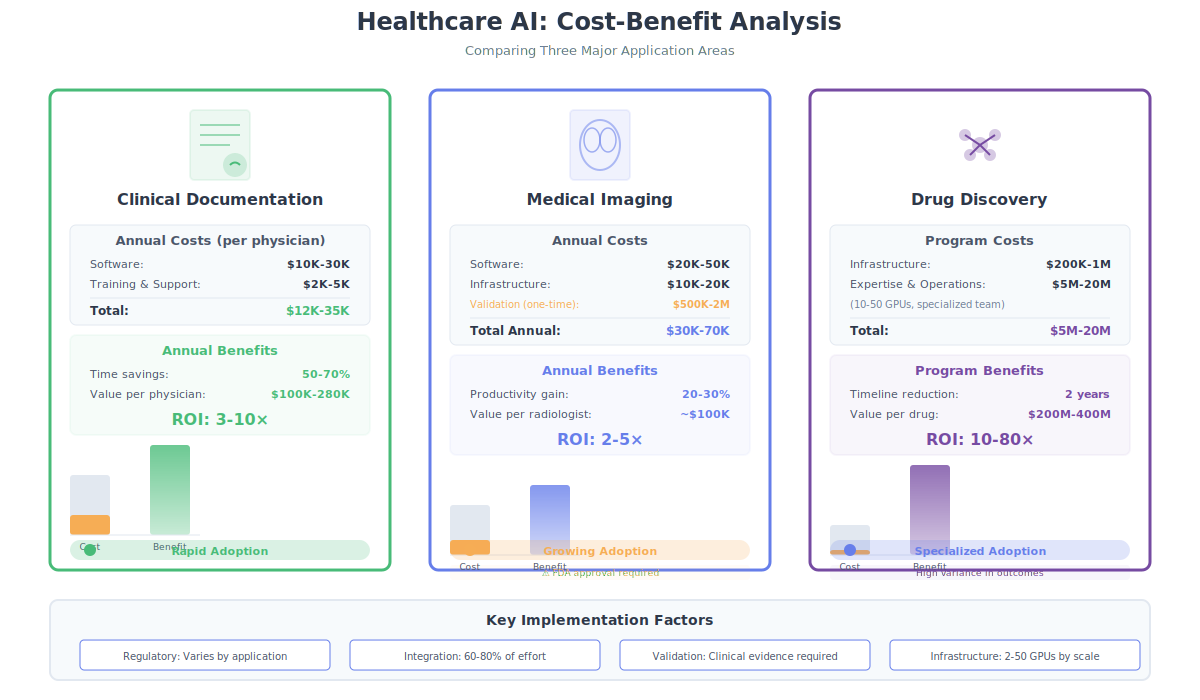
\includegraphics[width=0.95\textwidth]{chapters/diagrams/chapter12_cost_benefit_m3n4o5p6.png}
\caption{Cost-benefit analysis comparing three major healthcare AI applications. Clinical documentation provides the highest adoption rate with 3-10\times ROI at \$12K-35K annual cost per physician. Medical imaging requires FDA approval and provides 2-5\times ROI. Drug discovery demands \$5M-20M investment but offers 10-80\times ROI for successful programs with high outcome variance.}
\label{fig:healthcare_cost_benefit}
\end{figure}

Healthcare AI economics are application-specific, with wide variation in ROI and implementation complexity.

\textbf{Patient risk prediction}: \$50,000--500,000 annual value per health system (depending on scale and intervention effectiveness) at \$100,000--300,000 implementation cost. ROI is 0.2--5\times depending on scale and success of interventions. Implementation complexity is medium. Value is sustained with proper monitoring and continuous improvement.

\textbf{Clinical documentation}: \$3.6--9.6 million annual value for 100 physicians (per physician savings) at \$1--3 million implementation cost. ROI is 2--10\times. Implementation complexity is high due to workflow integration. Value is immediate upon deployment with rapid adoption.

\textbf{Medical imaging}: \$100,000 annual value per radiologist (25\% productivity improvement) at \$50,000--100,000 implementation cost. ROI is 1--2\times per radiologist, with compounding benefits across radiology departments. Implementation complexity is medium. FDA approval adds 12--24 months and \$500,000--2,000,000 cost but is mandatory for clinical deployment.

\textbf{Drug discovery}: \$200--400 million value per successful drug (through timeline compression and success rate improvement) at \$5--20 million investment in AI platform and expertise. ROI is 10--80\times for successful programs, but outcome variance is high---unsuccessful programs yield minimal return. Implementation complexity is high; scientific expertise required.

\textbf{Genomic analysis}: \$500,000--4,000,000 annual value in reduced interpretation costs at \$100,000--500,000 implementation cost. ROI is 1--40\times depending on application and volume. Implementation complexity is medium.

Infrastructure costs vary by application. Clinical NLP and risk prediction require modest compute (standard servers with GPUs). Medical imaging requires 4--8 GPUs for enterprise deployment. Drug discovery platforms require 10--50 GPUs. Monthly cloud costs range from \$1,000 to \$25,000 depending on application.

\section{Key Insights}

\textbf{Patient Risk Prediction is the Largest Deployed Category}: While imaging and drug discovery attract attention, risk stratification systems are deployed at scale across healthcare organizations. Identifying high-risk patients enables proactive intervention, preventing readmissions and adverse events. This category deserves equivalent emphasis to more visible applications.

\textbf{Domain Specialization is Essential}: General-purpose models perform poorly on clinical text due to specialized terminology, dense abbreviations, and medical reasoning. Clinical BERT and biomedical models achieve 3--5\% better performance than general models, translating to thousands of correctly processed notes in production.

\textbf{Integration and Workflow Complexity Determine Success}: Technical model quality is necessary but insufficient. Integration with EHRs, PACS, clinical workflows, and identity systems consumes 60--80\% of effort. Deployment success depends more on integration execution than on model performance.

\textbf{Regulatory Requirements Dominate Timelines}: FDA approval for medical devices requires 12--24 months and costs \$500,000--2,000,000. Clinical validation and evidence generation consume 60--80\% of total development effort. Organizations should budget appropriately for regulatory pathways.

\textbf{Accuracy Thresholds are Non-Negotiable}: Healthcare applications require 90--95\% accuracy for clinical use, as errors directly affect patient safety. This accuracy requirement necessitates extensive validation, human review workflows, and continuous monitoring.

\textbf{Economic Value Varies Dramatically by Application}: Clinical documentation provides 2--10\times ROI through physician time savings. Medical imaging provides 1--2\times ROI per radiologist. Drug discovery provides 10--80\times ROI for successful programs with high outcome variance. Risk prediction provides 0.2--5\times ROI depending on scale and intervention success. Organizations should evaluate each application on its specific economics.

\textbf{Physician Adoption is the Largest Barrier}: Even highly accurate systems fail to deliver value if physicians don't trust or use them. Building trust requires clinical validation, transparency in model decision-making, and seamless workflow integration. Adoption timelines extend 6--12 months beyond technical deployment.

\textbf{Fairness and Equity Matter for Both Ethics and Regulation}: Healthcare AI systems often exhibit performance disparities across demographic groups. Regulatory bodies increasingly require fairness assessment. Organizations should monitor performance across groups and implement bias mitigation strategies.

\textbf{Continuous Monitoring and Improvement are Essential}: Deployed systems degrade over time. Continuous monitoring, periodic retraining, and adaptation to changing clinical conditions sustain value. Budget for ongoing operations approximating 10--20\% of initial development cost annually.

The next chapter examines legal and compliance applications, where transformer models address document review, contract analysis, and regulatory compliance with unique accuracy and explainability requirements fundamentally different from healthcare's clinical validation paradigm.



% Chapter 13: Legal and Compliance (4 pages)
% \chapter{Legal and Compliance}

\section*{Why This Matters}

Legal and compliance applications represent domains where transformer models address document-intensive workflows with stringent accuracy and explainability requirements fundamentally different from general-purpose AI. These requirements create unique technical and operational challenges. Contract review consumes 30--50\% of associate attorney time. Regulatory compliance requires continuous analysis of evolving regulations across multiple jurisdictions. Legal research involves synthesizing information from millions of case documents. Due diligence in mergers and acquisitions must review thousands of contracts and financial documents within compressed timelines. Financial compliance includes monitoring transactions for suspicious activity and sanctions violations.

Transformer-based systems demonstrate measurable impact: reducing contract review time by 40--60\%, identifying compliance risks with 85--95\% accuracy, and accelerating legal research by 3--5\times. However, success in these domains is determined not by model accuracy alone but by explainability, professional responsibility compliance, integration with existing workflows, and robust quality assurance.

Understanding legal AI applications requires recognizing constraints that distinguish this domain. Explainability requirements where decisions must be justified with specific citations to source documents. Liability considerations where errors can result in multi-million dollar consequences. Professional responsibility standards that maintain attorney oversight and ultimate responsibility for work product. These constraints fundamentally shape technical architecture decisions and deployment strategies.

This chapter examines legal and compliance applications from an engineering perspective, focusing on the technical requirements, explainability constraints, and risk management considerations that determine successful deployment in these high-stakes professional domains.

\section{Contract Analysis and Review}

\begin{figure}[htbp]
\centering
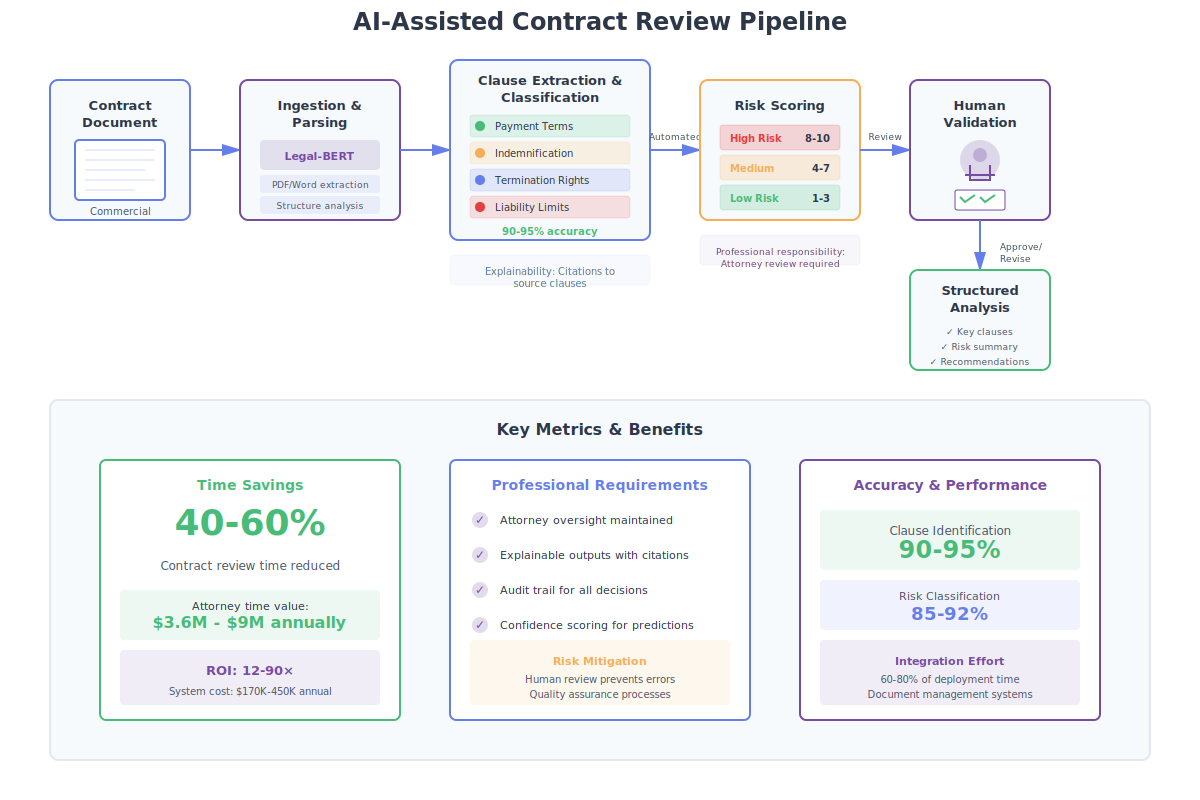
\includegraphics[width=0.95\textwidth]{chapters/diagrams/chapter13_contract_review_a1b2c3d4.png}
\caption{AI-assisted contract review pipeline showing the complete workflow from document ingestion through Legal-BERT processing, clause extraction and classification, risk scoring, attorney validation, and structured analysis output. The system achieves 90-95\% accuracy for clause identification and provides 40-60\% time savings with 12-90× ROI while maintaining required attorney oversight.}
\label{fig:contract_review_pipeline}
\end{figure}

\subsection{Contract Document Characteristics}

Legal contracts differ from general documents in ways that affect model architecture and training strategies. Contracts contain highly structured language with specific legal terminology, defined terms that carry precise meanings within the document, and cross-references creating complex dependency relationships. A single contract might reference dozens of defined terms, each requiring consistent interpretation throughout.

Clause identification and classification require understanding legal concepts and document structure. Standard clauses---indemnification, limitation of liability, termination rights---appear with variations across contracts. Models must recognize semantic equivalence despite syntactic differences: ``Party A shall indemnify Party B'' and ``Party B shall be held harmless by Party A'' express similar obligations despite different wording.

Temporal and conditional logic pervades contract language. Obligations often depend on specific conditions, dates, or events: ``If Party A fails to deliver within 30 days, Party B may terminate.'' Understanding these dependencies requires parsing complex conditional structures and tracking temporal relationships across multiple clauses. Errors in temporal reasoning lead to misidentifying obligations or missing critical deadlines.

Ambiguity detection represents a critical capability for contract review. Vague terms like ``reasonable efforts,'' ``material breach,'' or ``commercially reasonable'' create interpretation risks. Models must identify potentially ambiguous language and flag it for attorney review, as ambiguity often becomes the subject of disputes. This requires understanding not just what text says, but what it fails to specify clearly.

\subsection{Contract Review Models and Approaches}

Specialized legal language models address domain-specific challenges through pre-training on legal corpora. Legal-BERT, trained on 12 GB of legal text from case law, contracts, and statutes, achieves 5--8\% better performance on legal NLP tasks than general BERT. This improvement translates to thousands of correctly identified clauses and obligations in production deployment.

Contract-specific models like ContractBERT focus on contract language patterns, training on millions of commercial contracts. These models learn to recognize standard clause types, identify unusual provisions, and detect missing clauses that typically appear in specific contract types. A model trained on employment contracts learns that non-compete clauses, confidentiality provisions, and termination conditions typically appear together.

Model size for legal applications typically ranges from 110 million to 340 million parameters (BERT-base to BERT-large). Larger models provide better performance on complex legal reasoning tasks but face deployment constraints in law firm IT environments. Many legal organizations lack GPU infrastructure, making efficient models running on CPU more practical despite lower absolute performance.

Fine-tuning legal models requires labeled legal data annotated by legal experts. Attorneys annotating training examples cost \$200--500 per hour depending on specialization. Annotating 10,000 contract clauses costs \$200,000--800,000. This annotation cost often exceeds model training costs, making data efficiency and transfer learning critical for economic viability.

\subsection{Contract Analysis Applications}

Clause extraction and classification identify and categorize contract provisions. Models extract key clauses---payment terms, delivery obligations, warranties, indemnification---and classify them by type and risk level. This extraction enables automated contract analysis, comparison, and risk assessment at scale.

Implementation requires high accuracy thresholds. Missing a critical indemnification clause or misclassifying a limitation of liability provision exposes organizations to significant financial risk. Typical accuracy targets: 90--95\% for standard clause identification, with attorney review of all flagged items. The system reduces review time while maintaining quality through human oversight.

Risk identification systems analyze contracts for provisions deviating from standard terms or creating unusual obligations. Models flag unlimited liability provisions, unusual termination rights, or missing force majeure clauses. These systems learn risk patterns from historical contracts and attorney feedback, improving over time.

Contract comparison enables analysis of multiple versions or similar agreements. Models identify differences between contract versions, highlight non-standard provisions compared to templates, and detect inconsistencies across related agreements. This capability accelerates contract negotiation by quickly identifying changes and implications.

Obligation extraction identifies commitments, deadlines, and deliverables from contracts. Models extract structured information: who must do what, by when, under what conditions. This extraction enables automated contract management, deadline tracking, and compliance monitoring.

\subsection{Contract Performance and Lifecycle Management}

Post-signature contract management ensures organizations track and comply with obligations. Obligation tracking systems identify payment deadlines, delivery dates, renewal dates, and reporting requirements. Automated alerts notify relevant parties of upcoming obligations.

Breach detection identifies when parties fail to meet obligations. The system monitors performance data, transactions, or event logs to determine if obligations are being met. Real-time alerts enable rapid response to breaches.

Renewal and expiration tracking ensures contracts renew appropriately or terminate intentionally rather than through inadvertent lapse. This prevents unintended contract continuations and ensures intentional renegotiation of critical agreements.

Renegotiation identification signals when contracts should be renegotiated based on performance, changing business conditions, or market conditions. Models can identify when terms have become unfavorable and recommend renegotiation, or identify contracts whose terms approach expiration.

\section{Merger and Acquisition Due Diligence}

\begin{figure}[htbp]
\centering
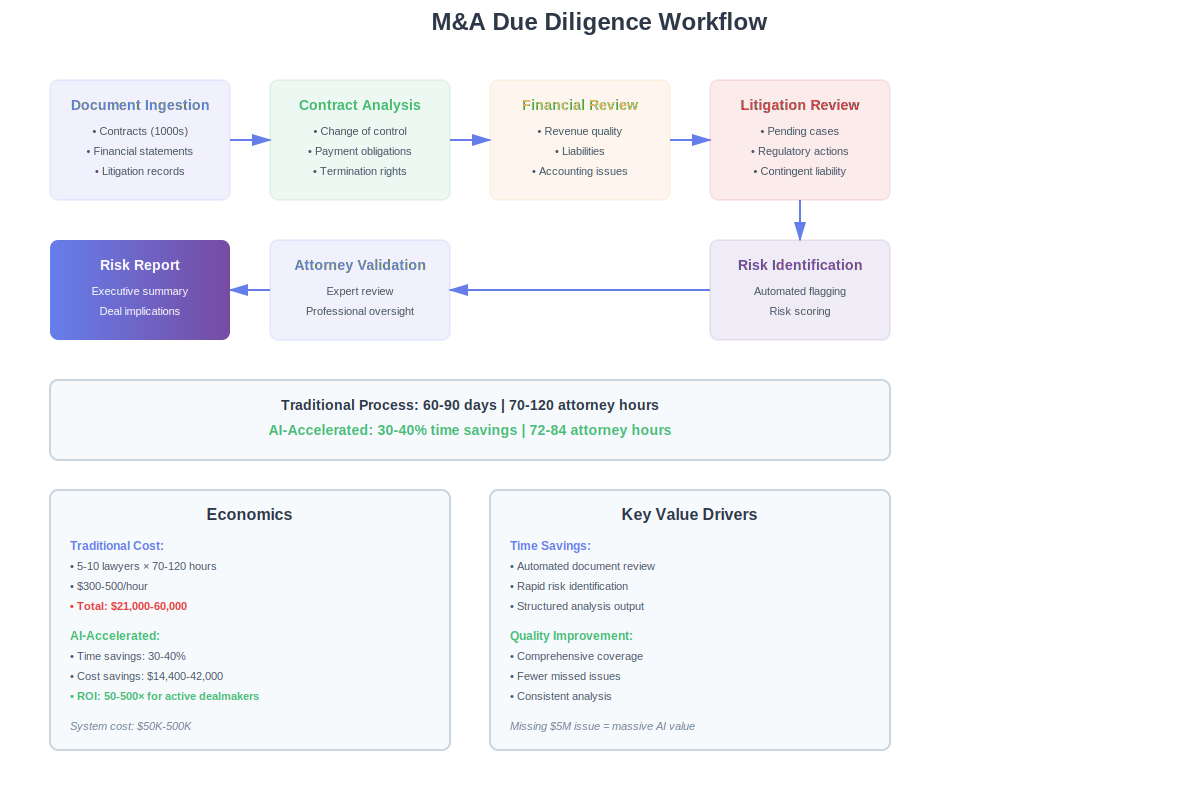
\includegraphics[width=0.95\textwidth]{chapters/diagrams/chapter13_due_diligence_q1r2s3t4.png}
\caption{AI-assisted M\&A due diligence workflow showing document ingestion, contract portfolio analysis, financial statement review, litigation and contingent liability identification, and risk reporting. The system accelerates due diligence by 30--40\%, reducing attorney hours from 120 to 72--84 hours per transaction, with ROI reaching 50--500× for active dealmakers.}
\label{fig:due_diligence_workflow}
\end{figure}

\subsection{Due Diligence Process and Requirements}

M\&A due diligence investigates target companies before acquisition, identifying risks that affect deal price and post-acquisition integration. The process is time-critical---most transactions require completion within 60--90 days---and document-intensive, requiring review of thousands of contracts, financial statements, litigation records, and regulatory filings.

Financial due diligence reviews target company financial statements, identifying risks: undisclosed liabilities, revenue quality issues, accounting irregularities. Regulatory compliance due diligence identifies exposure to regulatory violations, pending enforcement actions, or compliance gaps. Contract and obligation analysis identifies commitments that will transfer to acquirer, including unusual or onerous terms.

Litigation and contingent liability review identifies potential legal exposure: pending litigation, regulatory investigations, product liability risks, environmental liabilities. Missing one material liability can affect deal economics by millions of dollars.

Environmental and compliance due diligence assesses exposure to environmental liabilities, occupational safety issues, and industry-specific regulations. Costs of environmental remediation, regulatory cleanup, or compliance improvements can be substantial.

Intellectual property portfolio review identifies patent, trademark, and trade secret assets; assesses infringement risks; and evaluates freedom to operate in key markets.

\subsection{AI-Assisted Due Diligence}

AI systems accelerate due diligence by automating document review and risk identification. The process typically involves: document ingestion and classification, contract and financial analysis, risk identification and flagging, executive summary generation, and attorney validation.

Contract portfolio analysis identifies key terms: payment obligations, renewal dates, termination conditions, change of control provisions. Many acquisition agreements include change of control clauses triggering events at acquisition (early termination, consent requirements, renegotiation), creating significant risk if missed. Models scan contracts to identify these clauses and highlight implications.

Financial statement analysis identifies risks in financial data: unusual revenue recognition, significant write-downs, contingent liabilities. While AI cannot perform full financial audits, it can flag patterns for accountant attention.

Litigation and contingent liability review scans legal documents, litigation records, and regulatory filings to identify potential exposure. Models identify cases involving the target company, regulatory investigations, and settlement agreements.

\subsection{Economic Impact and Feasibility}

Due diligence traditionally requires weeks of attorney and specialist time. A typical mid-market acquisition involves 5--10 lawyers spending 40--60 hours on contract review, 10--20 hours on compliance analysis, 20--40 hours on litigation/contingent liability. Total effort: 70--120 lawyer-hours at \$300--500 per hour = \$21,000--60,000.

AI acceleration of due diligence has two value components: time savings and quality improvement. Time savings of 30--40\% reduce attorney hours from 120 to 72--84 hours, saving \$14,400--42,000 per transaction. Quality improvement (fewer missed issues) is harder to quantify but potentially more valuable. Missing a material issue that later costs \$5 million represents massive value from AI that prevents the miss.

Deployment cost for due diligence systems ranges from \$50,000 to \$500,000 depending on customization and scope. At that cost, systems become profitable after 5--10 transactions. For active dealmakers, ROI reaches 50--500\times annually.

\section{Financial Compliance and Anti-Money Laundering}

\begin{figure}[htbp]
\centering
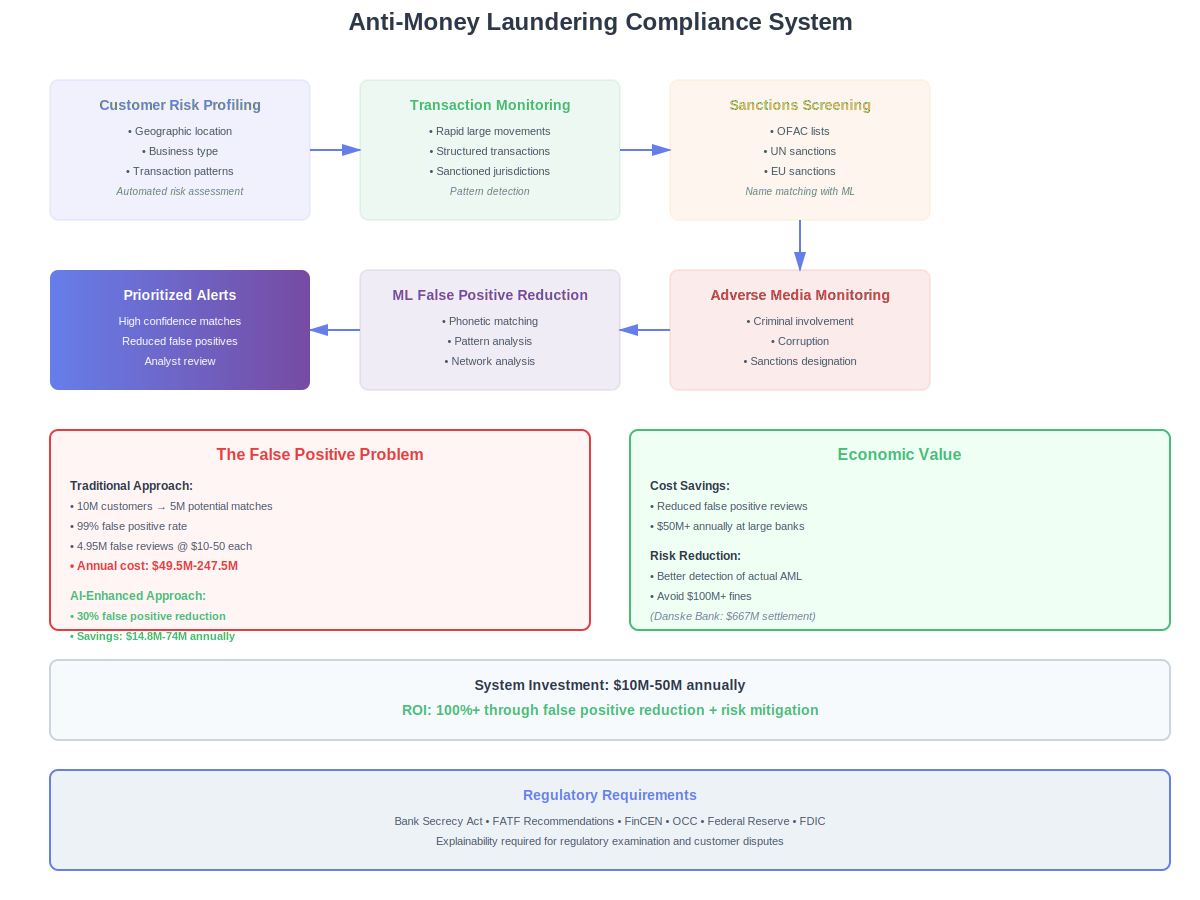
\includegraphics[width=0.95\textwidth]{chapters/diagrams/chapter13_aml_compliance_u5v6w7x8.png}
\caption{Anti-money laundering compliance system showing customer risk profiling, transaction monitoring, sanctions screening, and adverse media monitoring. The system reduces false positive alerts by 30\%, saving \$14.8--74 million annually at large institutions while improving detection of actual suspicious activity.}
\label{fig:aml_compliance_system}
\end{figure}

\subsection{Anti-Money Laundering and Sanctions Compliance}

Financial institutions are required by law (Bank Secrecy Act, FATF recommendations) to prevent use of their systems for money laundering and terrorism financing. This requires customer due diligence at account opening, ongoing transaction monitoring, and suspicious activity reporting.

Customer risk profiling at account opening assesses risk based on customer characteristics: geographic location, business type, transaction patterns. High-risk customers require enhanced due diligence. Models assess risk automatically, applying regulatory rules and learned patterns from historical data. A customer establishing accounts through shell companies in high-risk jurisdictions triggers heightened scrutiny.

Transaction monitoring detects suspicious patterns: rapid movement of large sums, round-dollar transactions, structured transactions designed to evade reporting thresholds, transfers to sanctioned jurisdictions. Models learn normal patterns for customer types and flag deviations. A customer normally moving \$10,000 weekly but suddenly moving \$500,000 in single transactions triggers investigation.

Sanctions screening verifies customers and counterparties against sanctions lists (OFAC, UN, EU, jurisdiction-specific lists). Automated screening compares customer names against sanctions lists, with manual review of matches to avoid false positives. Name matching is challenging due to variations: John Smith vs. John T. Smith vs. J. Smith.

Adverse media monitoring tracks public news and information about customers and counterparties for negative information: criminal involvement, corruption, sanctions designation, bankruptcy. Models ingest news and financial data, identifying relevant adverse information.

\subsection{False Positive Problem and AI Solutions}

A major pain point in financial compliance is false positive alerts. A customer named Mohammad Hussein matching ``Mohammad Hussein'' on a terrorism watch list generates an alert, even though it's a common name. Banks receive millions of potential matches, most of which are false positives requiring manual review.

Each manual review costs approximately \$10--50 depending on complexity. For a bank with 10 million customers generating 5 million potential matches annually with 99\% false positive rate: 4.95 million false reviews cost \$49.5--247.5 million annually. Reducing false positives by 30\% saves \$14.8--74 million annually.

Machine learning models learn patterns distinguishing false positives from true positives. Name matching can consider soundex/phonetic similarity, transaction pattern matching, and network analysis. A ``Mohammad Hussein'' with normal transaction patterns and no adverse information is likely false positive. A ``Mohammad Hussein'' with suspicious transaction patterns, offshore accounts, and adverse media coverage is higher risk.

\subsection{Regulatory Drivers and Economic Value}

Regulatory agencies (FinCEN, OCC, Federal Reserve, FDIC) impose strict requirements and substantial penalties for compliance failures. A bank with inadequate AML controls faces fines of \$100 million+. The Danske Bank Latvia case resulted in \$667 million settlement. Compliance failure creates catastrophic risk.

The economic value of AI in AML is twofold: cost savings from reducing false positives and risk reduction from better detection. Cost savings of \$50 million annually at large institutions justify \$10--50 million annual system investment. Risk reduction of even 1\% improvement in catching actual money laundering saves tens of millions in avoided fines and remediation.

\subsection{Implementation Challenges}

AML systems must integrate with core banking platforms, transaction systems, and customer data systems. Integration complexity is substantial due to diverse legacy systems and regulatory requirements for audit trails and documentation. A bank might have 20+ systems requiring integration.

Tuning and optimization is essential. Model thresholds for alerts must balance detection (catching bad activity) against false positive burden. A threshold that catches 99\% of suspicious activity might generate 5 million false alerts; a threshold generating 1 million false alerts might miss significant activity. Finding the right balance requires continuous tuning based on analyst feedback.

Explainability is required for regulatory examination and customer disputes. When an account is blocked on AML grounds, the institution must explain why. Models must provide reasoning: which sanctions list triggered the match, which transaction patterns were suspicious, which adverse information was found.

\section{Regulatory Compliance and Risk Monitoring}

\subsection{Regulatory Text Characteristics}

Regulatory documents present unique challenges for NLP. Regulations span multiple jurisdictions with different legal frameworks, evolve continuously through amendments and new rulings, and contain complex cross-references. A single regulation might reference dozens of other regulatory provisions, statutes, and guidance documents.

Regulatory language combines prescriptive requirements with interpretive guidance. Some provisions specify exact requirements: ``must maintain records for seven years.'' Others provide principles-based guidance: ``implement appropriate safeguards.'' Models must distinguish mandatory requirements from recommended practices, as compliance obligations differ fundamentally.

Applicability determination requires understanding which regulations apply to specific organizations. A financial services firm might be subject to SEC regulations, state banking laws, international standards like Basel III, and jurisdiction-specific requirements. Models must determine applicability based on organization characteristics, business activities, and geographic scope.

Change detection and impact analysis represent critical capabilities. When regulations change, organizations must identify affected policies, procedures, and controls. Models must detect regulatory changes, assess their significance, and map them to internal compliance frameworks.

\subsection{Specialized Compliance Domains}

Healthcare compliance includes HIPAA, anti-kickback statutes, Stark law prohibitions on self-referral, and fraud and abuse regulations. Each requires different monitoring and documentation.

Environmental compliance includes EPA Clean Air and Water Act regulations, state environmental requirements, emissions reporting. Organizations managing hazardous materials or operating in sensitive environments face complex requirements.

Labor law compliance includes wage and hour requirements, workplace safety (OSHA), anti-discrimination laws. Employment practices must comply with evolving regulatory requirements.

Export control and sanctions compliance includes OFAC sanctions, EAR controls, ITAR restrictions. Organizations exporting goods or services must navigate complex international regulations.

Tax compliance includes transfer pricing documentation, tax reporting requirements, FATCA and CRS requirements. Tax regulations are complex and jurisdiction-dependent.

Product safety and recall regulations vary by industry and product type. Consumer products must comply with CPSC requirements; medical devices with FDA; pharmaceuticals with FDA.

\subsection{Compliance Monitoring Systems}

Regulatory monitoring systems track regulatory changes and assess their impact. These systems ingest regulatory updates from multiple sources and analyze them for relevance and impact.

Architecture typically combines document ingestion, change detection, relevance classification, and impact assessment. Natural language understanding enables automated relevance determination. Models analyze regulatory text to identify applicable industries, activities, and jurisdictions.

Entity and obligation extraction identifies regulatory requirements. Models extract: what must be done, by whom, by when, with what documentation. This structured extraction enables comparison with existing policies and identification of compliance gaps.

Risk scoring assesses compliance risk based on regulatory requirements, organizational controls, and violation history. Models analyze the gap between regulatory requirements and implemented controls.

Explainability is critical. Compliance officers must understand why the system flagged a requirement, which regulations are affected, and what evidence supports the assessment.

\subsection{Continuous Monitoring and Reporting}

Deployed compliance systems must continuously monitor for violations. Models analyze operational data---transaction logs, access records, system configurations---for compliance violations or risk indicators.

Regulatory reporting automates the process of generating required reports. Models extract relevant data, format it according to regulatory specifications, and generate submission-ready documents.

Audit support provides evidence and documentation for regulatory examinations. Models maintain detailed logs of monitoring, decisions, and actions, enabling rapid production of audit evidence.

\section{Legal Research and E-Discovery}

\subsection{Case Law Analysis and Legal Research}

Legal research involves analyzing vast corpora of case law, statutes, and legal commentary to find relevant precedents. Traditional research requires manually searching and reviewing hundreds or thousands of documents. Transformer-based systems accelerate this through semantic search, relevance ranking, and automated summarization.

Semantic search enables finding relevant cases based on legal concepts rather than keyword matching. An attorney searching for ``duty of care in autonomous vehicle accidents'' should find relevant cases even if they use different terminology. Models trained on legal text learn to recognize semantic equivalence across different phrasings of legal concepts.

Citation analysis reveals precedential relationships. Models analyze citation networks to identify influential cases, track how legal doctrines evolve, and assess the strength of legal arguments. A case cited by hundreds of subsequent decisions carries more precedential weight than one rarely cited.

Multi-document synthesis combines information from multiple sources to answer legal questions. A model might synthesize holdings from dozens of cases to identify the prevailing rule in a jurisdiction. This synthesis requires understanding legal reasoning and identifying consistent patterns.

Automated summarization reduces time attorneys spend reading lengthy opinions. Models generate summaries highlighting the key holdings and reasoning. Extractive summarization selects important sentences; abstractive summarization generates new text capturing key points.

\subsection{E-Discovery and Document Review}

E-discovery involves reviewing massive document collections to identify responsive materials for litigation. Document volumes in complex litigation reach millions, making manual review prohibitively expensive. Technology-assisted review (TAR) using machine learning reduces review costs by 40--70\%.

Predictive coding trains models on attorney-reviewed documents. Attorneys review a seed set, labeling documents as relevant or not. Models learn from these labels and predict relevance for remaining documents. Continuous active learning improves model performance iteratively by selecting documents for attorney review that will most improve accuracy.

Statistical validation ensures the review process is reliable. Courts require demonstrating that TAR achieved target recall (finding responsive documents) and precision. Models must achieve 75--85\% recall with measurable precision. This requires statistical sampling and validation throughout the review process.

Privilege review identifies attorney-client privileged communications that must be withheld. This requires understanding privilege concepts, recognizing attorney-client relationships, and identifying legal advice. Errors waive privilege, exposing confidential communications. Typical approach: models flag potential privilege documents for attorney review rather than making final determinations.

Class action discovery involves millions of documents across thousands of parties. Class actions require managing complexity of multiple plaintiffs, defendants, and relevant parties. E-discovery in class actions is particularly expensive and demanding.

\subsection{Litigation Risk and Outcome Prediction}

Early litigation risk prediction assesses which disputes are likely to escalate to litigation. Models trained on dispute history predict likelihood of litigation based on dispute characteristics. Early identification enables settlement discussions before litigation becomes inevitable.

Case outcome prediction estimates likelihood of winning or losing based on facts and law. Models learn from historical case outcomes, identifying patterns that correlate with success. While not perfect, case outcome prediction improves settlement negotiations by enabling realistic assessment of case value.

Damages estimation enables negotiating appropriate settlements. Models estimate likely damages based on case facts, comparable cases, and judicial patterns. Better estimates of case value enable more rational settlement.

Settlement prediction identifies disputes likely to settle and optimal settlement ranges. This enables focusing litigation resources on cases unlikely to settle while pursuing settlement discussions where settlement is probable.

\section{Patent and Intellectual Property}

\subsection{Patent Classification and Prior Art Search}

Patent classification and analysis helps organizations manage patent portfolios and assess IP strategy. Models classify patents by technology domain, identify relevant patents in prior art searches, and assess patent portfolio strength.

Prior art search identifies existing patents that anticipate or render obvious patent applications. Traditional prior art search by specialists costs \$5,000--20,000. Automated search reduces cost and improves comprehensiveness. Models trained on patent corpora can identify relevant prior art more systematically than keyword-based search.

Technology landscape analysis identifies emerging technologies, competitive threats, and partnership opportunities. Models analyze patent portfolios to identify areas where competitors are investing and areas where organizations have competitive advantages.

\subsection{Infringement Analysis and Patent Prosecution}

Infringement prediction assesses the likelihood that a competitor's product infringes a patent. This enables strategic decisions about enforcement and litigation risk. Models learn infringement patterns from historical cases.

Patent prosecution support helps during patent application process. Models analyze rejected applications to identify reasons for rejection and suggest modifications. Experienced models can identify claims likely to survive examination.

Patent validity assessment estimates the likelihood that a patent will survive validity challenges. Patents facing validity challenges (accused of being obvious or anticipated) can be evaluated using models trained on validity challenges.

Freedom to operate analysis assesses whether an organization's products might infringe third-party patents. This is critical for new product launches and determines strategy for design-around or licensing.

\subsection{Economic Value and Implementation}

Patent applications cost \$10,000--50,000. High-quality prior art search (\$10,000) and prosecution support (\$5,000--15,000) are necessary investments. AI-assisted prior art search and prosecution support can reduce costs by 30--50\%, saving \$3,000--10,000 per application.

Patent valuation for licensing or portfolio management requires assessing strength, breadth, and value. Better patent analysis enables better licensing negotiations and more strategic portfolio decisions.

\section{Privacy and Data Protection Compliance}

\subsection{GDPR and International Privacy Compliance}

GDPR (General Data Protection Regulation) and similar privacy laws create extensive requirements for handling personal data. Organizations must understand which regulations apply, what data they hold, how they process it, and how they protect it.

Data inventory and mapping identifies all personal data collected, where it's stored, how it flows through systems, and who accesses it. This mapping is complex for large organizations with decades of systems. Models can automate inventory by analyzing system logs, data flows, and access records.

Privacy impact assessments evaluate risk of new data processing. Models can identify high-risk processing based on data sensitivity, scope, and security measures, flagging for detailed analysis.

Consent management tracks what consents users have given for various data processing. Models manage consent state and ensure compliance with consent requirements.

\subsection{Data Subject Rights and Automation}

GDPR requires responding to data subject requests: right to access, right to deletion, right to portability, right to restrict processing. These requests require finding personal data, verifying identity, extracting relevant data, and responding within 30 days.

Automating data subject request response reduces manual effort. Models identify relevant data, extract it in required formats, and generate responses. For organizations receiving hundreds of requests monthly, automation reduces manual effort by 80\%+, saving thousands of dollars and improving compliance.

Automated deletion of personal data when retention periods expire ensures GDPR compliance. Models track retention requirements and trigger deletion workflows.

\subsection{Compliance and Risk Assessment}

Monitoring compliance with privacy requirements involves analyzing systems, processes, and data handling. Models assess risk of violations and identify areas requiring remediation.

International privacy landscape (GDPR, CCPA, LGPD, PDPA, PIPL) creates complex requirements varying by jurisdiction. Models must track applicable regulations, requirements, and compliance obligations for different regions.

\section{Explainability and Audit Requirements}

\subsection{Citation and Provenance}

Legal AI systems must provide citations to source documents supporting their outputs. When a system identifies a contract risk or flags a compliance issue, it must cite the specific contract clause or regulatory provision. This citation requirement differs from general AI applications where outputs need not be traceable to specific training examples.

Implementation requires attention mechanisms that track which input tokens influenced output predictions. Models must maintain mappings between predictions and source text, enabling retrieval of supporting evidence. For contract review, this means identifying which sentences support a risk assessment. For compliance monitoring, this means citing specific regulatory provisions.

Provenance tracking extends beyond individual predictions to training data and model versions. Organizations must document which data trained the model, when it was trained, and what version produced specific outputs. This documentation supports audit requirements and enables investigating errors or unexpected behaviors.

Confidence scoring provides transparency about prediction reliability. Models should indicate uncertainty, enabling users to apply appropriate scrutiny. High-confidence predictions might proceed with minimal review; low-confidence predictions require careful attorney examination. Calibrated confidence scores---where 90\% confidence means 90\% accuracy---enable risk-based review strategies.

\subsection{Explainable AI Techniques}

Attention visualization shows which input tokens the model focused on when making predictions. For contract review, attention maps reveal which clauses influenced risk assessments. For compliance monitoring, they show which regulatory provisions triggered alerts. This visualization helps attorneys understand and validate model reasoning.

Feature importance analysis identifies which document characteristics most influenced predictions. For e-discovery, this might reveal that certain sender-recipient combinations, subject line patterns, or terminology strongly predict relevance. Understanding these features enables attorneys to assess whether the model learned appropriate patterns or spurious correlations.

Counterfactual explanations show how changing input would change predictions. ``If this indemnification clause included a cap, the risk score would decrease from 8 to 5.'' These explanations help attorneys understand model behavior and identify specific changes that would affect risk assessments.

Rule extraction from neural models attempts to distill learned patterns into interpretable rules. While transformer models are not inherently rule-based, techniques exist to approximate their behavior with decision rules. These rules provide transparency but may not capture the full model complexity, requiring validation against model predictions.

\subsection{Professional Responsibility and Oversight}

Attorney oversight remains essential in legal AI applications. Professional responsibility rules require attorneys to supervise AI systems and maintain ultimate responsibility for legal work product. This means attorneys must review and validate AI outputs, not merely accept them uncritically.

Competence requirements mandate that attorneys understand the AI systems they use. Attorneys must know the system's capabilities and limitations, understand when it's likely to make errors, and recognize situations requiring additional scrutiny. This requires training attorneys on AI fundamentals and system-specific characteristics.

Confidentiality obligations affect AI deployment decisions. Sending client documents to cloud-based AI services may violate confidentiality duties without appropriate safeguards. Many law firms require on-premises deployment or use of services with specific confidentiality protections and business associate agreements.

Bias and fairness considerations apply to legal AI systems. Models trained on historical legal data may perpetuate biases in legal outcomes. For example, models trained on historical sentencing data might reflect racial disparities. Organizations must assess potential biases and implement mitigation strategies, particularly for systems affecting individual rights or opportunities.

\section{Economic and Operational Considerations}

\subsection{Law Firm and Legal Department Integration}

Legal AI systems must integrate with existing legal technology infrastructure: document management systems, case management platforms, e-discovery tools, and contract lifecycle management systems. Integration complexity often exceeds model development complexity, consuming 60--80\% of deployment effort.

Document management integration requires handling diverse file formats, metadata standards, and access controls. Legal documents span Word, PDF, email, and specialized formats. Models must process these formats reliably while respecting access controls and privilege designations. Integration projects typically require 6--12 months of engineering effort.

Workflow integration determines adoption success. Systems that disrupt attorney workflows face resistance; systems that integrate seamlessly encourage usage. Effective integration embeds AI capabilities in existing tools rather than requiring attorneys to use separate applications. For example, contract review capabilities might appear directly in the document management system.

Change management and training are critical for adoption. Attorneys accustomed to traditional research and review methods may resist AI-assisted approaches. Successful deployments include comprehensive training, clear communication about system capabilities and limitations, and ongoing support. Pilot programs with enthusiastic early adopters typically achieve better adoption than organization-wide mandates.

\subsection{Cost-Benefit Analysis}

Contract review economics depend on attorney time savings and review volumes. For a law firm with 50 attorneys spending 30\% of time on contract review at \$300--500 per hour, annual contract review costs are \$9--15 million. A 40--60\% time savings represents \$3.6--9 million in value. At \$100,000--300,000 annual system cost, ROI is 12--90\times.

Due diligence economics: 5--10 lawyers on transaction at 70--120 hours each at \$300--500/hour = \$21,000--60,000. Systems costing \$50,000--500,000 break even on 5--25 transactions. For active dealmakers, ROI reaches 50--500\times annually.

E-discovery economics are driven by document volumes and review costs. Traditional document review costs \$1--3 per document. For litigation involving 1 million documents, review costs reach \$1--3 million. Predictive coding reducing review by 50--70\% saves \$500,000--2.1 million per matter. At \$200,000--500,000 annual system cost, ROI is 1--10\times depending on matter volume.

AML compliance economics: Reducing false positives by 30\% at major institutions saves \$14.8--74 million annually. System costs of \$10--50 million annually are easily justified.

Compliance monitoring economics depend on regulatory complexity and compliance team size. For a financial services firm with 20 compliance professionals at \$150,000 average cost, annual compliance costs are \$3 million. A 20--30\% efficiency improvement represents \$600,000--900,000 in value. At \$150,000--400,000 annual system cost, ROI is 1.5--6\times.

Infrastructure costs for legal AI vary by application and deployment model. Contract review systems serving 100 attorneys require 1--2 GPUs, costing \$20,000--40,000 in capital or \$500--1,000 monthly in cloud costs. E-discovery platforms processing millions of documents require 4--8 GPUs, costing \$80,000--160,000 in capital or \$2,000--4,000 monthly. Compliance monitoring systems require 2--4 GPUs, costing \$40,000--80,000 in capital or \$1,000--2,000 monthly.

\subsection{Risk Management and Liability}

Error consequences in legal applications can be severe. Missing a critical contract clause might expose an organization to unlimited liability. Failing to identify a compliance requirement might result in regulatory violations and fines. Incorrectly withholding privileged documents might waive privilege. These high-stakes consequences require robust quality assurance and risk management.

Quality assurance processes include statistical validation, ongoing monitoring, and regular audits. Initial validation establishes baseline accuracy on representative document sets. Ongoing monitoring tracks performance over time, detecting degradation or emerging error patterns. Regular audits by legal experts assess whether the system maintains acceptable accuracy and identify improvement opportunities.

Liability allocation between AI vendors, law firms, and clients remains evolving. When an AI system makes an error, who bears responsibility? Current practice treats AI as a tool, with attorneys retaining professional responsibility for work product. This framework requires attorney review and validation of AI outputs, limiting automation benefits but providing liability clarity.

Insurance and indemnification provisions in AI vendor contracts address error risks. Organizations should negotiate appropriate liability caps, error and omission coverage, and indemnification for AI-related errors. Vendors typically limit liability to contract value, which may be inadequate for high-stakes legal applications. Organizations may need additional insurance coverage for AI-related risks.

\section{Key Insights}

\textbf{Explainability Is Non-Negotiable}: Legal applications require citations to source documents and transparent reasoning. Models must provide specific references to contract clauses, regulatory provisions, or case law supporting their outputs. This explainability requirement affects architecture decisions and limits the use of black-box models.

\textbf{Attorney Oversight Remains Essential}: Professional responsibility rules require attorneys to supervise AI systems and maintain ultimate responsibility for legal work product. This means AI augments rather than replaces attorney judgment, with human review remaining necessary for quality assurance and liability management.

\textbf{Due Diligence and AML Represent Major High-Value Opportunities}: While contract review attracts attention, due diligence in M\&A and AML compliance in financial services represent larger economic opportunities. Due diligence acceleration and AML false positive reduction both have 50--500\times ROI potential.

\textbf{Domain Specialization Provides Significant Value}: Legal-specific language models trained on legal corpora achieve 5--8\% better performance than general models. This improvement translates to thousands of correctly identified clauses and obligations in production deployment, justifying the investment in domain-specific training.

\textbf{Integration Complexity Exceeds Model Complexity}: Legal AI systems must integrate with document management systems, case management platforms, and existing workflows. This integration typically consumes 60--80\% of deployment effort and determines adoption success more than model performance.

\textbf{Economic Value Varies Dramatically by Application}: Contract review provides 12--90\times ROI through attorney time savings. E-discovery provides 1--10\times ROI. Due diligence provides 50--500\times ROI for active dealmakers. AML compliance provides 100\%+ ROI through false positive reduction. Organizations should evaluate each application on its specific economics.

\textbf{Privacy Compliance (GDPR, CCPA) Is Increasingly Important}: Automating data subject request response and privacy compliance monitoring provides major operational value. Privacy regulations will only increase in scope and stringency.

\textbf{Risk Management Requires Robust Quality Assurance}: High-stakes consequences of errors require statistical validation, ongoing monitoring, and regular audits. Organizations must implement quality assurance processes that detect errors before they cause harm, balancing automation benefits against risk exposure.

The next chapter examines finance and time series applications, where transformer models address forecasting, risk assessment, and trading with unique temporal modeling and regulatory requirements.



% Chapter 14: Finance and Time Series (4 pages)
% \chapter{Finance and Time Series}

\section*{Why This Matters}

Financial services present unique challenges for transformer deployment that distinguish them from other AI applications. Non-stationary data distributions where patterns shift unpredictably. Regulatory requirements for explainability where every decision must be justified. Extreme latency constraints for high-frequency trading measured in microseconds. Severe consequences for prediction errors where mistakes cost millions. These constraints fundamentally shape architectural decisions, validation strategies, and deployment approaches.

The financial domain spans diverse applications with different technical requirements. Algorithmic trading requires sub-millisecond latency and robust handling of regime changes. Credit risk assessment demands explainability and fairness constraints. Anti-money laundering systems must balance detection accuracy against false positive burden while maintaining regulatory compliance. Fraud detection faces severe class imbalance with 99\% legitimate transactions. Each application requires specialized approaches that address its unique constraints.

Transformer architectures designed specifically for financial data address these challenges more effectively than standard models. Temporal Fusion Transformers handle multi-horizon forecasting with variable selection for time series. TabTransformers process categorical features more effectively than traditional gradient boosting for tabular data. Understanding when these specialized architectures justify their complexity—and when simpler approaches suffice—determines project success and cost efficiency.

This chapter examines three distinct financial applications: algorithmic trading with time series transformers, credit risk and fraud detection with tabular transformers, and anti-money laundering compliance systems. Each demonstrates different architectural choices, validation strategies, and deployment constraints that characterize production financial ML systems. The economic analysis reveals ROI ranging from 1--10× for e-discovery to 50--500× for AML compliance, with implementation costs from \$200,000 to \$50 million depending on scope and scale.

\section{Algorithmic Trading and Market Prediction}

Market prediction systems operate under constraints that distinguish them from other ML applications: non-stationary distributions where patterns shift unpredictably, microsecond latency requirements for high-frequency strategies, and direct financial consequences for every prediction error. These constraints shape every architectural and operational decision, from model selection through deployment infrastructure.

\subsection{Temporal Fusion Transformer Architecture}

The Temporal Fusion Transformer (TFT) addresses time series prediction through three specialized components: variable selection networks that identify relevant features from hundreds of candidates, temporal processing layers that capture patterns across multiple time scales, and multi-horizon prediction heads that forecast multiple time steps simultaneously. This architecture handles the complexity of financial time series more effectively than standard transformers designed for language.

\begin{figure}[htbp]
\centering
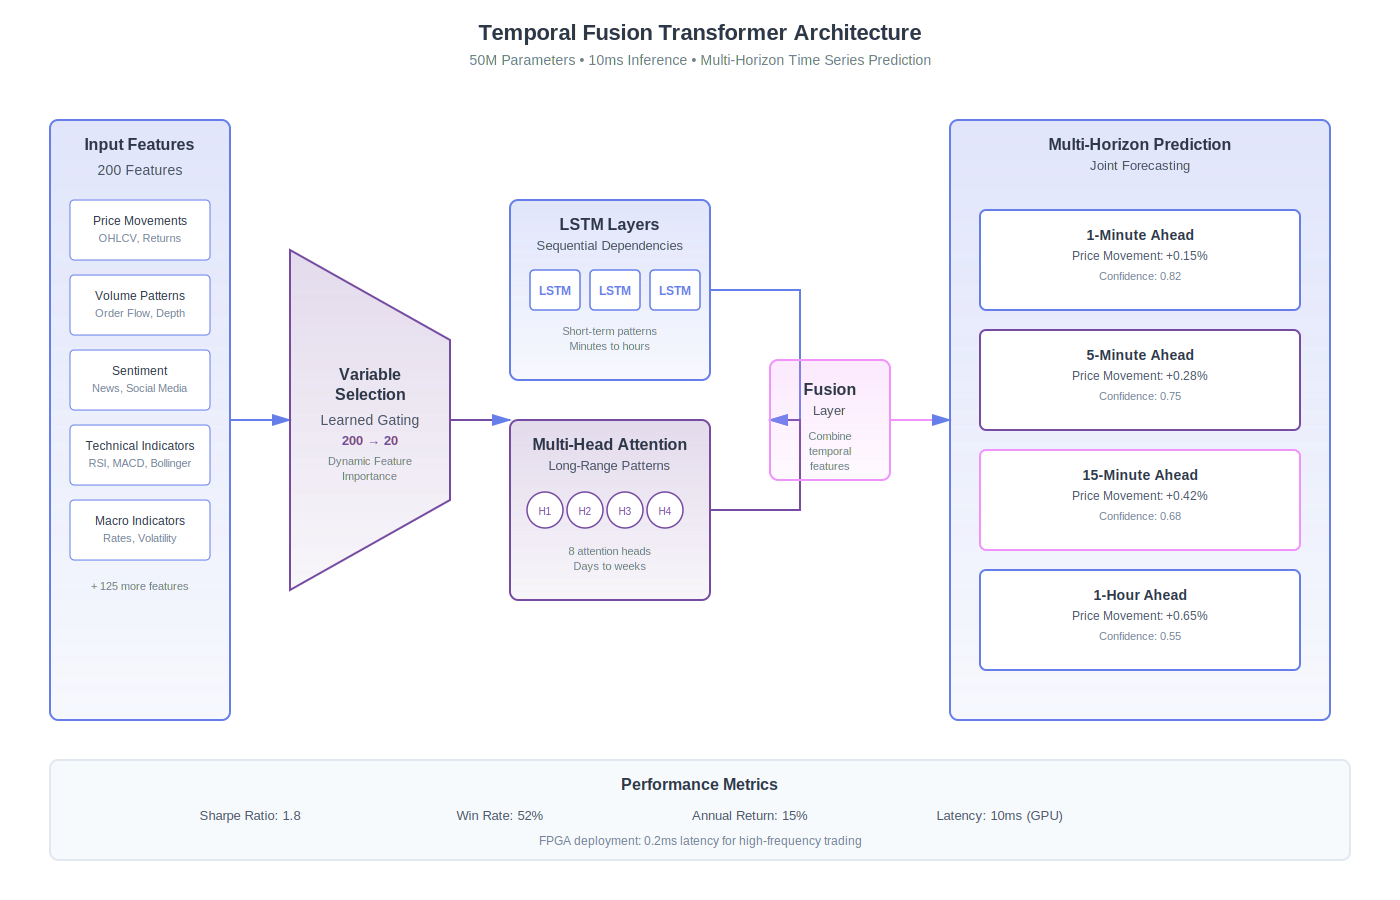
\includegraphics[width=0.95\textwidth]{chapters/diagrams/chapter14_tft_architecture_a1b2c3d4.pdf}
\caption{Temporal Fusion Transformer architecture showing variable selection network (200 to 20 features), LSTM layers for sequential dependencies, multi-head attention for long-range patterns, and multi-horizon prediction heads generating forecasts at 1-minute, 5-minute, 15-minute, and 1-hour horizons}
\label{fig:tft_architecture}
\end{figure}

Variable selection operates through learned gating mechanisms that weight input features dynamically. Given 200 potential features—price movements, volume patterns, order book depth, sentiment indicators, macroeconomic variables—the network learns to emphasize the 20 most predictive features for current market conditions. This selection adapts over time as market regimes change, unlike fixed feature engineering that requires manual updates.

The temporal processing architecture combines LSTM layers for sequential dependencies with multi-head attention for long-range patterns. LSTM components capture short-term momentum and mean reversion patterns spanning minutes to hours. Attention mechanisms identify longer-term relationships across days or weeks, such as earnings cycles or macroeconomic announcements. This hybrid approach handles both high-frequency patterns and structural market dynamics.

Multi-horizon prediction generates forecasts for multiple future time steps simultaneously—predicting price movements at 1 minute, 5 minutes, 15 minutes, and 1 hour ahead in a single forward pass. This joint prediction captures relationships between different time horizons more effectively than training separate models. A 50-million parameter TFT model processes 200 features and generates 4-horizon predictions in approximately 10 milliseconds on GPU hardware.

\subsection{Walk-Forward Validation and Lookahead Bias}

Financial time series validation requires walk-forward testing that simulates actual trading conditions. Standard k-fold cross-validation introduces lookahead bias—training on future data to predict the past—that produces misleadingly optimistic results. Walk-forward validation trains on historical data, tests on subsequent periods, then retrains including the test period before advancing to the next window.

A typical walk-forward schedule trains on 2 years of data, tests on 1 month, then advances the window by 1 month. This process repeats across the entire historical period, generating performance metrics that reflect realistic trading conditions. For a 5-year backtest with monthly retraining, this requires 60 separate training runs. At 4 GPU-hours per training run on A100 hardware, the validation process consumes 240 GPU-hours at approximately \$600 in compute costs.

The computational expense increases substantially when optimizing hyperparameters. Testing 10 hyperparameter configurations across the same 60-month walk-forward schedule requires 2,400 GPU-hours—roughly \$6,000 in compute costs. This expense explains why financial ML teams typically limit hyperparameter search to critical parameters like learning rate, attention heads, and regularization strength, while fixing architectural choices based on domain knowledge.

Lookahead bias detection requires careful data pipeline design. Features must use only information available at prediction time. A common error: calculating technical indicators using the entire day's data when predicting intraday movements. Proper implementation calculates indicators using only data through the prediction timestamp. Similarly, fundamental data like earnings reports must use announcement dates, not report dates, to avoid incorporating information unavailable to traders.

\subsection{Adversarial Training for Non-Stationarity}

Financial markets exhibit non-stationarity—statistical properties change over time as market regimes shift. A model trained on low-volatility periods performs poorly during market stress. Adversarial training improves robustness by exposing the model to artificially perturbed data that simulates regime changes.

The adversarial training process generates synthetic examples by applying small perturbations to input features that maximize prediction error. These adversarial examples represent market conditions the model finds challenging—typically regime boundaries where patterns shift. Training on both original and adversarial examples improves performance during actual regime changes, though at the cost of slightly reduced performance during stable periods.

Implementation adds 30-40\% to training time, as generating adversarial examples requires additional forward and backward passes. For the 240 GPU-hour walk-forward validation, adversarial training increases compute to approximately 330 GPU-hours—roughly \$825 in costs. This investment proves worthwhile for strategies deployed during volatile periods, where regime robustness determines profitability.

\subsection{FPGA Deployment for Low Latency}

High-frequency trading strategies require sub-millisecond latency from signal generation to order execution. GPU inference, while fast for batch processing, introduces 5-10 milliseconds of latency from data transfer and kernel launch overhead. FPGA deployment achieves 0.2 millisecond latency by implementing the model directly in hardware logic.

FPGA implementation requires converting the trained model to fixed-point arithmetic and synthesizing neural network operations as hardware circuits. This conversion process, performed by specialized tools like Xilinx Vitis AI, takes 2-3 weeks of engineering time and requires careful validation to ensure numerical accuracy matches the original floating-point model. Quantization to 8-bit or 16-bit fixed-point typically introduces less than 1\% accuracy degradation for financial models.

Hardware costs differ substantially from GPU deployment. A high-end FPGA card costs \$5,000-\$10,000 with negligible operating costs beyond power consumption. A comparable GPU costs \$10,000-\$15,000 with similar power requirements. The FPGA advantage lies in latency, not cost or throughput. For strategies where microseconds matter—market making, arbitrage, momentum trading—FPGA deployment justifies the engineering investment. For longer-horizon strategies, GPU inference suffices.

\subsection{Ensemble Methods and Confidence Intervals}

Financial prediction systems typically deploy ensembles of 5-10 models trained with different random seeds, architectures, or data samples. Ensemble predictions average individual model outputs, while prediction variance across ensemble members provides confidence intervals. These confidence intervals inform position sizing and risk management decisions.

A prediction with narrow confidence intervals—high agreement across ensemble members—justifies larger position sizes. Wide confidence intervals indicate model uncertainty, suggesting smaller positions or avoiding the trade entirely. This risk-aware approach improves risk-adjusted returns substantially. A strategy with 52\% win rate and 1.8 Sharpe ratio using confidence-based position sizing might achieve only 1.2 Sharpe ratio with fixed position sizes.

Ensemble deployment multiplies inference costs by the number of models. A 5-model ensemble requires 5× the compute resources of a single model. For FPGA deployment at 0.2 milliseconds per model, a 5-model ensemble completes in 1 millisecond—still acceptable for high-frequency strategies. For GPU deployment, ensemble inference takes 50 milliseconds, limiting applicability to lower-frequency strategies.

\subsection{Performance Metrics and Economics}

Trading strategy performance uses risk-adjusted metrics rather than raw returns. Sharpe ratio—excess return divided by return volatility—measures risk-adjusted performance. A Sharpe ratio of 1.8 indicates the strategy generates 1.8 units of excess return per unit of risk, considered strong performance for quantitative strategies. Win rate—percentage of profitable trades—provides additional context. A 52\% win rate with proper risk management generates consistent profits.

Annual returns depend on capital allocation and leverage. A strategy generating 15\% annual return on \$10 million capital produces \$1.5 million in profits. Infrastructure costs include compute resources, data feeds, and operational expenses. For the TFT-based strategy described:

\begin{itemize}
\item Training and validation: \$6,000 annually (monthly retraining with hyperparameter optimization)
\item FPGA hardware: \$50,000 initial investment, \$5,000 annual maintenance
\item Market data feeds: \$200,000 annually (real-time tick data, order book depth)
\item Operational costs: \$500,000 annually (infrastructure, monitoring, risk management)
\end{itemize}

Total annual costs approximate \$800,000. With \$1.5 million in profits, net return reaches \$700,000 or 7\% on capital—attractive for institutional investors when considering risk-adjusted characteristics.

\section{Credit Risk Assessment and Fraud Detection}

Credit risk and fraud detection systems process structured tabular data with hundreds of features, many categorical. Traditional gradient boosting methods like XGBoost excel at this task, but transformer-based approaches offer advantages for categorical feature handling and transfer learning from related tasks. Understanding when transformers justify their complexity requires analyzing the specific characteristics of the prediction problem.

\subsection{TabTransformer Architecture}

TabTransformer adapts transformer architecture for tabular data by treating categorical features as tokens and applying self-attention to learn feature interactions. Continuous features pass through standard feed-forward layers, while categorical features receive learned embeddings that capture semantic relationships. This approach handles high-cardinality categorical features—merchant IDs, product categories, geographic regions—more effectively than one-hot encoding or target encoding used by tree-based methods.

\begin{figure}[htbp]
\centering
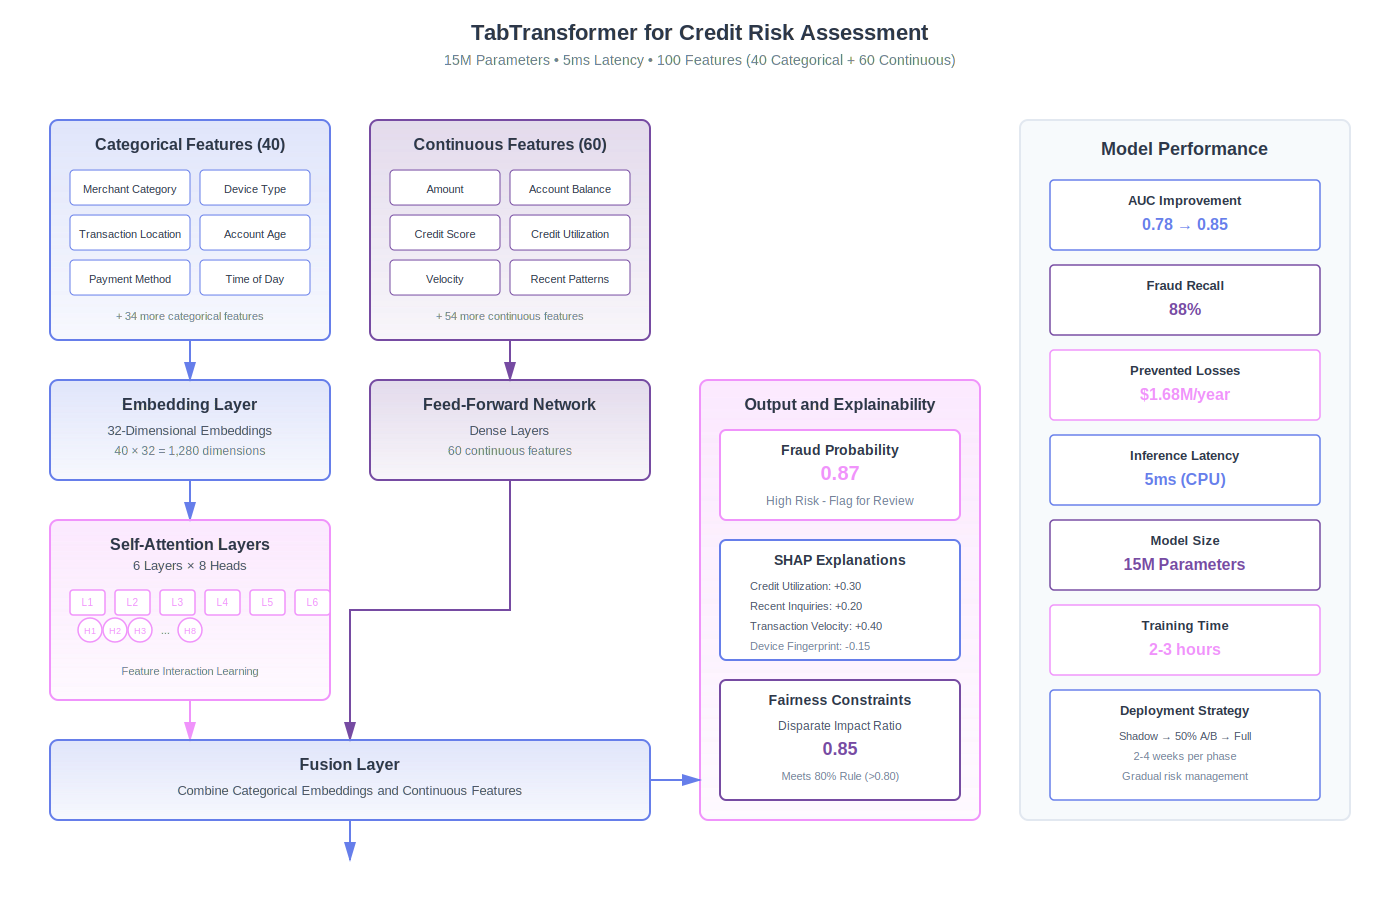
\includegraphics[width=0.95\textwidth]{chapters/diagrams/chapter14_credit_risk_model_e5f6g7h8.pdf}
\caption{TabTransformer architecture for credit risk assessment processing 40 categorical features through embedding and self-attention layers (6 layers, 8 heads) and 60 continuous features through feed-forward networks, with SHAP explainability and fairness constraint monitoring}
\label{fig:credit_risk_model}
\end{figure}

The architecture processes a credit application with 100 features: 40 categorical (merchant category, transaction location, device type, account age bucket) and 60 continuous (transaction amount, account balance, recent transaction patterns, credit utilization). Categorical features receive 32-dimensional embeddings, creating a 40×32 embedding matrix. Self-attention layers learn which categorical features interact—for example, that certain merchant categories combined with specific geographic regions indicate elevated fraud risk.

A typical TabTransformer for credit risk uses 6 attention layers with 8 heads each, totaling approximately 15 million parameters. This model size enables training on a single GPU in 2-3 hours using 1 million historical transactions. Inference latency reaches 5 milliseconds per prediction on CPU hardware, acceptable for real-time credit decisions that tolerate 100-200 millisecond total latency including data retrieval and business logic.

\subsection{Traditional and Alternative Data Features}

Credit risk models combine traditional credit bureau data with alternative data sources that provide additional signal. Traditional features include credit score, payment history, credit utilization, account age, and recent inquiries. Alternative data encompasses transaction patterns, device fingerprints, behavioral biometrics, social network indicators, and employment verification data.

Alternative data improves prediction accuracy for thin-file applicants—individuals with limited credit history—where traditional features provide insufficient signal. A model using only traditional features might achieve 0.78 AUC (area under ROC curve) on thin-file applicants, while adding alternative data improves AUC to 0.85. This 7-point improvement translates to substantial business value: approving more creditworthy applicants while maintaining fraud rates.

Feature engineering for alternative data requires domain expertise. Raw transaction data—timestamps, amounts, merchants—provides limited signal. Engineered features capture behavioral patterns: transaction velocity (transactions per day), amount distributions (mean, variance, percentiles), merchant diversity (unique merchants per month), and temporal patterns (weekday versus weekend spending). These engineered features often provide more signal than raw data.

\subsection{Class Imbalance and Focal Loss}

Fraud detection faces severe class imbalance: typically 1\% of transactions are fraudulent, 99\% legitimate. Standard cross-entropy loss trains models that predict "legitimate" for all transactions, achieving 99\% accuracy while catching zero fraud. Addressing class imbalance requires specialized loss functions and sampling strategies.

Focal loss down-weights easy examples—legitimate transactions the model predicts confidently—while emphasizing hard examples—fraudulent transactions the model finds challenging. The loss function includes a focusing parameter that controls this emphasis. For fraud detection with 1\% positive rate, focal loss with focusing parameter 2.0 typically improves fraud recall from 60\% to 88\% while maintaining precision above 80\%.

SMOTE (Synthetic Minority Over-sampling Technique) generates synthetic fraud examples by interpolating between existing fraud cases in feature space. This oversampling balances the training set, improving model sensitivity to fraud patterns. However, SMOTE can introduce artifacts if synthetic examples fall in regions of feature space that don't represent realistic fraud. Careful validation ensures synthetic examples improve rather than degrade model performance.

Combined approaches—focal loss during training with SMOTE oversampling—typically outperform either technique alone. Implementation requires careful hyperparameter tuning: SMOTE oversampling ratio (2:1, 3:1, or 5:1 fraud to legitimate), focal loss focusing parameter (1.5, 2.0, or 2.5), and class weights. Grid search across these parameters adds 20-30\% to training time but substantially improves fraud detection performance.

\subsection{Explainability and SHAP Values}

Financial services regulations require explainability for credit decisions—applicants must receive specific reasons for denial. SHAP (SHapley Additive exPlanations) values provide feature-level explanations by calculating each feature's contribution to individual predictions. For a denied application, SHAP values might indicate that high credit utilization contributed +0.3 to the fraud score, recent inquiries added +0.2, and unusual transaction velocity added +0.4.

Computing SHAP values requires multiple model evaluations per prediction—typically 100-500 evaluations to estimate feature contributions accurately. This computational cost makes SHAP impractical for real-time scoring of all transactions. Production systems compute SHAP values only for denied applications or flagged transactions requiring review, reducing the explanation workload to 1-2\% of total predictions.

SHAP values also enable model debugging and fairness analysis. Examining SHAP value distributions across demographic groups reveals whether the model relies on protected attributes or their proxies. If SHAP analysis shows that geographic features contribute disproportionately to denials for certain demographic groups, this indicates potential fairness issues requiring model adjustment or feature removal.

\subsection{Fairness Constraints and Disparate Impact}

Credit models must satisfy fairness constraints that limit disparate impact across demographic groups. Disparate impact measures the ratio of approval rates between groups—for example, approval rate for minority applicants divided by approval rate for majority applicants. Regulatory guidance typically requires this ratio to exceed 0.8 (the "80\% rule"), meaning minority approval rates must reach at least 80\% of majority approval rates.

Enforcing fairness constraints during training requires specialized optimization techniques. Post-processing approaches adjust decision thresholds separately for each group to achieve desired approval rate ratios. In-processing methods incorporate fairness constraints directly into the loss function, penalizing predictions that increase disparate impact. These techniques typically reduce overall model accuracy by 1-2 percentage points while ensuring fairness requirements.

Fairness-accuracy trade-offs require business judgment. A model achieving 0.87 AUC with 0.85 disparate impact ratio might be preferable to a model with 0.88 AUC and 0.75 disparate impact ratio, despite lower accuracy. The fairness improvement reduces regulatory risk and reputational harm, while the accuracy decrease has minimal business impact. Quantifying these trade-offs requires collaboration between ML teams, legal counsel, and business stakeholders.

\subsection{A/B Testing and Gradual Rollout}

Production deployment of credit models follows a gradual rollout strategy that manages risk while gathering performance data. The rollout typically progresses through three phases: shadow mode, partial deployment, and full deployment. Each phase validates model performance before expanding scope.

Shadow mode runs the new model alongside the existing production model, generating predictions without affecting decisions. This phase validates that the model performs as expected on production data, identifies data pipeline issues, and establishes baseline performance metrics. Shadow mode typically runs for 2-4 weeks, processing all production traffic while making zero business impact.

Partial deployment routes a percentage of traffic—typically 10-20\% initially, expanding to 50\%—to the new model while the existing model handles remaining traffic. This A/B test measures business impact: approval rates, fraud rates, revenue, and customer satisfaction. Statistical significance requires 2-4 weeks depending on traffic volume. For a system processing 100,000 applications daily, 2 weeks of 50\% traffic provides sufficient data to detect 0.5 percentage point differences in fraud rates with 95\% confidence.

Full deployment occurs only after partial deployment demonstrates improved or equivalent performance across all metrics. Even after full deployment, the previous model remains available for rapid rollback if issues emerge. This cautious approach prevents catastrophic failures that could result from deploying an untested model to all traffic immediately.

\subsection{Business Impact and Economics}

Credit risk model improvements translate directly to business value through increased approvals of creditworthy applicants and reduced fraud losses. A model improving AUC from 0.78 to 0.85 enables approving an additional 5\% of applicants while maintaining the same fraud rate, or maintaining the same approval rate while reducing fraud by 30\%.

For a lender processing 1 million applications annually with 60\% approval rate and 2\% fraud rate on approved applications, the business impact calculation proceeds as follows. The baseline system approves 600,000 applications with 12,000 fraud cases. At \$500 average loss per fraud case, annual fraud losses reach \$6 million. The improved model with 88\% fraud recall (up from 60\%) catches 10,560 fraud cases instead of 7,200, preventing an additional 3,360 fraud cases worth \$1.68 million annually.

Alternatively, maintaining the same fraud rate while increasing approvals generates revenue from additional customers. Approving 5\% more applicants—30,000 additional approvals—generates revenue from interest and fees. At \$200 annual revenue per customer, this produces \$6 million in additional annual revenue. The optimal strategy depends on business priorities: growth versus risk management.

Model development and operational costs include:

\begin{itemize}
\item Initial development: \$200,000 (3 months, 2 ML engineers, 1 data scientist)
\item Training infrastructure: \$10,000 annually (GPU compute for monthly retraining)
\item Inference infrastructure: \$50,000 annually (CPU servers for real-time scoring)
\item Monitoring and maintenance: \$100,000 annually (1 ML engineer part-time)
\item Data costs: \$500,000 annually (alternative data sources, credit bureau data)
\end{itemize}

Total annual costs approximate \$660,000 after initial development. With \$1.68 million in prevented fraud losses or \$6 million in additional revenue, the ROI justifies the investment substantially. The payback period for initial development costs reaches 2-3 months.

\section{Portfolio Optimization and Asset Allocation}

\subsection{Modern Portfolio Theory and Efficient Frontier}

Portfolio optimization determines optimal allocation of capital across multiple assets to balance return and risk. Traditional approaches use Markowitz mean-variance optimization, allocating weights to minimize portfolio volatility for a given expected return, or maximize return for a given volatility constraint.

The efficient frontier represents the set of optimal portfolios dominating all others—no other portfolio achieves higher return for the same risk or lower risk for the same return. Optimal portfolio allocation typically involves 10-50 different assets, with weights changing monthly as return expectations and correlations evolve.

Constrained optimization handles real-world constraints: sector exposure limits (maximum 30\% in technology), concentration limits (maximum 10\% per single stock), leverage limits, and dividend yield requirements. These constraints often have greater impact on performance than the optimization algorithm itself.

\subsection{Machine Learning Improvements Over Traditional Approaches}

Traditional mean-variance optimization struggles with three problems: correlation estimates are unstable and highly uncertain, expected returns are impossible to forecast accurately, and constraints are hard-coded and inflexible.

Machine learning approaches address these limitations through several mechanisms. Correlation prediction models learn which correlations are stable and which time-varying. During market stress, normally low-correlation assets become highly correlated—a phenomenon that traditional approaches fail to anticipate.

Return forecasting uses models that predict returns conditional on market regime, valuations, sentiment, and other factors. These dynamic return forecasts improve portfolio optimization compared to assuming constant expected returns.

Constraint adaptation allows models to learn which constraints bind under different market conditions. During high-volatility periods, leverage constraints should tighten; during stable periods, they can loosen.

Regime-aware optimization recognizes that different optimization approaches suit different market regimes. During normal markets, mean-variance optimization works well. During stress periods, risk-parity or equal-weight approaches perform better. Models can identify the current regime and select appropriate optimization strategies.

Expected improvement over traditional approaches ranges from 0.5-1.5\% annual return improvement. For a \$1 billion portfolio, this translates to \$5-15 million annually.

\subsection{Rebalancing and Transaction Costs}

Portfolio rebalancing—adjusting weights back to optimal allocations—occurs periodically. Monthly rebalancing keeps weights close to optimal but incurs transaction costs. Quarterly or annual rebalancing reduces transaction costs at the expense of drift from optimal allocations.

Transaction costs include bid-ask spreads, commissions, and market impact of large trades. For a \$1 billion portfolio rebalancing 30\% of holdings monthly, transaction costs approximate 0.05-0.10\% of portfolio value, or \$500,000-1,000,000 annually. This transaction cost must be justified by performance improvements.

Multi-period portfolio optimization considers transaction costs explicitly, finding allocations that balance expected return against trading costs. Models can identify when rebalancing is worthwhile—when return improvement exceeds transaction costs—and when to skip rebalancing.

\section{Customer Lifetime Value and Churn Prediction}

\subsection{Customer Lifetime Value Prediction}

Customer lifetime value (CLV)—total profit a customer will generate over their relationship with the company—drives customer acquisition and retention decisions. Acquisition costs justify spending up to 30-50\% of expected CLV to acquire a customer. Retention spending should increase with CLV.

Predicting CLV from customer characteristics, product usage, and account history enables several strategic capabilities. Acquisition targeting focuses acquisition spending on customer segments with high CLV—mobile customers might have 3× CLV of web-only customers. Retention prioritization allocates more resources to retaining high-CLV customers and less to low-CLV customers. Product recommendations align with customer preferences and profitability, recommending higher-margin products to customers most likely to purchase them. Lifecycle management enables stage-specific actions for different customer phases: new customers need onboarding, mature customers need expansion opportunities, at-risk customers need retention outreach.

CLV models typically use gradient boosted models or neural networks to predict expected profit from historical customer data. Features include customer demographics, account tenure, product holdings, transaction volumes, interaction history, and service quality metrics.

\subsection{Churn Prediction}

Churn prediction identifies customers likely to leave, enabling proactive retention outreach. For subscription businesses, even 5\% improvement in churn rates translates to 15-25\% revenue improvement through compounding over time.

Churn prediction models predict the probability that a customer will leave within a specified period—next month or next quarter. Customers with high churn risk receive targeted retention offers: service discounts, exclusive features, or personal support.

High-value customers warrant more aggressive retention spending. A model predicting 40\% churn risk for a \$10,000/month customer justifies offering \$2,000/month discounts—keeping the customer is worth \$8,000/month in retained revenue. For a \$100/month customer, the same intervention is not justified.

Churn models inform product development by identifying which feature gaps drive churn. If customers leaving use certain features less frequently, product improvements in those areas would reduce churn.

\subsection{Cross-Sell and Upsell Propensity}

Propensity models predict customer likelihood to purchase specific products. Product-specific models predict purchase probability for a particular product, such as an enterprise support add-on. General propensity models predict likelihood to buy any higher-value product.

Models identify which customer segments respond best to which offers. Email campaigns targeting customers most likely to purchase specific products achieve much higher response rates than mass marketing.

Timing models predict when customers are most receptive to offers. Recent product switchers might be more open to upgrade offers. Customers who just had negative support interactions might be more responsive to win-back offers.

\subsection{Economics and Implementation}

For a SaaS company with 100,000 customers averaging \$200 monthly (\$24 million annual revenue), the business impact breaks down as follows.

Churn improvement from reducing 5\% churn to 4\% through improved retention retains an additional \$2.4 million in revenue annually. At \$1,000 cost per retained customer, this generates \$1.4 million net value.

CLV improvement through more accurate prediction improves acquisition targeting and retention prioritization. Better targeting improves acquisition ROI by 10-20\%, translating to \$2-4 million annual value for acquisition budgets.

Implementation requires integrating CLV and churn models with customer success and marketing systems. Models score all customers weekly, generating lists of high-churn-risk, high-CLV customers for proactive outreach. Integration typically costs \$50,000-100,000; annual system costs approximate \$100,000.

With \$3-5 million annual value and \$100,000 annual costs, ROI reaches 30-50×.

\section{Feature Engineering and Data Quality}

\subsection{Data Quality and Missing Data}

Financial data quality varies dramatically. Real-time trading data is clean and complete. Alternative data sources like satellite imagery or credit card data have inconsistent coverage and gaps. Feature engineering and quality assurance consume 40-60\% of financial ML project effort.

Missing data requires careful handling. Simple approaches like mean imputation introduce bias. Domain-aware approaches—recognizing that missing volume data implies a liquidity event—preserve information better. Multiple imputation provides uncertainty estimates for downstream analysis.

Outliers require investigation rather than automatic removal. A 50\% stock price move is unusual but legitimate, reflecting an earnings surprise. A 5,000\% move is likely a data error. Domain expertise distinguishes legitimate outliers from errors.

\subsection{Feature Engineering from Raw Data}

Raw financial data—OHLCV (open, high, low, close, volume)—provides limited predictive signal. Feature engineering constructs more predictive variables.

Technical indicators like moving averages capture trend, RSI measures momentum, and Bollinger Bands indicate volatility. These indicators are computed from only historical data through the prediction timestamp, avoiding lookahead bias.

Market microstructure features including order book depth, bid-ask spreads, and order imbalance indicate market stress and short-term price direction.

Temporal features capture time of day, day of week, proximity to market opens and closes, and proximity to earnings dates, revealing seasonal and event-driven patterns.

Cross-sectional features measure relative performance—stock performance relative to sector—correlation changes, and price momentum relative to peers.

Proper feature engineering requires deep financial domain knowledge. Implementing features incorrectly, such as introducing lookahead bias in indicators, produces results that pass validation but fail in production.

\subsection{Feature Selection and Dimensionality}

Financial models often have 500+ features. Not all are predictive; many are noisy or redundant. Feature selection reduces noise and improves generalization.

Correlation analysis identifies redundant features. If two features are 0.95 correlated, they provide similar information and one can be removed. However, intentional correlation—different technical indicators measuring trend—can be valuable.

Importance-based selection ranks features by their contribution to predictions. Tree-based models provide built-in importance measures. Neural networks require SHAP or other explainability techniques. Selecting top-K features, such as the top 50 of 500, significantly reduces model complexity while often improving generalization.

Stability analysis measures whether feature importance changes over time. Features that are critical during some periods but irrelevant during others require regime-specific feature selection.

\section{Model Monitoring and Governance}

\subsection{Performance Monitoring and Degradation}

Deployed financial models degrade over time as market regimes change and data distributions shift. Regular monitoring detects degradation before it causes significant losses.

Performance metrics tracked continuously include prediction accuracy, Sharpe ratio, win rate, and fraud detection recall and precision. Alerts trigger when metrics fall below thresholds. For example, if fraud detection recall drops below 80\%, the system alerts for model investigation.

Performance decomposition identifies where degradation occurs. Degradation might be concentrated in certain market regimes like high-volatility periods, certain customer segments such as new account holders, or certain time periods like recent months. Targeted analysis identifies root causes.

\subsection{Data Drift and Concept Drift}

Data drift occurs when input distributions change, such as when an economic recession changes customer credit profiles. Concept drift occurs when relationships change, such as when a pandemic changes correlation between sectors.

Drift detection uses statistical tests to identify when distributions diverge significantly from training data. Sudden drift, like pandemic onset, requires immediate model retraining. Gradual drift, like slow economic deterioration, allows scheduled retraining.

\subsection{Retraining Frequency and Triggers}

Retraining frequency balances model freshness against computational cost. For algorithmic trading, daily or weekly retraining adapts to market changes. For credit models, monthly retraining suffices; annual retraining is insufficient.

Event-based retraining triggers when performance falls below thresholds, significant data drift is detected, major market events occur like crashes or policy changes, or regulatory changes require model adjustment.

Scheduled retraining ensures regular updates even if no specific event triggers retraining.

\subsection{Model Versioning and Governance}

Managing multiple model versions is essential for production systems. Key practices include version control to track all model code, training data, hyperparameters, and results, enabling reproduction of any model version.

Approval processes move models through stages—development, validation, production—with approval at each stage. Production models have clear ownership and governance.

Audit trails document when models were trained, on what data, with what performance, and when deployed, enabling investigation of model decisions.

Rollback capability maintains the ability to quickly revert to previous models if current models cause issues.

\section{When to Use Specialized Architectures}

\subsection{TabTransformer vs. XGBoost}

For credit risk prediction, does TabTransformer justify its complexity compared to XGBoost? A typical comparison reveals the trade-offs.

In terms of accuracy, TabTransformer achieves 0.85 AUC while XGBoost achieves 0.833 AUC. The 1.7 percentage point improvement represents reduced fraud. For a lender processing 1 million applications, this improvement prevents approximately 1,700 additional fraud cases at \$500 loss each, equaling \$850,000 annual value.

Development cost for TabTransformer requires 3 months with 2 engineers and 1 data scientist, totaling \$200,000. XGBoost requires 6 weeks at \$100,000. Additional development cost: \$100,000.

Operational cost for TabTransformer requires GPU infrastructure at \$10,000 annually. XGBoost requires CPU infrastructure at \$2,000 annually. Additional operational cost: \$8,000 annually.

ROI calculation: \$850,000 fraud prevention minus \$100,000 additional development minus \$8,000 annual operational cost equals \$742,000 annual net value. This ROI justifies TabTransformer investment.

However, if fraud improvement were only 0.5 percentage points (\$250,000 annual value), the \$100,000 development investment would not be justified. The decision depends on the actual accuracy improvement, which requires empirical validation.

\subsection{Temporal Fusion Transformer vs. ARIMA}

For stock price forecasting, does TFT justify its complexity compared to statistical approaches?

In terms of accuracy, TFT achieves 0.52 Sharpe ratio while ARIMA achieves 0.38 Sharpe ratio. The improvement represents higher risk-adjusted returns.

Development cost for TFT requires 4 months with 2 engineers, totaling \$150,000. ARIMA requires 2 weeks at \$10,000. Additional cost: \$140,000.

Operational cost for TFT requires GPU infrastructure at \$50,000 annually. ARIMA requires CPU at \$5,000. Additional cost: \$45,000.

Strategy value: For \$10 million capital, TFT Sharpe of 0.52 generates approximately \$1.2 million in annual returns. ARIMA generates approximately \$900,000. Additional value: \$300,000.

ROI calculation: \$300,000 annual returns minus \$140,000 development minus \$45,000 operational equals \$115,000 annual net value. This ROI justifies TFT investment.

However, this assumes the Sharpe ratio improvement actually occurs in production. Backtests often overestimate performance due to lookahead bias and overfitting. If production performance shows only 0.05 Sharpe improvement instead of 0.14, the value drops to \$50,000 annually, which barely justifies investment.

\subsection{The Importance of Empirical Validation}

The decision to deploy specialized architectures must be based on empirical validation, not theoretical arguments. A model that achieves 0.01 percentage point improvement in backtests but fails in production provides no value despite theoretical justification.

Key validation principles include walk-forward validation that simulates production conditions, out-of-sample validation on completely held-out data, pilot deployment before full rollout, and realistic performance estimation accounting for overfitting risk.

\section{Regulatory Framework and Compliance}

\subsection{Model Risk Management}

Federal Reserve guidance (SR 11-7) establishes Model Risk Management requirements for large financial institutions. Key requirements include model validation through independent validation before and after deployment, including performance monitoring and stress testing.

Model governance requires clear policies, procedures, and oversight. Models must be approved before deployment and re-approved periodically.

Risk management assesses and manages risks from model errors. Institutions must establish thresholds triggering model review or replacement.

\subsection{Stress Testing and CCAR/DFAST}

Comprehensive Capital Analysis and Review (CCAR) and Dodd-Frank Act Stress Testing (DFAST) require large banks to demonstrate capital adequacy under adverse scenarios. Models predict losses under various economic scenarios including recession, market crash, and unemployment spike.

These stress testing models often use machine learning to map economic scenarios to specific outcomes. Credit loss models, trading loss models, and operational risk models all require scenario analysis.

\subsection{Fair Lending Compliance}

The Equal Credit Opportunity Act requires that credit models not discriminate based on protected characteristics. Fair Lending exams scrutinize credit models for disparate impact. Models must demonstrate that differences in outcomes reflect legitimate creditworthiness factors, not protected characteristics or proxies.

\subsection{Market Abuse and Algorithmic Trading}

The Securities and Exchange Commission (SEC) and regulatory bodies scrutinize algorithmic trading for market manipulation. Models must be able to explain trading decisions and demonstrate that they do not engage in prohibited practices like spoofing, layering, or pump-and-dump schemes.

\section{Key Insights}

\textbf{Specialized Architectures Address Specific Data Characteristics}: Temporal Fusion Transformers for time series with variable selection and multi-horizon prediction. TabTransformers for tabular data with categorical features. Understanding whether data characteristics justify architectural complexity determines project success.

\textbf{Walk-Forward Validation Is Essential for Financial Applications}: Standard cross-validation introduces lookahead bias producing misleadingly optimistic results. Walk-forward testing correctly simulates production conditions but requires substantial compute. The \$600-6,000 validation cost for backtests is necessary investment, not optional optimization.

\textbf{Non-Stationarity Requires Adaptive Approaches}: Fixed models degrade as market regimes change. Adversarial training improves robustness. Frequent retraining adapts to changing conditions. Ensemble methods provide confidence intervals informing risk management.

\textbf{Latency Requirements Drive Deployment Architecture}: Sub-millisecond requirements drive FPGA deployment despite 2-3 weeks engineering effort. Millisecond-scale requirements use GPUs. Second-scale requirements use CPU. Understanding latency requirements before architecture selection prevents costly redesign.

\textbf{Class Imbalance Requires Specialized Techniques}: Fraud detection with 1\% positive rate requires focal loss and SMOTE. Standard cross-entropy loss produces models predicting "legitimate" for all transactions, achieving accuracy while catching zero fraud.

\textbf{Regulatory Requirements Are Non-Negotiable}: Fair lending compliance, model risk management, and stress testing requirements cannot be postponed. Compliance architecture decisions affect model design and deployment.

\textbf{Economic Justification Must Be Based on Empirical Validation}: Decisions to deploy specialized architectures must rest on production performance, not backtests. Overfitting in backtests produces overoptimistic estimates. Pilot deployment before full rollout validates assumptions.


% Chapter 15: Autonomous Systems and Observability (4 pages)
% \include{chapters/chapter15_autonomous_systems}

% Chapter 16: Synthesis and Future Outlook (1 page)
% \include{chapters/chapter16_synthesis}

% ============================================================================
% BACK MATTER
% ============================================================================
\backmatter

% Appendices
\appendix

% Appendix A: Mental Models and Decision Frameworks
% \include{chapters/appendix_mental_models}

% Appendix B: Cost Calculators and Worksheets
% \include{chapters/appendix_calculators}

% Appendix C: Vendor Evaluation Checklists
% \include{chapters/appendix_vendors}

% Appendix D: Further Reading and Resources
% \include{chapters/appendix_reading}

% Bibliography
\printbibliography[heading=bibintoc]

% Index
\printindex

\end{document}
